\documentclass[a4paper,12pt]{article}
\usepackage[utf8]{inputenc}
\usepackage[ngerman,german]{babel}
\usepackage[T1]{fontenc}
\usepackage{courier}
\usepackage{float}
\usepackage{amsmath,amsthm}
\usepackage{amssymb}
\usepackage{mathtools}
\usepackage{tabularx}
\usepackage{graphicx}
\usepackage{cite}
\usepackage{csquotes}
\usepackage {pdfpages}
\usepackage[font=small,labelfont=bf]{caption}
\usepackage[pages=some]{background} % Draft Wasserzeichen mit Option pages=all sonst pages=some

\newtheorem{Lemma}{Lemma}[section]
\newtheorem{Satz}{Satz}[section]


\begin {document}
\begin{center}

\includegraphics[width= 0.4\textwidth]{Medien/kleinkram/UniLogo}
\end{center}
\bigskip


 \begin{center}
 	\LARGE{Bachelorarbeit zum Thema\\
 	Tango Bäume}\\
 \bigskip
 \bigskip
 \bigskip
 \bigskip
\bigskip
\bigskip 
\bigskip
\bigskip
 \large{
 Andreas Windorfer\\
 q8633657}
 \end{center}
 \bigskip
 \bigskip
 \bigskip
 \bigskip 
 \bigskip
 \bigskip
 \bigskip 
  \bigskip 
 \bigskip
 \bigskip
 \bigskip 
  \begin{center}
 ausgeführt am\\
 Lehrgebiet Theoretische Informatik\\
 Leitung Prof. Dr. André Schulz\\
\end{center}

\author{Andreas Windorfer}





\newpage
\begin{center}
\textbf{Zusammenfassung}
\end{center}
 Bei binären Suchbäumen sind besonders die Ausführungszeiten ihrer Operationen von Interesse. Hier werden speziell die Ausführungszeiten von Folgen von \textit{access} Operationen betrachtet, im Bezug zur Anzahl der Knoten des binären Suchbaumes $n$. Beim 1985  vorgestellten Splay Baum \cite{splay} wird vermutet, dass dieser jede Folge von  \textit{access} Operationen asymptotisch betrachtet, mindestens genau so schnell ausführt, wie jeder andere binäre Suchbaum. Dies wurde als \enquote{Dynamische Optimalitäts Vermutung} bekannt. Bis heute ist offen, ob der Splay Baum diese Eigenschaft besitzt.  2007 wurde dann der Tango Baum  \cite{demainDinamicOpti} vorgestellt. Bei ihm ist bekannt, dass er jede solche Folge asymptotisch betrachtet, höchstens um einen Faktor $\log\left(\log\left(n\right)\right)$ langsamer ausführt, als der jeweils schnellste binäre Suchbaum. Um dies zu beweisen wurde die \enquote{Interleave Lower Bound}, eine untere Schranke für die Ausführungszeit solcher Folgen verwendet.  Bis dahin war für keinen binären Suchbaum ein Faktor kleiner als $\log\left(n\right)$ bewiesen und dieser wird von den balancierten binären Suchbäumen trivial erreicht. Der Tango Baum wird im Detail vorgestellt und zusätzlich noch zwei Variationen zu ihm. Abschließend werden Laufzeittests zwischen dem Tango Baum und dem Splay Baum durchgeführt, wobei der Splay Baum durchgängig die niedrigeren Zeiten liefern wird. 
\newpage
\tableofcontents
\newpage



\newpage
\section{Einleitung}
Binäre Suchbäume werden zur Lösung des Wörterbuchproblems eingesetzt. Hierbei existiert eine Menge von Schlüsseln, denen Daten zugeordnet sind. Im Telefonbuch wäre ein Name beispielsweise ein Schlüssel, dem als Datum eine Telefonnummer zugeordnet ist. Da solche Mengen von Schlüsseln in der Praxis extrem groß werden können, ist es wichtig, diese möglichst effizient zu verwalten. Auf einen einmal eingefügten Schlüssel kann beliebig oft zugegriffen werden. Deshalb müssen vor allem diese Zugriffe effizient sein. Das binäre Suchen bietet sich hierzu als Möglichkeit an. Die Schlüssel müssen dazu auf irgendeine Art und Weise sortiert vorliegen.\\ Beim Telefonbuch wird die alphabetische Sortierung verwendet. Somit kann mit der Suche eines Namens in etwa der Mitte des Telefonbuches gestartet werden. Nach einem Vergleich können dann zumindest die Schlüssel einer Hälfte des Buches ausgeschlossen werden. Dieses Verhalten iteriert bis der gesuchte Name gefunden ist. Obwohl es viele Varianten von binären Suchbäumen mit zum Teil aufwändigem Verhalten gibt, ahmen sie im Grunde das binäre Suchen nach.\\
Binäres Suchen könnte jedoch auch mit einem einfachen Array umgesetzt werden. Hierbei ergibt sich bei Änderungen an der Schlüsselmenge jedoch das Problem, das Array effizient anzupassen. Wird z.B. ein Schlüssel entfernt, müssen alle Nachfolgenden um ein Feld verschoben werden. Beim Einfügen eines Schlüssels könnte sogar ein Umzug in ein größeres Array notwendig werden. Bei binären Suchbäumen können solche Änderungen effizienter durchgeführt werden.\\ 
Das Auffinden eines Schlüssels erfolgt beim binären Suchbaum  mit einer \mbox{\textit{access}} Operation.  Eine Eigenschaft des binären Suchbaumes ist es, dass weiter oben liegende Schlüssel schneller erreicht werden können als andere. Ist bekannt, wie häufig auf welchen Schlüssel zugegriffen wird, kann diese Eigenschaft ausgenutzt werden. Ein Schlüssel wird dann umso weiter oben platziert, je häufiger auf ihn zugegriffen wird. \\
Ein weiterer Versuch ein  effizientes Verhalten zu erreichen sind die dynamischen binären Suchbäume. Im Gegensatz zu statischen binären Suchbäumen ändern diese ihre Struktur auch bei \textit{access} Operationen. Dies macht sie unabhängiger von den oft unbekannten Häufigkeiten der Zugriffe auf die einzelnen Schlüssel. Der Tango Baum ist ein solcher Vertreter, ebenso wie der Splay Baum, der in dieser Arbeit als Vergleichspartner dient.



\newpage
\section {Binäre Suchbäume}
Es gibt viele Varianten von binären Suchbäumen mit unterschiedlichen Eigenschaften und Leistungsdaten. In diesem Kapitel werden binäre Suchbäume im Allgemeinem beschrieben. Außerdem werden Begriffe definiert, die in den nachfolgenden Kapiteln verwendet werden. \\
\subsection {Die Definition des  binären Suchbaumes.}
Ein \textbf{Baum} $T$ ist ein minimal zusammenhängender gerichteter Graph. Ein Baum ohne Knoten ist ein \textbf{leerer Baum}. In einem nicht leeren Baum gibt es genau einen Knoten ohne eingehende Kante. Dieser wird als \textbf{Wurzel}  bezeichnet. Alle anderen Knoten haben genau eine eingehende Kante.  Enthält der Baum eine Kante von Knoten $v_1$ zu Knoten $v_2$, so ist $v_2$ ein \textbf{Kind} von $v_1$ und $v_1$ ist der  \textbf{Elternknoten} von $v_2$. Die Wurzel hat also keinen Elternknoten, alle anderen Knoten haben genau einen.  Ein \textbf{Pfad} $P$ ist eine Folge von Knoten $(v_0$,$v_1$,...,$v_n)$ mit $\forall i \in \{ 1, 2,..., n \} \colon v_{i-1}$ \textit{ist der Elternknoten von} $v_i$. $n$ ist die \textbf{Länge des Pfades}. $\left(v_0\right)$ ist ein Pfad der Länge $0$. Jeder Knoten $v$ in $T$ ist die Wurzel eines \textbf{Teilbaumes} $T(v)$. Dieser entsteht indem alle Knoten $u$ aus $T$ entfernt werden, zu denen es keinen Pfad mit  $v_0 = v$ und $v_n = u$ gibt. Knoten ohne ausgehende Kante werden \textbf{Blatt} genannt. Jeder andere Knoten wird als \textbf{innerer Knoten} bezeichnet.\\
Bei einem \textbf{binären Baum} kommt folgende Einschränkung hinzu:  \\
\textit{Ein Knoten hat maximal zwei Kinder.}\\ 
Entsprechend ihrer Zeichnung werden die Kinder in Binärbäumen als \textbf{linkes Kind} oder \textbf{rechtes Kind} bezeichnet. Sei $w$ das linke, bzw. rechte Kind von $v$, dann wird der Teilbaum mit der Wurzel $w$ als \textbf{linker Teilbaum}, bzw. \textbf{rechter Teilbaum}  von $v$ bezeichnet.  

\begin{figure}[H]
	\centering
	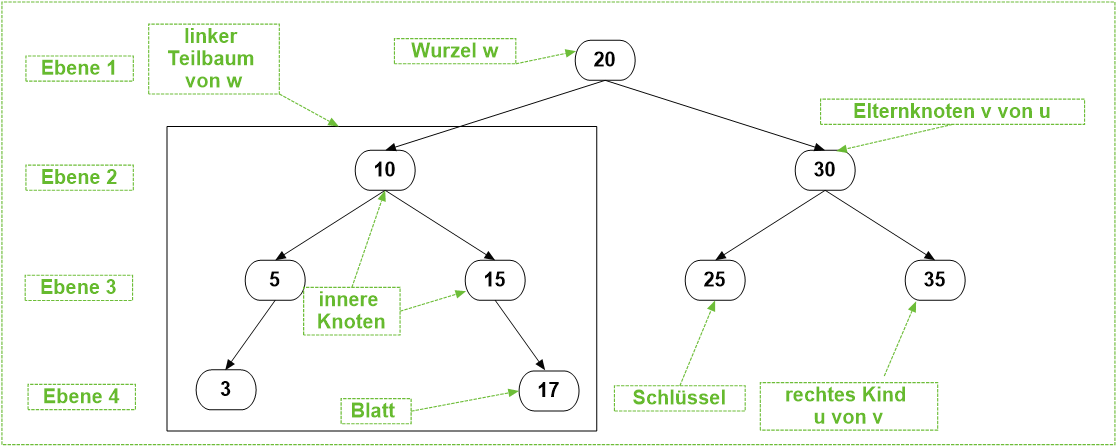
\includegraphics[width= 1\textwidth]{Medien/Einleitung/ioSuchbaum}
	\caption{Ein binärer Suchbaum. }
	\label{fig:ioSuchbaum}
\end{figure}
\begin{figure}[H]
	\centering
	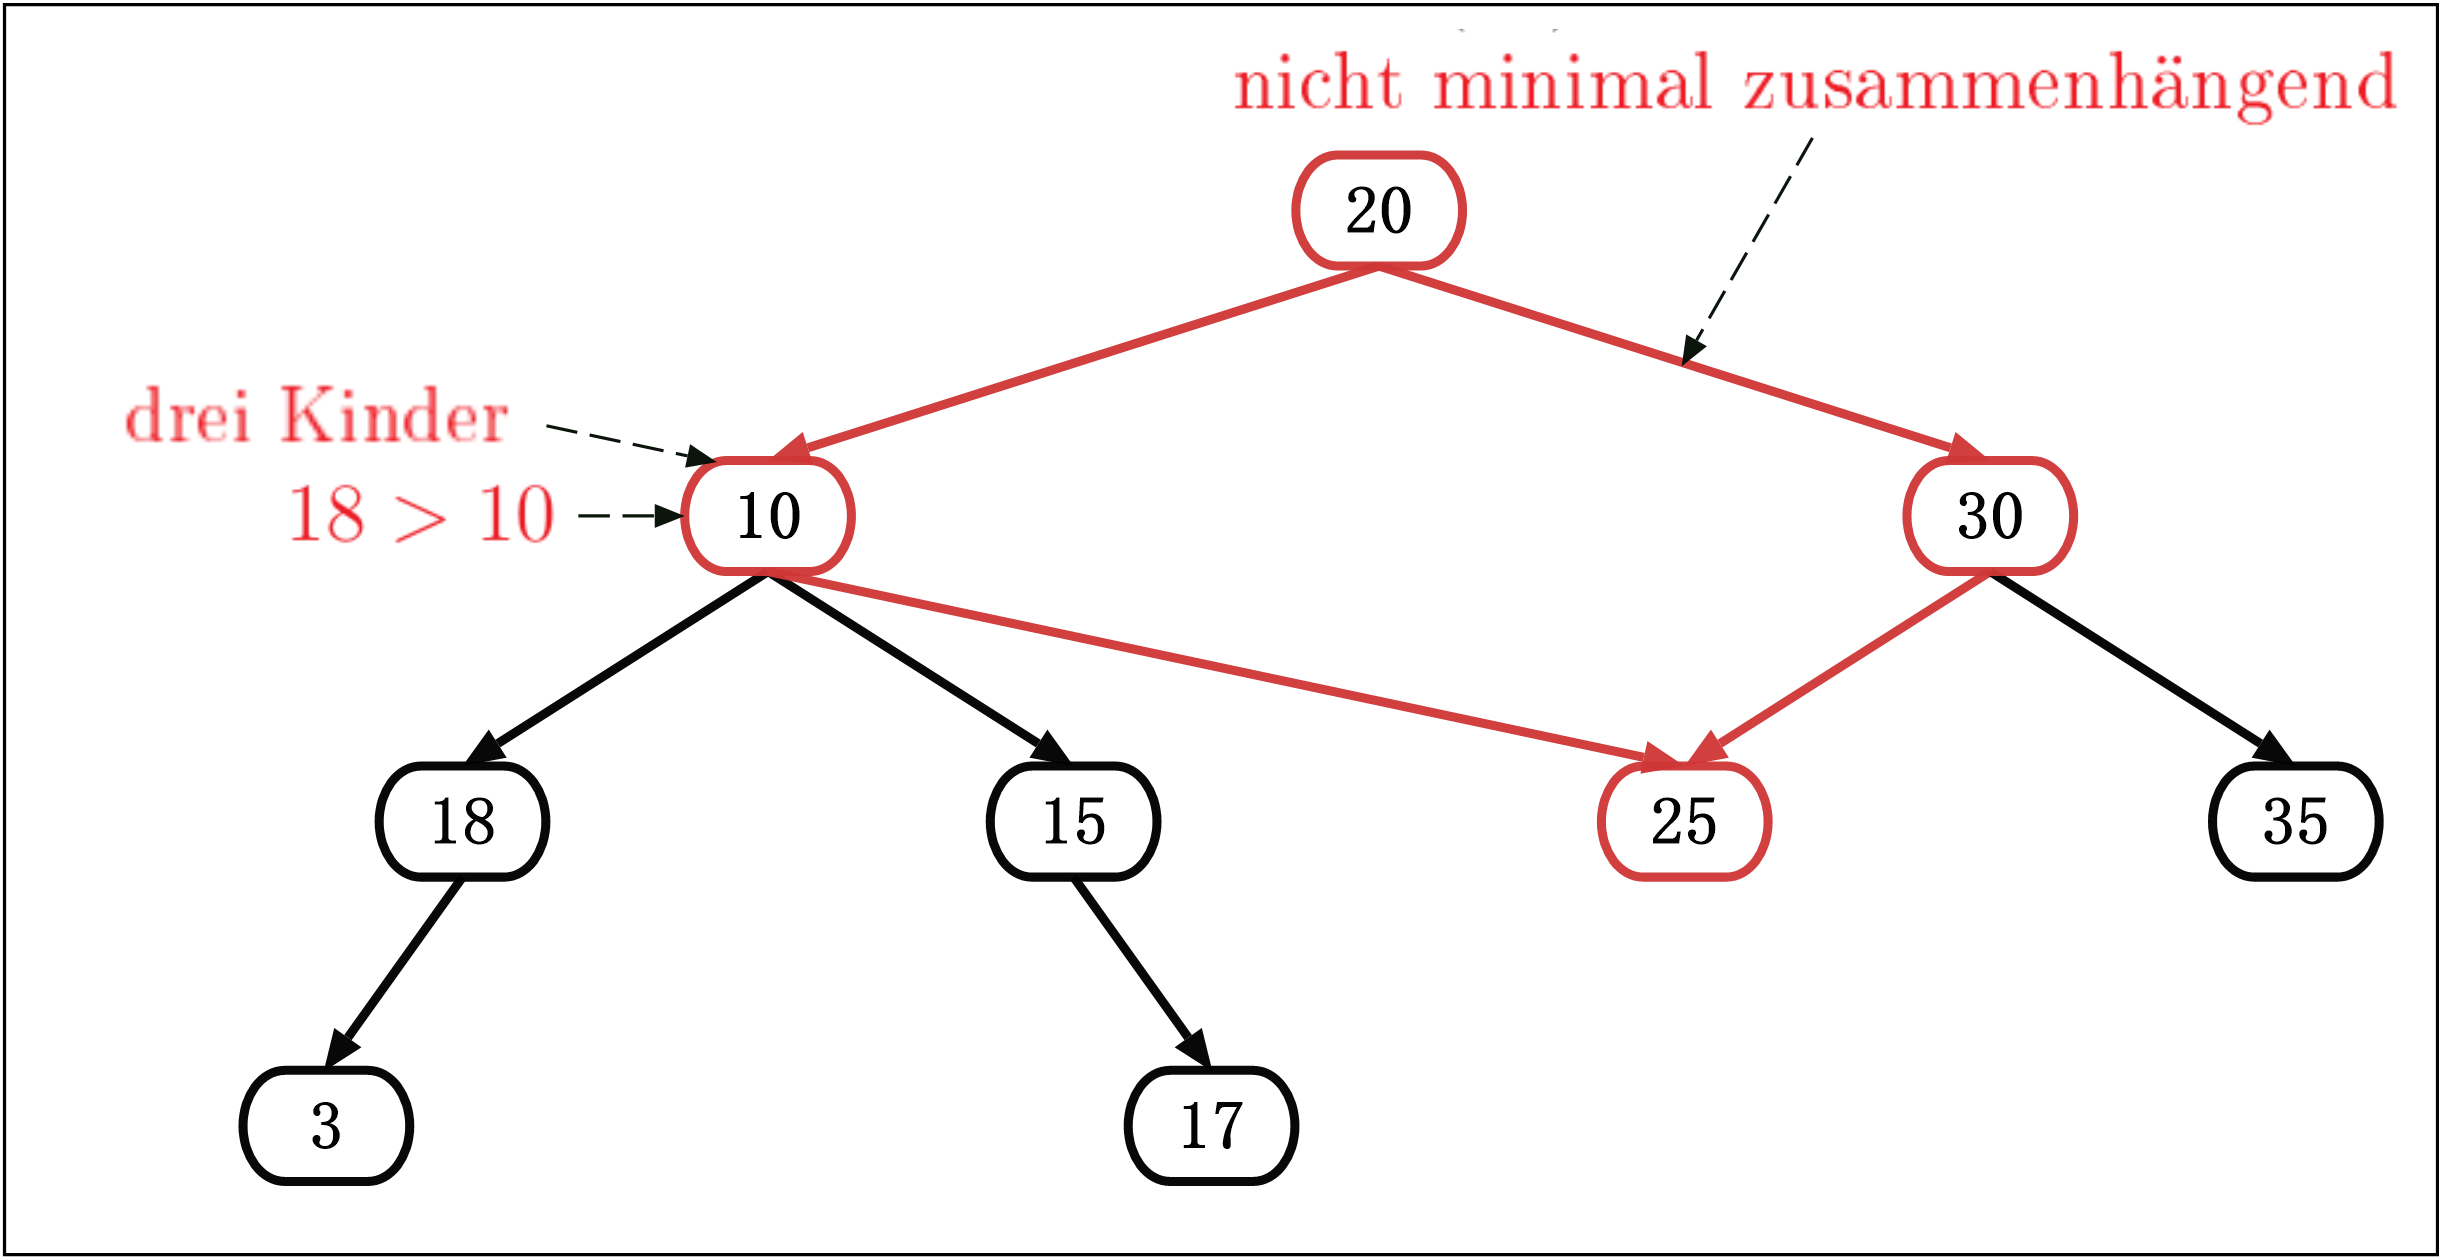
\includegraphics[width= 1\textwidth]{Medien/Einleitung/nioSuchbaum}
	\caption{Kein binärer Suchbaum. }
	\label{fig:nioSuchbaum}
\end{figure}

\noindent Bei einem \textbf{binären Suchbaum} ist jedem Knoten $v$ ein innerhalb der Baumstruktur eindeutiger \textbf{Schlüssel} $\mathit{key}\left(v\right)$ aus einem \textbf{Universum} zugeordnet, auf dem eine totale Ordnung definiert ist. Auf totale Ordnungen wird in diesem Kapitel noch eingegangen. Falls nicht explizit anders angegeben, wird hier und in den folgenden Kapiteln als Universum immer $\mathbb{N}$ verwendet, wobei die $0$ enthalten ist. Die in einem binären Suchbaum enthaltenen Schlüssel bezeichnen wir als seine \textbf{Schlüsselmenge}.  Damit aus dem binären Baum ein binärer Suchbaum wird, ist noch folgende Eigenschaft notwendig:\\
\textit{Für jeden Knoten im binären Suchbaum gilt, dass alle in seinem linken Teilbaum enthaltenen Schlüssel kleiner sind als der eigene Schlüssel. Alle im rechten Teilbaum enthaltenen Schlüssel sind größer als der eigene Schlüssel.} \\




\noindent Anstatt binärer Suchbaum wird häufig \textbf{BST} für Binary Search Tree geschrieben. Diese Abkürzung wird hier im Folgenden auch verwendet. In Implementierungen enthält jeder Knoten für das linke und rechte Kind jeweils einen Zeiger. Anstatt von entfernten oder hinzugefügten Kanten wird künftig häufig von umgesetzten Zeigern gesprochen. 	
\subsection{Weitere Begriffe und Eigenschaften zum binären Suchbaum}	
\noindent Zwei verschiedene Knoten mit dem selben Elternknoten sind \textbf{Geschwister}. Den Knoten in einem BST wird auch eine \textbf{Tiefe} und eine \textbf{Höhe} zugeteilt. Für einen Knoten $v$ gilt, dass die Länge des Pfades von der Wurzel zu ihm seiner Tiefe entspricht. Sei $l$ die maximale Länge eines von $v$ aus startenden Pfades. Die Höhe $\mathit{h(v)}$ von $v$ ist dann $l+1$. Die Höhe der Wurzel entspricht der \textbf{Höhe des Baumes~ $h(T)$}, wobei ein leerer Baum die Höhe $0$ hat. Ein BST $T$ mit Höhe $h_T$ wird von oben nach unten in die \textbf{Ebenen} $1,2,..,h_T$ unterteilt. Die Wurzel liegt in der Ebene eins, deren Kinder in der Ebene zwei, usw. Enthält eine Ebene ihre maximale Anzahl an Knoten ist sie \textbf{vollständig besetzt}.
\begin{figure}[H]
	\centering
	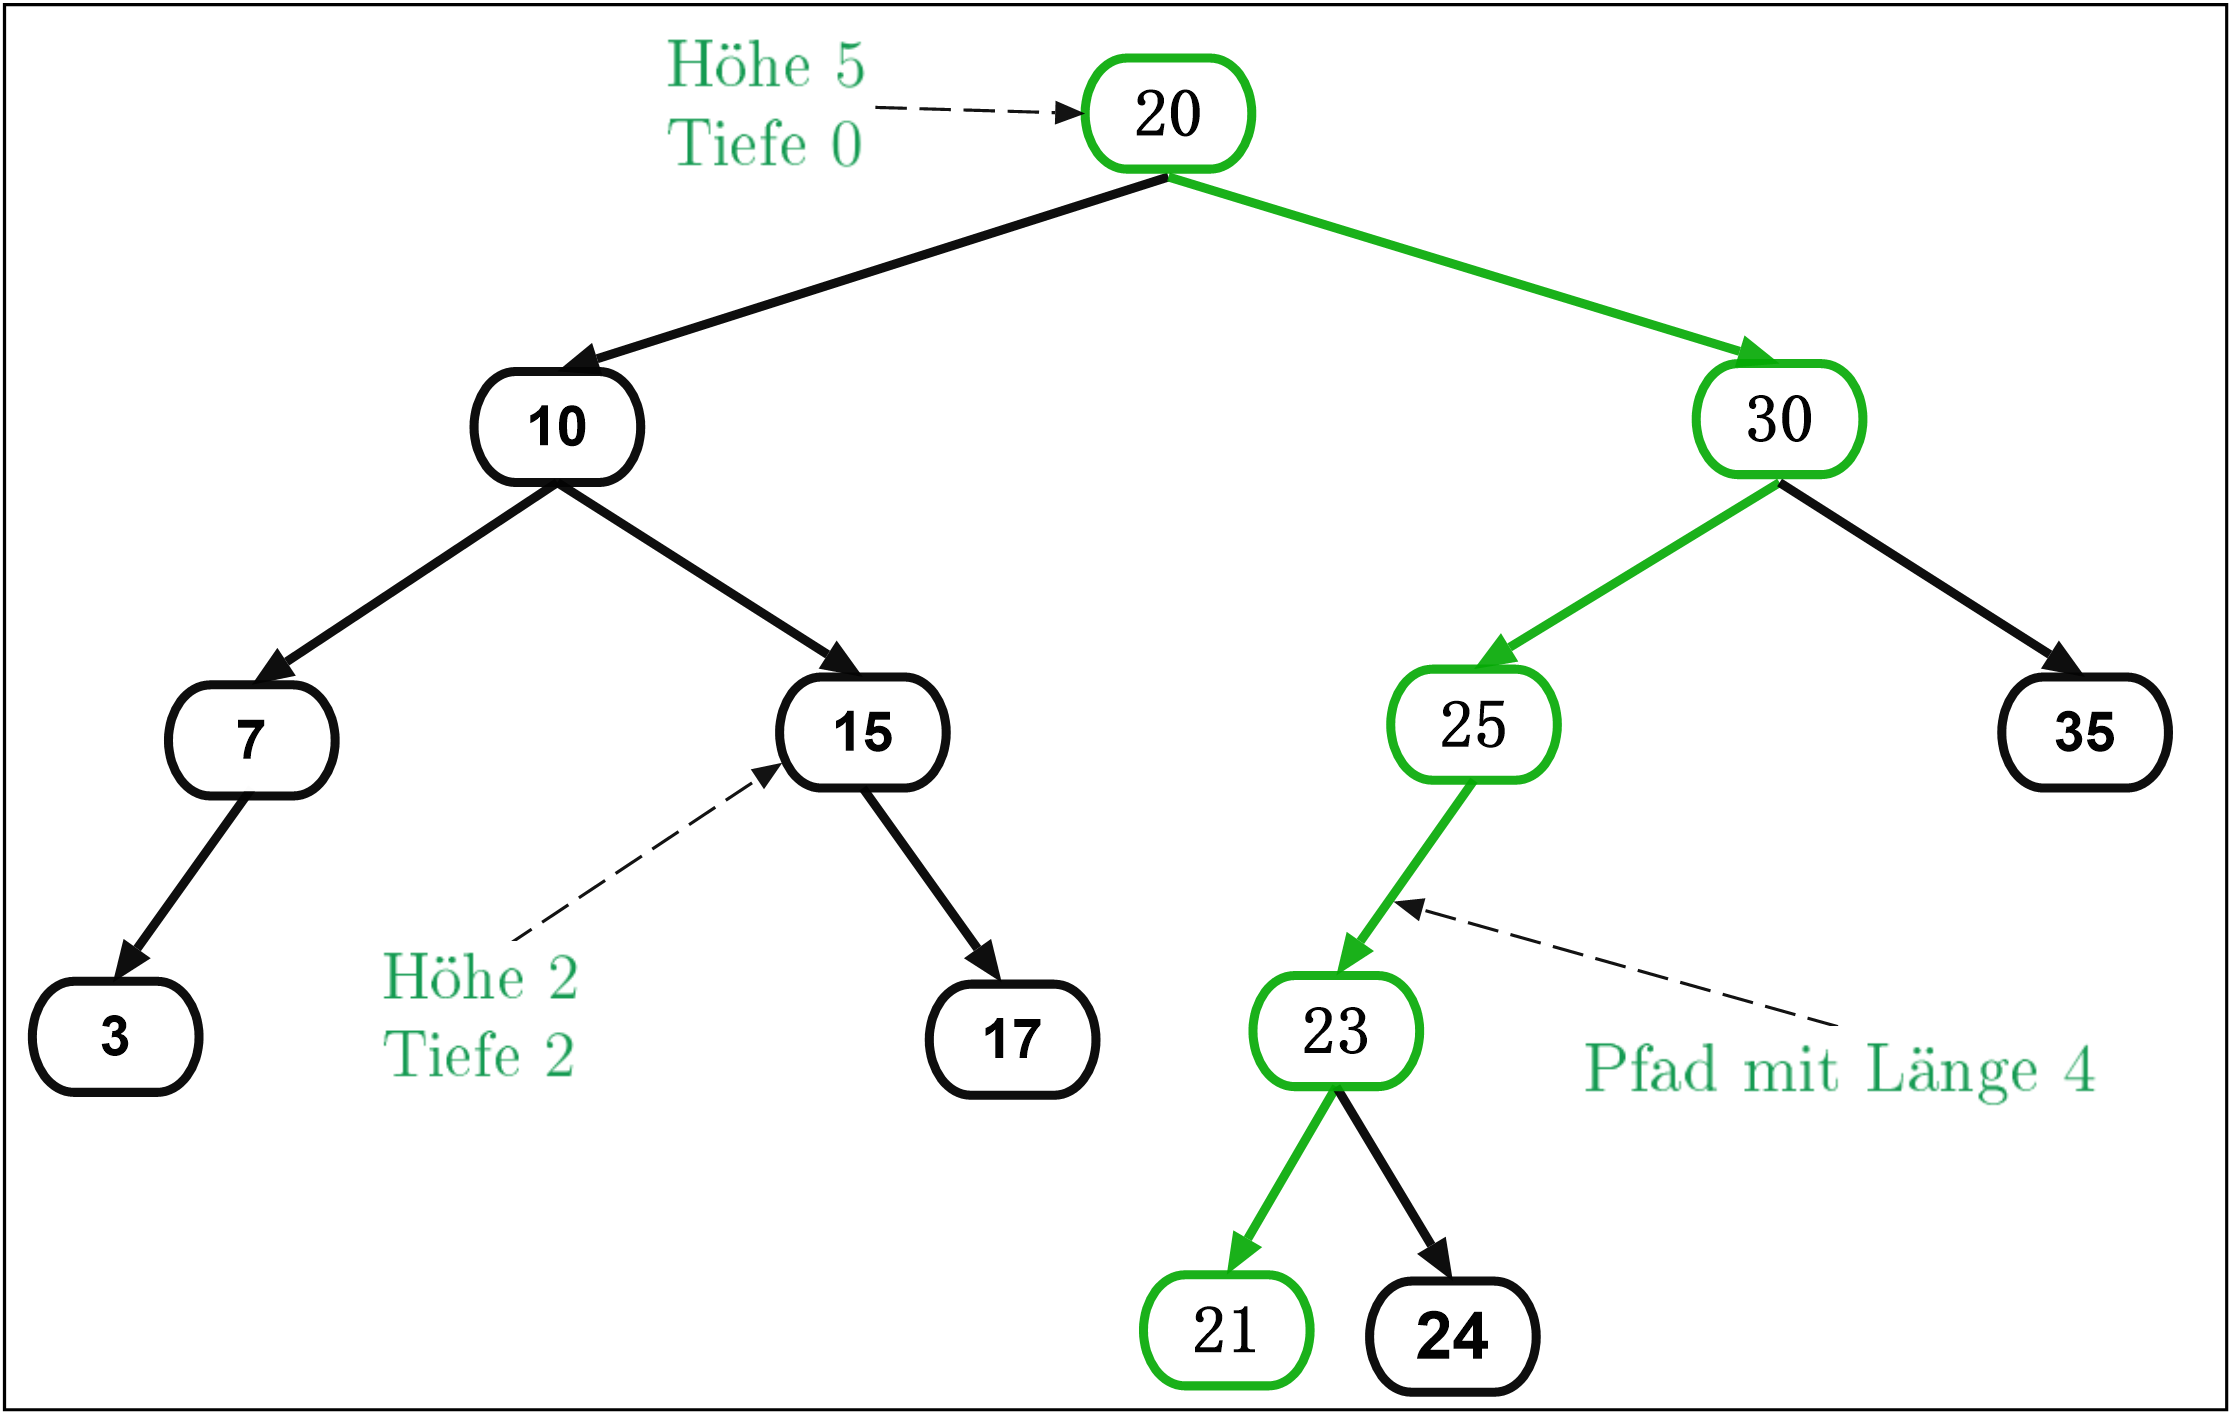
\includegraphics[width= 1\textwidth]{Medien/Einleitung/suchbaum2_2}
	\caption{Ein weiterer binärer Suchbaum }
	\label{fig:suchbaum2_2}
\end{figure}

\noindent Da im linken Teilbaum nur kleinere Schlüssel vorhanden sein dürfen und im rechten Teilbaum nur größere, kann die Schlüsselmenge eines binären Suchbaumes, von links nach rechts, in aufsteigend sortierter Form abgelesen werden. Aus Platzgründen passiert es bei Zeichnungen von BSTs manchmal, dass ein Knoten in einem linken Teilbaum weiter rechts liegt als die Wurzel dieses Teilbaumes oder umgekehrt, weshalb bei der Betrachtung solcher Zeichnungen etwas vorsichtig vorgegangen werden muss. Abbildung \ref{fig:linksRechts} enthält keine solche Konstellation.  

\begin{figure}[H]
	\centering
	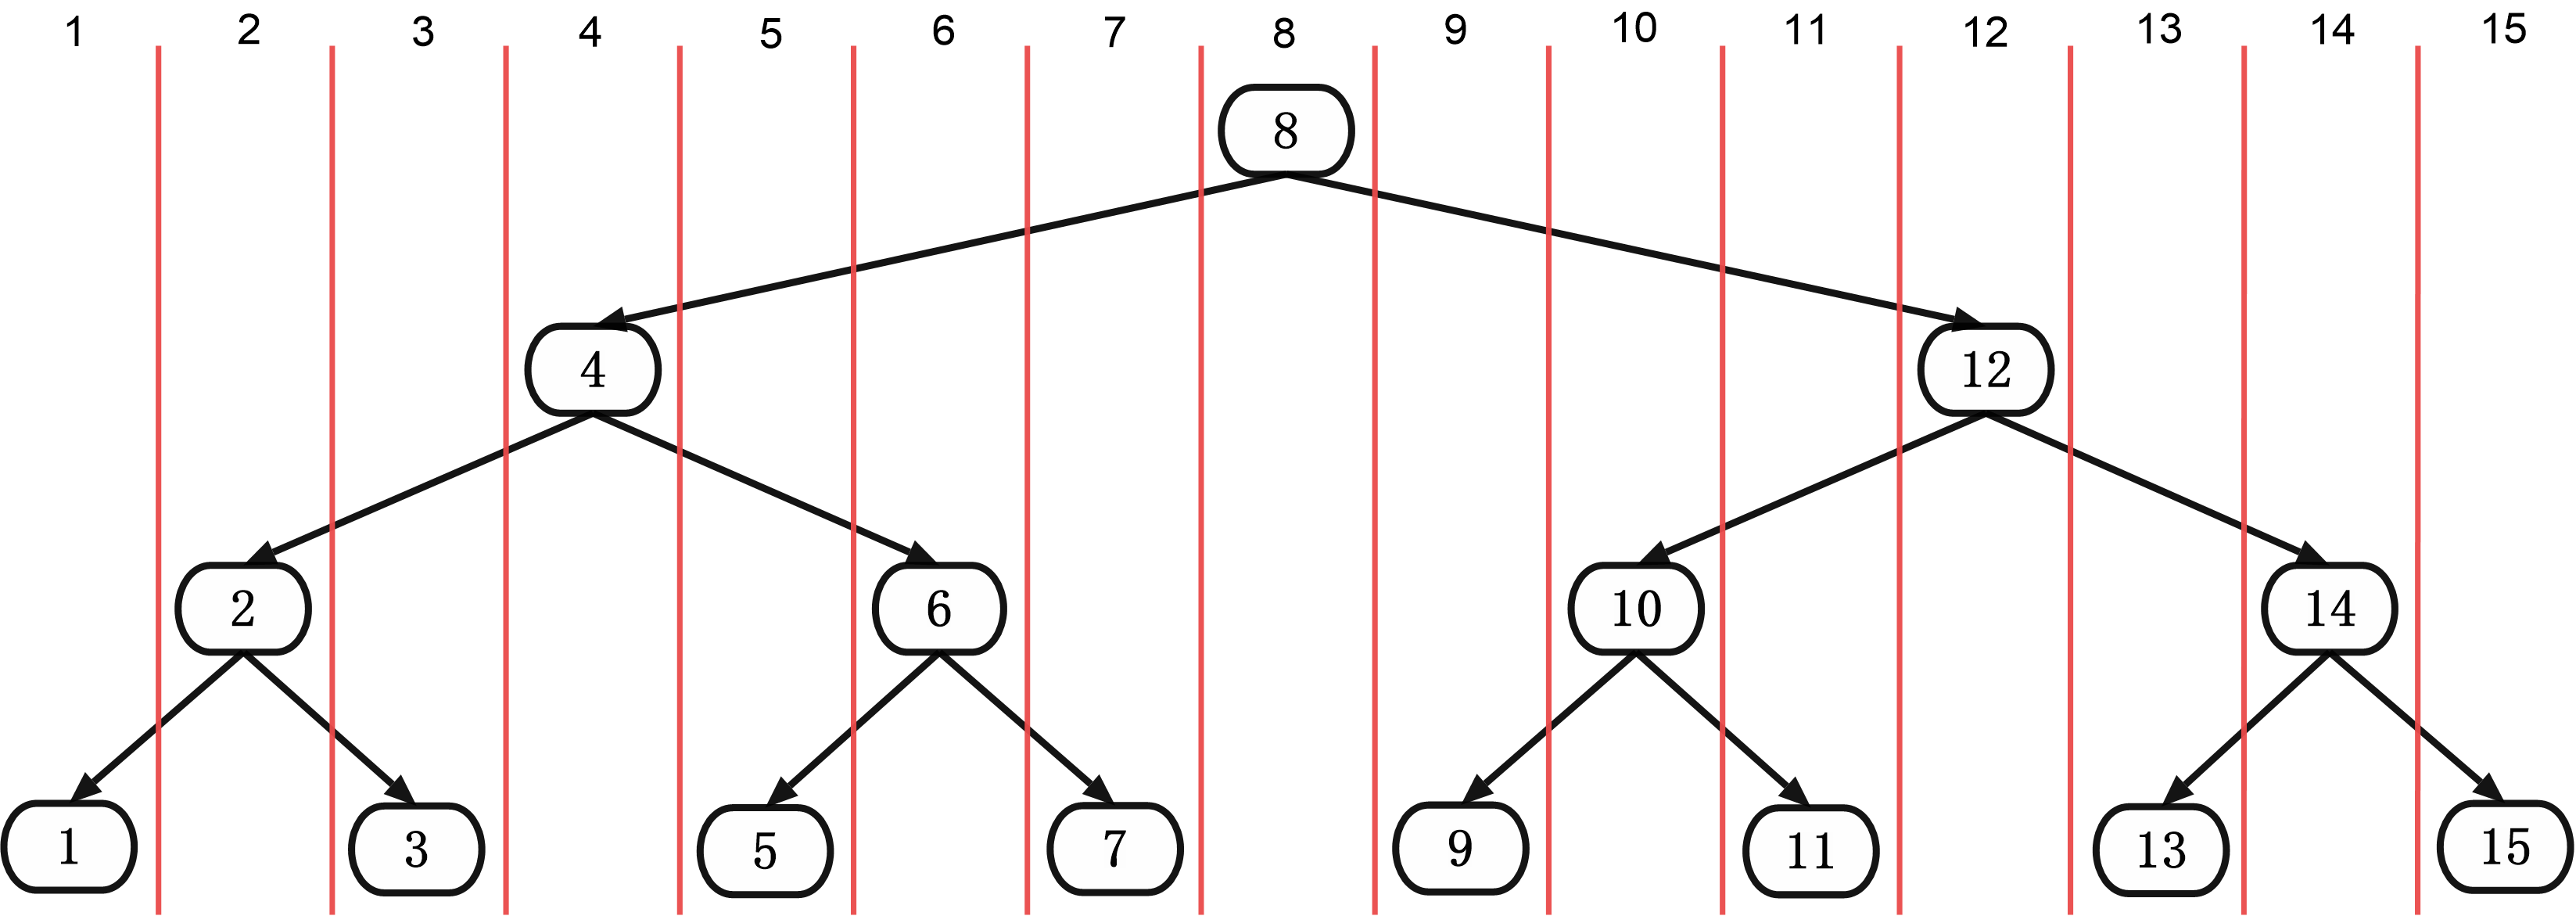
\includegraphics[width= 1\textwidth]{Medien/Einleitung/linksRechts}
	\caption{Die Schlüssel sind aufsteigend sortiert ablesbar. }
	\label{fig:linksRechts}
\end{figure}
\noindent Algorithmisch können die im BST enthaltenen Schlüssel aufsteigend sortiert durch eine \textbf{Inorder-Traversierung} ausgeben werden. Es ist ein rekursives Verfahren, das an der Wurzel startet und pro Aufruf drei Schritte ausführt:\\

Algorithmus \textit{inorder} $($Node $v)$
\begin{enumerate}
	\item Existiert das linke Kind $v_l$ von $v$, rufe \textit{inorder}$\left(v_l\right)$ auf. 
	\item Gib den Schlüssel von $v$ aus. 
	\item Existiert das rechte Kind $v_r$ von $v$, rufe  \textit{inorder}$\left(v_r\right)$  auf. 
\end{enumerate}

\noindent Dass das Verfahren funktioniert, wird sichtbar, durch Induktion über die Anzahl der Knoten $n$.
Für $n = 1$ funktioniert es, da der einzige im BST enthaltene Schlüssel ausgegeben wird. Wir nehmen nun an, dass die Ausgabe für BSTs mit Knotenzahl $\leq n$ korrekt ist. Sei $T_1$ ein BST mit der Knotenanzahl $n + 1$ und der Wurzel $w$. Sowohl für den linken, als auch für den rechten Teilbaum von $w$ gilt, dass die Anzahl der enthaltenen Knoten $\leq n$ ist. Als erstes wird der linke Teilbaum von $w$ korrekt ausgegeben, dann der Schlüssel von $w$ selbst und zuletzt der rechte Teilbaum von $w$. Damit wurde auch für den Gesamtbaum die richtige
Ausgabe erzeugt. \\
Als \textbf{Vorgänger} eines Knotens $v$ mit dem Schlüssel $k_v$ wird der Knoten mit dem größten im BST enthaltenen Schlüssel $k_p$, für den $k_p < k_v$ gilt, bezeichnet. Aus der Inorder-Traversierung kann eine Anleitung zum Finden des Vorgängers abgeleitet werden. Falls ein linker Teilbaum vorhanden ist, wird der größte Schlüssel in diesem, also der am weitesten rechts liegende, direkt vor $k_v$ ausgegeben. Ansonsten wird der Schlüssel des tiefsten Knotens auf dem Pfad von der Wurzel zu $v$ ausgegeben, bei dem $v$ im rechten Teilbaum liegt. \\
Als \textbf{Nachfolger} von $v$ wird der Knoten mit dem kleinsten im BST enthaltenen Schlüssel $k_s$, für den $k_s > k_v$ gilt, bezeichnet. Da dieser Schlüssel bei der Inorder-Traversierung direkt nach $v$ ausgegeben wird, ist der zugehörige Knoten ganz links im rechten Teilbaum von $v$ zu finden, falls ein solcher vorhanden ist. Ansonsten ist es der tiefste Knoten auf dem Pfad von der Wurzel zu $v$, bei dem $v$ im linken Teilbaum liegt. Abbildung \ref{fig:VorgängerNachfolger} zeigt den Vorgänger und den Nachfolger eines Knotens.\\
 Als \textbf{Vorfahre} eines Knotens $v$ werden alle Knoten auf dem Pfad von der Wurzel zu $v$, inklusive $v$ selbst, bezeichnet. 

\begin{figure}[H]
	\centering
	\includegraphics[width= 1\textwidth]{Medien/Einleitung/VorgängerNachfolger}
	\caption{Darstellung von Vorgänger und Nachfolger. }
	\label{fig:VorgängerNachfolger}
\end{figure}
\paragraph{Total geordnete Menge:} 
Eine Menge $M$ wird als \textbf{total geordnet} bezeichnet, wenn auf ihr eine zweistellige Relation $\leq$ definiert ist, die folgende Eigenschaften erfüllt.\\
Für alle $a$,$b$,$c$ $\in M$ gilt:
\begin{align*}
\text{1. } & (a,a) \in R  &\text{  (reflexiv)}\\
\text{2. } & (a,b) \in R  \land  (a,b) \in R \Rightarrow a = b  &\text{  (antisymmetrisch)}\\
\text{3. } & (a,b) \in R  \land  (b,c) \in R \Rightarrow  (a,c) \in R  &\text{  (transitiv)}\\
\text{4. } & (a,b) \notin R \Rightarrow  (b,a) \in R   &\text{  (total)}\\
\end{align*}
Die Eigenschaften 1,2 und 4 werden benötigt, um für zwei beliebige Elemente aus der Menge feststellen zu können, ob sie gleich sind oder bei Ungleichheit, welches Element weiter links, bzw. rechts im BST liegen muss. Dafür wird z.B. getestet, ob die Elemente $(a,b)$ und $(b, a)$ in der Relation liegen. Eigenschaft 3 ist notwendig. Denn liegt $b$ weiter rechts im BST als $a$ und $c$ liegt weiter rechts als $b$, dann liegt $c$ natürlich auch weiter rechts als $a$. \\
Die von uns verwendete \enquote{Kleiner-Gleich-Beziehung} auf den natürlichen Zahlen erfüllt alle Eigenschaften.
\\
\\




\paragraph{Verändern eines BSTs durch Rotationen:}
Wird ein BST durch eine Veränderung in einen anderen BST überführt, kann es passieren, dass sich die Eigenschaften eines Knotens ändern. Um nicht immer erwähnen zu müssen, auf welchen BST sich eine Aussage bezieht, wird es ab jetzt durchgängig so sein, dass sich ein Variablenname ohne angefügten Hochstrich auf den BST vor der Änderung bezieht. Der gleiche Variablenname mit angefügtem Hochstrich bezieht sich dann auf den selben Knoten nach der Änderung. Beispielsweise bezieht sich $x$ auf den Knoten mit dem Schlüssel $k$ in der Ausgangssituation, dann bezieht sich $x'$ auf den Knoten mit dem Schlüssel $k$ nach dem Ausführen der Änderung. \\

\noindent\textbf{Rotationen:} können verwendet werden, um lokale Änderungen an der Struktur eines BSTs durchzuführen, ohne eine der geforderten Eigenschaften zu verletzen. Es wird zwischen der \textbf{Linksrotation} und der \textbf{Rechtsrotation} unterschieden. Hier wird zunächst auf die in Abbildung \ref{fig:Linksrotation} dargestellte Linksrotation eingegangen. 
Sei $x$ der Knoten auf dem eine Linksrotation durchgeführt wird. Sei $z$ der Elternknoten von $x$. $z$ muss existieren, ansonsten darf auf $x$ keine Rotation durchgeführt werden. Sei $B$ der linke Teilbaum von $x$. Nach der Rotation ist $x'$ das linke, bzw. rechte Kind von dem Knoten, von dem $z$ das linke, bzw. rechte Kind war. $z'$ ist das linke Kind von $x'$. Die Wurzel von $B '$ ist das rechte Kind von $z'$. Unabhängig von der Anzahl der im BST enthaltenen Knoten und der Ausführungsstelle im BST ist eine Linksrotation daher mit dem Aufwand verbunden, maximal drei Zeiger umzusetzen. Abbildung \ref{fig:Rechtsrotation} zeigt die symmetrische Rechtsrotation. Dass es durch eine Rotation zu keiner Verletzung der BST Eigenschaften kommt, kann den Abbildungen direkt entnommen werden. In Abbildung \ref{fig:LinksRechtsRotation} ist zu erkennen, dass sich die Wirkung einer Rotation auf $x$ durch eine gegenläufige Rotation auf $z'$ aufheben lässt.  
\begin{figure}[H]
	\centering
	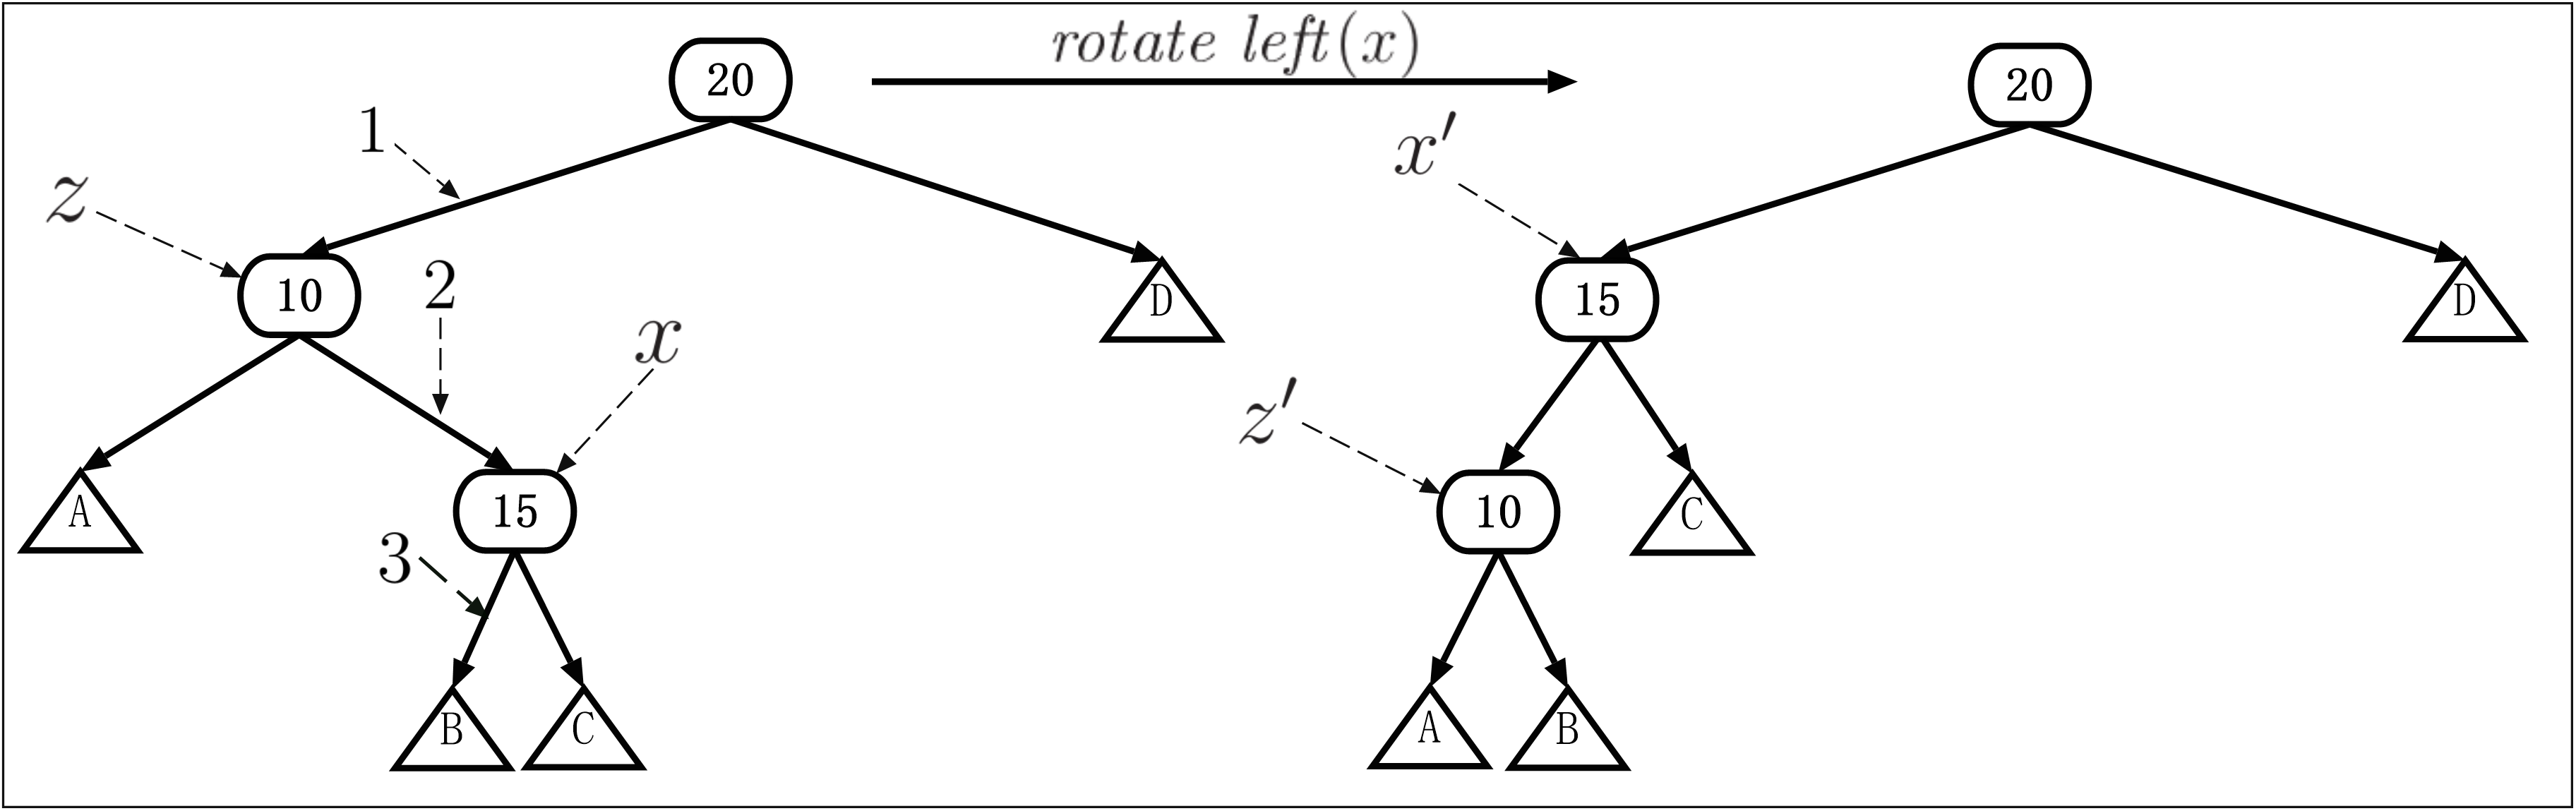
\includegraphics[width= 1\textwidth]{Medien/Einleitung/Linksrotation}
	\caption{Linksrotation auf Knoten x. }
	\label{fig:Linksrotation}
\end{figure}
\begin{figure}[H]
	\centering
	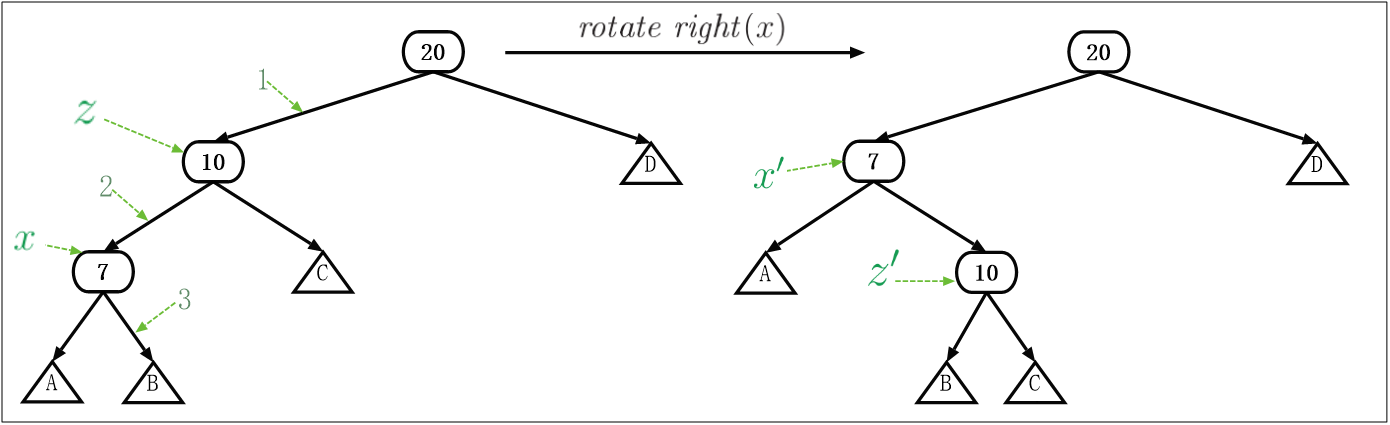
\includegraphics[width= 1\textwidth]{Medien/Einleitung/Rechtsrotation}
	\caption{Rechtsrotation auf Knoten x. }
	\label{fig:Rechtsrotation}
\end{figure}
\begin{figure}[H]
	\centering
	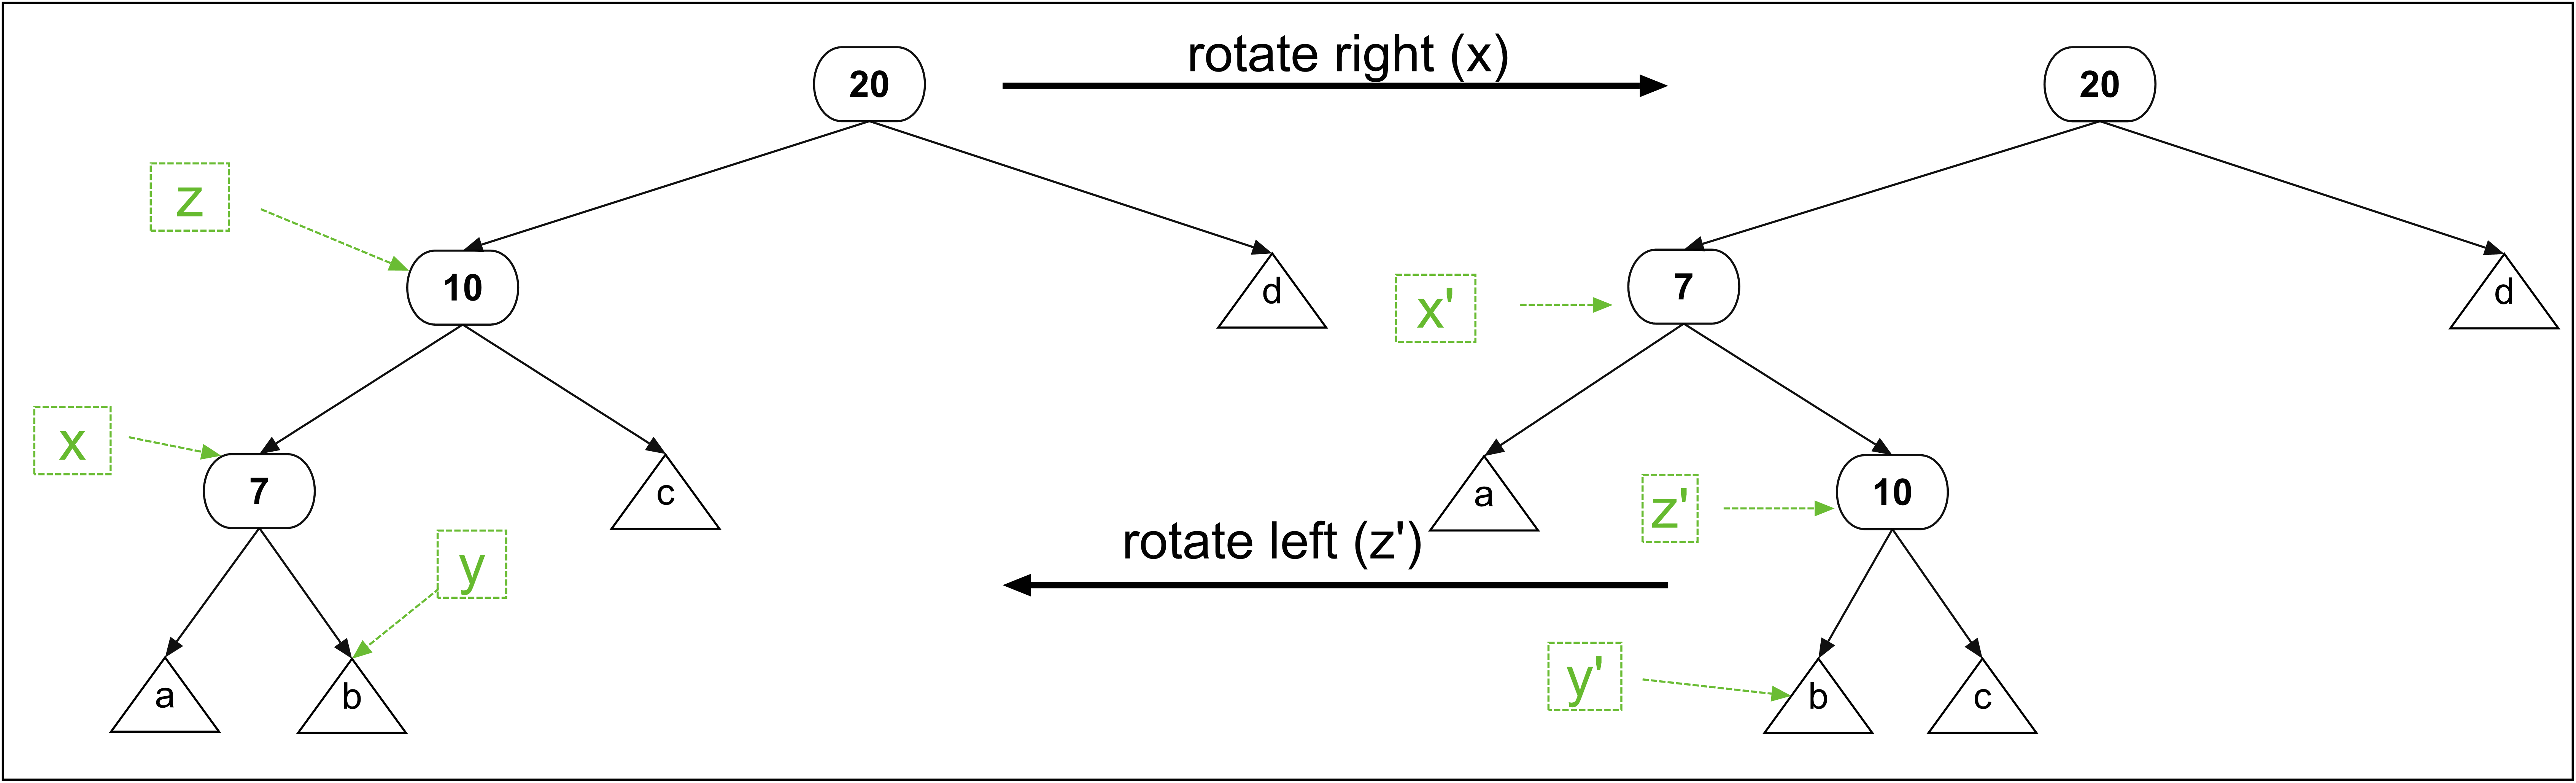
\includegraphics[width= 1\textwidth]{Medien/Einleitung/LinksRechtsRotation}
	\caption{Gegenseitiges Aufheben von Rotationen.}
	\label{fig:LinksRechtsRotation}
\end{figure}

\subsection{Die Grundoperationen \textit{search}, \textit{insert} und \textit{delete}.} \label{BST Operationen}
Hier werden nur die Standardvarianten eines BSTs gezeigt. Später werden Varianten gezeigt, die von diesem Verhalten zum Teil deutlich abweichen. Innerhalb von Operationen wird häufig von einem Knoten aus direkt
auf dessen Elternknoten zugegriffen, so dass sich im Baum auch nach oben hin bewegt werden kann. In Implementierungen wird das so umgesetzt, dass es zusätzlich zu den beiden Zeigern auf die Kinder noch einen zum Elternknoten gibt. Innerhalb eines Pfades werden in dieser Arbeit jedoch entweder nur Zeiger auf Kinder oder nur auf Elternknoten verwendet.\\
 Es sei ein BST $T$ gegeben. Die Operation \textit{search}$($key $k)$ gibt eine Referenz auf den Knoten im BST zurück, dessen Schlüssel mit $k$ übereinstimmt. Die Operation startet an der Wurzel und vergleicht den darin enthaltenen Schlüssel mit dem Gesuchten. Ist der gesuchte Schlüssel kleiner, muss er sich im linken Teilbaum des betrachteten Knotens befinden und die Suche wird bei dessen Wurzel fortgesetzt. Ist der Schlüssel größer, muss er sich im rechten Teilbaum befinden und die Suche wird bei dessen Wurzel fortgesetzt. Dieses Verhalten iteriert solange, bis der gesuchte Schlüssel gefunden ist oder der Teilbaum bei dem die Suche fortgesetzt werden müsste, leer ist. Ist das Letztere der Fall, ist der gesuchte Schlüssel im Baum nicht vorhanden und es wird eine leere Referenz zurückgegeben. In keinem Fall kommt es zu einer Veränderung des BST.\\
Mit \textit{insert}$($key $k)$  kann eine Schlüsselmenge um den Schlüssel $k$ erweitert werden. 
Bei \textit{insert}$($key $k)$  wird sich zunächst wie bei  \textit{search}$($key $k)$ verhalten. Wird $k$ gefunden, wird die Operation abgebrochen und der BST bleibt unverändert. Wird ein leerer Teilbaum $T_2$ erreicht, wird ein neu erzeugter Knoten mit dem Schlüssel $k$ an der Position von $T_2$ eingefügt. Durch den neuen Knoten wird keine BST Eigenschaft verletzt. Durch Ersetzen eines leeren Teilbaumes durch einen Knoten bleibt es bei einem binären Baum. Das Verhalten von  \textit{insert} stellt sicher, dass $k$ nur in linken Teilbäumen von Knoten mit einem Schlüssel $> k$, bzw. in rechten Teilbäumen von Knoten mit einem Schlüssel~ $< k$ enthalten ist.    \\
\begin{figure}[H]
	\centering
	\includegraphics[width= 1\textwidth]{Medien/Einleitung/SuchenEinfügen}
	\caption{Links zeigt eine Suche nach dem Schlüssel 15. Rechts das Einfügen des Schlüssels 13.}
	\label{fig:SuchenEinfügen}
\end{figure}
\noindent Auch bei \textit{delete}$($key $k)$ wird sich zunächst wie bei  \textit{search}$($key $k)$ verhalten. Ist $k$ im BST nicht vorhanden, wird abgebrochen und der BST bleibt unverändert. Ansonsten werden drei Fälle unterschieden.
Sei $v$ der Knoten mit dem Schlüssel $k$.
\begin{enumerate}
	\item $v$ ist ein Blatt: \\
	$v$ kann ohne weiteres aus dem BST entfernt werden.
	\item $v$ hat genau ein Kind $c$:\\
	Ist $v$ die Wurzel kann er entfernt werden und $c$ wird zur neuen Wurzel. Ansonsten ist $v$ entweder das linke oder das rechte Kind eines Knotens $w$. $c$ nimmt nun den Platz von $v$ im BST ein. Das bedeutet, dass die Kanten von $w$ nach $v$ und von $v$ nach $c$ entfernt werden. Außerdem wird eine Kante von $w$ nach $c$ so eingefügt, dass $c$ wie zuvor $v$, das linke, bzw. rechte Kind von $w$ wird. 
	\item $v$ hat zwei Kinder:\\
	Sei $T_l$ der linke Teilbaum von $v$ und $T_r$ der Rechte.
	Sei $z$ der Knoten mit dem kleinsten Schlüssel im rechten Teilbaum von $v$. Als Knoten mit dem kleinsten Schlüssel im rechten Teilbaum von $v$, kann $z$ kein linkes Kind haben. Ist $z$ ein Blatt wird seine eingehende Kante entfernt. Hat $z$ ein rechtes Kind $z_r$, so nimmt dieses, analog zur Beschreibung im Fall 2, den Platz von $z$ ein. In beiden Fällen ist $z$ nun ein Knoten ohne Kante. Im nächsten Schritt nimmt nun $z$ den Platz von $v$ ein. $T_l$ wird links an $z$ angefügt und $T_r$ rechts. War $v$ zu Beginn die Wurzel, so wird $z'$ zur neuen Wurzel.\\
	In keinen Teilbäumen eines Knotens außer denen von $z$ kommen Schlüssel hinzu. Um eventuelle Verletzungen von Eigenschaften festzustellen, kann sich also auf $z'$ beschränkt werden. Der linke Teilbaum von $z'$ war der linke Teilbaum von $v$ und der Schlüssel von $v$ ist kleiner als der von $z$. Der rechte Teilbaum von $z$ enthält die Schlüssel des rechten Teilbaumes von $v$ mit Ausnahme des Schlüssels von $z$ selbst. $z$ wurde gerade ausgewählt weil sein Schlüssel der Kleinste in diesem Teilbaum ist. 
	
	
	
	
\end{enumerate} 
\begin{figure}[H]
	\centering
	\includegraphics[width= 1\textwidth]{Medien/Einleitung/löschen}
	\caption{Löschen des Schlüssels 10}
	\label{fig:löschen}
\end{figure}
\paragraph{Laufzeit:}
Die Laufzeit der drei Operationen ist jeweils $\mathit{O(h)}$, wobei $h$ die Höhe von $T$ ist. Bei \textit{search} werden maximal $h$ Knoten aus $T$ betrachtet. Beim Einfügen überlagern die Kosten der Suche, die konstanten Kosten für das Einbinden des neuen Knotens. Bei \textit{delete} wird in Fall eins und zwei nach dem Suchen ebenfalls nur noch lokal beim gesuchten Knoten gearbeitet. Bei \textit{delete} mit Fall drei muss zunächst der Knoten $z$ erreicht werden. Dafür sind maximal $h$ Schritte notwendig. Danach muss $v$ erreicht werden, wozu ebenfalls maximal $h$ Schritte notwendig sind. Die Kosten für das Entfernen und Hinzufügen von Kanten sind an beiden Stellen konstant.  



\paragraph{Unterschiedliche Baumhöhen:}
Da die Höhe $h$ eines BST $T$ mit $n$ Knoten entscheidend für die Laufzeit der vorgestellten Operationen ist, wird hier auf diese eingegangen. Die maximale Höhe $n$ erreicht ein BST, wenn es genau ein Blatt im BST gibt und jeder andere Knoten genau ein Kind hat. Die Baumstruktur geht in diesem Fall zu einer Listenstruktur über. Dies wird als \textbf{entarten} bezeichnet. Minimal wird $h$, wenn $T$ \textbf{vollständig balanciert} ist. Das ist der Fall, wenn alle Ebenen über der Untersten vollständig besetzt sind. Sind zusätzlich in der untersten Ebene, links von jedem Knoten, alle Knoten enthalten, wird der BST als \textbf{komplett} bezeichnet, siehe \mbox{Abbildung \ref{fig:kompletterBaum}}. 
\begin{figure}[H]
	\centering
	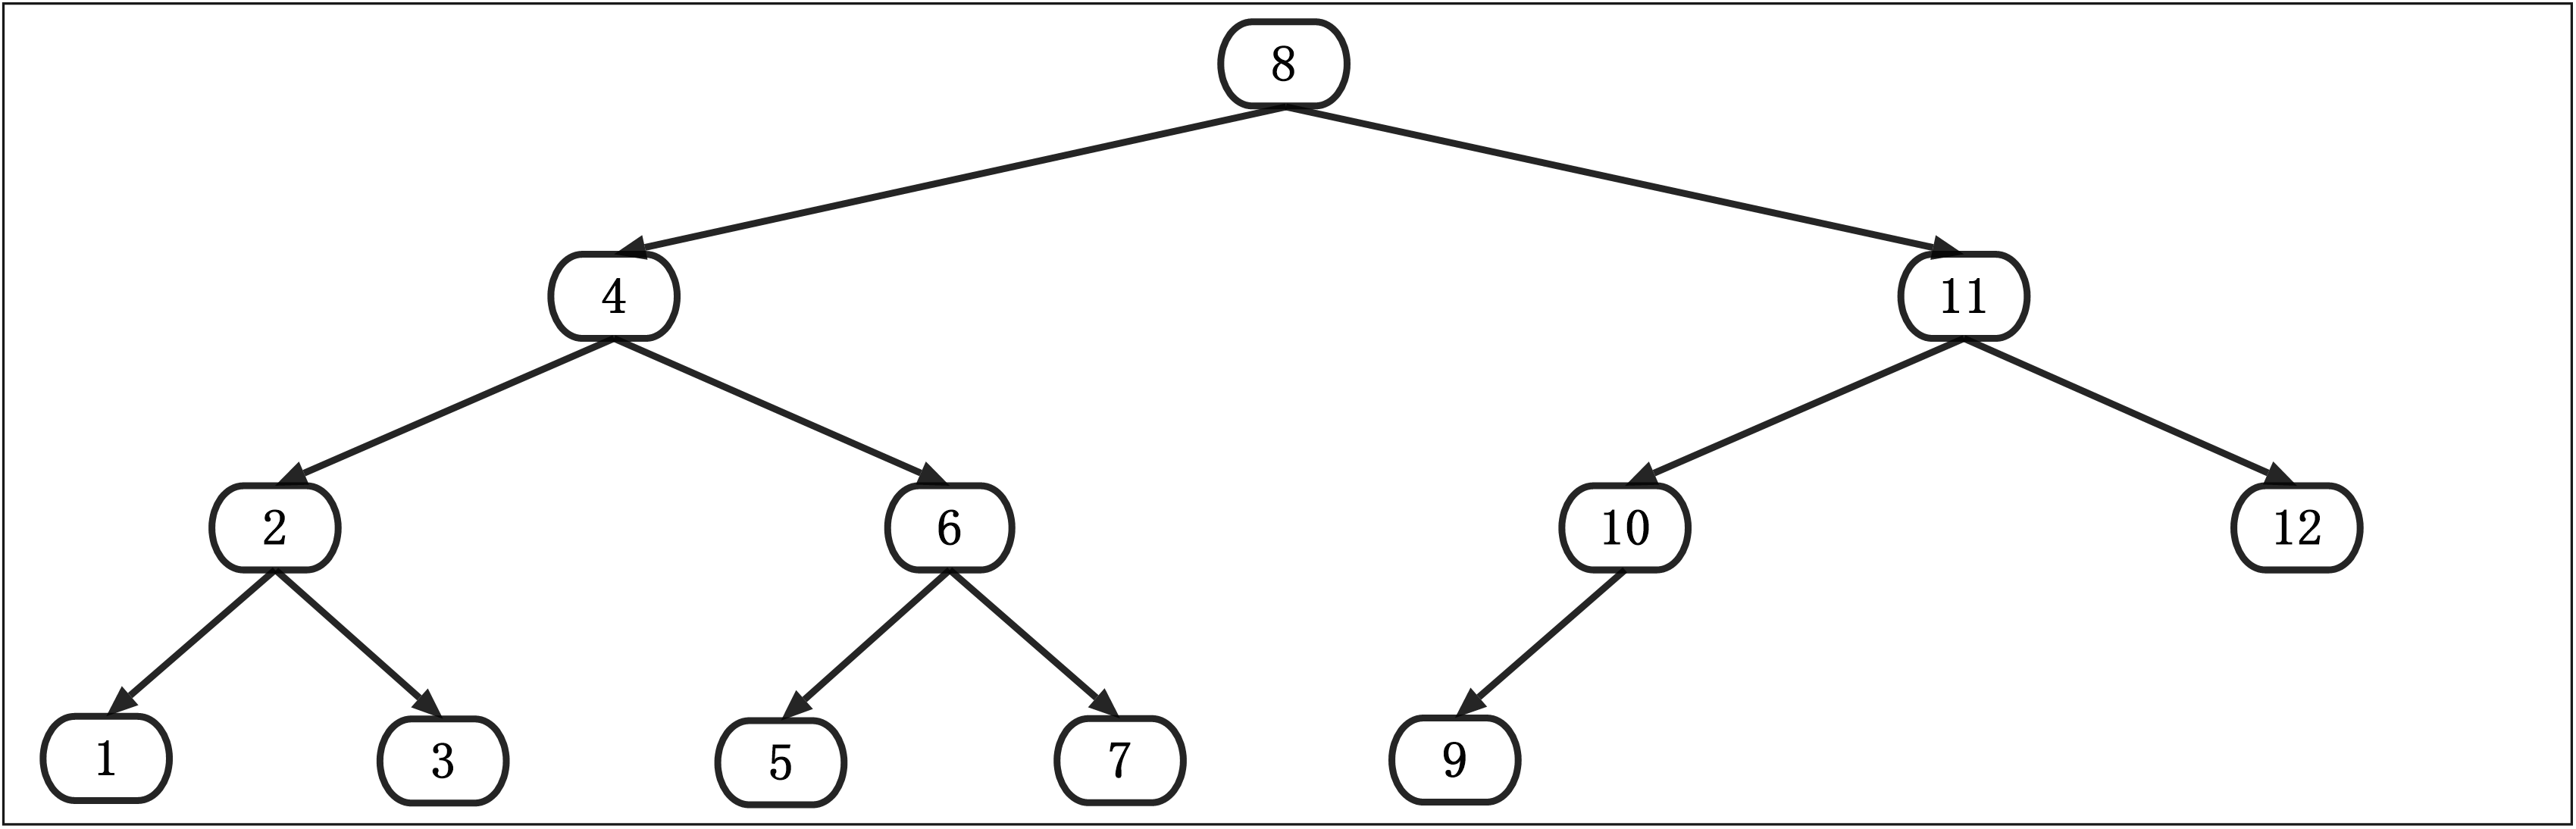
\includegraphics[width= 1\textwidth]{Medien/Einleitung/kompletterBaum}
	\caption{Kompletter BST mit 12 Knoten}
	\label{fig:kompletterBaum}
\end{figure}


\begin{Lemma} Die Höhe eines vollständig balancierten BSTs $T$ mit $n$ Knoten ist $ \lfloor \log_2{(n)} \rfloor + 1 $. 
\end{Lemma}
\begin{proof}
	
	Es sei $\mathit{N(h)}$ die maximale Anzahl an Knoten in einem vollständig balancierten BST mit Höhe $h$.
	$\mathit{N(h)}$  berechnet sich, indem die Summe der maximalen Anzahl an Knoten jeder Ebene gebildet wird.\\
	\begin{align*}
	\mathit{N(h)} = \sum\limits_{i=0}^{h-1} 2^i = 2^h - 1 
	\end{align*}
	
	\noindent	$h$ ist minimal, wenn gilt:\\
	\begin{align*}
	\mathit{N(h-1)} &< n \leq \mathit{N(h)}\\
	\Leftrightarrow \mathit{N(h-1)} + 1 &\leq n < \mathit{N(h)} + 1\\
	\end{align*}
	Einsetzen:\\
	\begin{align*}
	&2^{h - 1} \leq n < 2^h\\
	\Rightarrow & h =  \lfloor \log_2{(n)} \rfloor + 1
	\end{align*}
	
\end{proof}
\section{Rot-Schwarz-Baum}
Der Tango Baum besteht intern aus Hilfsbäumen. Der Rot-Schwarz-Baum gehört zur Gruppe der \textbf{balancierten BST} und erfüllt alle Eigenschaften, um ihn als Hilfsbaum im Tango Baum verwenden zu können. Genau das ist auch die Rolle des Rot-Schwarz-Baumes in dieser Ausarbeitung. Bei balancierten BSTs gilt für die Höhe $h = \mathit{O(\log\left( n\right))}$, mit $n =$ Anzahl der Knoten. Jeder Knoten benötigt ein zusätzliches Attribut, um eine Farbinformation zu speichern. Der Name der Datenstruktur kommt daher, dass die beiden durch das zusätzliche Attribut unterschiedenen Zustände als \textit{rot} und \textit{schwarz} bezeichnet werden. Die Farbe ist also eine Eigenschaft der Knoten und im Folgendem wird einfach von roten, bzw. schwarzen Knoten gesprochen. Als Blätter werden schwarze Sonderknoten verwendet, deren Schlüssel auf einen Wert außerhalb des Universums, hier \textit{null}, gesetzt wird, um sie eindeutig erkennen zu können. $\mathit{null}$ gehört nicht zur Schlüsselmenge des  Rot-Schwarz-Baumes. Fehlende Kinder von Knoten mit einem gewöhnlichen Schlüssel werden durch solche Blätter ersetzt.  

\noindent Folgende zusätzliche Eigenschaften müssen bei einem Rot-Schwarz-Baum erfüllt sein. 

\begin{enumerate}
	\item Jeder Knoten ist entweder rot oder schwarz.
	\item Die Wurzel ist schwarz.
	\item Jedes Blatt (Sonderknoten) ist schwarz.
	\item Der Elternknoten eines roten Knotens ist schwarz.
	\item Für jeden Knoten gilt, dass alle Pfade, die an ihm starten und an einem Blatt (Sonderknoten) enden, die gleiche Anzahl an schwarzen Knoten enthalten. 
\end{enumerate}  
Sei $(v_0,v_1,...,v_n)$ ein Pfad von einem Knoten $v_0$ zu einem Blatt $v_n$. Die Anzahl der schwarzen Knoten innerhalb $(v_1,...,v_n)$ wird als \textbf{Schwarz-Höhe} $\mathit{bh(v_0)}$ von Knoten $v_0$ bezeichnet. Die eigene Farbe des betrachteten Knotens bleibt dabei also außen vor. Dadurch hat ein Knoten die gleiche Schwarz-Höhe wie ein rotes Kind von ihm und eine um eins erhöhte Schwarz-Höhe gegenüber einem schwarzen Kind. Die Schwarz-Höhe der Wurzel entspricht der \textbf{Schwarz-Höhe des Baumes~ $bh(T)$}, wobei ein leerer Baum die Schwarz-Höhe $0$ hat. Die Schwarz-Höhe eines Knotens $x$ ist genau dann eindeutig, wenn er die Eigenschaft 5 nicht verletzt. Hält $x$ die Eigenschaft 5 ein und sei $i$ die Anzahl schwarzer Knoten in den entsprechenden Pfaden, so gilt $\mathit{bh(x)} = i$, wenn $x$ rot ist und $\mathit{bh(x)} = i - 1$, wenn $x$ schwarz ist. Ist $\mathit{bh(x)}$ eindeutig, so enthält jeder Pfad, der mit $x$ startet und an einem Blatt endet, $\mathit{bh(x)} + 1$ schwarze Knoten, wenn $x$ schwarz ist und  $\mathit{bh(x)}$ schwarze Knoten, wenn $x$ rot ist.\\ Jeder Knoten speichert seine Schwarz-Höhe als weiteres Attribut, da wir dieses in Abschnitt \ref{vereinigen} benötigen. Natürlich muss das Attribut dann auch gesetzt und gepflegt werden, wobei es bei Sonderknoten fest mit $0$ belegt ist. Im Folgenden wird \textbf{RBT} (Red Black Tree) als Abkürzung für Rot-Schwarz-Baum verwendet. Aufgrund der Sonderknoten gibt es eine etwas spezielle Situation bei einem RBT mit Höhe 1. Diese Konstellation ist nur mit einem einzelnen Sonderknoten erreichbar, so dass statt dessen auch einfach der leere Baum verwendet werden könnte. Auch diese Konstellation erfüllt aber die fünf Eigenschaften, so dass sie kein Problem darstellt. \\



\begin{figure}[H]
	\centering
	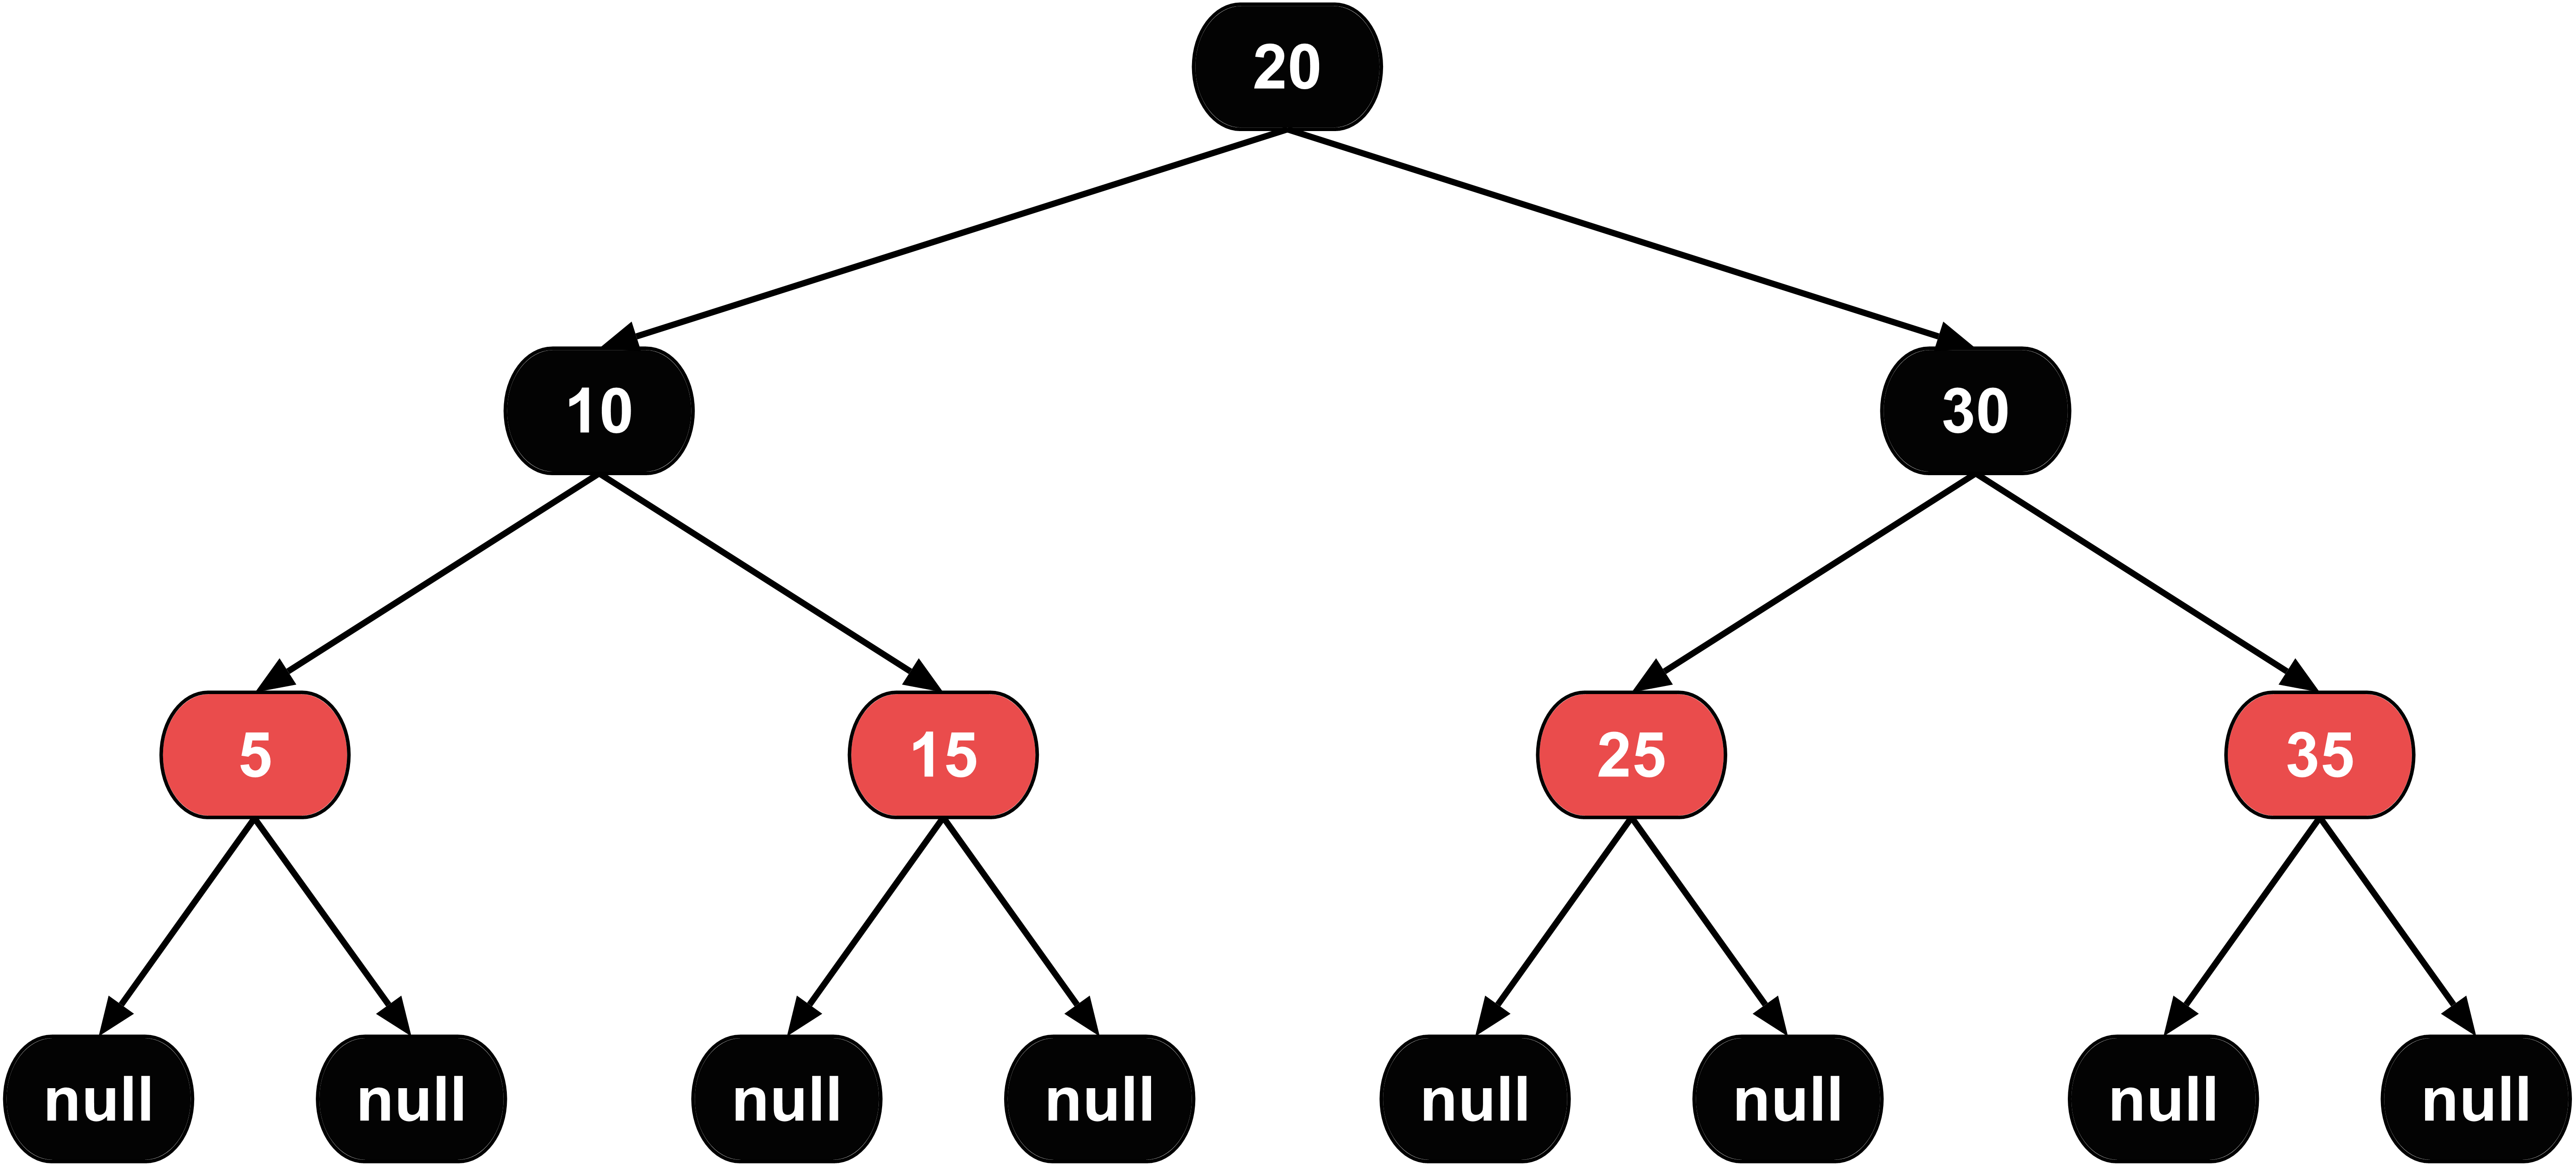
\includegraphics[width= 1\textwidth]{Medien/RotSchwarzBaum/IOBaum}
	\caption{RBT ohne Verletzung von Eigenschaften. }
	\label{fig:IOBaum}
\end{figure}
\begin{figure}[H]
	\centering
	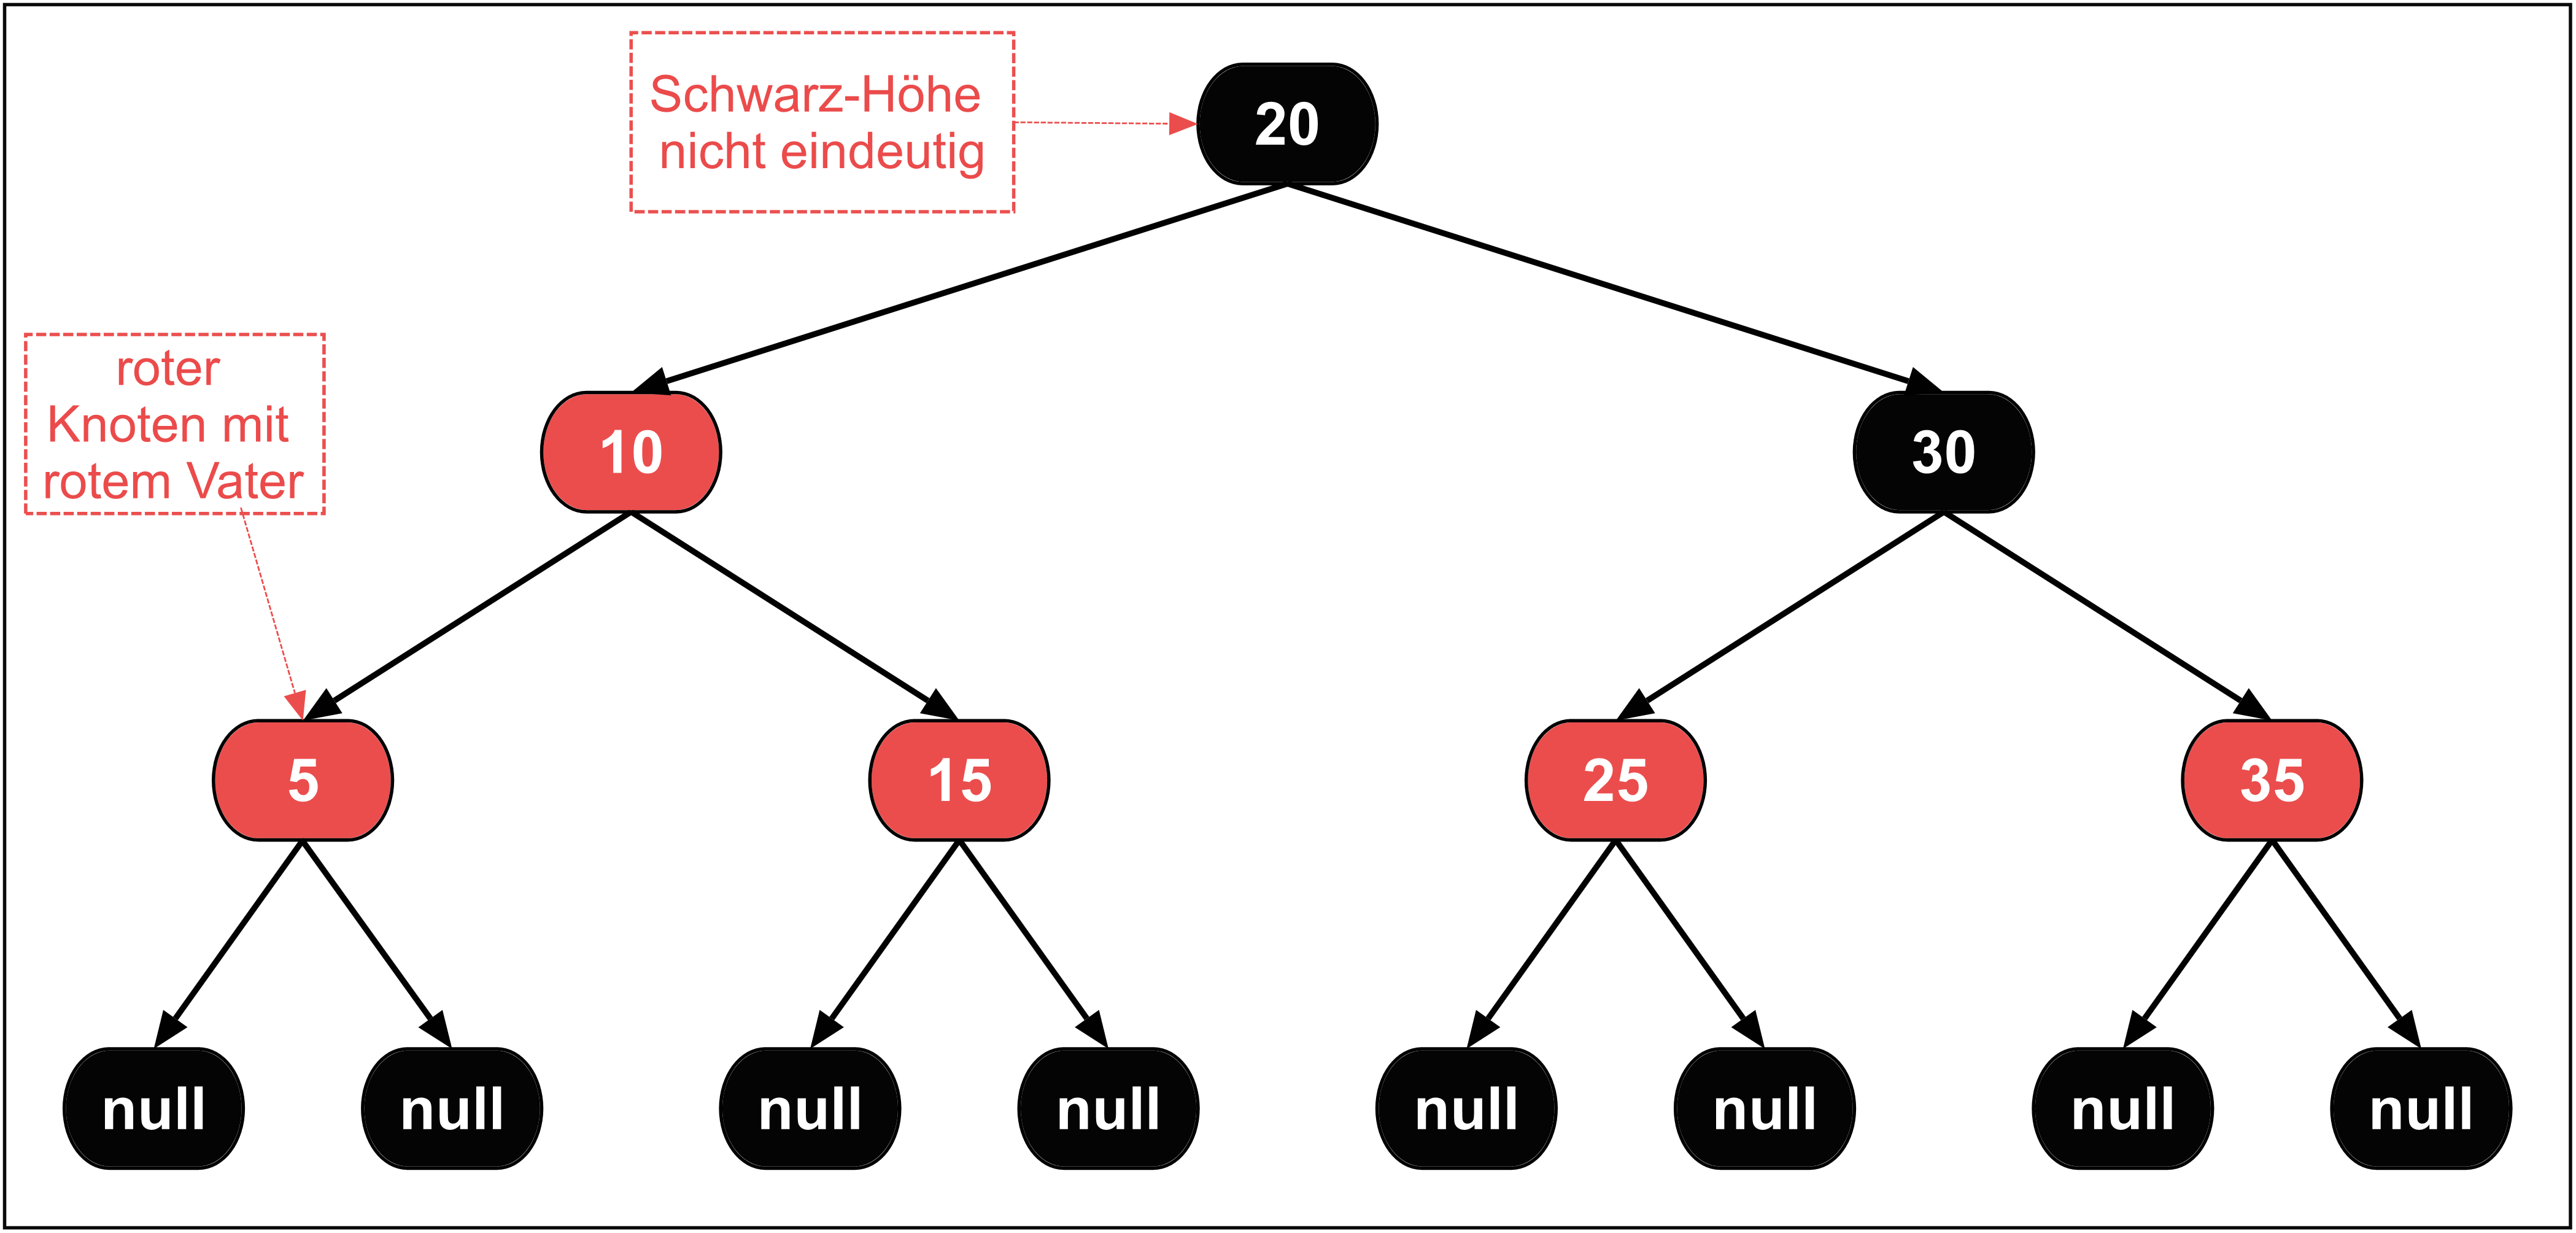
\includegraphics[width= 1\textwidth]{Medien/RotSchwarzBaum/NIOBaumZweiRote}
	\caption{Kein RBT, da die Eigenschaften vier und fünf verletzt sind. }
	\label{fig:NIOBaumZweiRote}
\end{figure}
\begin{figure}[H]
	\centering
	\includegraphics[width= 1\textwidth]{Medien/RotSchwarzBaum/NIOBaumPfadlänge}
	\caption{Kein RBT, da die Eigenschaft fünf verletzt ist.  }
	\label{fig:NIOBaumPfadlänge}
\end{figure}
\subsection{Grundoperationen}
\paragraph{Suchen im Rot-Schwarz-Baum:}
Die Suche unterscheidet sich nur in einem Punkt von der in Abschnitt \ref{BST Operationen} vorgestellten. Wird nach einem Schlüssel gesucht, der im RBT nicht vorhanden ist, so wird einer der Sonderknoten erreicht. In diesem Fall wird die Suche abgebrochen und eine leere Referenz zurückgegeben. Die Operation verändert den RBT nicht. 

\paragraph{Einfügen in den Rot-Schwarz-Baum:}
\textit{insert} wird für einen Hilfsbaum im Tango Baum eigentlich nicht benötigt. Im Kapitel zum Tango Baum wird später jedoch eine Hilfsoperation benötigt, die am besten zu \textit{insert} beschrieben werden kann.\\
Sei $k$ der einzufügende Schlüssel. Zunächst wird wie beim Suchen vorgegangen. Wird $k$ gefunden, wird der RBT nicht verändert. Ansonsten wird ein Sonderknoten $b$ erreicht (Annahme der RBT ist nicht leer). Ein neu erzeugter roter Knoten $v_k$ mit dem Schlüssel $k$ und Schwarz-Höhe $1$ nimmt den Platz von $b$ ein. $k$ werden Sonderknoten als linkes und rechtes Kind angefügt. $k$ ist nun im Baum enthalten. Es muss jedoch auf mögliche Verletzungen der fünf Eigenschaften geachtet werden. Welche können betroffen sein ?

\begin{enumerate}
	\item Es ist immer noch jeder Knoten entweder rot oder schwarz.
	\item Wurde in einen RBT mit leerer Schlüsselmenge eingefügt, so ist der neu erzeugte rote Knoten die Wurzel, was eine Verletzung darstellt. Waren bereits Schlüssel im Baum vorhanden blieb die Wurzel unverändert.
	\item Aufgrund der Sonderknoten sind die Blätter immer noch schwarz.
	\item Der Baum wird nur direkt an der Einfügestelle verändert, so dass nur $v_k$ betrachtet werden muss. $v_k$ hat schwarze Kindknoten. Er könnte jedoch einen roten Elternknoten haben, so dass diese Eigenschaft verletzt wäre.
	\item Die Schwarz-Höhe von $v_k$ ist korrekt gesetzt. Waren bereits Knoten im RBT vorhanden, so kann sich ihre Schwarz-Höhe nicht verändert haben, denn den Platz eines schwarzen Knotens mit Schwarz-Höhe $0$ nimmt dann ein roter Knoten mit Schwarz-Höhe $1$ ein. Eigenschaft fünf bleibt also erhalten. 
\end{enumerate}  

\noindent Es können also die Eigenschaften zwei und vier betroffen sein. Jedoch nur eine von ihnen, denn Eigenschaft zwei wird genau dann verletzt, wenn der neue Knoten die Wurzel des Baumes ist. Dann kann er aber keinen roten Elternknoten haben.

\noindent Zur Korrektur wird zum Ende von \textit{insert} eine zusätzliche Operation,\\  \mbox{\textit{insertFixup}$($Node $v_{in})$}, aufgerufen. Diese Operation arbeitet sich von $v_{in}$ startend, solange in einer Schleife nach oben im RBT durch, bis alle Eigenschaften wieder erfüllt sind. Die Schleifenbedingung ist, dass eine Verletzung vorliegt. Dazu muss geprüft werden, ob der betrachtete Knoten $x$ die rote Wurzel des Gesamtbaumes ist oder ob er und sein Elternknoten beide rot sind. Vor dem ersten Durchlauf wird $x = v_{in}$ gesetzt. Innerhalb der Schleife werden sechs Fälle unterschieden. Im Folgenden wird auf vier Fälle detailliert eingegangen. Die restlichen zwei verhalten sich symmetrisch zu einem solchen. Jeder der Fälle verantwortet, dass zum Start der nächsten Iteration wieder nur maximal eine der beiden Eigenschaften zwei oder vier verletzt sein kann und Eigenschaft vier höchstens an einem Knoten verletzt ist. Die Fallauswertung geschieht in aufsteigender Reihenfolge. Deshalb kann innerhalb einer Fallbehandlung verwendet werden, dass die vorherigen Fallbedingungen nicht erfüllt sind. Die Eigenschaft eins bleibt in der Beschreibung außen vor, da es während der gesamten Ausführungszeit der Operation nur Knoten gibt, die entweder rot oder schwarz sind. \\

\noindent\textbf{Fall 1: $x$ ist die rote Wurzel des RBTs: }
Dieser Fall wird behandelt, indem die Wurzel schwarz gefärbt wird. Es muss noch gezeigt werden, dass es durch das Umfärben zu keiner anderen Verletzung gekommen ist.\\
\begin{figure}[H]
	\centering
	\includegraphics[width=0.6 \textwidth]{Medien/RotSchwarzBaum/EinfügenFixUpFall1}
	\caption{\textit{insertFixup}. Dargestellt ist der Fall 1.  }
	\label{fig:EinfügenFixUpFall1}
\end{figure}

Betrachtung der Eigenschaften:
\begin{enumerate}
	\item -
	\item Die Wurzel wurde schwarz gefärbt.
	\item Die Blätter (Sonderknoten) sind unverändert.
	\item Es wurden weder rote Knoten hinzugefügt, noch wurde die Kantenmenge verändert. 
	\item Das Umfärben der Wurzel kann hierauf keinen Einfluss haben, da sie in der Berechnung der Schwarz-Höhe jedes Knotens außen vor ist.
\end{enumerate}  

\noindent Es wird also keine Eigenschaft mehr verletzt und die Schleife wird keine weitere Iteration durchführen.\\
Die Fälle 2 - 6 behandeln nun die Situationen, in denen sowohl $x$ als auch dessen Elternknoten $y$ rote Knoten sind. Da Eigenschaft fünf nach jeder Iteration erfüllt ist, muss $y$ einen Geschwisterknoten haben. Denn da zu Beginn einer Iteration nur eine Eigenschaft verletzt sein kann, kann der rote $y$ nicht die Wurzel sein. Also muss auch $y$ einen Elternknoten $z$ haben. Da $z$ kein Blatt (Sonderknoten) ist, müssen beide Kinder vorhanden sein.\\
Außerdem muss $z$ schwarz sein, da die Eigenschaft vier ansonsten an zwei Knoten verletzt wäre.\\

\noindent\textbf{Fall 2: $y$ hat einen roten Geschwisterknoten: } \label{if2}
\noindent Diesen Fall veranschaulicht Abbildung \ref{fig:EinfügenFixUpFall2}. Es wird $z$ rot gefärbt und beide Kinder von $z$, also $y$ und dessen Geschwisterknoten, schwarz. Die Schwarz-Höhe von $z$ wird um eins erhöht. Somit ist der Elternknoten von $x$ nun schwarz und die Verletzung der Eigenschaft vier wurde an dieser Stelle behoben. Wie sieht es aber mit den Verletzungen insgesamt aus ? \\

Betrachtung der Eigenschaften:

\begin{enumerate}
	\item -
	\item Wenn $z$ die Wurzel des Baumes ist, wurde sie rot gefärbt und eine Verletzung liegt vor.
	\item Der rot umgefärbte Knoten $z'$ hat zwei Kinder. Somit wurde kein Blatt rot gefärbt.
	\item  Wenn der rot gefärbte Knoten $z'$ nicht die Wurzel ist, könnte er einen roten Elternknoten haben und Eigenschaft vier ist weiterhin verletzt. Das Problem liegt nun aber zwei Baumebenen höher.
	\item  Die Schwarz-Höhen der Vorfahren von $z'$ bleiben unverändert, da jeder Pfad von ihnen zu einem Blatt auch entweder $y'$ oder dessen Geschwisterknoten enthält. Die Schwarz-Höhe von $z'$ ist um eins erhöht gegenüber derer von $z$, bleibt aber eindeutig. An keinem anderen Knoten ändert sich die Schwarz-Höhe. 
	
\end{enumerate} 
Es kann also wieder nur entweder Eigenschaft zwei oder vier verletzt sein. Wenn das Problem noch nicht an der Wurzel ist, liegt es zumindest zwei Ebenen näher daran. $x$ wird auf $z'$ gesetzt. 

\begin{figure}[H]
	\centering
	\includegraphics[width= 1\textwidth]{Medien/RotSchwarzBaum/EinfügenFixUpFall2}
	\caption{\textit{insertFixup}. Dargestellt ist der Fall 2.  }
	\label{fig:EinfügenFixUpFall2}
\end{figure}

\noindent\textbf{Fall 3: $x$ ist ein linkes Kind und $y$ ist ein linkes Kind: }\\
\noindent Abbildung \ref{fig:EinfügenFixUpFall3} zeigt eine entsprechende Situation. Es wird eine Rechtsrotation auf $y$ ausgeführt. Anschließend wird $z$ rot gefärbt und $y$ schwarz. \\

\noindent Betrachtung der Eigenschaften:\\
\noindent Dazu werden vier weitere Variablen auf Knoten verwendet. Es zeigt $x_l$ auf das linke Kind von $x$,  $x_r$ entsprechend auf das rechte Kind. $y_r$ und $z_r$ bezeichnen die rechten Kinder von $y$, bzw. $z$. Nachfolgend wird verwendet, dass die Teilbäume mit den Wurzeln $x_l$, $x_r$, $y_r$ und $z_r$ durch die Ausführung unverändert bleiben.
\begin{figure}[H]
	\centering
	\includegraphics[width=1 \textwidth]{Medien/RotSchwarzBaum/EinfügenFixUpFall3}
	\caption{\textit{insertFixup}. Dargestellt ist der Fall 3.  }
	\label{fig:EinfügenFixUpFall3}
\end{figure}
\begin{enumerate}
	\item -
	\item Wenn $z$ zu Beginn nicht die Wurzel des Gesamtbaumes war, bleibt diese unverändert. Ansonsten wurde durch die Rotation $y'$ zur neuen Wurzel und $y'$ wurde schwarz gefärbt. 
	\item  In der zweiten Ebene unter $y'$ befinden sich ausschließlich die unveränderten Teilbäume mit den Wurzeln ${x_l}'$, ${x_r}'$, ${y_r}'$ oder ${z_r}'$. An den Blättern verändert sich also durch die Ausführung nichts.
	\item  Knoten $x'$ ist das linke Kind des schwarzen $y'$. Die Teilbäume von $x'$ blieben unverändert. Der linke Teilbaum von $y'$ enthält somit keine aufeinanderfolgenden roten Knoten. Das rechte Kind von $y'$ ist der rote Knoten $z'$. Das rechte Kind von $z'$ ist ${z_r}'$.  ${z_r}$ ist der Geschwisterknoten von $y$ und muss aufgrund der Fallunterscheidung schwarz sein. Das linke Kind von $z'$ ist ${y_r}'$. ${y_r}$ ist das rechte Kind von $y$. Das rechte Kind von $y$ muss schwarz sein, ansonsten wäre Eigenschaft vier an zwei Knoten verletzt gewesen. Die Teilbäume mit den Wurzeln ${z_r}$ und  ${y_r}$ bleiben unverändert. Im Teilbaum mit der Wurzel $y'$ gibt es also keine Verletzung dieser Eigenschaft. Da $y'$ schwarz gefärbt wurde, kann auch außerhalb dieses Teilbaumes durch $y'$ keine neue Verletzung entstanden sein.
	\item  Es gilt  $\mathit{bh(x_l)} = \mathit{bh(x_r)} = \mathit{bh(y_r)} =  \mathit{bh(z_r)} = \mathit{bh(z)} - 1$. Wie oben bereits erwähnt wird die zweite Ebene unter der Wurzel $y'$ von den unveränderten Teilbäumen mit den Wurzeln ${x_l}'$, ${x_r}'$, ${y_r}'$ und ${z_r}'$ gebildet. Es müssen also lediglich die Knoten $x'$, $y'$ und $z'$ betrachtet werden. Die Kinder von $x'$ und $z'$ sind schwarze Knoten mit der Schwarz-Höhe $\mathit{bh(z)} - 1$. Die Schwarz-Höhen von $x'$ und $z'$ sind also eindeutig und es gilt \mbox{$\mathit{bh(x')} = \mathit{bh(z')} = \mathit{bh(z)}$}. Die Kinder von $y'$ sind die roten Knoten $x'$ und $z'$. Da beide Kinder rot sind gilt auch  $\mathit{bh(y')}  = \mathit{bh(z)}$. Somit sind alle Schwarz-Höhen im betrachteten Teilbaum eindeutig. $y'$ hat die gleiche Schwarz-Höhe und die gleiche Farbe wie  $z$. Damit kann es auch im Gesamtbaum zu keiner Verletzung der Eigenschaft gekommen sein.
\end{enumerate} 

\noindent Es ist keine der Eigenschaften verletzt. Daher wird es zu keiner Iteration mehr kommen.




\noindent\textbf{Fall 4: $x$ ist ein rechtes Kind und $y$ ist ein linkes Kind: }\\      
Dieser in Abbildung \ref{fig:EinfügenFixUpFall4} gezeigte Fall wird so umgeformt, dass eine Situation entsteht bei der Fall drei angewendet werden kann. Dazu wird eine Linksrotation an Knoten $x$ durchgeführt.\\
\begin{figure}[H]
	\centering
	\includegraphics[width=1 \textwidth]{Medien/RotSchwarzBaum/EinfügenFixUpFall4}
	\caption{\textit{insertFixup}. Dargestellt ist der Fall 4.  }
	\label{fig:EinfügenFixUpFall4}
\end{figure}
\noindent Betrachtung der Eigenschaften:\\
Zu Veränderungen kommt es durch die Rotation lediglich im linken Teilbaum von $z$. Es sei $x_l$ das linke Kind von $x$,  und $x_r$ das rechte Kind von $x$. $y_l$ ist das linke Kind von $y$. Die Knoten $z$, $x_l$, $x_r$ und $y_l$ müssen schwarz sein, ansonsten wäre Eigenschaft vier mehrfach verletzt gewesen.
\begin{enumerate}
	\item -
	\item Die Wurzel bleibt unverändert.
	\item  Die Teilbäume mit den Wurzeln $x_l$, $x_r$ und $y_l$ enthalten alle Blätter innerhalb des linken Teilbaumes von $z$. Diese Teilbäume bleiben durch die Rotation unverändert und ${x_l}'$, ${x_r}'$ und ${y_l}'$ enthalten auch alle Blätter des linken Teilbaumes von $z'$.
	\item Nach der Rotation ist $y'$ das linke Kind von $x'$. $x'$ ist ein Kind vom schwarzen Knoten $z'$. Die weiteren Kinder der Knoten $x'$ und $y'$ sind ${x_l}'$, ${x_r}'$ und ${y_l}'$. Diese müssen schwarz sein, da kein Knoten umgefärbt wurde. Durch die Rotation verbleibt es also bei einer Verletzung der Eigenschaft vier in der gleichen Baumebene. Die beiden beteiligten roten Knoten sind nun aber jeweils linke Kinder.   
	\item $ \mathit{bh(y_l)} = \mathit{bh(x_l)} = \mathit{bh(x_r)} = \mathit{bh({y_l}')} = \mathit{bh({x_l}')} = \mathit{bh({x_r}')} $. Die Schwarz-Höhen von $x$ und $y$ bleiben deshalb unverändert. Damit kommt es auch bei $z$ zu keiner Veränderung der Schwarz-Höhe. 
\end{enumerate}  

\noindent Es sind also weiterhin zwei aufeinanderfolgende rote Knoten in den gleichen Baumebenen vorhanden. Diese sind nun aber beides linke Kinder. Der Geschwisterknoten des oberen der beiden roten Knoten ist der selbe schwarze Knoten wie vor der Ausführung von Fall 4. Damit kann direkt mit dem Bearbeiten von Fall 3 begonnen werden. Es benötigt keine weitere Iteration.\\

\noindent\textbf{Fall 5: $x$ ist ein rechtes Kind und $y$ ist ein rechtes Kind: }\\ 
Links-rechts-symmetrisch zu Fall 3\\
\noindent\textbf{Fall 6: $x$ ist ein linkes Kind und $y$ ist ein rechtes Kind: }\\ 
Links-rechts-symmetrisch zu Fall 4\\


\paragraph{Laufzeit:}
\noindent  Sei $h$ die Höhe des Gesamtbaumes vor Aufruf von \textit{insertFixup}. Fall 2 kann maximal $\lfloor h / 2\rfloor$ mal ausgewählt werden, bevor $x$ oder $y$ auf die Wurzel zeigen muss. Nach einer Iteration bei der nicht Fall 2 ausgewählt wird, terminiert \textit{insertFixup}. Der Aufwand innerhalb jeder Fallbehandlung ist $O(1)$. Für die Gesamtlaufzeit gilt deshalb $\mathit{O(h)}$.


  
\paragraph{Löschen aus dem Rot-Schwarz-Baum:}
Die Reparatur des RBT nach dem Entfernen eines Knotens ist aufwendiger, als die nach dem Einfügen. Da der RBT in der Rolle als Hilfsbaum im Tango Baum keine solche Operation benötigt, entfällt diese Beschreibung. In \cite{algEinf} ist eine detaillierte Beschreibung enthalten. 
\paragraph{Laufzeit der Grundoperationen:}
Zu Beginn des Kapitels wurde erwähnt, dass für die Höhe $h$ eines RBTs mit $n$ Knoten $h = \mathit{O(\log {\left(n\right)})}$  gilt. Das wird nun gezeigt:

\begin{Lemma} Für die Höhe $h$ eines RBTs $T$ mit $n$ Knoten gilt $h = \mathit{O\left(\log \left(n\right)\right)}$. 
\end{Lemma}
\begin{proof}
	Sei $w$ die Wurzel von $T$ und $m$ die Anzahl der inneren Knoten von $T$. 
	Zunächst wird gezeigt, dass T mindestens $2^\mathit{bh(w)} - 1$ innere Knoten enthält.
	Dies geschieht mit Induktion über $h$. Für $h = 0$ und  $h = 1$ mit $2^0 - 1 = 0 $ stimmt die Behauptung, denn der Baum ist leer oder enthält lediglich einen einzelnen Sonderknoten. \\ 
	Induktionsschritt:\\
	Sei $T_l$ der linke Teilbaum von $w$ und $T_r$ der rechte Teilbaum von $w$.  
	Im Induktionsschritt kann nun verwendet werden, dass $h > 1$ gilt und $w$ ein innerer Knoten sein muss. $T_l$ und $T_r$ haben die Schwarz-Höhe $\mathit{bh(w)} - 1$, wenn ihre Wurzel schwarz ist und Schwarz-Höhe $\mathit{bh(w)}$, wenn ihre Wurzel rot ist. Ihre Höhe ist kleiner als $h$ und somit enthalten sie nach der Induktionsnahme mindestens  $2^\mathit{bh(w)- 1} - 1$ innere Knoten. Zusammenfassen ergibt die Behauptung:\\    
	\begin{align*}
	&m \geq 2^\mathit{bh(w)- 1} - 1  + 1  + 2^\mathit{bh(w)- 1} - 1 = 2^\mathit{bh(w)} - 1
	\end{align*}
	Daraus folgt $log_2(m + 1) \geq\mathit{bh(w)}$.\\
    Es gilt folgender Zusammenhang, da höchstens jeder zweite Knoten in einem Pfad rot sein kann.\\
	\begin{align*}
	&\mathit{h(w)} \leq 2 \cdot \mathit{bh(w) } + 1 \\
	\Rightarrow &\frac{\mathit{h(w)} - 1}{2} \leq\mathit{bh(w) } \\
	\end{align*}
	\text{Einsetzen liefert:}\\
	\begin{align*}
	&log_2(m + 1) \geq\frac{\mathit{h(w)} - 1}{2} \\
	\Rightarrow	&2 \cdot log_2(m + 1) + 1 \geq\mathit{h(w)} \\
	\Rightarrow &\mathit{h(w)} = \mathit{O\left(\log \left( {m}\right)\right)} 
	\end{align*}
	
	
	
	
	
	
	\noindent Es kann nur maximal doppelt so viele Blätter wie innere Knoten geben:
	\begin{align*}
	&n  \leq 3 m \\
	\Rightarrow &\mathit{h(w)} = \mathit{O\left(\log \left({n}\right)\right)} 
	\end{align*} 
	
	
\end{proof}
\noindent \textit{search} und \textit{insert} haben also die Laufzeit $\mathit{O\left(\log \left({n}\right)\right)}$.





\section{Dynamische Optimalität}
Dieses Kapitel beschäftigt sich vor allem mit der Laufzeit von Folgen von \textit{access} Operationen, eine speziellere Form der \textit{search} Operation.  
\subsection{BST Zugriffsfolgen}
Sei $T$ ein BST mit der Schlüsselmenge $K$. Wird der Parameter von \textit{search} auf $k \in K $ beschränkt, wird  die Operation als \textit{access} bezeichnet. Ein BST der seine Struktur während einer solchen Operation verändern kann, wird als \textbf{dynamisch} bezeichnet. Der RBT ist also kein dynamischer BST. Der Tango Baum ist dynamisch, wie wir noch sehen werden. In diesem Kapitel werden Folgen solcher \textit{access} Operationen auf einem BST mit unveränderlicher Schlüsselmenge betrachtet. Notiert wird eine solche \textbf{Zugriffsfolge} durch Angabe der Parameter. Bei der Zugriffsfolge $x_1,x_2,...x_m$ wird also zunächst \textit{access}$(x_1)$ ausgeführt, dann \textit{access}$(x_2)$ usw.. Dabei ist $m$ die Länge von $X$. Bei BSTs wird bezüglich Zugriffsfolgen zwischen online und offline Varianten unterschieden. Bei \textbf{offline BSTs} ist die Zugriffsfolge zu Beginn bereits bekannt, somit kann ein Startzustand gewählt werden, der die Kosten minimiert. Bei \textbf{online BSTs} ist die Zugriffsfolge zu Beginn nicht bekannt. Bei einer worst case Laufzeitanalyse muss somit von einem Startzustand ausgegangen werden, bei dem die Kosten am höchsten sind.
In dieser Arbeit werden \textit{access} Operation betrachtet die folgende Eigenschaften besitzen:

\begin{enumerate} 
	\item Die Operation verfügt über genau einen Zeiger $p$ in den BST. Dieser wird zu Beginn so initialisiert, dass er auf die Wurzel zeigt. Terminiert die Operation muss $p$ auf den Knoten mit dem Schlüssel $k$ zeigen.
	\item Die Operation führt eine Folge dieser Einzelschritte durch:
	\begin{itemize}
		\item Setze $p$ auf das linke Kind von $p$.
		\item Setze $p$ auf das rechte Kind von $p$.
		\item Setze $p$ auf den Elternknoten von $p$.
		\item Führe eine Rotation auf $p$ aus.
	\end{itemize}  
	
\end{enumerate}


\noindent 	Zur Auswahl des nächsten Einzelschrittes können zusätzliche in $p$ gespeicherte Hilfsdaten verwendet werden. Es wird $n = \vert K \vert$ gesetzt. Außerdem werden pro Knoten als Hilfsdaten nur konstant viele Konstanten und Variablen zugelassen, die jeweils eine Größenordnung von $O\left(\log \left(n\right)\right)$  haben dürfen.

\noindent Die Initialisierung und die Ausführung jedes Einzelschrittes aus Punkt 2 kann in konstanter Zeit durchgeführt werden. Es werden jeweils Einheitskosten von $1$ verwendet. Höhere angenommene Kosten würden die Gesamtkosten lediglich um einen konstanten Faktor erhöhen. Es sei $a$ die Anzahl der insgesamt durchgeführten Einzelschritte während der Ausführung einer Zugriffsfolge $X$ mit Länge $m$. Dann berechnen sich die Gesamtkosten zum Ausführen von $X$ mit $a + m$. Es muss zu $X$ zumindest einen offline BST geben, so dass die Gesamtkosten keines anderen niedriger sind. Diese Kosten werden als \textbf{$\mathit{OPT\left(X\right)}$} bezeichnet.\\  Culik und Wood \cite{nRotations} zeigten, dass der Zustand eines BSTs mit maximal $2n -2$ Rotationen in jeden anderen BST Zustand mit der gleichen Schlüsselmenge überführt werden kann. Da bei der Berechnung der Kosten für  $\mathit{OPT(X)}$, $m$ ebenfalls als Summand vorkommt, können die zusätzlichen Kosten der online Varianten, für $m > n$ asymptotisch betrachtet vernachlässigt werden. \\
\noindent Als \textbf{dynamisch optimal } wird ein BST bezeichnet, wenn er eine beliebige Zugriffsfolge $X$ in $O\left(\mathit{OPT}\left(X\right)\right)$ Zeit ausführen kann. Ein BST der $X$ in $O\left(c \cdot \mathit{OPT}\left(X\right)\right)$ Zeit ausführt, wird als \textbf{c-competitive} bezeichnet. Es konnte bis heute für keinen BST bewiesen werden, dass er dynamisch optimal ist. Es wurden aber mehrere untere Schranken für $\mathit{OPT}\left(X\right)$ gefunden. Eine davon wird  nun vorgestellt.


\subsection{Die erste untere Schranke von Wilber.} \label{wilberBound}
Robert Wilber hat zwei Methoden zur Berechnung unterer Schranken für die Laufzeit zur Ausführung von Zugriffsfolgen bei BSTs vorgestellt \cite{wilberLowerBounds}. Hier wird auf die Erste davon eingegangen. Im Folgenden werden BSTs betrachtet bei denen während einer \textit{access$(k)$} Operation, der Knoten mit dem Schlüssel $k$ durch Rotationen zur Wurzel des BSTs wird. Ein solcher BST wird als \textbf{standard BST} bezeichnet. Asymptotisch betrachtet entsteht hierdurch kein Verlust der Allgemeinheit. Denn sei $v_p$ der Knoten auf den $p$ zum Zeitpunkt $t$ direkt vor der Terminierung von \textit{access} zeigt. Sei $d$ die Tiefe von $v_p$ . Dann sind mindestens Kosten von $d + 1$ entstanden. Mit $d$ Rotationen kann $v_p$ zur Wurzel gemacht werden und mit $d$ weiteren Rotationen kann der Zustand zum Zeitpunkt $t$ wieder hergestellt werden.
Für einen standard BST $T$ und einer Zugriffsfolge $X$ notieren wir die minimalen Kosten, die zum Ausführen von $X$ entstehen mit $W(X, T)$. Im Folgenden wird angenommen, dass 
$K = \{  i \in \mathbb{N} \vert i \in \left[j,k\right] \textit{ mit } j,k \in  \mathbb{N} \} $ gilt. Dadurch entsteht kein Verlust der Allgemeinheit, denn anderenfalls könnte die Schlüsselmenge einfach aufsteigend sortiert mit $j$ startend durchnummeriert werden. Eine Rotation wird innerhalb dieses Kapitels mit $\left(i, j\right)$ notiert. $i$ ist dabei der Schlüssel des Knotens $v$ auf dem die Rotation ausgeführt wird. $j$~ist der Schlüssel des Elternknotens von $v$, vor Ausführung der Rotation. Aus einer Folge von Rotationen $R~=~\left(i_1,j_1 \right),\left(i_2,j_2 \right),..,\left(i_m,j_m \right)$ wird die Folge  $R^y_x = \left(i_{1'},j_{1'}\right),\left(i_{2'},j_{2'} \right),..,\left(i_{m'},j_{m'} \right)$ gebildet, indem aus $R$ jede Rotation entfernt wird, bei der $i\notin \left[x,y\right] \lor j\notin \left[x,y\right]$ gilt. Ähnlich wird aus $X$ die Zugriffsfolge $X^y_x$ gebildet, indem aus $X$ alle Schlüssel $k$ entfernt werden, für die $k < x  \lor k > y$ gilt.

\paragraph{Lower Bound Tree:} \label{wilberLowerBoundTree}
Ein Lower Bound Tree $Y$ zu $T$ ist ein BST, der genau $2 \vert K\vert  - 1$ Knoten enthält. Seine $\vert K \vert$ Blätter enthalten die Schlüssel aus $K$. Die $\vert K \vert - 1$ inneren Knoten enthalten die Schlüssel aus der Menge $\{r \in R \vert \exists i,j \in K \colon \left( i + 1 = j \land r = i + 0,5\right)\}$. $Y$ kann immer erstellt werden, indem zunächst ein BST $Y_i$ mit den inneren Knoten von $Y$ erzeugt wird. Die Blätter werden dann an den Positionen angefügt, an der die Standardvariante von \textit{insert} angewendet auf $Y_i$ ihren Schlüssel einfügen würde. Dass hierbei für zwei verschiedene Blätter mit den Schlüsseln $k_1, k_2$ die gleiche Position gewählt wird ist ausgeschlossen, da es einen inneren Knoten mit einem Schlüssel $k_i$ so geben muss, dass $\left(k_1 < k_i < k_2\right) \lor \left(k_1 > k_i > k_2 \right)$ gilt. An der Konstruktionsanleitung ist zu erkennen, dass zu den meisten BSTs mehrere mögliche Lower Bound Trees existieren. Abbildung \ref{fig:lowerBoundTree} zeigt eine beispielhafte Konstellation. \\



\begin{figure}[H]
	\centering
	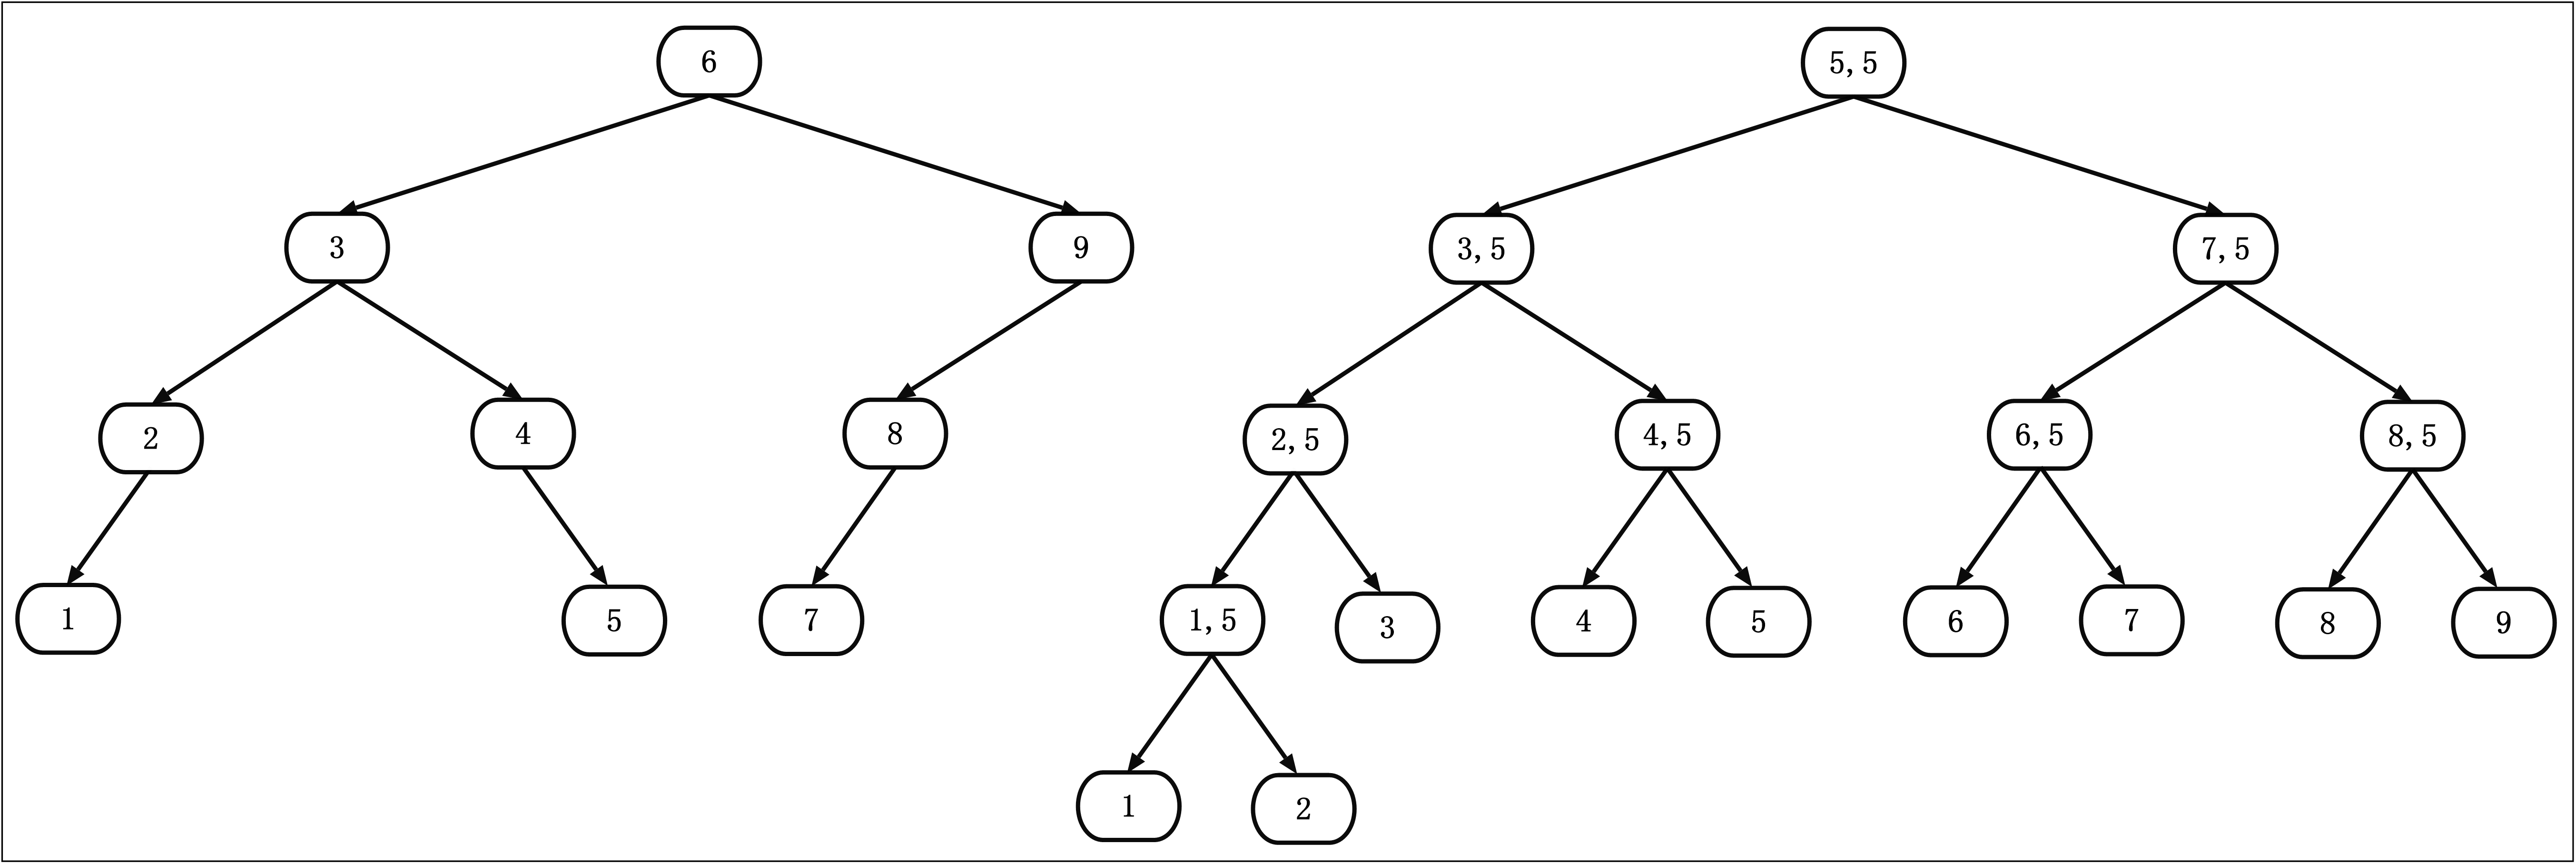
\includegraphics[width=1\textwidth]{Medien/DynOpt/lowerBoundTree}
	\caption{Rechts ist ein möglicher Lower Bound Tree zum linken BST dargestellt.  }
	\label{fig:lowerBoundTree}
\end{figure}

\noindent Nun wird die Funkion $_X(T, Y, X) $ vorgestellt. Ihre Parameter sind ein BST $T$, ein Lower Bound Tree $Y$ und eine Zugriffsfolge $X$. $Y$ und $X$ müssen passend für $T$ erstellt sein, ansonsten ist $_X(T, Y, X) $ undefiniert. Die Auswertung erfolgt zu einer natürlichen Zahl. Sei $U$ die Menge der inneren Knoten von $Y$ und $m$ die Länge von $X$. Sei $u \in U$ und $l$ der kleinste Schlüssel eines Blattes im Teilbaum mit der Wurzel $u$, sowie $r$ der größte Schlüssel eines solchen Blattes. Sei $v$ der gemeinsame Vorfahre der Knoten mit einem Schlüssel aus $\left[l, r\right]$  in $T$, mit der größten Tiefe. Sei $o$ die Folge $o_0, o_1,..,o_m =  \mathit{key}(v) \circ X^r_l$. $i \in \left[1,m\right]$ ist eine  \mbox{\textbf{u-Transition}}, wenn $\left( o_{i-1} < u \land o_i > u \right) \lor \left( o_{i-1} > u \land o_i < u \right)$ gilt. Die Funktion $\mathit{score}\left(u\right) \colon U \rightarrow \mathbb{N}$ ist definiert durch $\mathit{score}\left(u\right) = \vert\{i \in \mathbb{N}\ \vert \textit{i ist eine u-Transition}\} \vert$. Mit Hilfe von $\mathit{score}$ kann nun  $_X(T, Y, X) $ definiert werden:

\begin{align*}
_X(T, Y, X)  = m + \sum_{u \in U} {\mathit{score}} \left(u\right)
\end{align*} 

\noindent Im eigentlichen Satz wird $\mathit{W\left(X, T\right)} \geq {_X(T, Y, X)} $ gezeigt werden. Dafür werden aber noch ein Lemma und einige Begriffe benötigt.\\ Der \textbf{linke innere Pfad} $\left(v_0,v_1,..,v_n \right)$ eines Knotens $v$ ist der längst mögliche Pfad für den gilt: $v_0$ ist das linke Kind von $v$ und für $i \in \{1, 2,..,n\}$, $v_i$ ist das rechte Kind von $v_{i-1}$. Der \textbf{rechte innere Pfad} $\left(v_0,v_1,..,v_n \right)$ eines Knotens $v$ ist der längst mögliche Pfad für den gilt: $v_0$ ist das rechte Kind von $u$ und $v_i$ ist das linke Kind von $v_{i-1}$.\\ $T^r_l$ ist ein mit $\left[l,r\right]$ von $T$ abgeleiteter BST, so dass er genau die Schlüssel aus $T$ enthält, die in $\left[l, r\right]$ liegen. Sei $v_d$ der gemeinsame Vorfahre der Knoten mit einem Schlüssel aus  $\left[l,r\right]$ in $T$, mit der größten Tiefe. (Existiert ein solcher nicht, ist $T^r_l$ der leere Baum). Es muss $\mathit{key}(v_d) \in \left[l,r\right]$ gelten. Denn falls $v_d$ ein Blatt ist, ist sein Schlüssel der Einzige aus $\left[l,r\right]$. Hat $v_d$ genau ein Kind $v_{c}$ und $\mathit{key}(v_d) \notin \left[l,r\right]$, dann wäre $v_{c}$ ein gemeinsamer Vorfahre der entsprechenden Knoten, mit größerer Tiefe. Hat $v_d$ zwei Kinder gibt es drei Fälle:
\begin{itemize}
	\item Im linken und im rechten Teilbaum von $v_d$ sind Schlüssel aus $\left[l,r\right]$ enthalten. Dann muss aufgrund der Links-Rechts-Beziehung  $\mathit{key}(v_d)$ auch in $\left[l,r\right]$ enthalten sein.
	\item In genau einem Teilbaum von $v_d$ sind Schlüssel aus $\left[l,r\right]$ enthalten. Sei $v_{c}$ die Wurzel dieses Teilbaumes. Gilt zusätzlich $\mathit{key}(v_d) \notin \left[l , r\right]$, dann wäre $v_c$ ein  gemeinsamer Vorfahre der entsprechenden Knoten, mit größerer Tiefe.
	\item In den beiden Teilbäumen sind keine Schlüssel aus $\left[l,r\right]$ enthalten.  Dann muss $\mathit{key}(v_d)$ der einzige in $T^r_l$ enthaltene Schlüssel sein.
\end{itemize}

\noindent Ein Knoten $u_d$ mit dem Schlüssel $\mathit{key}(v_d)$ bildet die Wurzel von $T^r_l$. Nun wird beschrieben, wie Knoten zu $T^r_l$ hinzugefügt werden.
Dazu werden zwei Mengen verwendet. $U$ ist eine zu Beginn leere Menge. $W$ enthält zu Beginn $u_d$.
\begin{enumerate}
	\item Gilt $U = W$, beende das Verfahren.
	\item Sei $w \in W$ ein Knoten mit $w \notin U$.  Sei $v$ der Knoten in $T$ mit \mbox{$\mathit{key}(w ) = \mathit{key}(v)$}.  
	\item Existiert das linke Kind von $v$ nicht, weiter mit Punkt $4$. Ansonsten sei  $P_l$ der linke innere Pfad von $v$. Enthält $P_l$ keinen Knoten mit einem Schlüssel $\geq l$, weiter mit Punkt $4$. Ansonsten sei $k_l$ der Schlüssel des Knotens mit der kleinsten Tiefe in $P_l$, für den gilt $k_l \geq l$. Erzeuge einen Knoten $w_l$ mit dem Schlüssel $k_l$ und füge ihn als das linke Kind an $w$ an. Füge $w_l$ zu $W$ hinzu.
	\item Existiert das rechte Kind von $v$ nicht, weiter mit Punkt $5$. Ansonsten sei $P_r$ der rechte innere Pfad von $v$. Enthält $P_r$ keinen Knoten mit einem Schlüssel $\leq r$, weiter mit Punkt $5$. Ansonsten sei $k_r$ der Schlüssel des Knotens mit der kleinsten Tiefe in $P_r$, für den gilt  $k_r \leq r$. Erzeuge einen Knoten $w_r$ mit dem Schlüssel $k_r$ und füge ihn als das rechte Kind an $w$ an. Füge $w_r$ zu $W$ hinzu.	
	\item Füge $w$ zu $U$ hinzu, weiter mit Punkt $1$.
\end{enumerate}
Das Verfahren muss terminieren, da die Anzahl der Knoten von $T$ endlich ist. So konstruiert muss $T^r_l$ ein BST sein. Ein Beispiel stellt Abbildung \ref{fig:T_r_l} dar. 
\begin{figure}[H]
	\centering
	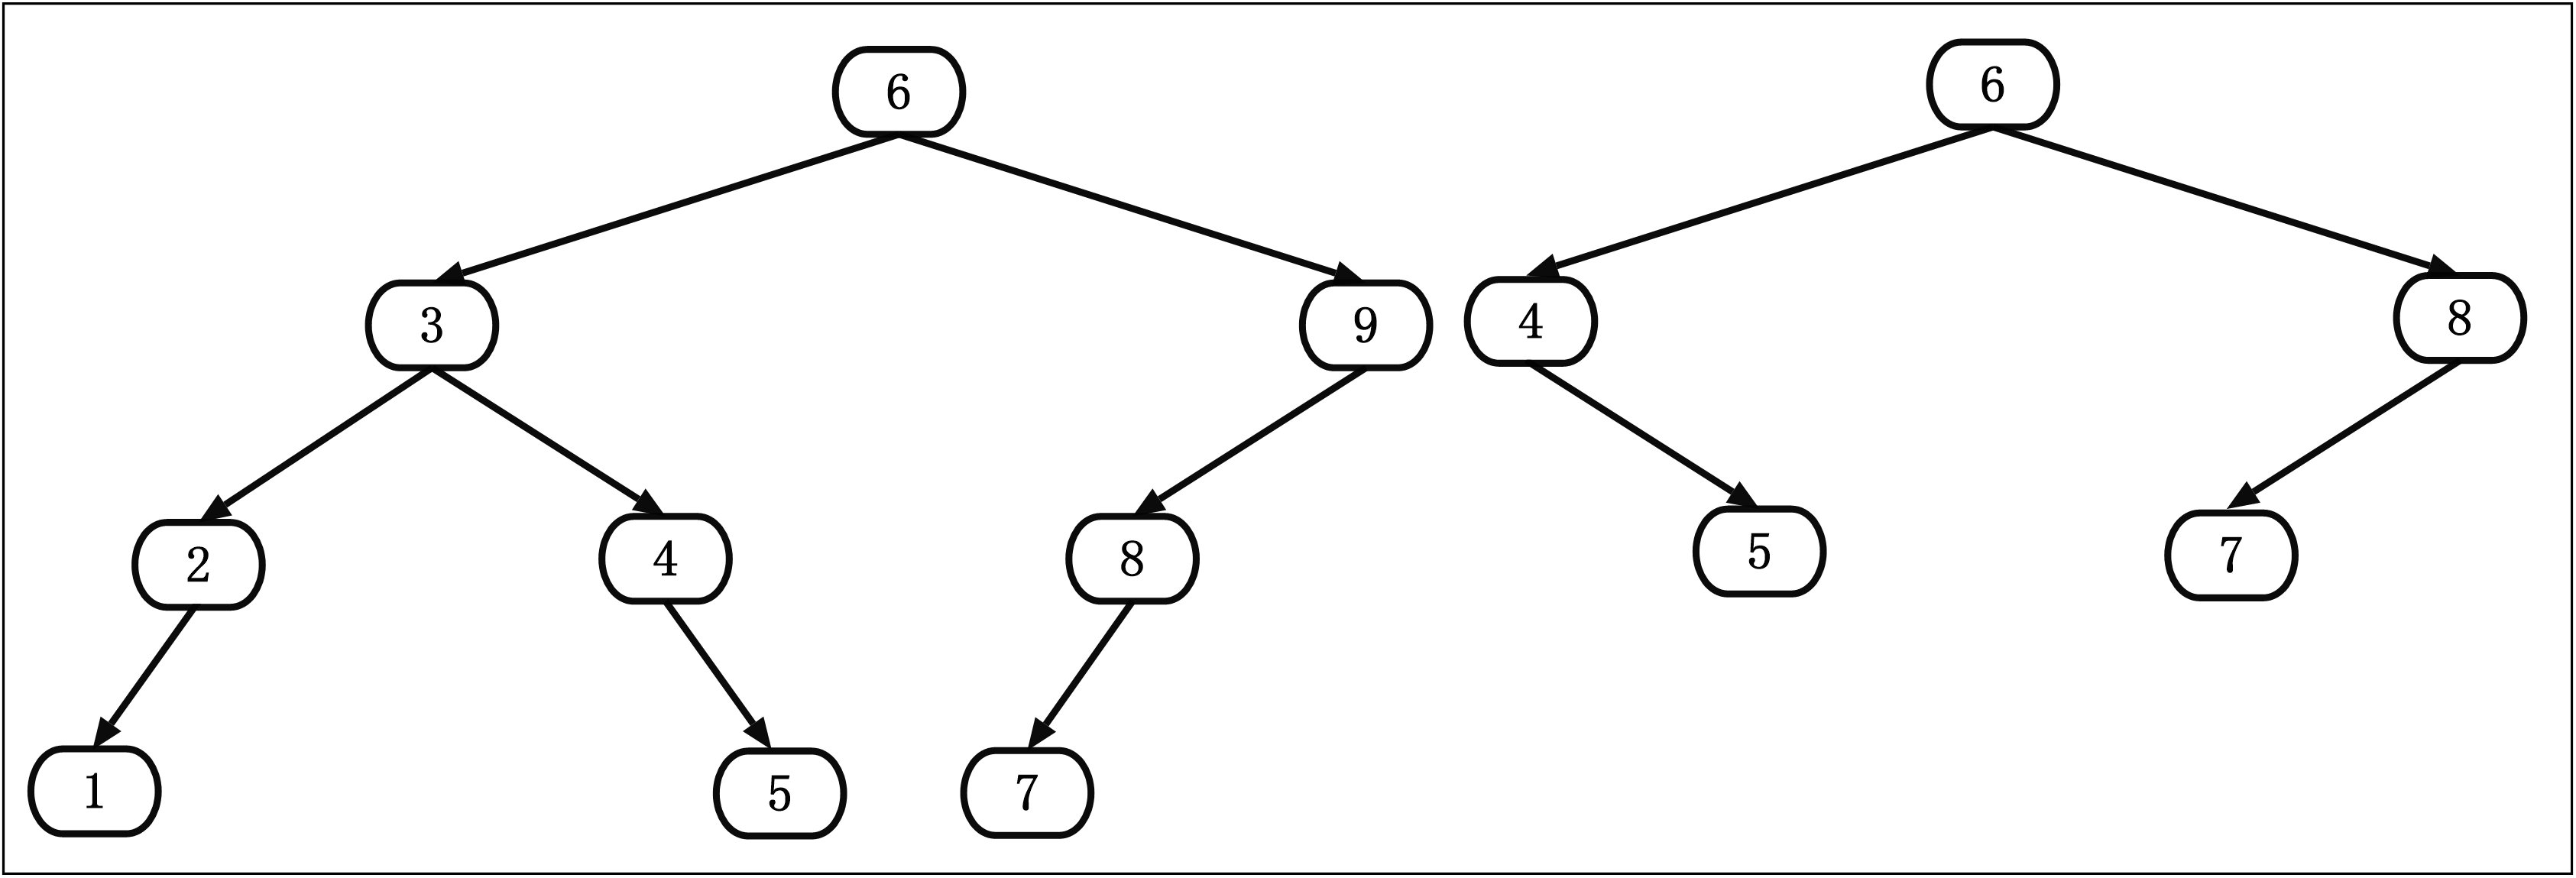
\includegraphics[width= 1\textwidth]{Medien/DynOpt/T_r_l}
	\caption{Links ein BST $T$, rechts ein davon abgeleiteter BST $T^8_4$ .  }
	\label{fig:T_r_l}
\end{figure}

\noindent Sei $K_1$ die Schlüsselmenge von $T$ und $K_2$ die von $T^r_l$. Sei ${K^r_l = K_1 \cap \{i \in \mathbb{N}\vert i \in \left[l,r\right] \}}$. Jetzt wird noch darauf eingegangen, warum $K_2 = K^r_l$ gilt. \\

\noindent $K_2 \subseteq  K^r_l$ ergibt sich direkt aus dem Verfahren zur Konstruktion von $T^r_l$.\\

\noindent $ K^r_l \subseteq K_2$:\\
Sei $k \in K^r_l$ und $v_k$ der Knoten in $T$ mit $\mathit{key}(v_k) = k$. Es muss einen Pfad $P_T = \left(v_0,..,v_n\right)$ in $T$ geben, mit $v_0 = v_d$ und $v_n = v_k$. Sei $m$ die Anzahl der Knoten in $P_T$, mit einem Schlüssel aus  $\left[l,r\right]$. Nun folgt Induktion über $m$.\\
Für $m = 1$ gilt $k = \mathit{key}\left(v_d\right)$  und $k \in K_2$. \\
Induktionsschritt:\\
Sei $w$ der Index des Knotens mit der größten Tiefe in $ v_0,..,v_{n-1}$, mit\\ $\mathit{key}(v_w) \in~K_2$. Nach Induktionsannahme gibt es einen Knoten $u_w$ mit $\mathit{key}(u_w) = \mathit{key}(v_w)$ in $T^r_l$.  Es sei $\mathit{key}(v_w) > \mathit{key}(v_k)$, der andere Fall ist symmetrisch. Ist $v_k$ das linke Kind von $v_w$, dann enthält das linke Kind von $u_w$ den Schlüssel $\mathit{key}(v_k)$. Anderenfalls gilt für alle $v_j$, mit $w < j < k$, $\mathit{key}(v_j) < l \leq \mathit{key}(v_k)$. Somit muss $v_{w+1}$ ein linkes Kind sein und die Knoten in $P_T$ mit größerer Tiefe als der von $v_{w+1}$ müssen rechte Kinder sein. Damit ist auch in diesem Fall ein Knoten $u_k$ mit $\mathit{key}(u_k) = \mathit{key}(v_k)$ das linke Kind von $u_w$.  \\

\noindent Nun kommen wir zum Lemma:\\






\noindent Sei $v$ ein Knoten in $T$. Ein Knoten in $T^r_l$ mit dem Schlüssel $\mathit{key}(v)$ wird dann mit $v^*$ bezeichnet.  

\begin{Lemma}  \label{lemmaWilber1} Es sei $T$ ein BST mit Knoten $u, v$, so dass $u$ ein Kind von $v$ ist. $T'$ ist der BST, der durch Ausführen der Rotation $\left(\mathit{key}\left(u\right),\mathit{key}\left(v\right)\right)$ aus $T$ entsteht. Gilt $\mathit{key}\left(u\right),\mathit{key}\left(v\right) \in \left[l,r\right]$, dann ist ${T'}^r_l$ der BST, der aus $T^r_l$ durch Ausführen von  $\left(\mathit{key}\left(u\right),\mathit{key}\left(v\right)\right)$ entsteht. Anderenfalls gilt ${T'}^r_l = T^r_l$.
\end{Lemma}
\begin{proof}
	\noindent Für $u,v \notin \left[l,r\right]$ wird bei keinem inneren Pfad ein Knoten mit einem Schlüssel aus $\left[l,r\right]$ entfernt oder hinzugefügt.
	Nun werden die vier Fälle betrachtet, bei denen entweder $\mathit{key}\left(u\right)$ oder $\mathit{key}\left(v\right)$ in $\left[l,r\right]$ liegt.
	\begin{enumerate}
		\item $u$ ist das linke Kind von $v$ und $\mathit{key}\left(u\right) < l$:\\
		Sei $w^*$ ein Knoten aus $T^r_l$ und $w'^*$ der aus $T'{^r_l}$, mit $\mathit{key}(w^*) = \mathit{key}(w'^*)$. Es muss gezeigt werden, dass wenn $w^*$ ein linkes, bzw. rechtes Kind mit dem Schlüssel $k$ hat, dann gilt dies auch für $w'^*$. Da \\$\mathit{key}(u) < l \leq \mathit{key}(w) $ gilt, kann weder $u$ noch $v$ im rechten Teilbaum von $w$ enthalten sein. Somit ist bezüglich des rechten Kindes nichts zu zeigen. 
		Sei $P_l$ der linke innere Pfad von $w$ und $ {P_l}'$ der linke innere Pfad von $w'$. Ist $v$ nicht in $P_l$ enthalten und gilt $v \neq w$ dann gilt $P_l = P{_l}'$. Sei $w = v$, dann gilt $P_l = u  \circ  {P_l}'$, vergleiche Abbildung \ref{fig:Rechtsrotation} und da $\mathit{key}(u) < l$, haben die linken Kinder von $w^*$ und $w'^*$ den gleichen Schlüssel. Nun sei $v$ in $P_l$ enthalten. Dann unterscheiden sich  $P_l$ und  ${P_l}'$ dadurch, dass ein Knoten mit $\mathit{key}(u)$ in $P'_l$ enthalten ist. Mit $u < l$ gilt aber, dass sich $w^*$ und $w'^*$ bezüglich des Schlüssels ihres linken Kindes nicht unterscheiden.
	   	\item $u$ ist das rechte Kind von $v$ und $\mathit{key}\left(u\right) > r$:\\
	    Links-rechts-symmetrisch zu Fall 1. 	
		\item $u$ ist das linke Kind von $v$ und $\mathit{key}\left(v\right) > r$:\\
		Durch Vertauschen der Bezeichnungen von $v$ und $u$ entsteht aus $T'$ von Fall 2 durch Ausführung der Rotation auf dieser Konstellation wieder $T$ aus Fall 2. Somit muss nichts weiter gezeigt werden. 
		\item $u$ ist das rechte Kind von $v$ und $\mathit{key}\left(v\right) < l$:\\
		Links-rechts-symmetrisch zu Fall 3. \\
		
	\end{enumerate}	
	\noindent Übrig bleibt noch die Konstellation $\mathit{key}\left(u\right),\mathit{key}(v) \in \left[l,r\right]$. 
	Betrachtet wird eine Rechtsrotation $\left(\mathit{key}\left(u\right),\mathit{key}\left(v\right)\right)$. Die Linksrotation ist wieder symmetrisch. 
	 $T{^r_l}'$ entsteht durch das Ausführen der Rotation  $\left(\mathit{key}\left(u\right),\mathit{key}\left(v\right)\right)$ auf $T{^r_l}$. Zu zeigen ist ${T'}^r_l = T{^r_l}' $.\\
	Es werden zuerst die möglichen Veränderungen an inneren Pfaden von $T$ betrachtet.
	\begin{enumerate}
		\item Sei $u_r$ das rechte Kind von $u$. Sei $\left(u,u_r,v_1, v_2,..,v_n\right)$ der linke innere Pfad von $v$, dann ist $\left({u_r}',{v_1}',{v_2}',..,{v_n}'\right)$ der linke innere Pfad von $v'$. Es gilt ${l \leq \mathit{key}\left(u\right) < \mathit{key}\left(u_r\right) < \mathit{key}\left(v\right) \leq r}$. Damit ist ${{u_r}'}^*$ das linke Kind von ${v'}^*$.
		\item Sei $\left(v_1, v_2,..,v_n\right)$ der rechte innere Pfad von $u$, dann ist $\left(v',{v_1}', {v_2}',..,{v_n}'\right)$ der rechte innere Pfad von $u'$. Damit ist ${v'}^*$ das rechte Kind von ${u'}^*$.
		\item Ist $v$ das linke Kind eines Knotens $z$ mit $\mathit{key}(z) \in \left[r,l\right]$, dann sei  $\left(v,v_1, v_2,..,v_n\right)$ der linke innere Pfad von $z$. Dann ist  $\left(u',v',{v_1}', {v_2}',..,{v_n}'\right)$ der linke innere Pfad von $z'$. Damit ist ${u'}^*$ das linke Kind von ${z'}^*$.\\
		Ist $v$ das rechte Kind eines Knotens $z$ mit $\mathit{key}(z) \in \left[r,l\right]$, dann sei  $v,u, v_1, v_2,..,v_n$ der rechte innere Pfad von $z$. Dann ist  $\left(u',{v_1}', {v_2}',..,{v_n}'\right)$ der rechte innere Pfad von $z'$. Damit ist ${u'}^*$ das rechte Kind von ${z'}^*$.
		\item  Sei nun $v$ das Kind eines Knotens $z$ mit $\mathit{key}(z) \notin \left[r,l\right]$. Sei $a$ ein Knoten mit $\mathit{key}(a) \in \left[r,l\right]$. 
		Als erstes seien $z$ und $v$ im linken inneren Pfad von $a$ enthalten. Dann ist ${{u}'}^*$ das linke Kind von ${a'}^*$.\\
		Nun seien $z$ und $v$ im rechten inneren Pfad von $a$ enthalten. Dann ist ${{u}'}^*$ das rechte Kind von ${a'}^*$.\\
	\end{enumerate}
	\noindent Nun wird auf ${T}^r_l$ die Rotation $ \left(\mathit{key}\left(u^*\right),\mathit{key}\left(v^*\right)\right)$ ausgeführt. ${{u_r}^*}'$ ist das linke Kind von $v{^*}'$. $v{^*}'$ ist das rechte Kind von $u{^*}'$. Ist $v^*$ das linke, bzw. rechte Kind eines Knotens $b^*$, dann ist $u{^*}'$ das linke, bzw. rechte Kind von $b{^*}'$.
	 Damit gilt ${T'}^r_l = T{^r_l}'$.\\
	
\end{proof}


\begin{Satz} \label{satzWilber1} Es sei $T_0$ ein standard BST mit der Schlüsselmenge\\ ${K = \{  i \in \mathbb{N} \vert i \in \left[j,k\right] \textit{ mit } j,k \in  \mathbb{N} \}} $. Sei $Y$ ein für $T_0$ erstellter Lower Bound Tree und $X$ eine zu $T_0$ erstellte Zugriffsfolge mit Länge $m$. Dann gilt\\  $W\left(X, T_0\right) \geq {_X(T_0, Y, X)} $.  
\end{Satz}
\begin{proof}
	Sei $U$ die Menge der inneren Knoten von $Y$. Die Kosten zum Ausführen von $X$ sind die \textit{Anzahl der Einzelschritte} $ +~m$. Es reicht also aus zu zeigen, dass mindestens $\sum_{u \in U} {\mathit{score}} \left(u\right)$ Rotationen benötigt werden. Es wird Induktion über  $n = \vert K \vert$ angewendet. Sei $n = 1$, dann gibt es keinen inneren Knoten in $Y$ und $\sum_{u \in U} {\mathit{score}} \left(u\right) = 0$. Der Induktionsanfang ist somit gemacht. Im Folgenden sei $n \geq 2$.\\
	Sei $R = r_1,r_2,..,r_l$ die Folge der insgesamt durchgeführten Rotationen. Für $i \in \{1,..,l\}$ sei $T_i$ der BST, der entsteht, nachdem $r_i$ auf $T_{i-1}$ ausgeführt wurde. Sei $w$ die Wurzel von $Y$, mit dem Schlüssel $k_w$. Sei $Y^1$, bzw. $Y^2$ der linke, bzw. rechte Teilbaum von $w$. Es ist zu beachten, dass $Y^1$ ein Lower Bound Tree zu $T_{1}^{k_w}$ ist und  $Y^2$ einer zu $T^\infty_{k_w}$. ${T_{i}}_1^{k_w}$ wird im Folgenden als ${T_i}^1$ bezeichnet und ${T_{i}}_{k_w}^{\infty}$ als ${T_i}^2$. Aus $n \geq 2$ folgt, dass $w$ ein innerer Knoten ist. Sei  $R^1 = {r^1}_1,{r^1}_2,..,{r^1}_{l^1} = R^{k_w}_1$ und $R^2 = r^2_1,r^2_2,..,r^2_{l^2} = R^\infty_{k_w}$. Mit $M$ wird die Folge bezeichnet, die entsteht, wenn aus $R$ alle Rotationen entfernt werden, die in $R^1$ oder $R^2$ enthalten sind. Sei $l_M$ die Länge von $M$. Es muss $l = l^1 + l^2 + l_M$ gelten, da keine Rotation sowohl in $R^1$, als auch in $R^2$ enthalten sein kann. $X^1$ entsteht durch das Entfernen aller Schlüssel $k > k_w$ aus $X$ und  $X^2$ entsteht durch das Entfernen aller Schlüssel $k < k_w$ aus $X$. Für $j \in \{1,2\}$ sei $U^j$ die Menge der inneren Knoten von $Y^j$. Sei $T^{j*}_0,T^{j*}_1,..,T^{j*}_{l^j}$ die entstehende Folge, wenn aus $T^{j}_0,T^{j}_1,..,T^{j}_{l}$ die $T^j_i$ entfernt werden, für die $T^j_{i-1} = T^j_i$ gilt.\\ 
	Mit  Lemma \ref{lemmaWilber1} kann für $ t \in \{1,2,.., l^1\}$, $T^{1*}_{t}$ durch Ausführung der Rotation $r^1_t$ auf $T^{1*}_{t-1}$ abgeleitet werden. Für $ t \in \{1,2,.., l^2\}$ gilt analog das Gleiche. Dadurch folgt durch dieses Lemma, falls ein Knoten mit einem Schlüssel $k < w$, bzw. $k > w$ die Wurzel von $T_i$ ist, dann muss die Wurzel von $T^1_i$, bzw. $T^2_i$ auch den Schlüssel $k$ haben. $R^j$ bringt also der Reihe nach die Knoten mit den Schlüsseln aus $X^j$ an die Wurzel von $T^j$ und  $X^j$ kann als Zugriffsfolge für $T^j$ aufgefasst werden. Da die Knotenzahl in $T^j$ kleiner $n$ sein muss, gilt mit der Induktionsannahme  $l^j \geq \sum_{u \in U^j} {\mathit{score}} (u)$.\\
	Sei $\sigma = \mathit{key}(w) \circ X$. Sei $a$ eine $w$-Transition. Nun wird angenommen, dass $\sigma_{a-1} < \mathit{key}(w)  \land \sigma_{a} > \mathit{key}(w)$ gilt. Der andere Fall kann davon problemlos abgeleitet werden. Sei $y$ der Knoten in $T$ mit $\mathit{key}(y) = \sigma_{a-1}$ und $z$ der Knoten in $T$ mit $\mathit{key}(z) = \sigma_{a}$. Nach \textit{access}$(\sigma_{a-1})$ ist $y$ die Wurzel von $T$. $z$ muss sich im rechten Teilbaum von $y$ befinden. Nach  \textit{access}$(\sigma_{a})$ ist $z$ die Wurzel von $T$. $y$ muss sich im linken Teilbaum von $z$ befinden. Somit muss während \textit{access}$(\sigma_{a})$ die Rotation $(\mathit{key}(z),\mathit{key}(y))$ ausgeführt worden sein. $(\mathit{key}(z),\mathit{key}(y))$ muss somit in $M$ enthalten sein. Für jede $w$-Transition ist also mindestens eine Rotation in $M$ enthalten. Also gilt $l_M \geq  \mathit{score} \left(w\right)$.\\
	Zusammengefasst ergibt sich:
	
	\begin{align*}
	l = l^1 + l^2 + l_M \geq \sum_{u \in U^1} {\mathit{score}} (u) + \sum_{u \in U^2}{\mathit{score}} (u) +  {\mathit{score}} (w)
	\end{align*}
	
	
	
	
\end{proof}

\noindent   $_X(T, Y, X)$ ist also eine untere Schranke für die Ausführungszeit von standard BSTs und damit asymptotisch auch für allgemeine BSTs.  


\subsection{Bit Reversal Permutation } \label{abschnittBitReversal}
In diesem Abschnitt wird gezeigt, dass es Zugriffsfolgen mit Länge $m$ gibt, so dass für die Laufzeit beliebiger BST $T$ $\Omega\left(m \log\left( n\right)\right)$ gilt, mit $n$ ist die Anzahl der Knoten von $T$. Hier werden speziell die Zugriffsfolgen betrachtet, die als \textbf{Bit Reversal Permutation} bezeichnet werden. 
Dafür wird die erste untere Schranke von Wilber verwendet und ein Beweis ist ebenfalls in \cite{wilberLowerBounds} enthalten. \\
Nun wird zunächst auf den Aufbau einer solchen Zugriffsfolge eingegangen. Sei $l \in \mathbb{N}$ und $i \in \{0,1,..,l-1\}$. Eine Folge  $b_{l-1},b_{l-2},..,b_0$ mit $b_i \in \{0,1\}$, kann als Zahl zur Basis $2$ interpretiert werden. $T$ enthält alle Schlüssel die als eine solche Folge dargestellt werden können. Die Schlüsselmenge von $T$ ist deshalb $K_l = \{0,1,..,2^l -1\}$. 
Die Funktion $\mathit{br}_l(k)\colon K \rightarrow K$ ist wie folgt definiert. Sei {$b_{l-1},b_{l-2},..,b_{0}$} die Binärdarstellung von $k$, dann gilt:
\begin{align*}
\mathit{br}_l(k) = \sum_{i = 0}^{l-1} b_{\left(l-1-i\right)} \cdot 2^i
\end{align*}
$\mathit{br}_l(k)$ gibt also gerade den Wert der \enquote{umgekehrten} Binärdarstellung von $k$ zurück. Die Bit Reversal Permutation zu $l$ ist die Zugriffsfolge\\ ${\mathit{br}_l(0),\mathit{br}_l(1),..,\mathit{br}_l(2^l-1)}$. Tabelle \ref{tab:bitReversal} zeigt die Bit Reveral Permutation mit $l  = 4$.\\
 Sei $y = \max\left(K_l\right) /2 = 2^{l-1} - 0,5 $. Da $b_0$ in den Binärdarstellungen zu $0, 1,.., 2^l-1$ alterniert, alterniert $b_{l-1}$ in $X$. Aus $2^{l-1} > y$ folgt \\ $\mathit{br}_l(k) < y \Rightarrow \mathit{br}_l(k +1) > y$ und $\mathit{br}_l(k) > y \Rightarrow \mathit{br}_l(k +1) < y$. Da $\vert K_l \vert = 2^l$, sind im vollständig balancierten Lower Bound Tree $Y$ zu $T$ alle Ebenen vollständig mit Knoten besetzt. Sei $w$ die Wurzel von $Y$. Da im linken Teilbaum von $w$ genau so viele Blätter wie im rechten Teilbaum vorhanden sein müssen, kann nur $y$ der Schlüssel von $w$ sein. Zu einer Zugriffsfolge $X = x_0,x_1,..,x_m$ bezeichnet $X^r_l$ wieder die Zugriffsfolge, die entsteht, wenn aus $X$ alle Schlüssel $k$, mit $k < l \lor k > r$ entfernt werden. $X + i$ mit $i \in \mathbb{N}$ bezeichnet im Folgenden die Folge $x_0 + i, x_1 + i,.., x_m + i$.\\

\begin{table}
	\begin{center}
		\begin{tabular}[c]{|l|l|l|l|}
			\hline
			$i$ & $\mathit{bin}\left(i\right)$ &$\mathit{bin}\left(\mathit{br}\left(i\right)\right)$  &$x_i$\\
			\hline
			$0$ & $0000$ &$0000$  &$0$\\
			\hline
			$1$ & $0001$ &$1000$  &$8$\\
			\hline
			$2$ & $0010$ &$0100$  &$4$\\
			\hline
			$3$ & $0011$ &$1100$  &$12$\\
			\hline
			$4$ & $0100$ &$0010$  &$2$\\
			\hline
			$5$ & $0101$ &$1010$  &$10$\\
			\hline
			$6$ & $0110$ &$0110$  &$6$\\
			\hline
			$7$ & $0111$ &$1110$  &$14$\\
			\hline
			$8$ & $1000$ &$0001$  &$1$\\
			\hline
			$9$ & $1001$ &$1001$  &$9$\\
			\hline
			$10$& $1010$ &$0101$  &$5$\\
			\hline
			$11$& $1011$ &$1101$  &$13$\\
			\hline
			$12$ &$1100$ &$0011$  &$3$\\
			\hline
			$13$ &$1101$ &$1011$  &$11$\\
			\hline
			$14$ &$1110$ &$0111$  &$7$\\
			\hline
			$15$ &$1111$ &$1111$  &$15$\\
			\hline
		\end{tabular}
		\caption{Die Bit Reversal Permutation für $l=4$} 
		\label{tab:bitReversal}
	\end{center}
\end{table}



\newtheorem{Korollar1}{Korollar}[section]
\begin{Korollar1} Sei $l \in \mathbb{N}$. Sei $T$ ein BST mit der Schlüsselmenge\\ ${K_l = \{0,1,..,2^l -1\}}$ und $n = 2^l$. Sei $X = x_0, x_1,..,x_{n-1}$ die Bit Reversal Permutation zu $l$ und $Y$ der vollständig balancierte Lower Bound Tree zu $T$. Dann gilt  $W\left(X,T\right) \geq n \log_2 \left(n\right) + 1 $. 
\end{Korollar1}
\begin{proof}
	Sei $U$ die Menge der inneren Knoten von $Y$. Mit Satz \ref{satzWilber1} reicht es aus, 
	
	\begin{align*}
	\sum_{u \in U} {\mathit{score}\left(u\right)} \geq n \log_2\left( n\right) + 1 - n 
	\end{align*} 
	zu zeigen. Dies geschieht mit Induktion über $l$. Für $l = 0$ besteht $Y$ aus einem einzigen Blatt. Damit gilt:\\ $ \sum_{u \in U} {\mathit{score}\left(u\right)} = 0 = n \log_2 \left(n\right) + 1 - n $. \\
	Nun sei $l > 0$. Sei $w$ die Wurzel von $Y$, mit $k_w = \mathit{key}(w)$. Sei $T_0^{k_w}$ ein BST mit der Schlüsselmenge $K_0^{k_w} =\{k \in \mathbb{N}\vert k \leq k_w\} = \{k \in \mathbb{N}\vert k \leq 2^{l-1} - 1\}$ und $T_{k_w}^\infty$ ein BST mit der Schlüsselmenge \mbox{$ K^\infty_{k_w} = \{k \in \mathbb{N}\vert \exists n \in K_0^{k_w}\colon  k = n + 2^{l-1}\}$}. Sei $Y^1$, bzw. $Y^2$ der linke, bzw. rechte Teilbaum von $w$ und $U^1$, bzw. $U^2$ die Menge der inneren Knoten von $Y^1$, bzw. $Y^2$. $Y^1$ und $Y^2$ sind vollständig balancierte Lower Bound Trees zu $T_0^{k_w}$ und $T_{k_w}^\infty$. $X^{k_w}_0$ ist die Bit Reversal Permutation für $T_0^{k_w}$. Außerdem gilt $X_{k_w}^\infty = X^{k_w}_0 + 2^{l-1}$. Mit der Induktionsannahme gilt deshalb für $i \in \{1,2\}$:
	\begin{align*}
	\sum_{u \in U^i} {\mathit{score}\left(u\right)} \geq  \frac{n}{2} \log_2 \left(\frac{n}{2} \right) + 1 - \frac{n}{2}  
	\end{align*}
	Sei $j \in \{1, 2,.., n-1\}$. Aus $\left(x_j < k_w \Rightarrow x_{j-1} > k_w \right) \land \left(x_j > k_w \Rightarrow x_{j-1} < k_w \right)$ folgt $\mathit{score}\left(w\right) \geq n-1$. \\
	Zusammenfassen ergibt:
	\begin{align*}
	\sum_{u \in U} {\mathit{score}\left(u\right)} &\geq 2 \left( \frac{n}{2}  \log_2 \left(\frac{n}{2} \right) + 1 - \frac{n}{2} \right) + n - 1\\	
	&= n (l-1)  + 1 \\	
	&= n l + 1 -n \\
	&= n \log_2\left( n\right) + 1 - n\\	
	\end{align*}
	
\end{proof}

\noindent Die Schlüsselmenge  wurde beim Korollar auf ${K_l = \{0,1,..,2^l -1\}}$ festgelegt. Vielleicht wäre es aber mit einer anderen Schlüsselmenge $K$ möglich $X$ schneller auszuführen? In jedem Fall müsste $K_l \subseteq K$ gelten. Sei $R$ die Folge von Rotationen, die beim Ausführen von $X$ bei einem BST $T$ mit der Schlüsselmenge $K$ entsteht. Sei $y = 2^l -1$. Mit Lemma \ref{lemmaWilber1} ist dann $R_0^y$ eine Folge von Rotationen zum Ausführen von $X$ auf $T_0^y$ und die Länge von $R$ kann nicht kleiner als die von $R_0^y$ sein. 



\subsection{Amortisierte Laufzeitanalyse}
Im nächsten Abschnitt werden die Kosten von amortisierten Laufzeitanalysen verwendet. Deshalb wird diese hier nun vorgestellt.
Sei $i \in \{0,..,m\}$. Bei der \textbf{amortisierten Laufzeitanalyse} wird eine Folge von $m$ Operationen betrachtet. Hierbei kann es sich $m$ mal um die gleiche Operation handeln oder auch um verschiedene. Die \textbf{tatsächlichen Kosten}  $t_i$ stehen für die exakt bestimmten Kosten zum Ausführen der $i$-ten Operation. Durch addieren der tatsächlichen Kosten jeder einzelnen Operation ergeben sich die \textbf{tatsächlichen Gesamtkosten}. Stehen für die Laufzeit der Operationen jeweils nur obere Schranken zur Verfügung, kann mit diesen genau so vorgegangen werden, um eine obere Schranke für die Gesamtlaufzeit zu erhalten. So erzeugte obere Schranken können jedoch unnötig hoch sein. Die Idee bei einer amortisierten Analyse ist es, eingesparte Zeit durch schnell ausgeführte Operationen, den langsameren Operationen zur Verfügung zu stellen. Dabei wird insbesondere der aktuelle Zustand der zugrunde liegenden Datenstruktur vor und nach einer Operation betrachtet. Es gibt drei Methoden zur amortisierten Analyse. Bei BSTs wird in der Regel die \textbf{Potentialfunktionmethode} verwendet.
\paragraph{Potentialfunktionmethode:} \label{potentialfunktionsmethode} Eine Potentialfunktion $\Phi(D)$ ordnet einem Zustand einer Datenstruktur $D$ eine natürliche Zahl, \textbf{Potential} genannt, zu. Es bezeichnet $\Phi(D_i)$ das Potential von $D$ nach Ausführung der $i$-ten Operation. Die \textbf{amortisierten Kosten} $a_i$ einer Operation berücksichtigen die von der Operation verursachte Veränderung am Potential, \mbox{$a_i = t_i + \Phi(D_{i}) - \Phi(D_{i-1})$}. Um die \textbf{amortisierten Gesamtkosten} $A$ zu berechnen, wird die Summe der amortisierten Kosten aller Operationen gebildet. 
\begin{align*}
A = \sum_{i = 1}^{m} a_i =  \sum_{i = 1}^{m} \left(t_i + \Phi\left(D_{i}\right) - \Phi\left(D_{i-1}\right)\right) = \Phi\left(D_{m}\right) - \Phi\left(D_{0}\right) + \sum_{i = 1}^{m} t_i 
\end{align*}
Folgendes gilt für die Summe der $t_i$:
\begin{align*}
&\sum_{i = 1}^{m} t_i =  \sum_{i = 1}^{m} \left(a_i - \Phi\left(D_{i}\right) + \Phi\left(D_{i-1}\right)\right) = \Phi\left(D_{0}\right) - \Phi\left(D_{m}\right) + \sum_{i = 1}^{m} a_i \\
\Rightarrow &\left( \Phi\left(D_{m}\right) \geq \Phi\left(D_{0}\right) \Rightarrow \sum_{i = 1}^{m} a_i \geq \sum_{i = 1}^{m} t_i \right)
\end{align*}
Ist das Potenzial nach der Ausführung der Operationsfolge also nicht kleiner als zu Beginn, dann sind die amortisierten Gesamtkosten eine obere Schranke für die tatsächlichen Gesamtkosten. Die wesentliche Aufgabe ist es nun eine Potentialfunktion zu finden, bei der die amortisierten Gesamtkosten möglichst niedrig sind und für die $\Phi\left(D_{m}\right) \geq \Phi\left(D_{0}\right)$ gilt. Dies wird jetzt noch an einem einfachen Beispiel demonstriert.

\paragraph{Potentialfunktionmethode am Beispiel eines Stack:} 
Der Stack verfügt wie gewöhnlich über eine Operation \textit{push} zum Ablegen eines Elementes auf dem Stack und über \textit{pop} zum Entfernen des oben liegenden Elements. Zusätzlich gibt es eine Operation \textit{popAll}, die so oft \textit{pop} aufruft, bis der Stack leer ist. Sei $n$ die Anzahl der Elemente die maximal im Stack enthalten sein können. \textit{push} und \textit{pop} können in konstanter Zeit durchgeführt werden und wir berechnen jeweils eine Kosteneinheit. Für die Laufzeit von \textit{popAll} gilt $O(n)$, da \textit{pop} bis zu $n$ mal aufgerufen wird. Für die Gesamtlaufzeit einer Folge von $m$ Operationen kann $O(mn)$ angegeben werden. Mit einer amortisierten Analyse wird nun aber $O(m)$ für einen zu Beginn leeren Stack gezeigt. Als $\Phi$ verwenden wir eine Funktion, welche die aktuelle Anzahl der im Stack enthaltenen Elemente zurück gibt. \textit{push} erhöht das Potential um eins, während \textit{pop} es um eins vermindert. Nun werden die amortisierten Kosten bestimmt: 

\begin{align*}   
&a_{\mathit{push}} = t_{\mathit{push}} + \Phi_{i} - \Phi_{i-1}  &= 2\\
&a_{\mathit{pop}} = t_{\mathit{pop}} + \Phi_{i} - \Phi_{i-1}  &= 0\\
&a_{\mathit{popAll}} = n \cdot a_{\mathit{pop}} &= 0
\end{align*}\\
Alle drei Operationen haben konstante amortisierte Kosten. Auf jeden Fall gilt $ \Phi_m \geq  \Phi_0 = 0 $. Für die Ausführungszeit der Folge gilt deshalb $O(m)$. Das Potential kann aufgrund einer Folge von Operationen um maximal $n$ verringert werden. Deshalb kann $O\left(m + n\right)$ verwendet werden, wenn der Stack zu Beginn nicht leer ist.  \\



\subsection{Eigenschaften eines dynamisch optimalen BSTs. }\label{upperBounds}
Hier werden einige obere Laufzeitschranken für Zugriffsfolgen vorgestellt. Es ist bekannt, dass es obere Schranken sind, da mit dem Splay Baum ein BST bekannt ist, der jede der Schranken einhält. Der Splay Baum wird später noch vorgestellt. Es wird wieder ohne Verlust der Allgemeinheit eine Schlüsselmenge $K = \{1,2,..,n\}$ angenommen. Wenn nicht anders angegeben wird  $X = x_1,x_2,..,x_m$ als Zugriffsfolge verwendet. 


\paragraph{Balanced Property:}
Ein BST erfüllt die Balanced Property, wenn er $X$ in amortisiert $O\left(m + \left(m + n\right) \log \left( n\right)  \right)$ Zeit ausführt. 

\paragraph{Static Finger Property:}
Die Idee hinter dieser Eigenschaft ist, dass es einfacher ist, Zugriffsfolgen schnell auszuführen, wenn ihre Schlüssel betragsmäßig nahe beieinander liegen. Ein BST erfüllt die Static Finger Property, wenn zu jedem Schlüssel $k_f \in K$ für die amortisierte Laufzeit von $X$ 
\begin{align*}
O\left( n \log\left( n\right) +m + \sum_{i = 1}^{m} \log \left( \vert k_f - x_i  \vert	+ 1	\right)\right)
\end{align*}
gilt. 


\paragraph{Statisch optimal:}
Sei $k \in K$ und $q(k)$ die Anzahl des Vorkommens von $k$ in  $X$. Ein BST ist statisch optimal, wenn er Zugriffsfolgen, in denen jeder seiner Schlüssel zumindest einmal enthalten ist, in amortisiert 
\begin{align*}
O\left(m +\sum_{k = 1}^{n}q(k)\log \left( \frac{m}{q(k)} \right)\right) 
\end{align*}
Zeit ausführt. Der Name kommt daher, dass es sich hierbei um eine untere Schranke für die Ausführungszeit von X bei statischen BST handelt \cite{staticOptimal}. Solche ändern ihre Struktur während \textit{access} nicht.

\paragraph{Working Set Property:}
Ein BST mit der Working Set Property führt Zugriffsfolgen schnell aus, bei denen auf die gleichen Schlüssel in kurzen Abständen zugegriffen wird.
Für $x_i$ sei $J_i = \{j \in \mathbb{N} \vert j < i \land x_j = x_i \}$.
Sei $t_{xi} = \max \left(J_i\right)$, falls $J_i$ nicht leer ist, ansonsten $t_{xi} = 0$. $t_{xi}$ liefert also den Index des vorherigen Zugriffes auf $x_i$, falls ein solcher existiert. Sei ${a_i = \vert\{x_j \vert t_{xi} < j \leq i   \} \vert }$.
Ein BST erfüllt die Working Set Property, wenn für seine amortisierte Laufzeit für $X$
\begin{align*}
O\left(n \log\left( n\right) + m +\sum_{i = 1}^{m} \log \left(a_i\right) \right)
\end{align*} 
gilt. 


\paragraph{Dynamic Finger Property:}
Diese Eigenschaft ist der Static Finger Property sehr ähnlich.
Ein BST erfüllt die Dynamic Finger Property, wenn für seine amortisierte Laufzeit für $X$
\begin{align*}
O\left( m + n + \sum_{i = 2}^{m} \log \left(\vert x_{i-1} - x_i  \vert	+ 1	\right)\right)
\end{align*} 
gilt. 

\noindent Abbildung \ref{fig:upperBounds} zeigt Implikationen zwischen den Eigenschaften und basiert auf einer Abbildung aus \cite{upperBounds}.

\begin{figure}[H]
	\centering
	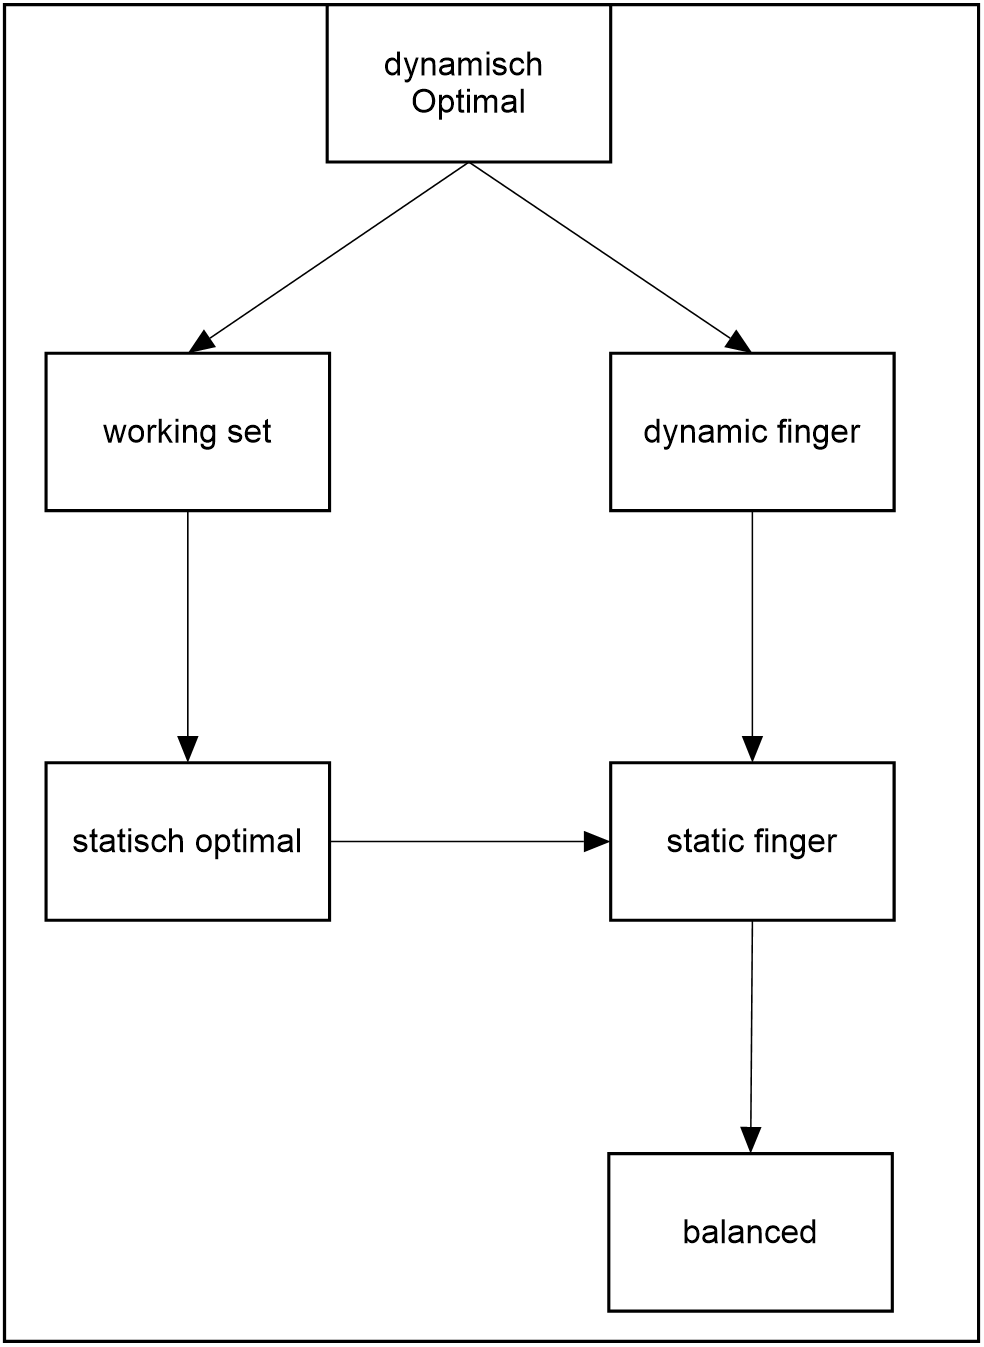
\includegraphics[width= 0.6\textwidth]{Medien/DynOpt/upperBounds}
	\caption{Implikationen zwischen den Eigenschaften, abgeleitet aus einer Abbildung aus \cite{upperBounds}. }
	\label{fig:upperBounds}
\end{figure}


\section{Tango Baum} \label{TangoAbschnitt}
Der Tango Baum ist ein aus BSTs, den \textbf{Hilfsbäumen}, bestehender BST. Auf die Anforderungen an die Hilfsbäume wird in Abschnitt \ref{aufbauDesTango} eingegangen. Der Tango Baum wurde  von Demaine, Harmon, Iacono und Patrascu beschrieben \cite{demainDinamicOpti}, inklusive eines Beweises über seine $\log\left(\log\left(n\right)\right)$-competitiveness. Ebenfalls in \cite{demainDinamicOpti} enthalten ist eine als \textbf{Interleave Lower Bound} bezeichnete Variation der ersten unteren Schranke von Wilber. Da diese für das Verständnis des Tango Baumes wesentlich ist, wird mit ihr gestartet, bevor es zur Beschreibung der Struktur selbst kommt. 


\subsection{Die Interleave Lower Bound} \label{interBound}
Sei $X = x_1,x_2,.,x_m$ eine Zugriffsfolge und sei $K = \{k \in \mathbb{N} \vert k \textit{ ist in $X$ enthalten}\}$. Auch hier wird ein Lower Bound Tree verwendet. Dieser ist jedoch etwas anders definiert als in \mbox{Abschnitt \ref{wilberBound}}. Hier ist der Lower Bound Tree $Y$ zu einer Zugriffsfolge $X$ der komplette BST mit der Schlüsselmenge $K$. Anders als in Abschnitt \ref{wilberBound}  gibt es hier somit zu jeder Zugriffsfolge nur genau einen Lower Bound Tree. Abbildung \ref{fig:demlowerBoundTree} zeigt den Lower Bound Tree zur Zugriffsfolge $1, 2,.., 15$. Zu jedem Knoten $v$ in $Y$ werden zwei Mengen definiert. Die \textbf{linke Region} von $v$ enthält den Schlüssel von $v$, sowie die im linken Teilbaum von $v$ enthaltenen Schlüssel.  Die \textbf{rechte Region} von $v$ enthält die im rechten Teilbaum von $v$ enthaltenen Schlüssel. Sei $l$ der kleinste Schlüssel im Teilbaum mit der Wurzel $v$ und $r$ der größte. Sei  $X^r_l = {x_{1'},x_{2'},..,x_{m'}}$ wie in Abschnitt \ref{wilberBound} definiert. $i \in \{2,3,..,m'\}$ ist ein \textbf{Interleave} durch $v$, wenn $x_{\left(i -1\right)}$ in der linken Region von $v$ liegt und $x_i$ in der rechten Region von $v$ oder umgekehrt. In $Y$ sind Knoten enthalten, bei denen die rechte Region leer ist. Durch diese kann es keinen Interleave geben. Sei $U$ die Menge der Knoten von $Y$ mit einer nicht leeren rechten Region. Sei \textit{inScore($u$)} die Funktion, die zu dem Knoten $u \in U$ die Anzahl der Interleaves durch $u$ zurückgibt.  Die Funktion \textit{IB}$\left(X\right)$ ist definiert durch:
\begin{align*}
\mathit{IB}\left(X\right) = \sum_{u \in U} \mathit{inScore}\left(u\right)
\end{align*}
Sei $T_0$ der BST mit der Schlüsselmenge $K$ auf der $X$ ausgeführt wird. Für $i \in \{1,2,..,m\}$ sei $T_i$ der BST, der entsteht nachdem \textit{access}$\left(x_i\right)$ auf $T_{i-1}$ ausgeführt wurde. Zu $u \in U$ und  $j \in \{0,1,..,m\}$ gibt es einen \textbf{transition point} $v$ in $T_j$. $v$ ist ein Knoten mit folgenden Eigenschaften:\\
\begin{enumerate}
	\item Der Pfad von der Wurzel von $T_j$ zu $v$ enthält einen Knoten, dessen Schlüssel in der linken Region von $u$ enthalten ist.
	\item Der Pfad von der Wurzel von $T_j$ zu $v$ enthält einen Knoten, dessen Schlüssel in der rechten Region von $u$ enthalten ist.
	\item In $T_j$ ist kein Knoten mit den Eigenschaften 1 und 2 enthalten, der eine kleinere Tiefe als $v$ hat. 
\end{enumerate}
\begin{figure}[H]
	\centering
	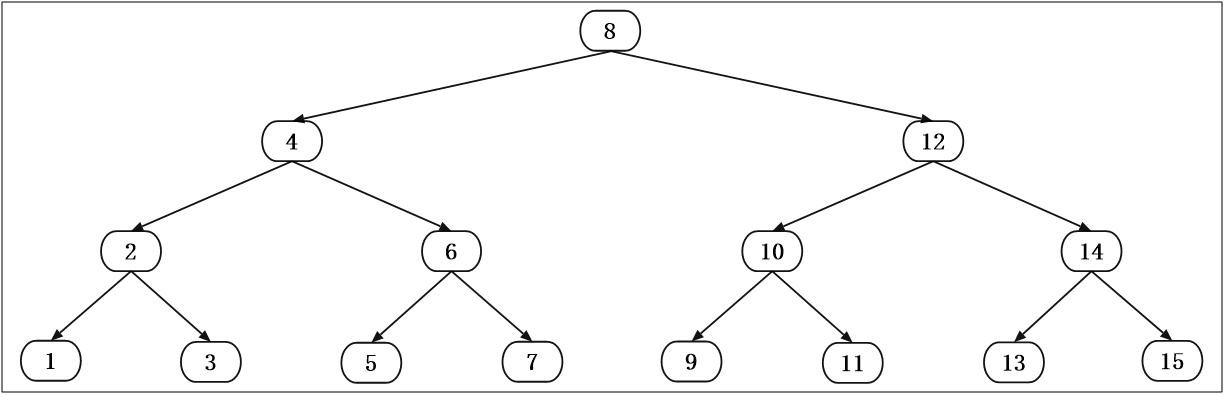
\includegraphics[width=1\textwidth]{Medien/Tango/lowerBoundTree}
	\caption{Der Lower Bound Tree zur Zugriffsfolge $1 ,2, .., 15$.  }
	\label{fig:demlowerBoundTree}
\end{figure}

\noindent Im Beweis dieses Abschnitts wird gezeigt, dass $\mathit{OPT}\left(X\right) \geq \frac{\mathit{IB}\left(X\right)}{2} - n$ gilt, wobei $n$ die Anzahl der Knoten im Lower Bound Tree ist. Dafür werden jedoch noch drei Lemmata zu den Eigenschaften von $Y$ benötigt.\\
 Bei allen dreien wird $X = x_1, x_2,.., x_m$ die Zugriffsfolge sein, die auf einem BST $T_0$ ausgeführt wird. $Y$ ist ein zu $X$ erstellter Lower Bound Tree mit der Schlüsselmenge $K$.
Für $i \in \{1,2,..,m\}$ ist $T_i$ der BST der durch Ausführen von \textit{access}$\left(x_i\right)$ auf $T_{\left(i-1\right)}$ entsteht. Und $U$ ist die Menge der Knoten von $Y$, bei denen die rechte Region nicht leer ist. Außerdem gilt   $j \in \{0,1,..,m\}$.
\begin{Lemma} \label{demaineLemma1}
Es gibt zu jedem Knoten $u \in U$ genau einen transition point in $T_j$. 	
\end{Lemma}


\begin{proof}
	Sei $l$ der kleinste Schlüssel in der linken Region von $u$ und $r$ der größte Schlüssel in der rechten Region. Im Teilbaum mit der Wurzel $u$ sind genau die Schlüssel $K^r_l = \{k \in K \vert k \in \left[l,r\right]\}$ enthalten. Sei $v_l$ der gemeinsame Vorfahre aller Knoten mit einem Schlüssel aus der linken Region von $u$ in $T_j$ mit der größten Tiefe. Sei $v_r$ der gemeinsame Vorfahre aller Knoten mit einem Schlüssel aus der rechten Region von $u$ in $T_j$ mit der größten Tiefe. $\mathit{key\left(l\right)}$, bzw. $\mathit{key\left(r\right)}$ muss selbst in der linken, bzw. rechten Region von $u$ enthalten sein, vergleiche das Bilden von $T^r_l$ in Abschnitt \ref{wilberLowerBoundTree}. Sei $w$ der gemeinsame Vorfahre aller Schlüssel aus der linken und der rechten Region von $u$ in $T_j$ mit der größten Tiefe. Es muss $\mathit{key}\left(w\right) \in \left[l,r\right]$ gelten. Somit muss  $\mathit{key}\left(w\right)$ entweder in der linken oder rechten Region von $u$ enthalten sein. Da $w$ der Knoten mit der kleinsten Tiefe sein muss, für den  $\mathit{key\left(w\right)} \in \left[l,r\right]$  gilt, muss entweder $w = v_l$ oder $w = v_r$ gelten, je nachdem wessen Tiefe kleiner ist. Für den Fall $w = v_l$ ist $v_r$ der transition point in $T_j$ zu $u$ und für den Fall $w = v_r$ ist es $v_l$.
	Es wird der Fall $w = v_l$ betrachtet, der andere kann direkt daraus abgeleitet werden. Im Pfad $P_u = v_0,v_1,..,v_r$ von der Wurzel $v_0$ zu $v_r$ ist $v_l$ enthalten und da $v_r$ ein gemeinsamer Vorfahre der Schlüssel aus der rechten Region von $u$ ist, muss $v_r$ der einzige Knoten mit einem Schlüssel aus der rechten Region von $u$ in $P_u$ sein. Jeder Pfad $P$ in $T_j$ von der Wurzel zu einem Knoten mit einem Schlüssel aus der rechten Region von $u$ muss mit $v_0,v_1,..,v_r$ beginnen. Somit kann es keinen weiteren transition point für $u$ in $T_j$ geben. 
	
\end{proof}
\noindent Der Knoten auf den der Zeiger $p$ zum Ausführen von \textit{access} gerade zeigt wird als \textbf{berührter Knoten} bezeichnet.
Im zweiten Lemma geht es darum, dass sich der transition point $v$ eines Knotens nicht verändern kann, solange $v$ nicht wenigstens einmal der berührte Knoten war.



\begin{Lemma} \label{demaineLemma2} \label{lemmaDemaine2}
 Sei $v$ der transition point in $T_j$ zu einem Knoten $u \in U$.  Sei  \mbox{$l \in \mathit{N}$}, mit \mbox{$j < l \leq m$}. Gilt für alle $x_i$ mit $i \in \left[j + 1,l\right]$: Während der Ausführungszeit von \textit{access}$\left(x_i\right)$ war  $v$  nicht wenigstens einmal der berührte Knoten, dann ist $v$ während der gesamten Ausführungszeit von\\ $\textit{access}\left(x_j\right),\textit{access}\left(x_{j+1}\right),..,\textit{access}\left(x_l\right)$ der transition point zu $u$. 
\end{Lemma}

\begin{proof}
	Sei $v_l$ der gemeinsame Vorfahre aller Knoten mit einem Schlüssel aus der linken Region von $u$ in $T_j$ mit der größten Tiefe. Sei $v_r$ der gemeinsame Vorfahre aller Knoten mit einem Schlüssel aus der rechten Region von $u$ in $T_j$ mit der größten Tiefe. Hier wird wieder ohne Verlust der Allgemeinheit der Fall $v = v_r$ betrachtet. Da $v_r$ nicht berührt wird, wird auch kein Knoten mit einem Schlüssel aus der rechten Region von $u$ berührt. $v_r$ ist somit während der gesamten Ausführungszeit von $\textit{access}\left(x_j\right),\textit{access}\left(x_{j+1}\right),..,\textit{access}\left(x_l\right)$  der gemeinsame Vorfahre der Schlüssel aus der rechten Region von $u$, mit der größten Tiefe. Knoten mit einem Schlüssel aus der linken Region von $u$ könnten berührt werden. Zu einem Ausführungszeitpunkt $t$ kann deshalb ein Knoten $v_{lt} \ne v_l$ der gemeinsame Vorfahre der Knoten mit einem Schlüssel aus der linken Region von $u$ mit der größten Tiefe sein. Da $v_r$ nicht berührt wird kann zu keinem Zeitpunkt $v_l$ im Teilbaum mit der Wurzel $v_r$ enthalten sein. Somit kann auch $v_{lt}$ nicht in diesem Teilbaum enthalten sein. Somit muss die Tiefe von  $v_{lt}$ kleiner sein, als die von $v_r$ und $v_r$ bleibt der transition point von $u$. 
\end{proof}

\noindent Im dritten Lemma wird gezeigt, dass ein Knoten $v$ in $T_j$ nur der transition point zu einem Knoten aus $U$ sein kann.


\begin{Lemma}\label{lemmaDemaine3}
	Sei $u_1, u_2 \in U$, mit $u_1 \ne u_2$.  Sei $v_1$ der transition point zu $u_1$ und $v_2$ der zu $u_2$ in $T_j$. Dann muss $v_1 \neq v_2$ gelten.
\end{Lemma}

\begin{proof}
	Sei $v_l$, bzw. $v_r$ der gemeinsame Vorfahre aller Knoten mit einem Schlüssel aus der linken, bzw. rechten Region von $u_1$ in $T_j$, mit der größten Tiefe.  Sei $w_l$, bzw. $w_r$ der gemeinsame Vorfahre aller Knoten mit einem Schlüssel aus der linken, bzw. rechten Region von $u_2$ in $T_j$ mit der größten Tiefe. Ist weder $u_1$ ein Vorfahre von $u_2$, noch $u_2$ einer von $u_1$, dann muss auch $w_l \ne v_l \land w_l \ne v_r$, sowie $w_r \ne v_l \land w_r \ne v_r$ gelten, da die Teilbäume mit der Wurzel $u_1$ und $u_2$ dann über disjunkte Schlüsselmengen verfügen. Somit müssen die transition points von $u_1$ und $u_2$ unterschiedlich sein. Sei $u_1$ ein Vorfahre von $u_2$. Es werden drei Fälle unterschieden:
	\begin{enumerate}
		\item Ist $\mathit{key}\left(v_1\right)$ nicht im Teilbaum mit der Wurzel $u_2$ enthalten, so kann $v_1$ nicht der transition point von $u_2$ sein.
		\item $\mathit{key}\left(v_1\right)$ ist im Teilbaum mit der Wurzel $u_2$ enthalten und $\mathit{key}\left(v_1\right)$ ist  in der linken Region von $u_1$ enthalten:\\
		Da $u_1$ ein Vorfahre von $u_2$ ist und  $\mathit{key}\left(v_1\right)$ im Teilbaum mit der Wurzel $u_2$ enthalten ist, müssen alle Schlüssel im Teilbaum mit der Wurzel $u_2$ in der linken Region von $u_1$ enthalten sein. Da der Schlüssel von $v_1$ in der linken Region von $u_1$ liegt, muss $v_r$ ein Vorfahre von $v_l$ in $T_j$ sein. $\mathit{key}\left(v_1\right)$ muss somit der Schlüssel von $w_l$, bzw. $w_r$ sein, je nachdem wessen Tiefe kleiner ist. Denn andererseits könnte ein Pfad von der Wurzel von $T_j$ zu $v_1$ angegeben werden, der zwei Knoten aus der linken Region von $u_1$ enthält. Das ist jedoch ein Widerspruch dazu, dass  $\mathit{key}\left(v_1\right)$ in der linken Region von $u_1$ enthalten ist und $v_1$ zudem der transition point für $u_1$ ist.\\
		$v_2$ ist entweder der Knoten $w_l$ oder $w_r$, je nachdem wessen Tiefe größer ist. Somit gilt $v_1 \ne v_2$.
		\item $\mathit{key}\left(v_1\right)$ ist im Teilbaum mit der Wurzel $u_2$ enthalten und $\mathit{key}\left(v_1\right)$ ist in der rechten Region von $u_1$ enthalten:\\
		Symmetrisch zu Fall 2.
	\end{enumerate}
	
	
	
	
	
	
\end{proof}

\begin{figure}[H]
	\centering
	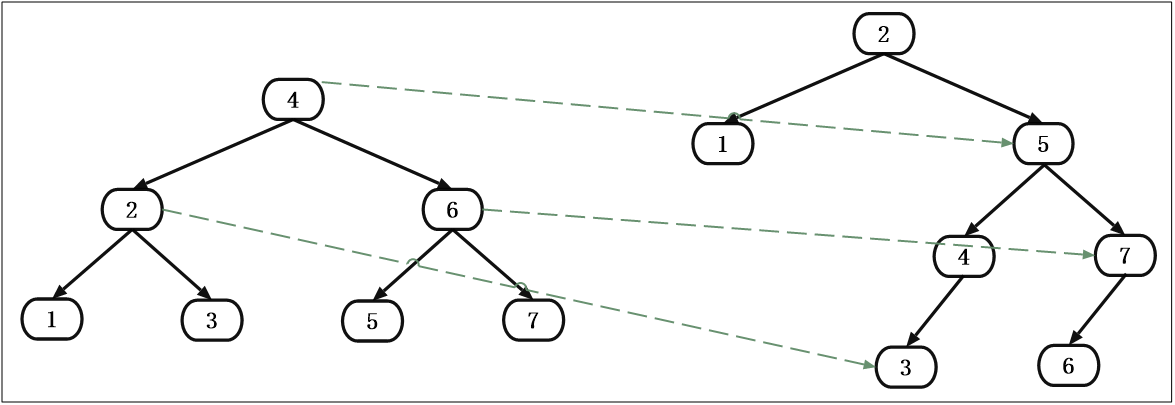
\includegraphics[width=1\textwidth]{Medien/Tango/transitionPoints}
	\caption{Transition point Zuordnung. Links ein Lower Bound Tree, rechts ein möglicher $T_j$.   }
	\label{fig:transitionPoints}
\end{figure}



\begin{Satz} \label{satzDemaine1}
	Sei $X = x_0, x_1,.., x_m$  eine Zugriffsfolge und $n$ die Anzahl der Knoten im zu $X$ erstellten Lower Bound Tree Y. Dann gilt\\	
	$\mathit{OPT}\left(X\right) \geq \mathit{IB}\left(X\right) /2 - n$ .
\end{Satz}
\begin{proof}
	Es wird die Mindestanzahl der Berührungen von transition points gezählt. Sei $U$ die Menge der Knoten von $Y$ mit einer nicht leeren rechten Region. Durch Lemma \ref{demaineLemma1} und Lemma \ref{lemmaDemaine3} kann die Anzahl der Berührungen für jeden Knoten $u \in U$ einzeln bestimmt werden. Diese müssen dann lediglich noch addiert werden. Sei $l$, $r$, $v_r$ und $v_l$ wie in Lemma \ref{demaineLemma1} zu $u$ definiert, so dass entweder $v_l$ oder $v_r$ der transition point zu $u$ sein muss, je nachdem welcher der beiden Knoten die größere Tiefe hat. Für $k \in \{1, 2,.., m\}$ sei \mbox{$X{^r_l}' = x_{i_0},x_{i_1},..,x_{i_p}$} die Folge, die entsteht, wenn aus $X^r_l$ alle $x_k$ entfernt werden, für die gilt, $x_k$ ist in der gleichen Region von $u$ wie $x_{k-1}$. Damit gilt $\mathit{inScore}\left(u\right) = p$. Nun wird angenommen, dass die $x_{i_j}$ mit, $j$ ist eine gerade Zahl, in der rechten Region von $u$ liegen und die $x_{i_j}$ mit, $j$ ist eine ungerade Zahl, in der linken Region. Der andere Fall kann wieder direkt abgeleitet werden. Sei $q \in \mathbb{N}$ mit $1 \leq q \leq \lfloor p / 2 \rfloor$. \textit{access}$\left( x_{i_{2q-1}} \right)$ muss $v_l$ berühren und \textit{access}$\left( x_{i_{2q}} \right)$ muss $v_r$ berühren. Sei $k_{1}$ der Schlüssel des transition point von $u$ zu Beginn von \textit{access}$\left( x_{i_{2q-1}} \right)$ und  $k_{2}$ der Schlüssel des transition point von $u$ zu Beginn von \textit{access}$\left( x_{i_{2q}} \right)$. Gilt $k_{1} = k_{2}$, so muss der transition point von $u$ in \textit{access}$\left( x_{i_{2q}} \right)$ berührt worden sein.  Gilt $k_{1} \ne k_{2}$, so muss der transition point von $u$ nach Lemma \ref{demaineLemma2} in \textit{access}$\left( x_{i_{2q-1}} \right)$ berührt worden sein. Aus der Konstruktion von $X{^r_l}'$ folgen daraus mindestens $\lfloor p/2 \rfloor \geq p/2 - 1$ Berührungen des transition point von $u$. \\
	Addieren über alle Knoten aus $U$ ergibt bei den Werten der $\mathit{inScore}$ Funktion die Interleave Lower Bound und bei den Berührungen von transition points zumindest  $\mathit{IB}\left(X\right) /2 - \vert U \vert \geq \mathit{IB}\left(X\right) /2 - n$.
	
\end{proof}


\subsection{Der Aufbau des Tango Baumes.} \label{aufbauDesTango}
Wie bereits erwähnt besteht ein Tango Baum $T$ aus Hilfsbäumen. Eine Anforderung an einen Hilfsbaum mit $n$ Knoten ist es, dass für seine Höhe $h = O\left(\log\left( n\right)\right)$ gilt. $T$ bietet lediglich eine \textit{access} Operation an. Ist $T$ also erst einmal für die  Schlüsselmenge $K$ erzeugt, ist diese unveränderlich. Sei $P$ der Lower Bound Tree aus Abschnitt \ref{interBound} mit der Schlüsselmenge $K$. $P$ wird auch als \textbf{Referenzbaum} für $T$ bezeichnet. $P$ ist kein Hilfsbaum und muss in Implementierungen auch nicht erstellt werden. Er dient aber dazu, den Aufbau von $T$ vor und nach einer \textit{access} Operation zu veranschaulichen. Jeder innere Knoten $p$ in $P$ kann ein \textbf{preferred child} haben.  Wurde während der Ausführungszeit von $X$ noch keine \textit{access} Operation mit einem im Teilbaum mit der Wurzel $p$ enthalten Schlüssel als Parameter ausgeführt, so hat $p$ kein preferred child. Ansonsten sei \textit{access}$\left(k\right)$ die zuletzt ausgeführte Operation mit einem Schlüssel, der im Teilbaum mit der Wurzel $p$ enthalten ist. Ist $k$ in der linken Region von $p$ enthalten, dann ist das linke Kind von $p$ das preferred child von $p$. Ist $k$ in der rechten Region von $p$ enthalten, dann ist das rechte Kind von $p$, das preferred child von $p$. Wir erweitern die Knoten von $P$ mit einer weiteren Variable \textit{prefChild}, welche drei Werte annehmen kann. Sie enthält \textit{none}, wenn ihr Knoten kein preferred child besitzt, \textit{left}, wenn das linke Kind das preferred child ist, ansonsten entsprechend \textit{right}. Hier ist bereits die Kopplung zur Interleave Lower Bound erkennbar. Ein Wechsel von \textit{prefChild}  von \textit{left} zu \textit{right} oder umgekehrt, findet genau dann statt, wenn es zu einem interleave durch den Knoten kommt. Abbildung \ref{fig:prefChilds} stellt einen möglichen Zustand von $P$ zwischen zwei \textit{access} Operationen dar. Dieser Zustand wird in diesem Abschnitt nun als durchgängiges Beispiel dienen. Es ist sofort ersichtlich, dass der Parameter der letzten \textit{access} Operation $8$, $4$, $2$ oder $1$ gewesen sein muss, da die Knoten mit diesen Schlüsseln von der Wurzel aus über preferred children erreichbar sind. Die Schlüssel $10$ und $9$ können noch nie Parameter einer \textit{access} Operation gewesen sein. Ansonsten müsste der Knoten mit dem Schlüssel $10$ ein preferred child haben. Mit Hilfe der preferred children lassen sich die \textbf{preferred path} erstellen. Sei $v$ ein Knoten in $P$, der nicht das preferred child eines anderen Knotens aus $P$ ist. Dann ist der preferred path zu $v$, der längst mögliche Pfad $\left(v_0, v_1,..,v_l\right)$, mit $v_0 = v$ und $\forall i \in \{1,2,..,l\} \colon v_i \textit{ ist das preferred child von }v_{i-1   }$.  

\begin{figure}[H]
	\centering
	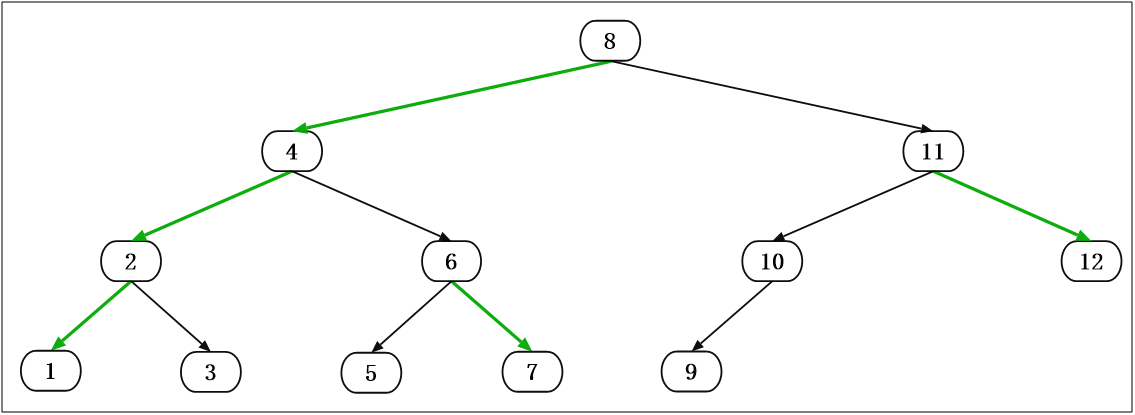
\includegraphics[width=1\textwidth]{Medien/Tango/prefChilds}
	\caption{Die preferred children im Referenzbaum werden durch die grünen Pfeile markiert. }
	\label{fig:prefChilds}
\end{figure}

\noindent Nun werden die preferred path des BST aus Abbildung \ref{fig:prefChilds} angegeben, wobei der Schlüssel jeweils als Bezeichner für den ihn enthaltenden Knoten verwendet wird.
\begin{align*}
&P_1 =  \left( 8, 4, 2,1 \right) \\
&P_2 = \left(3 \right)\\
&P_3 = \left(6, 7 \right)\\
&P_4 = \left(5 \right)\\
&P_5 = \left(11, 12 \right) \\
&P_6 = \left(10 \right)\\
&P_7 = \left(9\right)
\end{align*}

\noindent Da jeder Knoten nur das preferred child eines Knotens sein kann und Knoten die kein preferred child sind als Startknoten eines Pfades dienen, muss jeder Knoten in genau einem preferred path enthalten sein.\\
Zu jedem preferred path gibt es einen Hilfsbaum, der genau die Schlüssel enthält, die in den Knoten des Pfades enthalten sind. Da der Tango Baum den inneren Aufbau der Hilfsbäume nicht exakt vorschreibt, zeigt \mbox{Abbildung \ref{fig:Hilfsbäume}} nur eine mögliche Konstellation.


\begin{figure}[H]
	\centering
	\includegraphics[width=1\textwidth]{Medien/Tango/Hilfsbäume}
	\caption{Die Hilfsbäume zu den preferred path aus dem Beispiel. }
	\label{fig:Hilfsbäume}
\end{figure}
\noindent Sei $H$ die Menge der erstellten Hilfsbäume aus $P$. Mit dem folgenden Verfahren können Hilfsbäume zu einem Tango Baum zusammengefügt werden:
\begin{enumerate}
	\item Gilt $\vert H \vert = 1$, dann ist das in $H$ enthaltene Element der Tango Baum und es wird abgebrochen.
	\item Wähle $h_1 \in H$ so, dass $h_1$ nicht den Schlüssel der Wurzel von $P$ enthält.
	\item Aufgrund der Konstruktion der preferred paths muss es genau einen Knoten $v$ in $h_1$ geben, so dass der Knoten $u$ in $P$ mit $\mathit{key}\left(v\right) = \mathit{key}\left(u\right) $ nicht das preferred child seines Elternknotens ist.
	Sei $h_2$ der Hilfsbaum, der den Schlüssel des Elternknotens von $u$ enthält. Entferne $h_1$ und $h_2$ aus $H$.
	\item Sei $w_1$ die Wurzel von $h_1$. Sei $a$ der Knoten in $h_2$, an dem die Standardvariante von \textit{insert} einen für Schlüssel  $\mathit{key\left(w_1\right)}$ erzeugten Knoten anfügen würde. Dann wird $h_1$ an $a$ angefügt. Aufgrund der Links-Rechts-Beziehung in BST kann es nur eine Möglichkeit dafür geben. Sei $h_3$ der so entstandene BST.
	\item Füge $h_3$ zu $H$ hinzu, weiter mit $1$.
\end{enumerate}

\noindent Bei Punkt $4$ ist sofort ersichtlich, dass es durch $\mathit{key}\left(w_1\right)$ zu keiner Verletzung der Links-Rechts-Beziehung kommt. Wie sieht es aber mit den anderen Schlüsseln aus $h_1$ aus ? \\
In $P$ sind alle in $h_1$ enthaltenen Schlüssel im Teilbaum mit der Wurzel $u$ enthalten. Sei $l$ der kleinste Schlüssel in diesem Teilbaum und $r$ der größte. In $P$ kann es außerhalb des Teilbaumes mit der Wurzel $u$ keinen Schlüssel $k$ mit $l \leq k \leq r$ geben. $h_2$ kann nur Schlüssel enthalten, die kleiner $l$ oder größer $r$ sind. Im Tango Baum kann es also keine Verletzung der Links-Rechts-Beziehung geben.\\


\noindent Abbildung \ref{fig:Tangobaum} zeigt unseren Tango Baum $T$ zum Beispiel. Die Wurzeln von Hilfsbäumen sind grün dargestellt.

\begin{figure}[H]
	\centering
	\includegraphics[width=1\textwidth]{Medien/Tango/Tangobaum}
	\caption{Der Tango Baum zu dem Beispiel. }
	\label{fig:Tangobaum}
\end{figure}
\noindent Nehmen wir an, dass auf $T$ \textit{access}$\left(9\right)$ ausgeführt wird. Abbildung \ref{fig:prefChilds2} zeigt den Zustand von $P'$.

\begin{figure}[H]
	\centering
	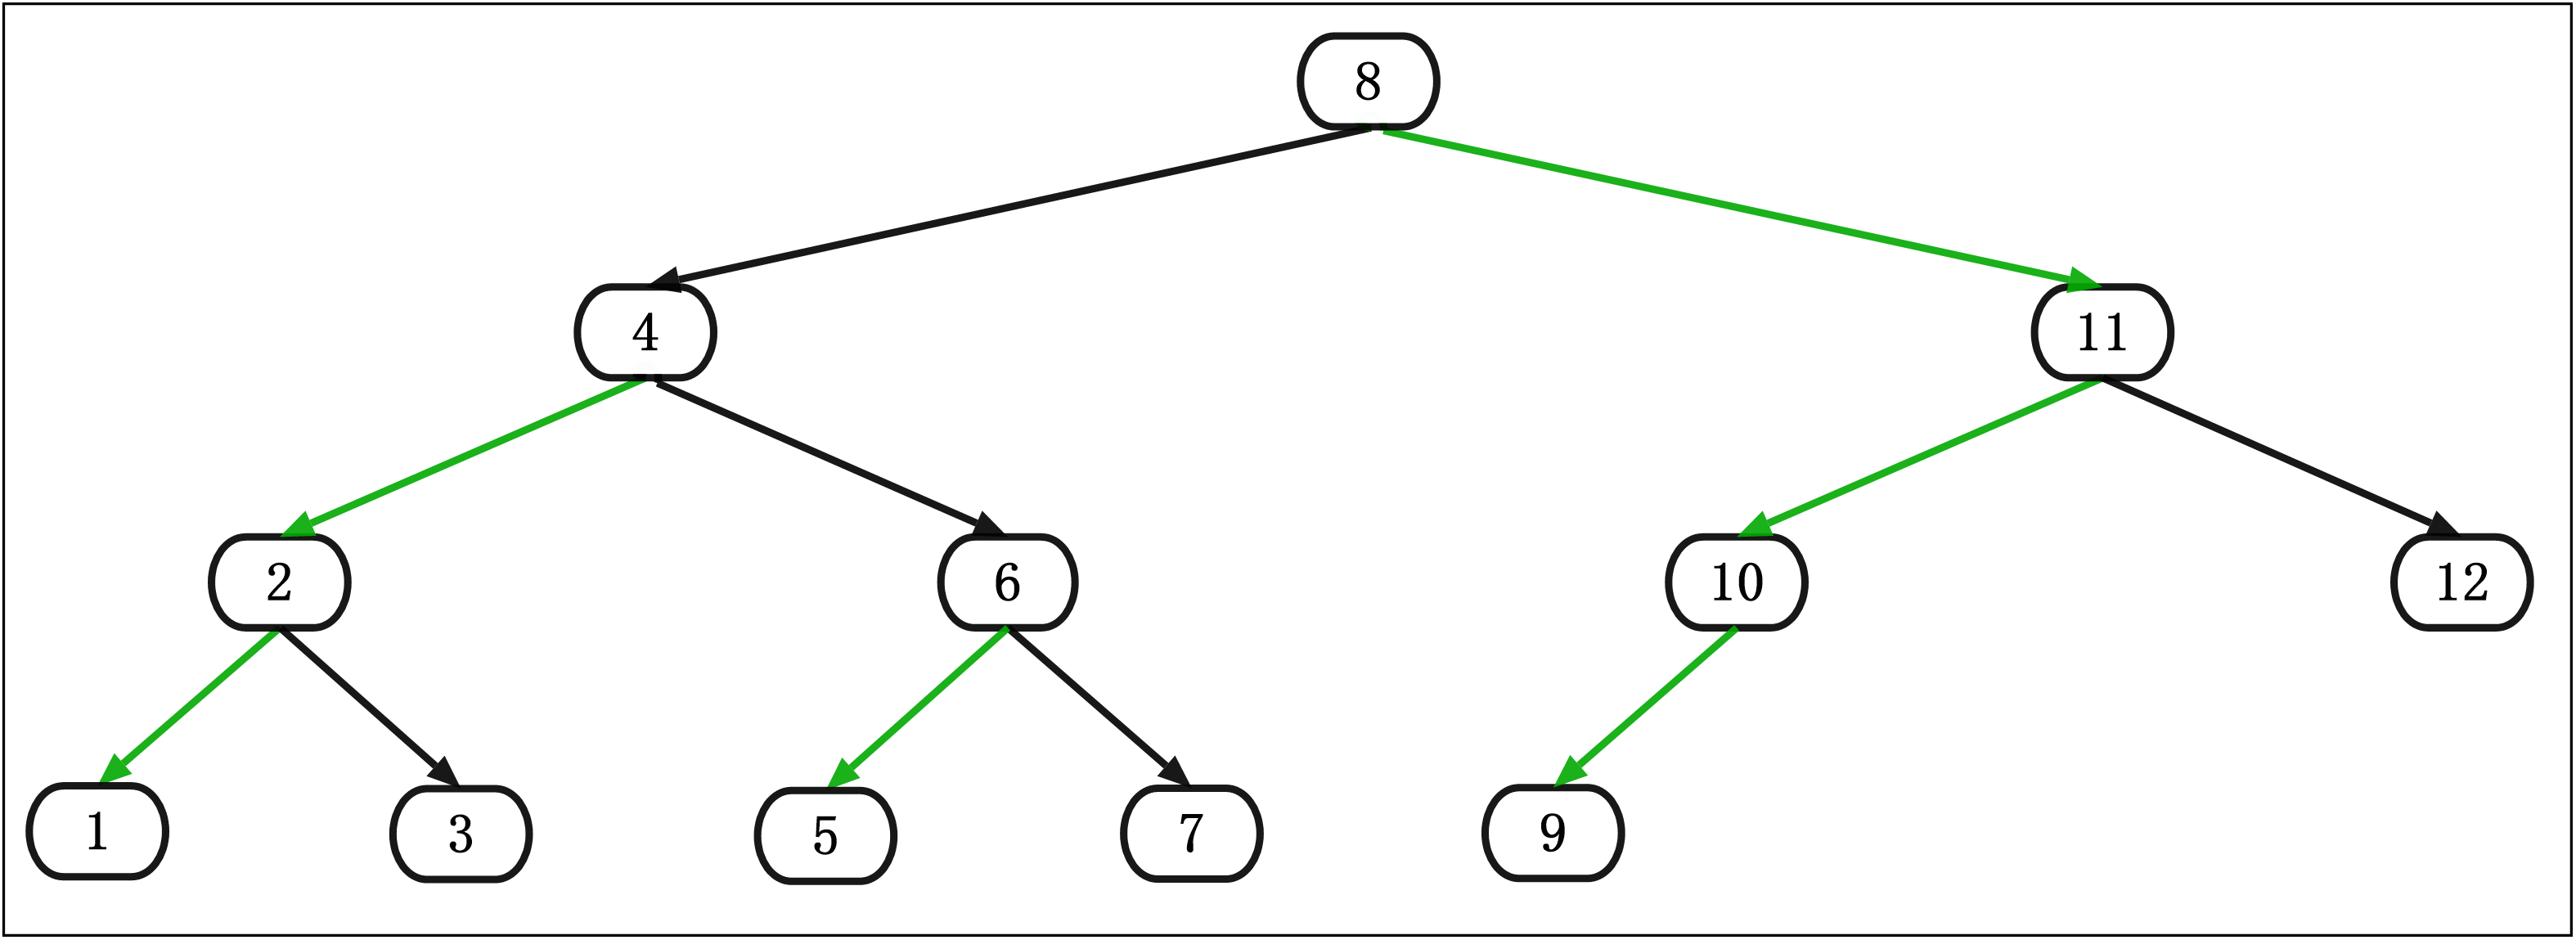
\includegraphics[width=1\textwidth]{Medien/Tango/prefChilds2}
	\caption{Die preferred children nachdem  \textit{access}$\left(9\right)$ ausgeführt wurde. }
	\label{fig:prefChilds2}
\end{figure}

\noindent Abbildung \ref{fig:Tangobaum2} zeigt einen möglichen Zustand von $T'$.
\begin{figure}[H]
	\centering
	\includegraphics[width=1\textwidth]{Medien/Tango/Tangobaum2}
	\caption{Der Tango Baum nachdem  \textit{access}$\left(9\right)$ ausgeführt wurde. }
	\label{fig:Tangobaum2}
\end{figure}
\noindent Im nächsten Abschnitt wird es vor allem darum gehen, wie eine Transformation, wie die von $T$ zu $T'$, effizient durchgeführt werden kann.

\subsection{Die \textit{access} Operation beim Tango Baum.}
Die Knoten in einem Tango Baum sind mit zusätzlichen Daten erweitert. Sei $v$ ein Knoten im Tango Baum. Es gibt eine boolesche Variable \textit{isRoot}, die genau dann den Wert \textit{true} annimmt, wenn $v$ die Wurzel eines Hilfsbaumes ist. In einer Konstante \textit{depth} wird die Tiefe des Knotens mit dem Schlüssel $\mathit{key}\left(v\right)$ in $P$ gespeichert. Außerdem gibt es noch die Variablen \textit{minDepth} und \textit{maxDepth}. Sei $v$ im Hilfsbaum $H$ enthalten und sei $H_v$ der Teilbaum mit der Wurzel $v$ in $H$. Da $H$ die Schlüssel von Knoten aus einem preferred path enthält, können die \textit{depth} Konstanten zweier Knoten in $H$ nicht den gleichen Wert haben. Sei $\mathit{min}$ der kleinste Wert aller \textit{depth} Konstanten in $H_v$, dann entspricht $\mathit{min}$ dem  Wert der \textit{minDepth} Variable von $v$. Sei $\mathit{max}$ der größte Wert aller \textit{depth} Konstanten in $H_v$, dann entspricht $\mathit{max}$ dem  Wert der \textit{maxDepth} Variable von $v$. Auf die Variablen und Konstanten eines Knoten $v$ wird im Folgenden mit dem Punkt als Trennzeichen zugegriffen, \mbox{z. B.} $v$.\textit{depth}. \\
Nun werden die Anforderungen an einen Hilfsbaum $H$ aufgezählt:
\begin{enumerate}
	\item Sei $n$ die Anzahl der Knoten von $H$. Für die Höhe $h$ von $H$ gilt \mbox{$h = O\left(\log \left(n\right)\right)$}.
	\item $H$ aktualisiert seine Zeiger auf andere Hilfsbäume.
	\item $H$ aktualisiert die Variablen  \textit{minDepth} und \textit{maxDepth}.
	\item $H$ bietet eine Operation \textit{concatenate(HB $H_1$, Node $v_k$, HB  $H_2$)} an. HB ist eine Abkürzung für Hilfsbaum. Bei maximal einem \textit{HB}  darf die \textit{isRoot} Variable der Wurzel den Wert \textit{true} haben. Sei $K_1$ die Schlüsselmenge von $H_1$, $K_2$ die Schlüsselmenge von $H_2$ und $k$ der Schlüssel von $v_k$. Die Operation kann verwenden, dass für $k_1 \in K_1$ und $k_2 \in K_2$, $k_1 < k < k_2$ gilt. Es werden drei Fälle unterschieden. Sei $w_1$ die Wurzel von $H_1$ und $w_2$ die von $H_2$.
	\begin{enumerate}
		\item $w_1$.\textit{isRoot} $=$ \textit{false} und $w_2$.\textit{isRoot} $=$ \textit{false}:\\
		Die Operation gibt die Wurzel eines Hilfsbaumes $H$ mit der Schlüsselmenge $K_1 \cup K_2 \cup \{k\} $ zurück.
		\item $w_1$.\textit{isRoot} $=$ \textit{true}:\\	
		Die Operation gibt die Wurzel eines Hilfsbaumes $H$ mit der Schlüsselmenge $K_2 \cup \{k\} $ zurück. An $H$ ist ein Hilfsbaum $H_3$ mit der Schlüsselmenge $K_1$ angefügt. Die \textit{isRoot} Variable der Wurzel von $H_3$ hat den Wert \textit{true}.
		\item $w_2$.\textit{isRoot} $=$ \textit{true}:\\	
		Die Operation gibt die Wurzel eines Hilfsbaumes $H$ mit der Schlüsselmenge $K_1 \cup \{k\} $ zurück. An $H$ ist ein Hilfsbaum $H_3$ mit der Schlüsselmenge $K_2$ angefügt. Die \textit{isRoot} Variable  der Wurzel von $H_3$ hat den Wert \textit{true}.	 
	\end{enumerate}
	In allen Fällen hat die \textit{isRoot} Variable der Rückgabe den Wert \textit{false}.
	Für die Laufzeit der Operation muss $O\left(\log \left(\vert K_1 \vert + \vert K_2 \vert\right)\right)$ gelten.
	\item $H$ bietet eine Operation \textit{split}$($key $k)$ an. Die Operation kann verwenden, dass in $H$ ein Knoten mit dem Schlüssel $k$ existiert. Sei $K$ die Schlüsselmenge von $H$. Die Operation gibt einen Knoten $v$ mit dem Schlüssel $k$ zurück. Das linke Kind von $v$ muss die Wurzel eines Hilfsbaumes mit der Schlüsselmenge ${K_l=\{i\in K \mid  i <k\}}$ sein. Das rechte Kind von $v$ muss die Wurzel eines Hilfsbaumes mit der Schlüsselmenge ${K_r=\{i\in K \mid  i > k\}}$ sein. Die  \textit{isRoot} Variablen von $v$ und dessen Kindern haben den Wert \textit{false}. Für die Laufzeit der Operation muss $O\left(\log \left(\vert K \vert\right) \right)$ gelten.
\end{enumerate} 
Jetzt werden noch zwei Hilfsoperationen vorgestellt, die für \textit{access} benötigt werden.\\

\paragraph{cut Operation:} \label{cut}

\noindent \textit{cut(depth $d$)} zerteilt einen Hilfsbaum $A$ in zwei Hilfsbäume. Es dürfen nur Werte für $d$ übergeben werden, zu denen es in $A$ einen Knoten $v$ mit $v.$\textit{depth} $ = d $ gibt. Die Rückgabe ist ein Hilfsbaum $G$ mit den Schlüsseln der Knoten mit \textit{depth} $\leq d$ in $A$. An $G$ ist ein Hilfsbaum mit den restlichen Schlüsseln aus $A$ angefügt. Zunächst werden die Knoten mit den Schlüsseln $l$,  $l'$, $r$ und $r'$ in $A$ gesucht. $l$ ist der kleinste Schlüssel eines Knotens $v_l$ in $A$, mit $v_l$.\textit{depth} $> d$. $r$ ist der größte Schlüssel eines Knotens $v_r$ in $A$, mit $v_r$.\textit{depth} $> d$. $l'$ ist der Schlüssel des Vorgängers von $v_l$ und $r'$ der Schlüssel des Nachfolgers von $v_r$. $l$ und $r$ müssen in $A$ enthalten sein, $l'$ und $r'$ könnten auch fehlen. $v_l$ kann wie folgt gefunden werden:\\ Zu Beginn wird der Zeiger $p$ auf die Wurzel von $A$ gesetzt. Zeigt $p$ nicht auf $v_l$, muss es im linken Teilbaum von $p$ einen Knoten $v$ mit $v$.\textit{depth} $> d$ geben. Dies ist an der \textit{maxDepth} Variable des linken Kindes von $p$ direkt abfragbar. Ist $v_l$ erreicht, kann $l'$ über eine Suche nach dem Vorgänger von $v_l$ gefunden werden. Die Suche nach $r$ und $r'$ verläuft analog. \\
$A$ besteht aus Schlüsseln aus einem preferred path. Somit muss für jeden Schlüssel $k$ eines Knotens $v$ mit $v$.\textit{depth} $\leq d$ in $A$ entweder $k > r$ oder $k < l$ gelten, denn alle Schlüssel aus $\left[l,r\right]$ liegen in $P$ entweder im linken oder im rechten Teilbaum des Knotens mit dem Schlüssel $k$. \\
Es wird nun der Ablauf von \textit{cut} gezeigt. Wobei angenommen wird, dass sowohl $l'$ als auch $r'$ existieren. Die anderen Fälle können einfach abgeleitet werden.
\begin{enumerate}
	\item Sei $w_a$ die Wurzel von $A$. Setze $w_a$.\textit{isRoot} auf \textit{false}. 
	\item Führe \textit{split}$\left(l'\right)$ auf $A$ aus. Sei $v_l$ die Rückgabe von \textit{split}$\left(l'\right)$. Sei $B$ der linke Teilbaum von $v_l$ und $C$ der Rechte. 
	\item Führe \textit{split}$\left(r'\right)$ auf $C$ aus. Sei $v_r$ die Rückgabe von \textit{split}$\left(r'\right)$. Sei $D$ der linke Teilbaum von $v_r$ und $E$ der Rechte. 
	\item Setze $v_r$ als das rechte Kind von $v_l$. 
	\item Setze die \textit{isRoot} Variable der Wurzel von $D$ auf \textit{true}.
	\item Führe $w_F = \textit{concatenate}\left(D, ~ v_r, ~ E \right)$ aus. Sei $F$ der Hilfsbaum von dem $w_F$ die Wurzel ist.
	\item Führe $w_G = \textit{concatenate}\left(B, ~ v_l,~ F \right)$ aus. Sei $G$ der Hilfsbaum von dem  $w_G$ die Wurzel ist.
	\item Setze die \textit{isRoot} Variable der Wurzel von $G$ auf \textit{true}.
\end{enumerate}
Nach der Operation ist die Wurzel von $G$ auch immer die Wurzel des Tango Baumes. Abbildung \ref{fig:cut} demonstriert den Ablauf nochmals und Abbildung \ref{fig:cut2} zeigt einen verkürzten Ablauf bei fehlendem $r'$.
\begin{figure}[H]
	\centering
	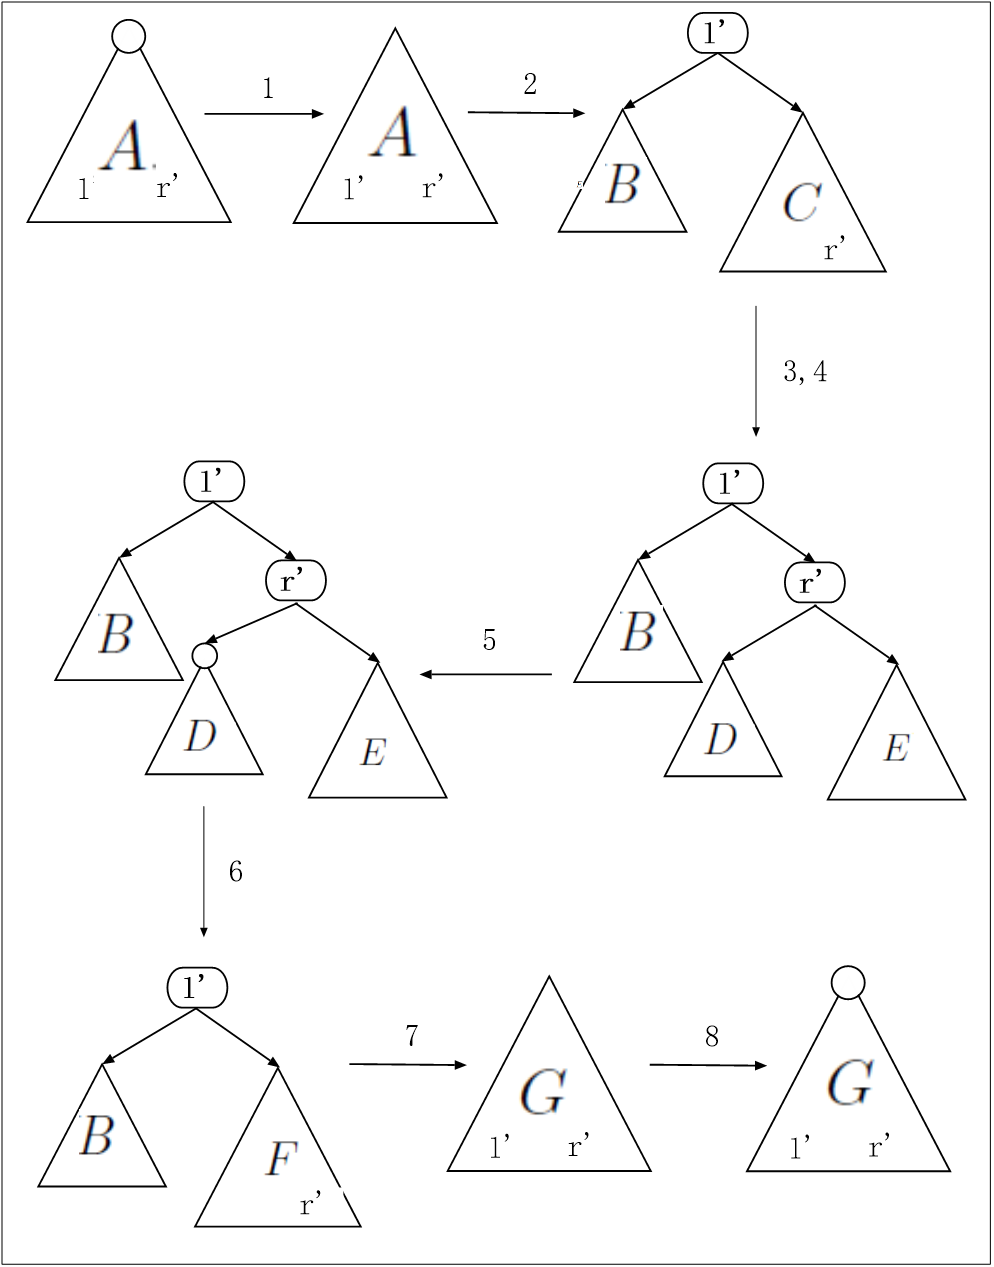
\includegraphics[width=1\textwidth]{Medien/Tango/cut}
	\caption{Ablauf von \textit{cut($d$)}. Die Abbildung basiert auf einer aus \cite{demainDinamicOpti}. Die Wurzeln von Hilfsbäumen sind mit einem Kreis markiert. }
	\label{fig:cut}
\end{figure}
\begin{figure}[H]
	\centering
	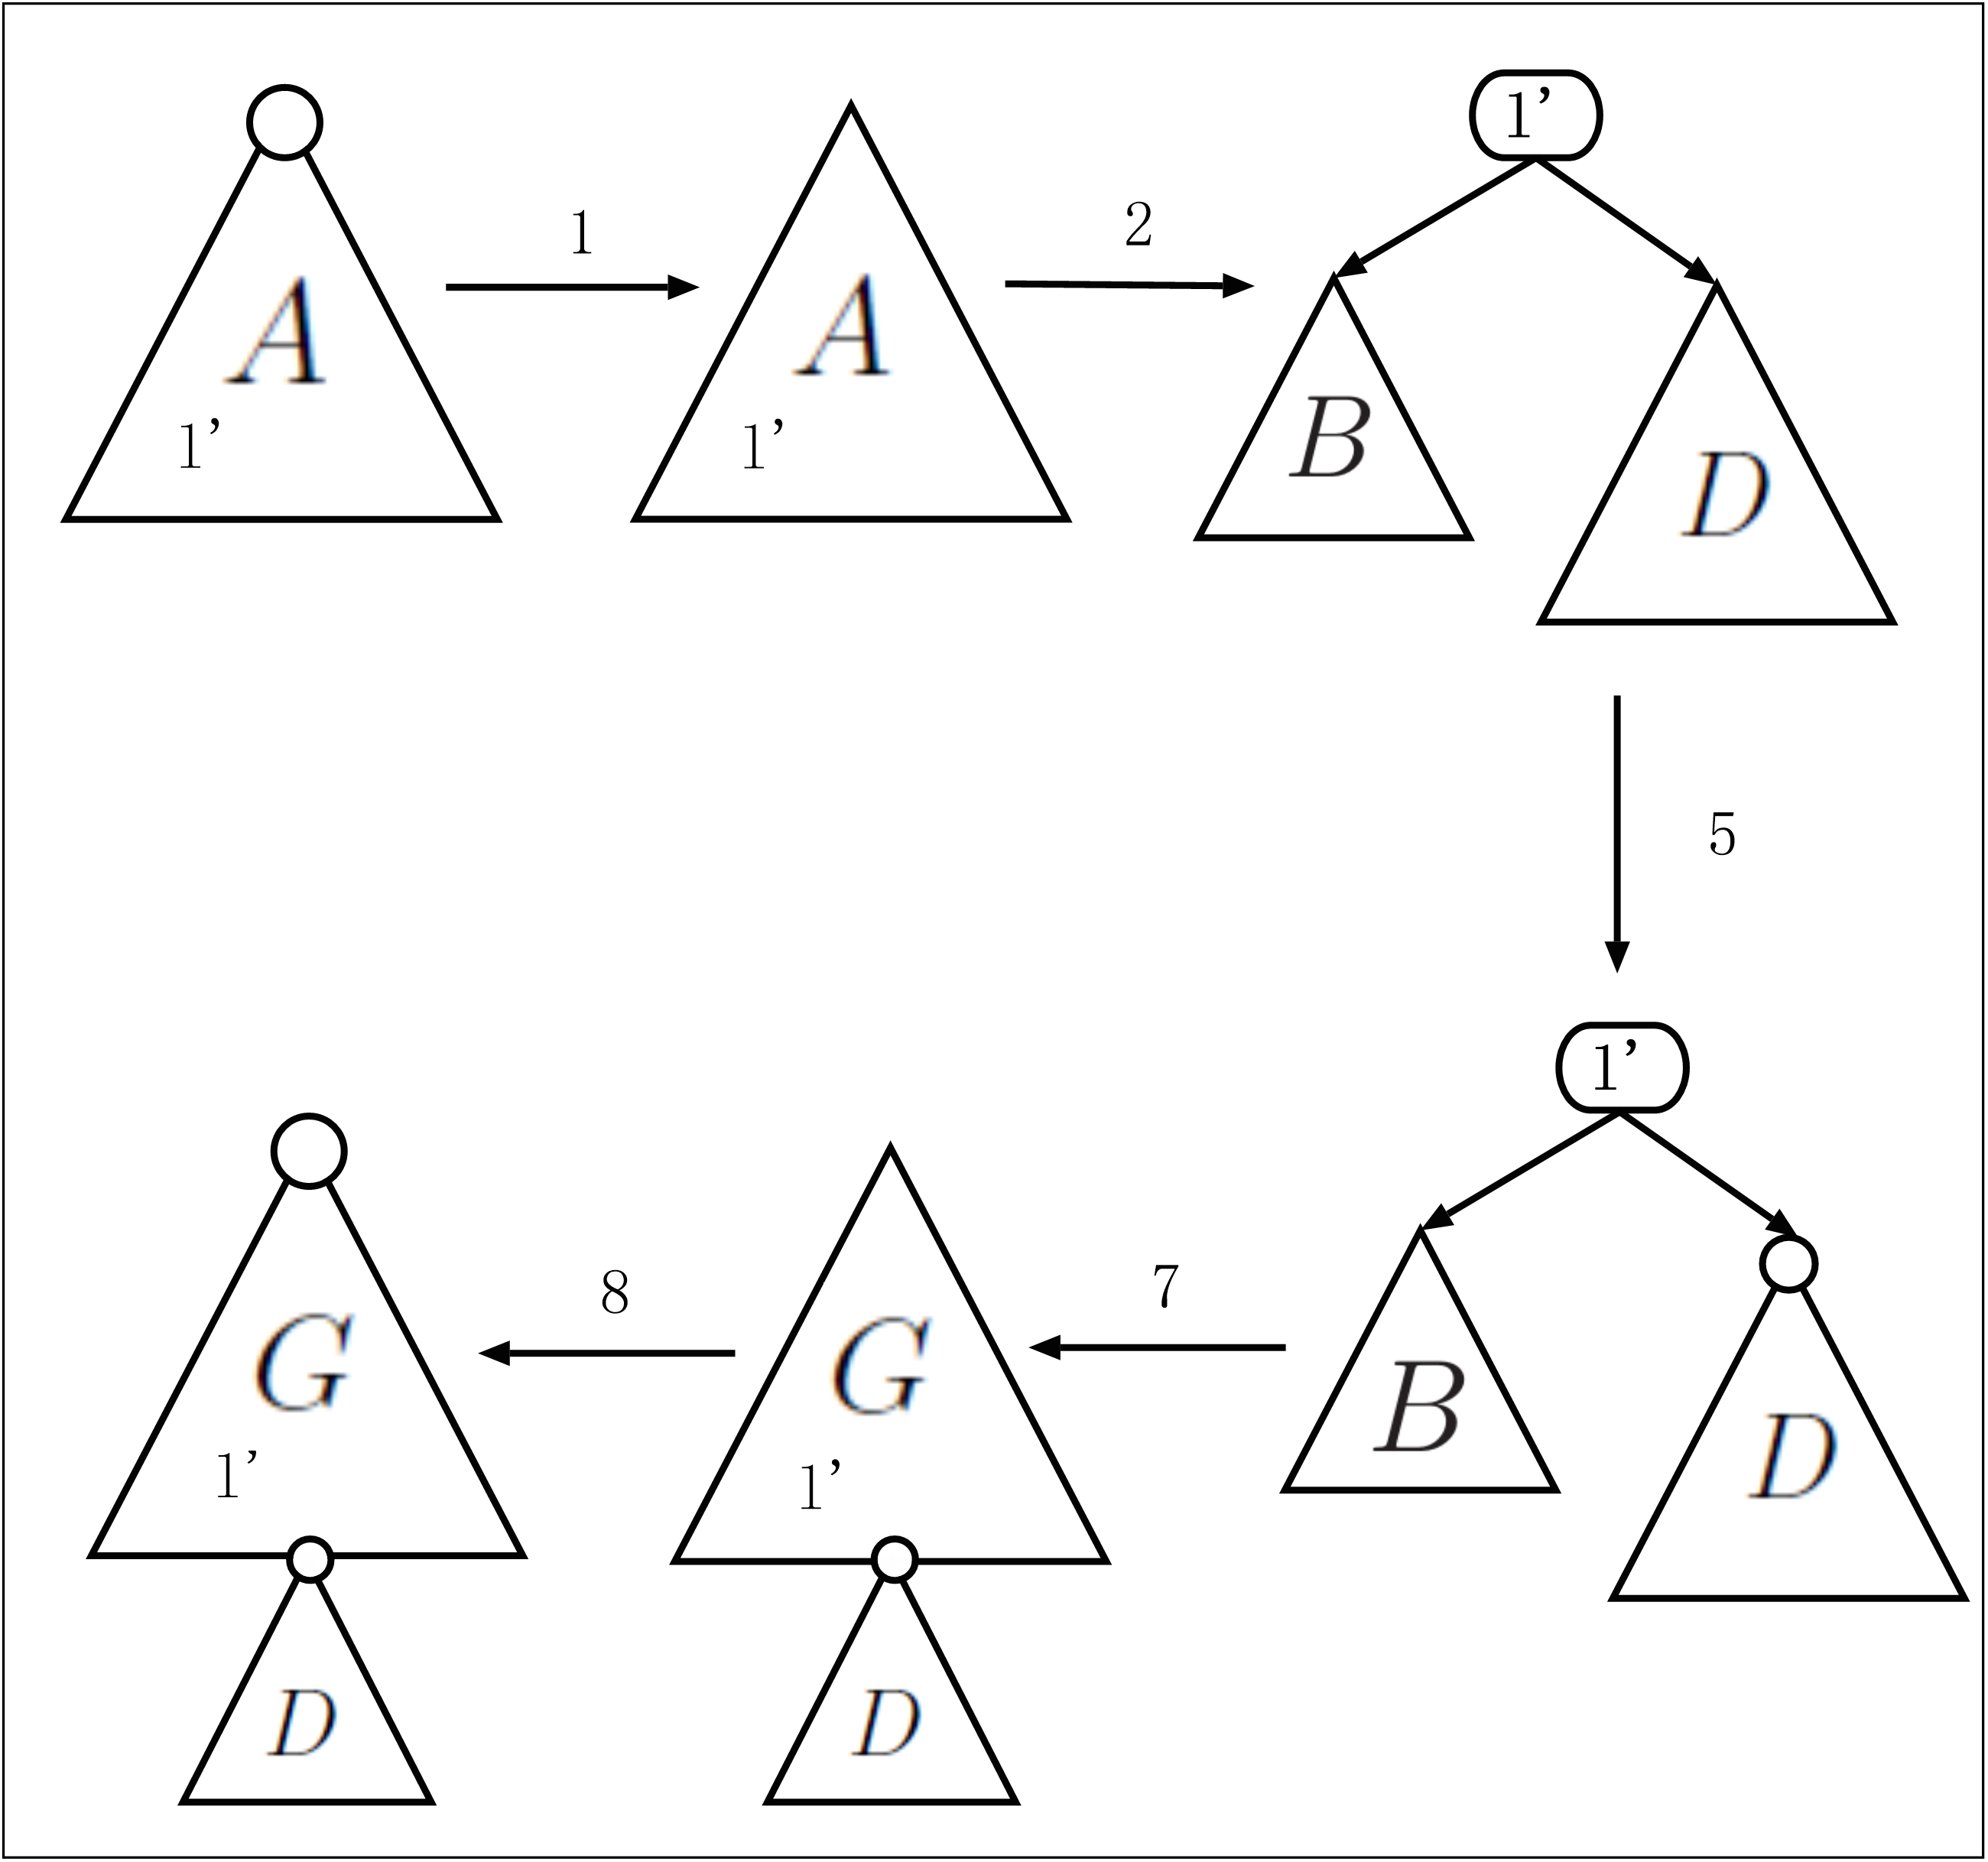
\includegraphics[width=1\textwidth]{Medien/Tango/cut2}
	\caption{Ablauf von \textit{cut($d$)} bei fehlenden $r'$. Die Abbildung basiert auf einer aus \cite{demainDinamicOpti}. Die Wurzeln von Hilfsbäumen sind mit einem Kreis markiert. }
	\label{fig:cut2}
\end{figure}
\noindent Sei $n$ die Anzahl der Knoten von $A$. Jeder der acht Schritte kann in $O\left(\log \left(n\right)\right)$ Zeit ausgeführt werden. Somit gilt auch für die Gesamtlaufzeit $O\left(\log \left(n\right)\right)$.


\paragraph{join Operation:}
\noindent \textit{join}$($HB $H_1$, HB $H_2)$ fügt die Hilfsbäume $H_1$ und $H_2$ zu einem Hilfsbaum $H$ zusammen. Auch $H$ repräsentiert wieder einen preferred path. Es muss also möglich sein einen Pfad im Referenzbaum zu bilden, der genau die Knoten mit den Schlüsseln aus $H_1$ und $H_2$ enthält.\\ 
Sei $v_1$ die Wurzel von $H_1$ und $v_2$ die von $H_2$. Es muss \\ $v_1$.\textit{maxDepth} $+ 1$ =  $v_2$.\textit{minDepth} gelten. Auch hier werden Schlüssel $l$, $l'$, $r$ und $r'$ verwendet. Sei $l$ der kleinste Schlüssel in $H_2$ und $r$ der größte Schlüssel in $H_2$. 
Für jeden Schlüssel $k$ in $H_1$ muss entweder $k < l$ oder $k > r$ gelten. $l'$ ist der größte Schlüssel in $H_1$ mit $l' < l$. $r'$ ist der kleinste Schlüssel in $H_1$ mit $r' > r$. Wird in $H_1$ ein Schlüssel aus $H_2$ gesucht, so muss die Suche entweder bei $l'$, bzw. $r'$ erfolglos enden. Der andere Schlüssel kann dann mit einer Suche nach dem Nachfolger, bzw. Vorgänger gefunden werden. Der Ablauf von \textit{join} ist dem von \textit{cut} recht ähnlich. Wieder wird angenommen, dass $l'$ und $r'$ existieren.
\begin{enumerate}
	\item Sei $w_1$ die Wurzel von $H_1$ und $w_2$ die von $H_2$. Setze $w_1$.\textit{isRoot} und  $w_2$.\textit{isRoot} auf \textit{false}.
	\item Führe \textit{split}$\left(l'\right)$ auf $H_1$ aus. Sei $v_l$ die Rückgabe von \textit{split}$\left(l'\right)$. Sei $B$ der linke Teilbaum von $v_l$ und $C$ der Rechte. 
	\item Führe \textit{split}$\left(r'\right)$ auf $C$ aus. Sei $v_r$ die Rückgabe von \textit{split}$\left(r'\right)$. Sei $E$ der rechte Teilbaum von $v_r$. Der linke Teilbaum von $v_r$ muss der leere Baum sein. 
	\item Setze $v_r$ als das rechte Kind von $v_l$. Setze die Wurzel von $H_2$ als das linke Kind von $v_r$.
	\item Führe $w_F = \textit{concatenate}\left(H_2, ~ v_r, ~ E \right)$ aus. Sei $F$ der Hilfsbaum von dem $w_F$ die Wurzel ist.
	\item Führe $w_H = \textit{concatenate}\left(B, ~ v_l,~ F \right)$ aus. Sei $H$ der Hilfsbaum von dem $w_H$ die Wurzel ist.
	\item Setze die \textit{isRoot} Variable der Wurzel von $H$ auf \textit{true}.
\end{enumerate}
Nach der Operation ist die Wurzel von $H$ auch immer die Wurzel des Tango Baumes. Abbildung \ref{fig:join} demonstriert den Ablauf nochmals und Abbildung \ref{fig:join2} zeigt einen verkürzten Ablauf bei fehlendem $r'$.
\begin{figure}[H]
	\centering
	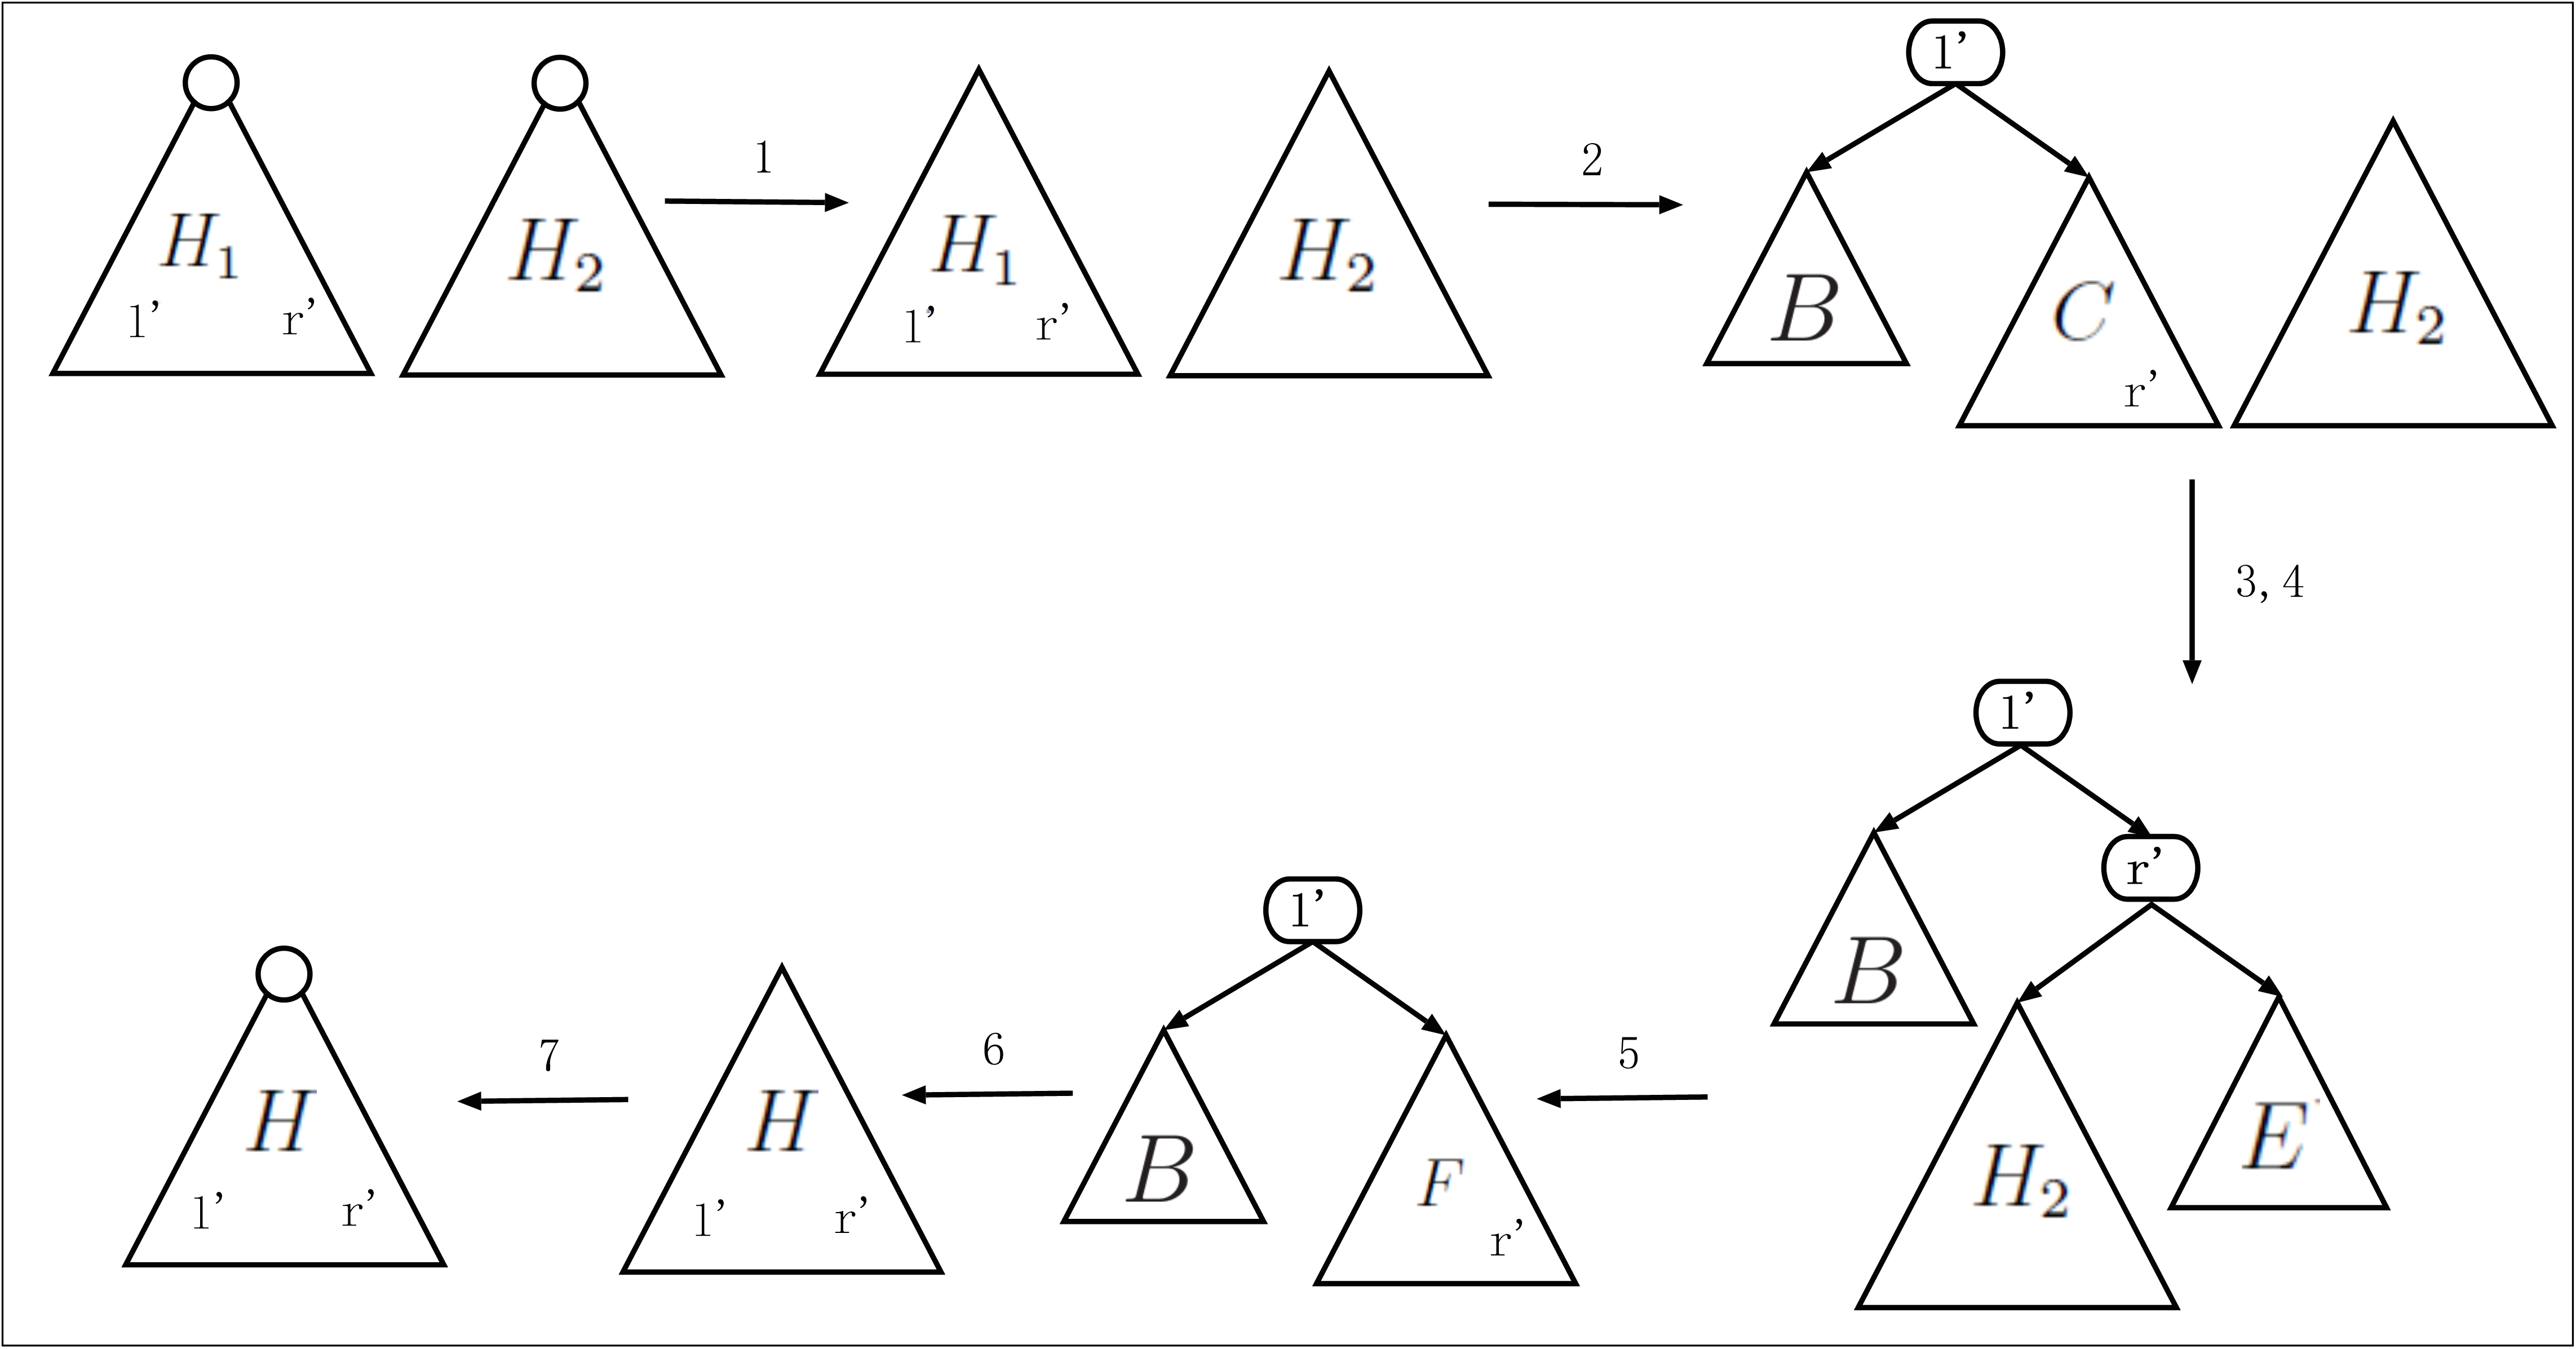
\includegraphics[width=1\textwidth]{Medien/Tango/join}
	\caption{Ablauf von \textit{join}$(H_1, H_2)$. Die Abbildung basiert auf einer aus \cite{demainDinamicOpti}. Die Wurzeln von Hilfsbäumen sind mit einem Kreis markiert }
	\label{fig:join}
\end{figure}
\begin{figure}[H]
	\centering
	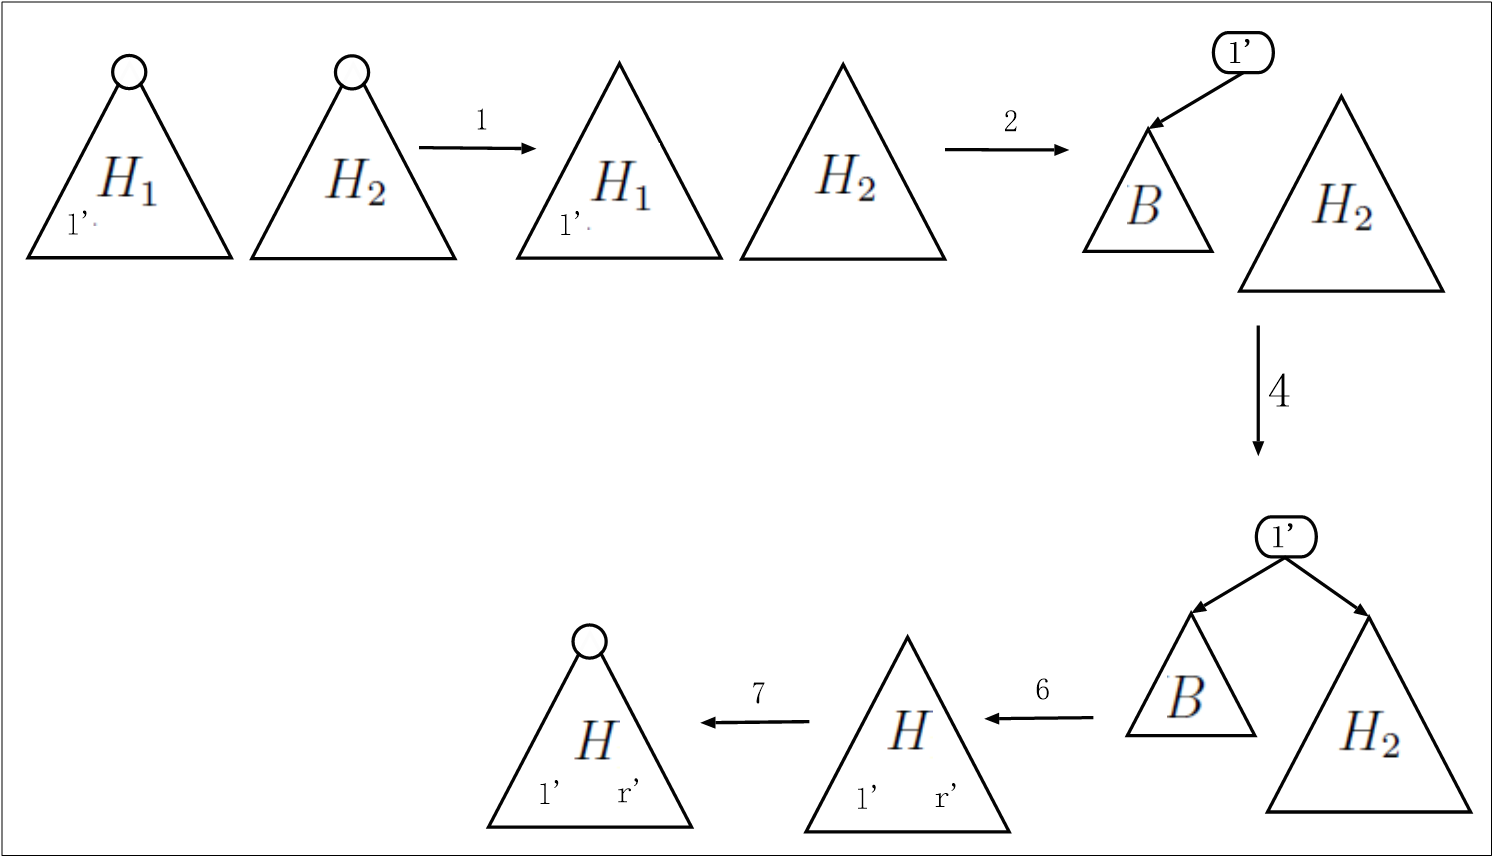
\includegraphics[width=1\textwidth]{Medien/Tango/join2}
	\caption{Ablauf von  \textit{join}$(H_1, H_2)$ bei fehlendem $r'$. Die Abbildung basiert auf einer aus \cite{demainDinamicOpti}. Die Wurzeln von Hilfsbäumen sind mit einem Kreis markiert. }
	\label{fig:join2}
\end{figure}

\noindent Sei $n$ die Anzahl der Knoten von $H$. Jeder der sieben Schritte kann in $O\left(\log \left(n\right)\right)$ Zeit ausgeführt werden. Somit gilt auch für die Gesamtlaufzeit $O\left(\log \left(n\right)\right)$.
\paragraph{access Operation:}
Nun wird die \textit{access} Operation des Tango Baumes betrachtet. Sei $k$ der Parameter der Operation und $p$ der Zeiger der Operation in den BST. Solange $p$ auf einen Knoten zeigt, der sich im Hilfsbaum mit der Wurzel des Tango Baumes $T$ befindet, verhält sich die Operation wie die Standardvariante von \textit{search}. Erreicht $p$ die Wurzel eines anderen Hilfsbaumes $H_2$, muss sich ein preferred child in $P$ verändert haben. $T$ wird mit \textit{cut} und \textit{join} so angepasst, dass er wieder die preferred paths in $P$ repräsentiert. Anschließend startet $p$ wieder an der Wurzel von $T$. Erreicht $p$ den Knoten mit dem Schlüssel $k$, wird das preferred child des Knotens mit dem Schlüssel $k$ in $P$ auf \textit{left} gesetzt. Daher kann nochmals eine Anpassung notwendig sein. Die Operation wird noch detaillierter beschrieben. Zur Vereinfachung bezeichnet $T$ immer den aktuellen Zustand des Tango Baumes und $H_1$ immer den Hilfsbaum mit der Wurzel von $T$:
\begin{enumerate}
	\item Setze $p$ auf die Wurzel von $H_1$.
	\item Suche nach $k$. Wird $k$ innerhalb von $H_1$ erreicht, weiter bei \ref{gefunden}. Ansonsten wird die Wurzel eines Hilfsbaumes $H_2$ erreicht.
	\item Sei $w_2$ die Wurzel von $H_2$. Führe $H_3 =$ \textit{cut}$\left(w_2.\textit{minDepth} - 1\right)$ auf $H_1$ aus.
	\item Führe \textit{join}$\left(H_3, ~H_2\right)$ aus. Weiter bei 1.
	\item \label{gefunden} Sei $v$ der Knoten mit \textit{key}$\left(v\right) = k$. Führe $H_4=$\textit{cut}$ \left(v.\textit{depth}\right)$ aus. 
	\item Suche ausschließlich im linken Teilbaum von $v$ nach dem Vorgänger von $v$, bis die Wurzel eines Hilfsbaumes erreicht wird oder ein rechtes Kind fehlt. Wird keine Wurzel erreicht, weiter mit \ref{ende}.
	\item Sei $H_5$ der Hilfsbaum, auf dessen Wurzel $p$ zeigt. Führe \textit{join}$\left(H_4, ~H_5\right)$ aus.
	\item \label{ende} Gib $p$ zurück.
\end{enumerate}
\begin{figure}[H]
	\centering
	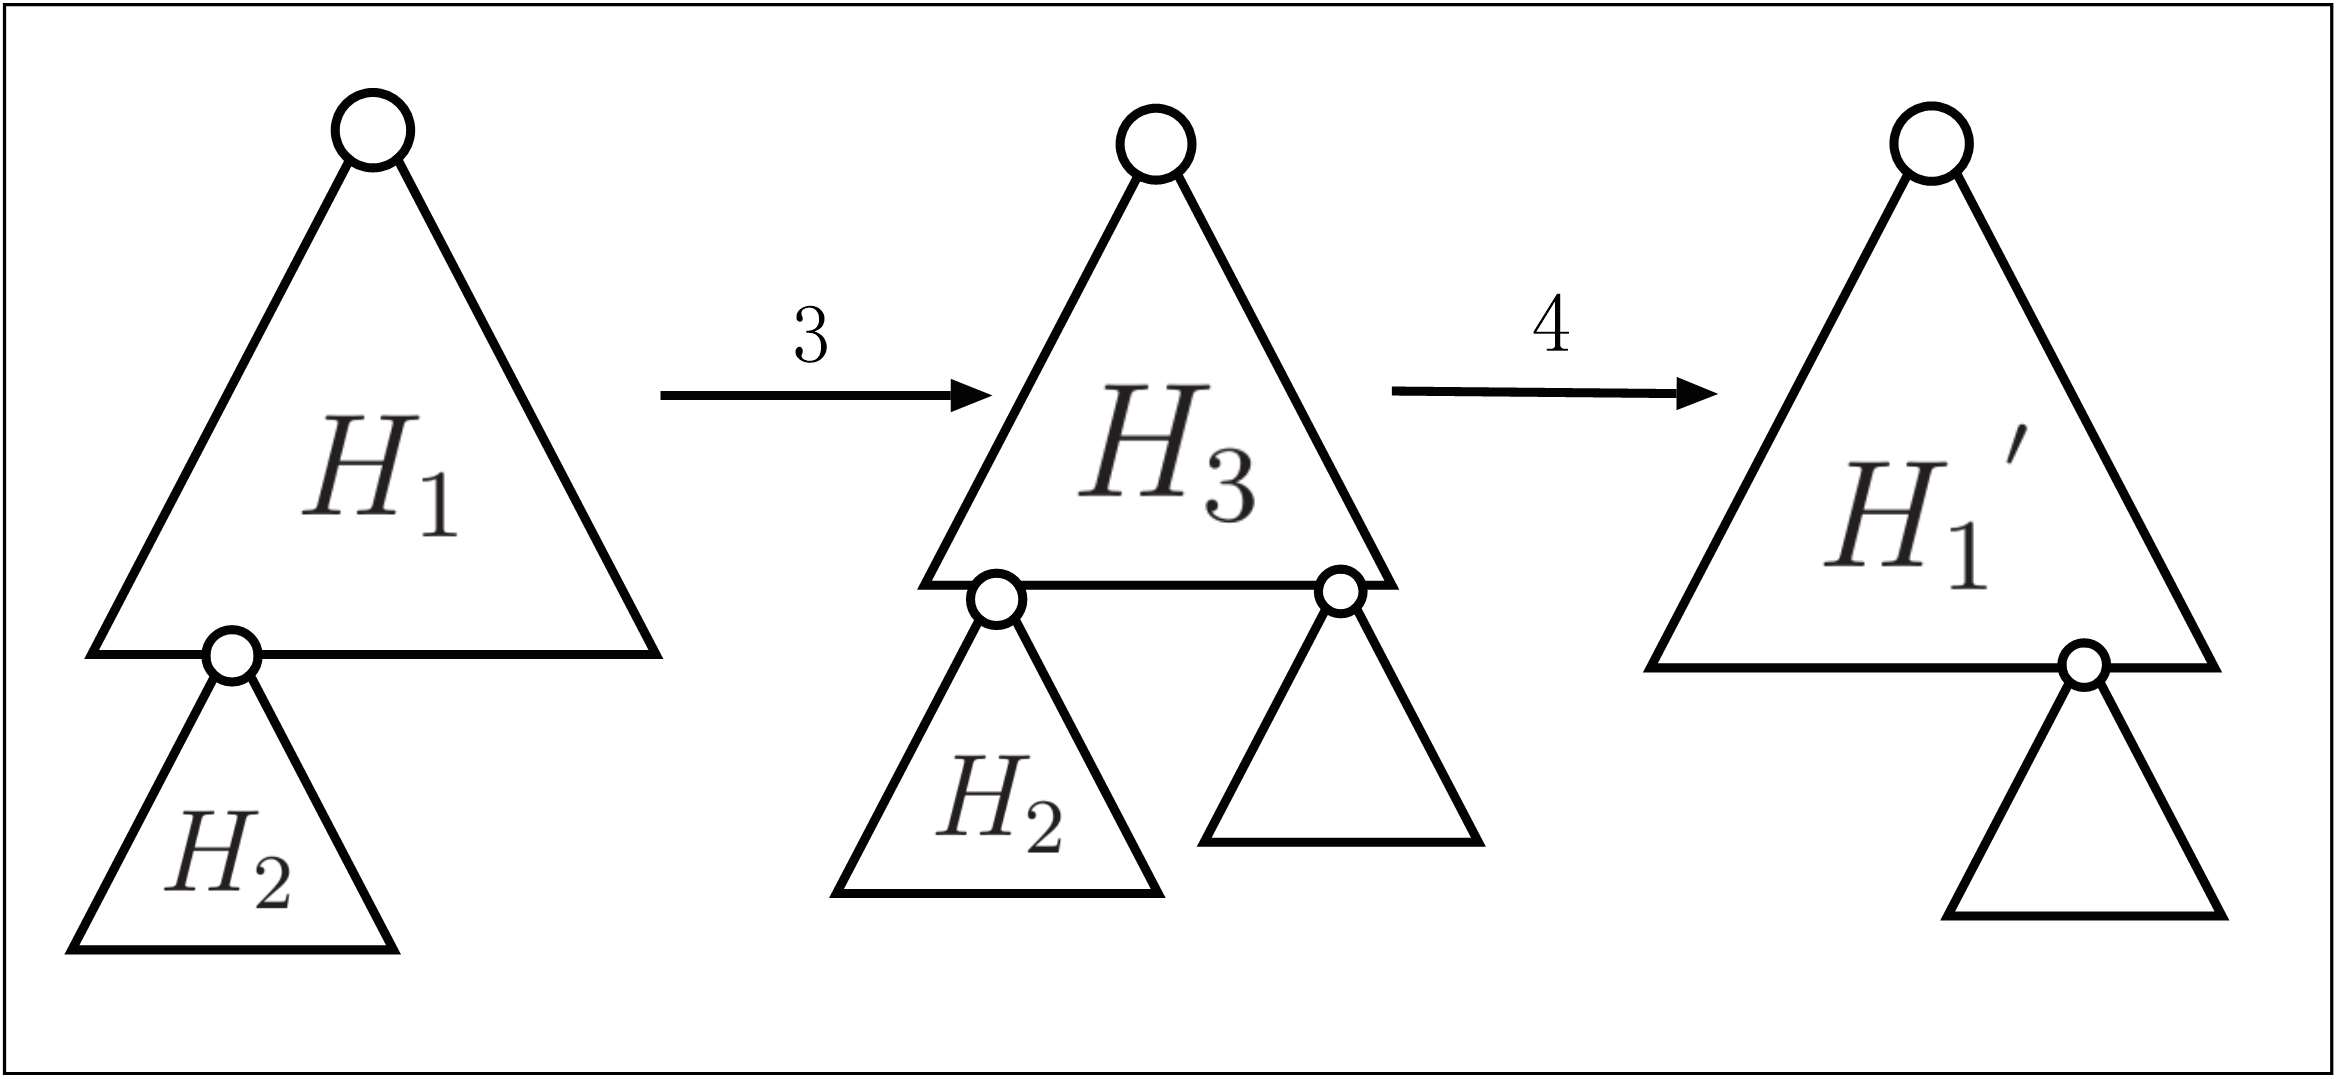
\includegraphics[width=0.8\textwidth]{Medien/Tango/cutJoin}
	\caption{Darstellung von Schritt $3$ und $4$ der \textit{access} Operation. }
	\label{fig:cutJoin}
\end{figure}
Abbildung \ref{fig:cutJoin} zeigt die Schritte $3$ und $4$ des Ablaufes.
Zu klären ist noch, warum im sechsten Punkt die Wurzel des richtigen Hilfsbaumes gefunden werden muss.\\ Seien $u$ und $u_c$ Knoten in $P$, so dass $u_c$ das linke Kind von $u$, aber nicht das preferred child von $u$ ist. Sei $v$, bzw. $v_c$ der Knoten in $T$ mit $\mathit{key}\left(v\right) = \mathit{key}\left(u\right)$, bzw. $\mathit{key}\left(v_c\right) = \mathit{key}\left(u_c\right)$. Sei $H_1$ mit der Wurzel $w_1$ der Hilfsbaum, der $v$ enthält und $H_2$ mit der Wurzel $w_2$ der Hilfsbaum, der $v_c$ enthält. Es muss einen Pfad $P = \left(v_0, v_1,.., v_m \right)$ geben, mit $v_0 = w_1$, $v_m = w_2$ und $v_{m-1}$ ist in $H_1$ enthalten. Aufgrund der Links-Rechts-Beziehung in $H_1$, muss $v_m$ entweder das linke Kind von $v$ sein oder das rechte Kind des Vorgängers $v_v$ von $v$ in $H_1$. \\
Sei $v_m$ das rechte Kind von $v_v$. Dann kann $v$ nicht im rechten Teilbaum von $v_v$ liegen (im linken natürlich auch nicht). Angenommen $v$ ist kein Vorfahre von $v_v$, dann muss es einen Knoten $w$ geben, mit $v_v$ liegt im linken Teilbaum von $w$ und $v$ im rechten Teilbaum. Ein Widerspruch dazu, dass $v_v$ der Vorgänger von $v$ ist.\\
Es gibt also in jedem Fall einen Pfad von $v$ zu $w_2$ in $T$. $w_2$ kann bezogen auf $T$ nur im linken Teilbaum von $v$ enthalten sein. Für alle in $H_1$ enthaltenen Schlüssel $k_1$ gilt entweder $k_1 > \mathit{key}\left(v\right) > \mathit{key}\left(v_v\right) $ oder \\ $ \mathit{key}\left(v\right) > \mathit{key}\left(v_v\right) > k_1 $. Somit muss $w_2$ gefunden werden, indem wie in Schritt sechs vorgegangen wird. 


\subsection{Laufzeitanalyse für access}
Zunächst wird mit zwei Lemmata die Einzeloperation betrachtet, bevor es dann im Satz um Zugriffsfolgen geht. Alle drei Abschnitte basieren auf \cite{demainDinamicOpti}.

 
\begin{Lemma} \label{demaineLemma4}
	Sei $n$ die Anzahl der Knoten eines Tango Baumes $T_{i-1}$. Sei $k$ die Anzahl der Knoten, bei denen sich während der Ausführung von \textit{access}$\left(x_i\right)$ eine Änderung des preferred child ergeben hat. Für die Laufzeit \textit{access}$\left(x_i\right)$ gilt dann $O\left(\left(k + 1\right) \left(1 + \log \left( \log  \left(n \right)\right)\right)\right)$.
\end{Lemma}
\begin{proof}
	Bezeichne $T_i$ den Tango Baum nach der Ausführung von \textit{access}$\left(x_i\right)$. Zuerst werden die Kosten für das Suchen betrachtet. Der Zeiger $p$ der Operationen startet maximal $k + 1$ mal an der Wurzel des Tango Baumes. Für die Länge eines Pfades innerhalb eines Hilfsbaumes gilt $O\left(\log \left( \log  \left(n \right)\right)\right)$, denn für die Anzahl der Knoten eines preferred path gilt $O\left( \log \left(n\right)  \right)$ und ein Hilfsbaum muss ein balancierter BST sein. Die Gesamtkosten ergeben sich damit zu $O\left(\left(k + 1\right) \left(1 + \log \left( \log  \left(n \right)\right)\right)\right)$.\\
	Nun werden die Kosten zum Erzeugen von $T_i$ aus $T_{i-1}$ betrachtet. Pro Veränderung eines preferred child kommt es zu Kosten $O\left(1 + \log\left(\log \left(n\right)\right)\right)$ aufgrund einer \textit{cut} und einer \textit{join} Operation. Für das Suchen des Hilfsbaumes in Punkt $6$ der Beschreibung entstehen auch wieder Kosten von $O\left(\log \left( \log  \left(n \right)\right)\right)$. Somit gilt auch für die Gesamtkosten $O\left(\left(k + 1\right) \left(1 + \log \left( \log  \left(n \right)\right)\right)\right)$.
	
	
\end{proof}
\noindent Sei $\mathit{IB}_i\left(X\right)$ die Differenz von $\mathit{IB}\left(x_1, x_2,..,x_i\right)$ und  $\mathit{IB}\left(x_1, x_2,..,x_{i-1}\right)$. 

\begin{Lemma} \label{demaineLemma5}
	Sei $T$ ein Tango Baum mit dem Referenzbaum $P$. 
	Während der Ausführung von \textit{access}$\left(x_i\right)$ wechselt in $P$ bei genau $\mathit{IB}_i\left(X\right)$ Knoten das preferred child vom linken Kind zum rechten Kind oder vom rechten Kind zum linken Kind.
\end{Lemma}
\begin{proof}
	Sei $p \in P$. Das preferred child von $p$ wechselt während  \textit{access}$\left(x_i\right)$ von links nach rechts,  wenn $x_i$ in der rechten Region von $p$ liegt und der letzte Zugriff innerhalb des Teilbaumes mit der Wurzel $p$ in der linken Region von $p$ lag.  Das preferred child von $p$ wechselt während  \textit{access}$\left(x_i\right)$ von rechts nach links,  wenn $x_i$ in der linken Region von $p$ liegt und der Schlüssel des vorherigen Zugriffs innerhalb des Teilbaumes mit der Wurzel $p$ in der rechten Region von $p$ lag. Das entspricht jeweils genau einem Interleave durch $p$. Zu beachten ist noch, dass der erste Zugriff auf den Teilbaum mit der Wurzel $p$ weder zu einem Interleave, noch zu einem Wechsel eines preferred child von links, bzw. rechts zu rechts, bzw. links führt. 	
\end{proof}

\begin{Satz} \label{demaineSatz2}
	Sei $X = x_1, x_2,.., x_m$ eine Zugriffsfolge und $P$ ein dazu erstellter Referenzbaum. 
	Für die Laufzeit eines mit $P$ erstellten Tango Baumes mit $n$ Knoten zum Ausführen von $X$ gilt $O\left(\left(\mathit{OPT}\left(X\right) + n\right)  + \left(  1 + \log\left(\log \left(n\right)\right)\right)   \right)$.
\end{Satz}
\begin{proof}
	Nach Lemma \ref{demaineLemma5} gibt es nicht mehr als  $\mathit{IB}\left(X\right)$ Wechsel der preferred children von links nach rechts oder umgekehrt. Zudem gibt es maximal $n$ zusätzliche Änderungen bei preferred children. (Erstzugriff in den Teilbaum). Die Gesamtanzahl der Änderungen von preferred children ist somit höchstens $\mathit{IB}\left(X\right) + n$. Mit Lemma \ref{demaineLemma4} ergeben sich Gesamtkosten von\\ $O\left(\left(\mathit{IB}\left(X\right) + n +m \right) \left( 1 + \log \left(\log\left(n\right)\right)\right) \right)$. Mit $\mathit{OPT}\left(X\right) \geq \mathit{IB}\left(X\right) /2 -n $ aus Satz \ref{satzDemaine1} ergibt sich 
	$O\left(\left(\mathit{OPT}\left(X\right) + n +m \right) \left( 1 + \log \left(\log\left(n\right)\right)\right) \right)$.\\ Mit $\mathit{OPT}\left(X\right) \geq m$ ergibt sich dann die Behauptung.
\end{proof}
\noindent Für $m \in \Omega\left(n\right)$ gilt dann auch 
$O\left(	\mathit{OPT}\left(X\right) 	\left( 1 + \log \left(\log \left(n\right)\right)\right)	 \right)$.\\
 Kommt es bei \textit{access}$\left(x\right)$ zu $\Omega\left(\log\left(n\right)\right)$ Wechsel bei preferred children, muss der Hilfsbaum an der Wurzel des Tango Baumes $\Omega\left(\log\left(n\right)\right)$ mal durchsucht werden. Somit hat der Tango Baum die Balanced Property aus \mbox{Abschnitt \ref{upperBounds}} nicht. Damit kann er aufgrund der Implikationen aus Abbildung \ref{fig:upperBounds} auch die anderen Eigenschaften aus diesem Abschnitt nicht haben. Später werden zwei $\log\left(\log\left(n\right)\right)$-competitve BST vorgestellt, welche die Balanced Property erfüllen.      

\subsection{Tango Baum konformes Vereinigen beim Rot-Schwarz-Baum.} \label{vereinigen}
Die Ideen und Angaben zu den Laufzeiten in diesem und dem nächsten Abschnitt stammen aus \cite{conSplit}, von Tarjan.
\begin{figure}[H]
	\centering
	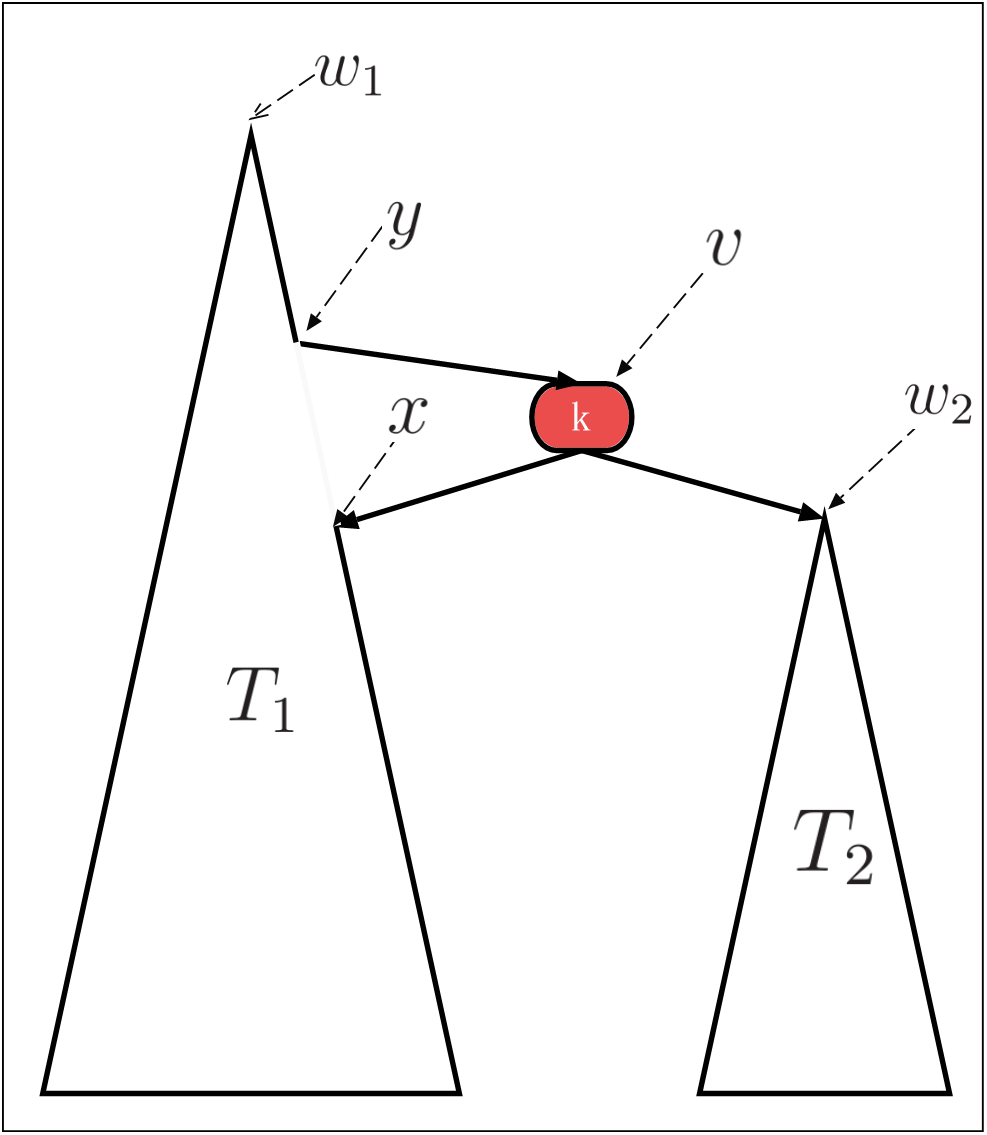
\includegraphics[height= 0.6\textwidth]{Medien/RotSchwarzBaum/vereinigen}
	\caption{Beispielhaftes \textit{concatenate} zweier RBTs unterschiedlicher Schwarz-Höhe, nach Schritt 1. }
	\label{fig:vereinigen}
\end{figure}
\begin{figure}[H]
	\centering
	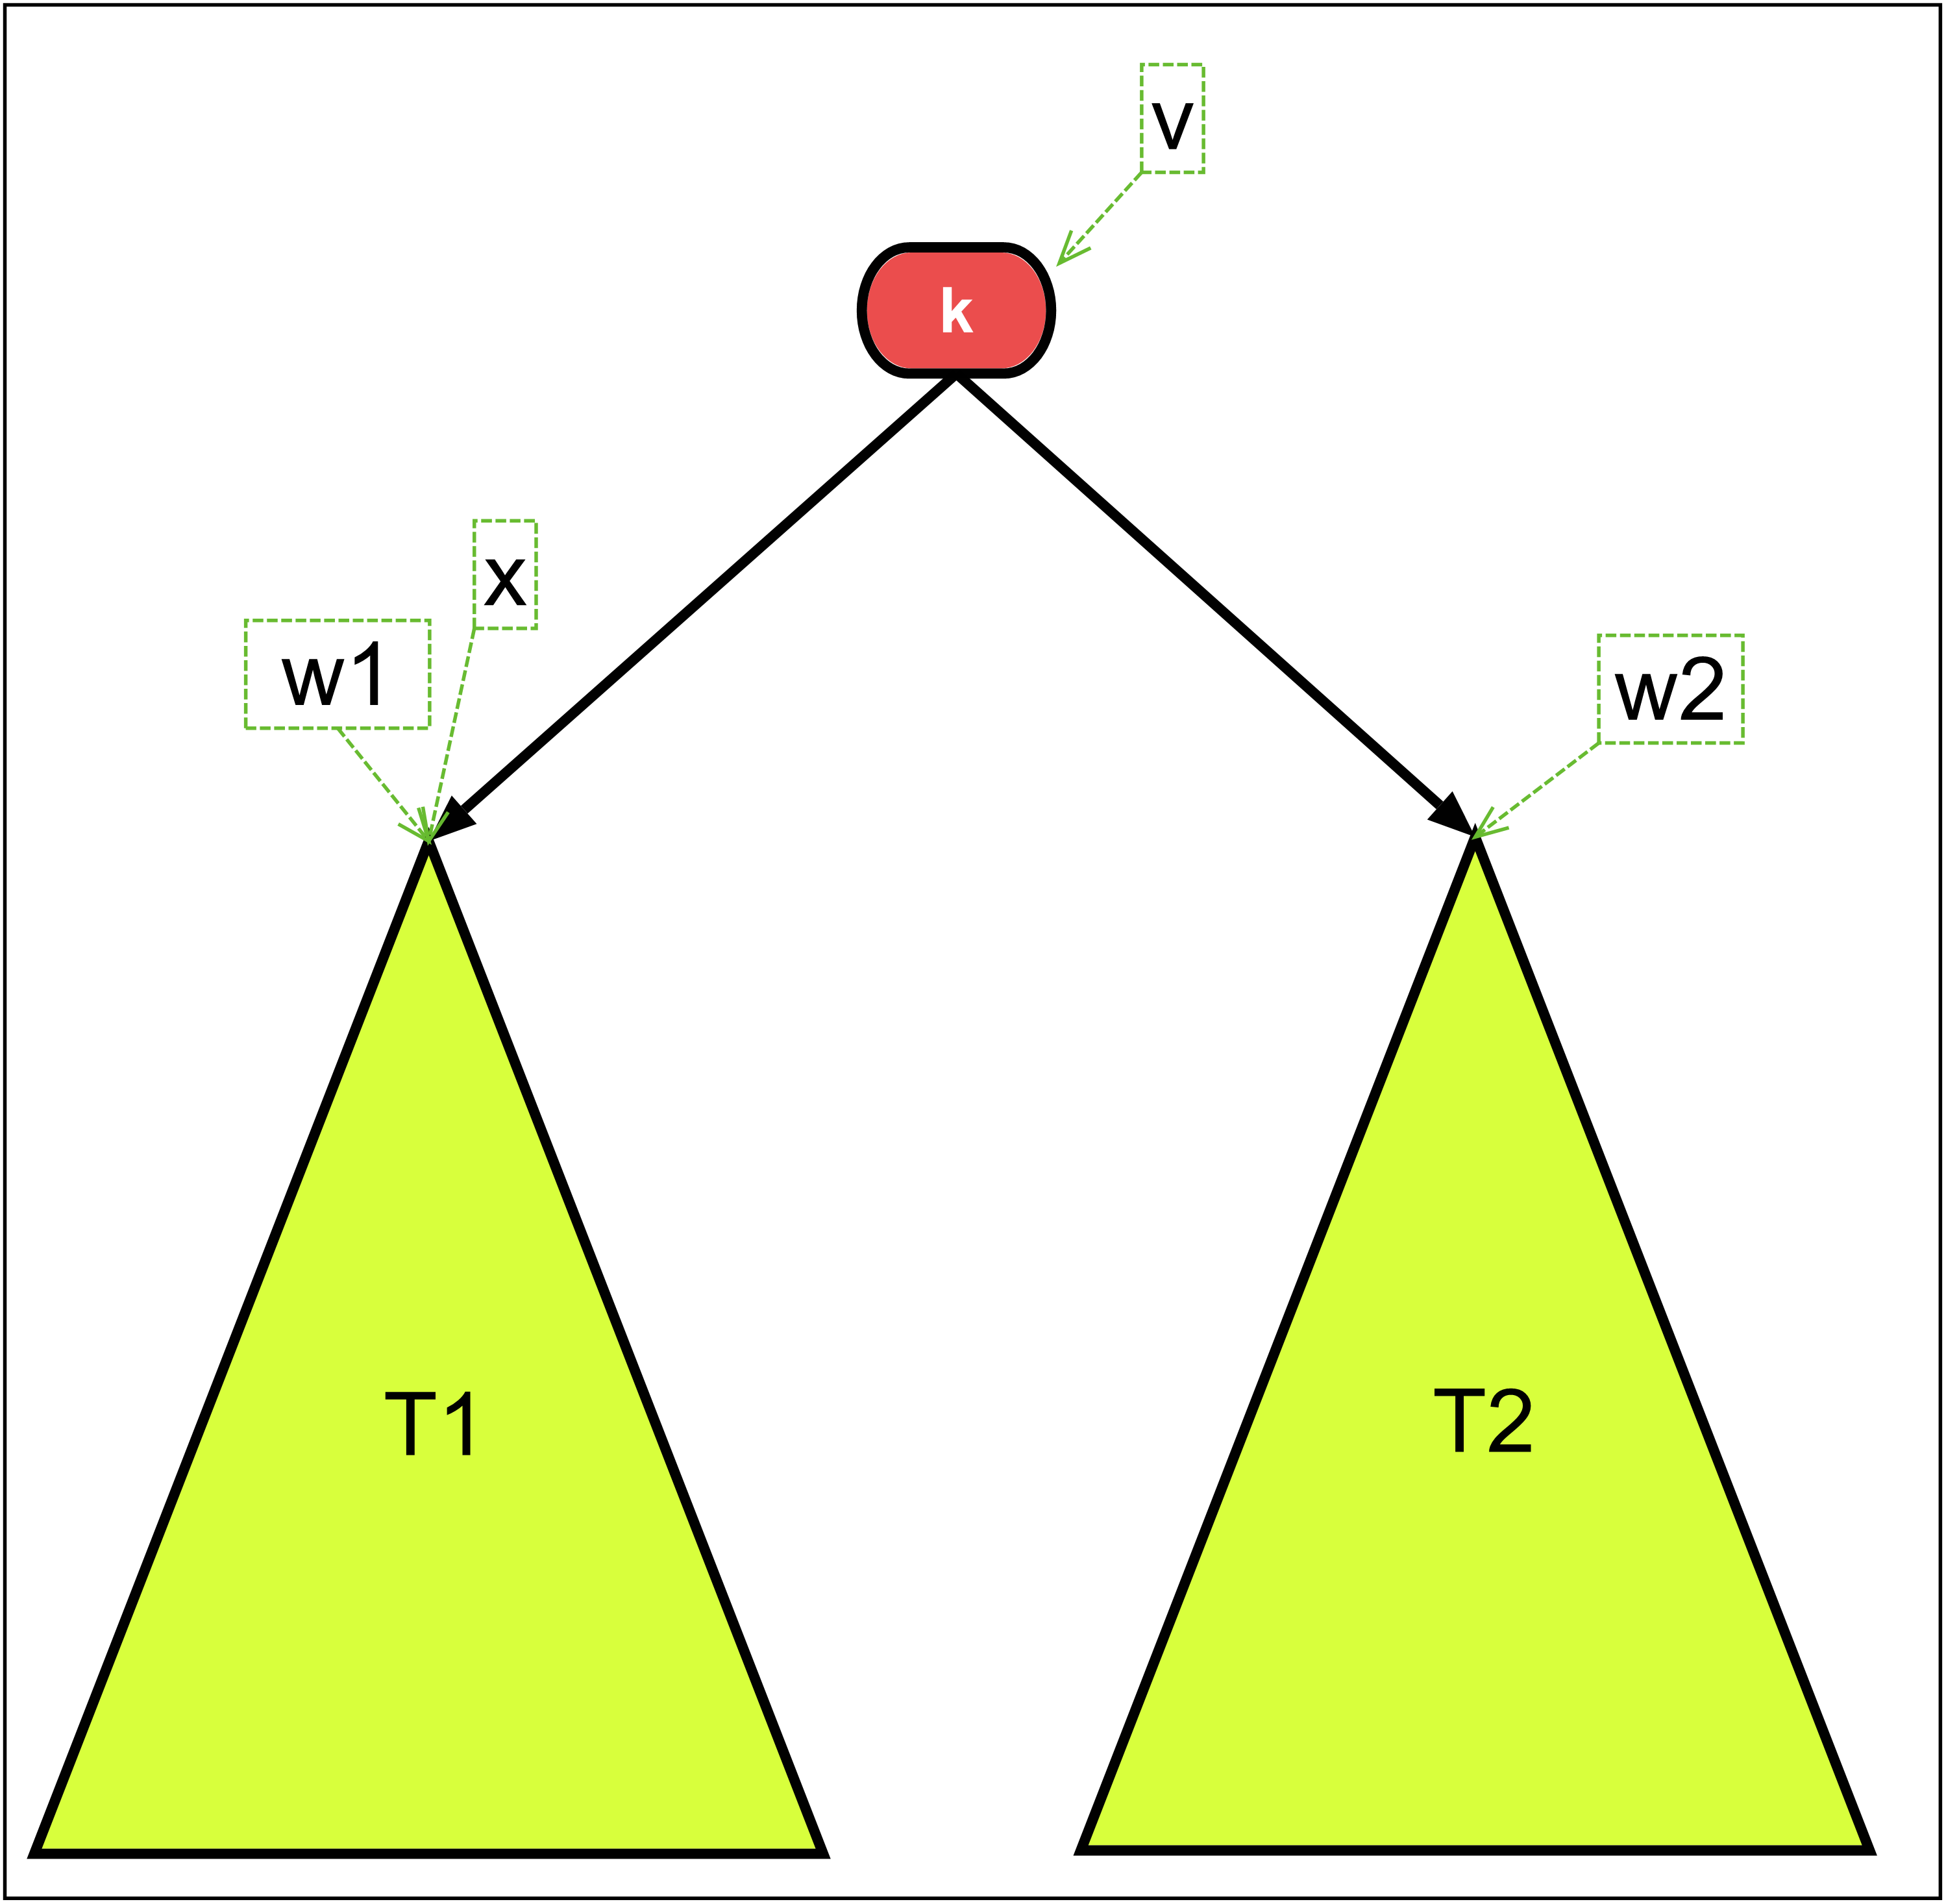
\includegraphics[height= 0.6\textwidth]{Medien/RotSchwarzBaum/vereinigen2}
	\caption{Beispielhaftes \textit{concatenate} zweier RBTs gleicher Schwarz-Höhe, nach Schritt 1. }
	\label{fig:vereinigen2}
\end{figure}
\noindent Hier wird die \textit{concatenate}$($RBT $T_1$, Node $v$, RBT $T_2)$ Operation beim Rot-Schwarz-Baum so eingeführt, wie es für den Tango Baum notwendig ist. Bei der Beschreibung der Operation wird auf die Pflege der Attribute  \textit{minDepth} und \textit{maxDepth} verzichtet, damit sie nicht zu kleinteilig wird. Im Abschnitt zur Laufzeit wird darauf jedoch nochmal eingegangen. Sei $K_1$ die Schlüsselmenge von $T_1$, $K_2$ die Schlüsselmenge von $T_2$ und $k$ der Schlüssel von $v$. Die Operation gibt eine Referenz auf die Wurzel eines vereinigten RBTs $T$ mit der Schlüsselmenge $K_1 \cup K_2 \cup \{k\} $ zurück. Dabei werden $T_1$ und $T_2$ zerstört. An die Parameter wird die Vorbedingung $(\forall i \in K_1: i < k ) \land (\forall j \in K_2: k < j )$ gestellt.\\
Es werden im ersten Schritt der Ausführung drei Fälle unterschieden, wobei wieder der erste zutreffende Fall in aufsteigender Reihenfolge ausgewählt wird. \\
\noindent\textbf{Fall 1: $bh(T_1) = bh(T_2) = 0$ }\\   
In diesem Fall wird die Schwarz-Höhe von $v$  auf $1$ gesetzt, außerdem wird $v$ rot gefärbt. An $v$ werden zwei Sonderknoten angefügt. $v$ ist die Wurzel von $T$. \\
In den restlichen Fällen ist nun immer zumindest ein Baum vorhanden, der über eine Wurzel verfügt. Der RBT mit der kleineren Schwarz-Höhe wird dabei an den mit der größeren \enquote{seitlich angefügt}. Abbildung \ref{fig:vereinigen} zeigt dies beispielhaft. Sind die Schwarz-Höhen gleich, wird wie in Abbildung \ref{fig:vereinigen2} vorgegangen. Nun werden die verbleibenden Fälle beschrieben.\\
\noindent\textbf{Fall 2: $bh(T_2) \leq bh(T_1)$ }\\
In diesem Fall wird $T_2$ bei $T_1$ mit Hilfe von $v$ so angefügt, dass die Schwarz-Höhe jedes Knotens in $T_1$ und $T_2$ unverändert bleibt. Es sei $w_1$ die Wurzel von $T_1$ und $w_2$ die Wurzel von $T_2$. Es sei $P$ ein Pfad $(r_0,r_1,...,r_l)$ in $T_1$, so dass $r_0 = w_1$  gilt, $r_l$ ein Blatt ist und $\forall i \in \{1,2,...l\} \colon r_i$  \textit{ist das rechte Kind von}  $r_{i-1}$ gilt. $P$ ist also der am weitesten rechts liegende Pfad von der Wurzel zu einem Blatt. Sei $x$ der schwarze Knoten in $P$, mit $\mathit{bh}(x) = \mathit{bh}(w_2)$. $x$ muss existieren, denn $\mathit{bh}(w_1) \geq \mathit{bh}(w_2)$ und $\mathit{bh}(r_l) \leq  \mathit{bh}(w_2)$. Außerdem sind $w_1$ und $r_l$ schwarz.\\
Nun wird die Schwarz-Höhe von $v$ auf $\mathit{bh}(x) + 1$ gesetzt. Außerdem wird $v$ rot gefärbt. Als das linke Kind von $v$  wird $x$ gesetzt, als rechtes Kind $w_2$. Ist $x$ die Wurzel von $T_1$, so ist $v$ die Wurzel von $T$. Ansonsten ist $x$ das rechte Kind eines Knotens $y$. Das rechte Kind von $y$ wird auf $v$ gesetzt. Außerdem ist dann $w_1$ die Wurzel von $T$.     \\  
\noindent\textbf{Fall 3: $bh(T_1) < bh(T_2)$ }\\ 
Hier wird $T_1$ bei $T_2$ mit Hilfe von $v$ so angefügt, dass die Schwarz-Höhe jedes Knotens in $T_1$ und $T_2$  unverändert bleibt. Dieser Fall ist fast links-rechts-symmetrisch zu Fall 2. $v$ kann lediglich nicht zur Wurzel von $T$ werden, da $bh(T_1) \neq bh(T_2)$ gilt.

\paragraph{Resultat nach der Fallbehandlung:}
Dass ein Baum mit der Schlüsselmenge  $K_1 \cup K_2 \cup \{k\} $ entstanden ist, ist an den Abbildungen \ref{fig:vereinigen} und \ref{fig:vereinigen2} zu erkennen. Aufgrund der Vorbedingung an die Parameter muss $T$ auch ein BST sein. Es müssen aber wieder die fünf Eigenschaften eines RBTs betrachtet werden:
\begin{enumerate}
	\item Es ist immer noch jeder Knoten entweder rot oder schwarz.
	\item Gilt $bh(T_1) \neq bh(T_2)$, so wurde mit $w_1$ oder $w_2$ ein schwarzer Knoten zur Wurzel von $T$. Anderenfalls ist $v$ die rote Wurzel von $T$ und diese Eigenschaft ist verletzt.   
	\item Aufgrund der Sonderknoten sind die Blätter immer noch schwarz.
	\item Da $T_1$ und $T_2$ RBTs waren muss nur die Situation um $v$ betrachtet werden. $v$ hat in jedem Fall schwarze Kinder. Gilt $bh(T_1) \neq bh(T_2)$ könnte der rote Knoten $v$ jedoch einen roten Elternknoten $y$ haben. 
	\item Die Schwarz-Höhe von $v$ ist korrekt gesetzt. Existiert $y$, so hat sich seine Schwarz-Höhe nicht verändert, da $v$ rot ist. Bei keinem anderen Knoten hat sich bezüglich bzgl. der Schwarz-Höhe etwas geändert. 
\end{enumerate} 
Wir sind also in der Situation, dass nur entweder Eigenschaft zwei oder vier verletzt sein kann. Wenn Eigenschaft vier verletzt ist, dann nur bei Knoten $v$. Das ist genau die Situation, für die \textit{insertFixup} entworfen wurde.\\
In Schritt zwei wird also \textit{insertFixup} mit Parameter $v$ aufgerufen und die Wurzel des resultierenden RBTs zurückgegeben. 
\paragraph{Laufzeit:}
Sei $n_1$ die Anzahl der Knoten von $T_1$, $n_2$ die Anzahl der Knoten von $T_2$ und $n = n_1 + n_2$. Der Tango Baum fordert von seinen Hilfsbäumen eine Laufzeit von $O(\log \left(n\right))$ für die eben vorgestellte Operation.\\ Für die Kosten zum Finden von $x$ und Ausführen von \\ \textit{insertFixup}  gilt $O(\log (n))$. $v$ zu erzeugen und in die Struktur einzubinden benötigt konstante Zeit. 
Die Vorgabe des Tango Baumes wird also eingehalten.\\
Nun wird noch kurz auf die Pflege der Variablen  \textit{minDepth} und \textit{maxDepth} eingegangen. Nach dem ersten Schritt könnten diese Variablen bei allen Knoten im Pfad $P = \left(v_0, v_1, v_m\right)$ mit $v_0$ ist die Wurzel von $T$ und $v_m = v$ falsch gesetzt sein. Um sie zu aktualisieren kann wie folgt vorgegangen werden:\\
 Als erstes wird $v_m$ betrachtet. Es werden die \textit{minDepth} Variablen der Kinder von $v$ und die \textit{depth} Konstante von $v$ betrachtet. $v$.\textit{minDepth} wird auf den kleinsten dieser drei Werte gesetzt. \textit{maxDepth} wird analog aktualisiert. Nun wird mit den restlichen Knoten in $P$ in der Reihenfolge $v_{m-1}, v_{m-2},..,v_0$ genauso vorgegangen. Die Kosten für das Aktualisieren eines Knotens sind konstant und Kosten von $O\left(m\right)$ sind bereits bei der Suche nach $x$ entstanden. \\   
Für den nächsten Abschnitt wird noch eine genauere Betrachtung der Gesamtlaufzeit benötigt:\\ Es sei $d = \vert \mathit{bh}(T_1) - \mathit{bh}(T_2)  \vert $. Die Suche nach $x$ endet spätestens nachdem ein Pfad der Länge $2d + 1$ betrachtet wurde. Dabei steht die $1$ für den Zugriff auf $x$ selbst. Zu jedem schwarzen Knoten könnte noch ein roter Knoten dazukommen, bis $x$ erreicht ist.\\
 Jetzt wird noch auf die maximale Anzahl der Iterationen innerhalb \\ \textit{insertFixup} eingegangen.
 Sei $w$ die Wurzel des vereinigten BSTs nach \mbox{Schritt 1}. $v$ ist ein roter Knoten mit $\mathit{bh}(w) - \mathit{bh}(v) = d - 1$ und befindet sich in der Baumstruktur nicht tiefer als Ebene $2d + 2$. Deshalb führt \textit{insertFixup} maximal $d + 1$ Iterationen durch.  

\subsection{Tango Baum konformes Aufteilen beim Rot-Schwarz-Baum.}
Auch \textit{split} $($RBT $T$, key $k)$ wird so vorgestellt, wie es für den Tango Baum notwendig ist. Vorbedingung an die Parameter ist, dass $k$ in der Schlüsselmenge $K$ von $T$ vorhanden ist. Zurückgegeben wird eine Referenz auf den Knoten ${v_k}'$ mit dem Schlüssel $k$. Das linke Kind von ${v_k}'$ ist die Wurzel eines RBTs $T_L$ mit der Schlüsselmenge $K_L$, wobei gilt ${K_L=\{i \mid  i\in K \land i <k\}}$. Das rechte Kind von ${v_k}'$ ist die Wurzel eines RBTs $T_R$ mit der Schlüsselmenge $K_R$, wobei gilt ${K_R = \{i \mid i\in K \land i > k\}}$. \textit{split} gibt also in den meisten Fällen nicht die Wurzel eines RBTs zurück.\\ Die Operation setzt zunächst $T_L$ auf den linken Teilbaum von $v_k$ und $T_R$ auf den rechten Teilbaum von $v_k$. Eventuell müssen die Wurzeln von $T_R$ und $T_L$ schwarz gefärbt werden. Sei $(v_0,v_1,..,v_m)$  der Pfad von der Wurzel von $T$ zu $v_k$. Es wird sich nun bei $v_{m-1}$ startend, Knoten für Knoten in dem Pfad nach oben gearbeitet. Ist der Schlüssel eines Knotens kleiner als $k$, so wird dieser Knoten und der linke Teilbaum des Knotens zu $T_L$ hinzugefügt. Dies übernimmt die \textit{concatenate} Operation. Ist der Schlüssel größer als $k$, so wird der Knoten und dessen rechter Teilbaum  zu $T_R$ hinzugefügt. Folgende Aufzählung beschreibt den Vorgang genauer:

\begin{enumerate}
	\item Verwende die \textit{search} Operation, um den Knoten $v_k$ mit dem Schlüssel $k$ zu finden.
	\item Setze den linken Teilbaum von $v_k$ als $T_L$, den rechten als $T_R$. Löse beide Teilbäume aus $T$ heraus.
	\item Färbe die Wurzeln von $T_L$ und $T_R$ schwarz.
	\item $\forall i \in \{0,1,..,m-1\}$ absteigend sortiert. Ist der Schlüssel $k_i$ von $v_i$ kleiner als $k$, vereinige $T_L$ mit dem aus $T$ herausgelösten linken Teilbaum von $v_i$, mit  $v_i$ als dritten Parameter. Ansonsten vereinige $T_R$ mit dem aus $T$ herausgelösten rechten Teilbaum von $v_i$ mit  $v_i$ als dritten Parameter. Färbe die Wurzel des herausgelösten Teilbaumes vor dem Vereinigen schwarz. 
	\item Füge $T_R$ rechts an $v$ an, $T_L$ links.
	\item Gib ${v_k}'$ zurück.
\end{enumerate}   
Das $T_L$ und $T_R$ die gewünschten RBTs sind wird leicht erkannt. $v_0$ und einer seiner beiden Teilbäume wird korrekt zugeordnet. Die Wurzel des anderen Teilbaumes von $v_0$ ist $v_{1}$. Alle Schlüssel, die nicht im Teilbaum mit der Wurzel $v_{1}$ liegen sind somit korrekt zugeordnet. Diese Betrachtung iteriert bis auf $v_k$ getroffen wird. Die Schlüssel im Teilbaum mit der Wurzel $v_k$ werden korrekt zugeordnet. 

\paragraph{Laufzeit:}
Der Tango Baum fordert eine Laufzeit von $O(\log(n))$ von seinen Hilfsbäumen für \textit{split}, mit $n$ ist die Anzahl der Knoten. Punkt 1 kostet $O(\log(n))$. Durchführen von Punkt 2, 3, 5 und 6 kostet $O(1)$. Punkt 4 führt $O(\log (n))$ Aufrufe von \textit{concatenate} durch. Das ergibt $O(\log (n) \log (n))$, was dann auch eine obere Schranke für die Gesamtlaufzeit darstellt. Diese Schranke ist für unseren Einsatzzweck jedoch zu hoch.\\ Deshalb wird Punkt 4 nun genauer betrachtet, speziell die Konstruktion von $T_L$. Es sei $l$ die Anzahl der Aufrufe von \textit{concatenate} nach denen $T_L$ neu gesetzt wird. Sei $\{t_1,t_2,..,t_l\}$ die Menge der aus $T$ herausgelösten Teilbäume, die für die $l$ Aufrufe verwendet werden, wobei $t_1$ zum ersten Aufruf gehört, $t_2$ zum zweiten, usw.. $T_0$ steht für den linken Teilbaum von $v_k$.  Sei $i \in \{1, 2, .., l\}$. $T_i$ ist der Zustand von $T_L$, nachdem \textit{concatenate} mit Parameter $t_i$ ausgeführt wurde. $v_i$ ist der Elternknoten der Wurzel von $t_i$.\\

\noindent
Es gilt $\mathit{bh} \left(t_i \right) \leq \mathit{bh} \left(v_{i} \right)$ und $\mathit{bh} \left(t_i \right) < \mathit{bh} \left(v_{i+1} \right)$.\\
Nun wird durch Induktion über $i$ gezeigt, dass eine der beiden folgenden Aussagen immer gelten muss:\\
\bigskip
\begin{enumerate}
	\item  $\mathit{bh} \left(T_{i} \right) \leq  \mathit{bh} \left(v_{i+1} \right)$
	\item $\mathit{bh} \left(T_{i} \right) =  \mathit{bh} \left(v_{i+1} \right) +1$, beide Kinder der Wurzel von $T_i$ sind schwarz und $\mathit{bh} \left(v_{i} \right) = \mathit{bh} \left(v_{i+1} \right)$
\end{enumerate}
 
\noindent Für $i = 0$ gilt $T_i$ ist der linke Teilbaum von $v_k$ und $\mathit{bh} \left(v_{1} \right) > \mathit{bh} \left(T_{i} \right)$.\\
Induktionsschritt:\\
$T_i =$ \textit{concatenate}$\left(T_{i-1}, v_i, t_i\right)$.\\

\noindent \textbf{Für $T_{i-1}$ gilt Aussage 1:}\\
Es gilt entweder $\mathit{bh} \left(T_{i} \right) = \max\{\mathit{bh} \left(T_{i-1}\right), \mathit{bh} \left(t_{i} \right) \} $  oder \\ $\mathit{bh} \left(T_{i} \right) = \max\{\mathit{bh} \left(T_{i-1}\right), \mathit{bh} \left(t_{i} \right) \} + 1$. Ist das Erstere der Fall, ist nichts mehr zu zeigen. Beim anderen Fall galt entweder  $\mathit{bh} \left(T_{i-1} \right) =  \mathit{bh} \left(t_{i} \right)$ oder \\ \textit{insertFixup} hat die Schwarz-Höhe der Wurzel um eins erhöht. In beiden Fällen hat die Wurzel von $T_i$ zwei schwarze Kinder, vergleiche Abschnitt \ref{if2}. Gilt  $\mathit{bh} \left(v_{i} \right) < \mathit{bh} \left(v_{i+1} \right)$, ist Aussage eins korrekt, ansonsten Aussage zwei.\\

\noindent \textbf{Für $T_{i-1}$ gilt Aussage 2:}\\
 Es gilt $\mathit{bh} \left(T_{i} \right) = \mathit{bh} \left(T_{i-1} \right)$, denn $\mathit{bh} \left(T_{i-1} \right) > \mathit{bh} \left(t_{i} \right)$ und \textit{insertFixup} kann die Schwarz-Höhe eines RBTs  ohne rotes Kind der Wurzel nicht erhöhen, vergleiche Abschnitt \ref{if2}. Sollte $v_i$ durch den ersten Schritt der Operation zu einem roten Kind der Wurzel geworden sein, so hat $v_i$ beim Aufruf von \textit{insertFixup} einen schwarzen Elternknoten. Auch in diesem Fall erhöht \mbox{\textit{insertFixup}} die Schwarz-Höhe des Baumes nicht. Mit  $\mathit{bh} \left(v_{i-1} \right) = \mathit{bh} \left(v_{i} \right)$ muss  $\mathit{bh} \left(v_{i} \right) < \mathit{bh} \left(v_{i+1} \right)$ gelten. Somit ist für $T_i$ die Aussage eins korrekt.\\

 

\noindent Für $\mathit{bh} \left(t_{i} \right) < \mathit{bh} \left(T_{i-1} \right)$ folgt daher  $\vert\mathit{bh} \left(t_{i} \right) -\mathit{bh} \left(T_{i-1} \right) \vert = O\left(1\right) $ \\ und daraus
\begin{align*}
\sum_{i = 1}^{l} \vert\mathit{bh} \left(t_{i} \right) -\mathit{bh} \left(T_{i-1} \right) \vert =  O \left(\log \left(n \right) \right) 
\end{align*}


\noindent Der Gesamtaufwand für das Suchen von $v$ in allen $l$ Aufrufen berechnet sich mit: 
\begin{align*}
\sum_{i = 1}^{l}  2 \vert\mathit{bh}(t_{i}) -\mathit{bh}(T_{i-1}) \vert + 1 =
2 \left( \sum_{i = 1}^{l}   \vert\mathit{bh}(t_{i}) -\mathit{bh}(T_{i-1}) \vert \right)+ l
= O \left(\log \left(n \right) \right)
\end{align*}
\noindent Für die Anzahl der Iterationen von \textit{insertFixup} in allen $l$ Aufrufen gilt: 
\begin{align*}
\sum_{i = 1}^{l}   \vert\mathit{bh}(t_{i}) -\mathit{bh}(T_{i-1}) \vert +1 =
\sum_{i = 1}^{l}  \left( \vert\mathit{bh}(t_{i}) -\mathit{bh}(T_{i-1}) \vert \right) + l 
= O \left(\log \left(n \right) \right)
\end{align*}
Die Kosten innerhalb einer Iteration sind konstant. Damit ist  $O \left(\log \left(n \right) \right)$ eine obere Schranke für die Gesamtkosten zum Konstruieren von $T_L$. Für $T_R$ gilt analog das Gleiche. Für die Gesamtkosten von \textit{concatenate} innerhalb \textit{split} gilt $O \left(\log \left(n \right) \right)$, denn die Kosten für das Suchen und \textit{insertFixup} überlagern die restlichen Kosten. Damit ist $O \left(\log \left(n \right) \right)$ eine obere Schranke für die Kosten von Punkt 4 und somit auch für \textit{split}. Der hier vorgestellte RBT hält also die Anforderung des Tango Baumes bezüglich der Laufzeit von \textit{split} ein.


\begin{figure}[H]
	\centering
	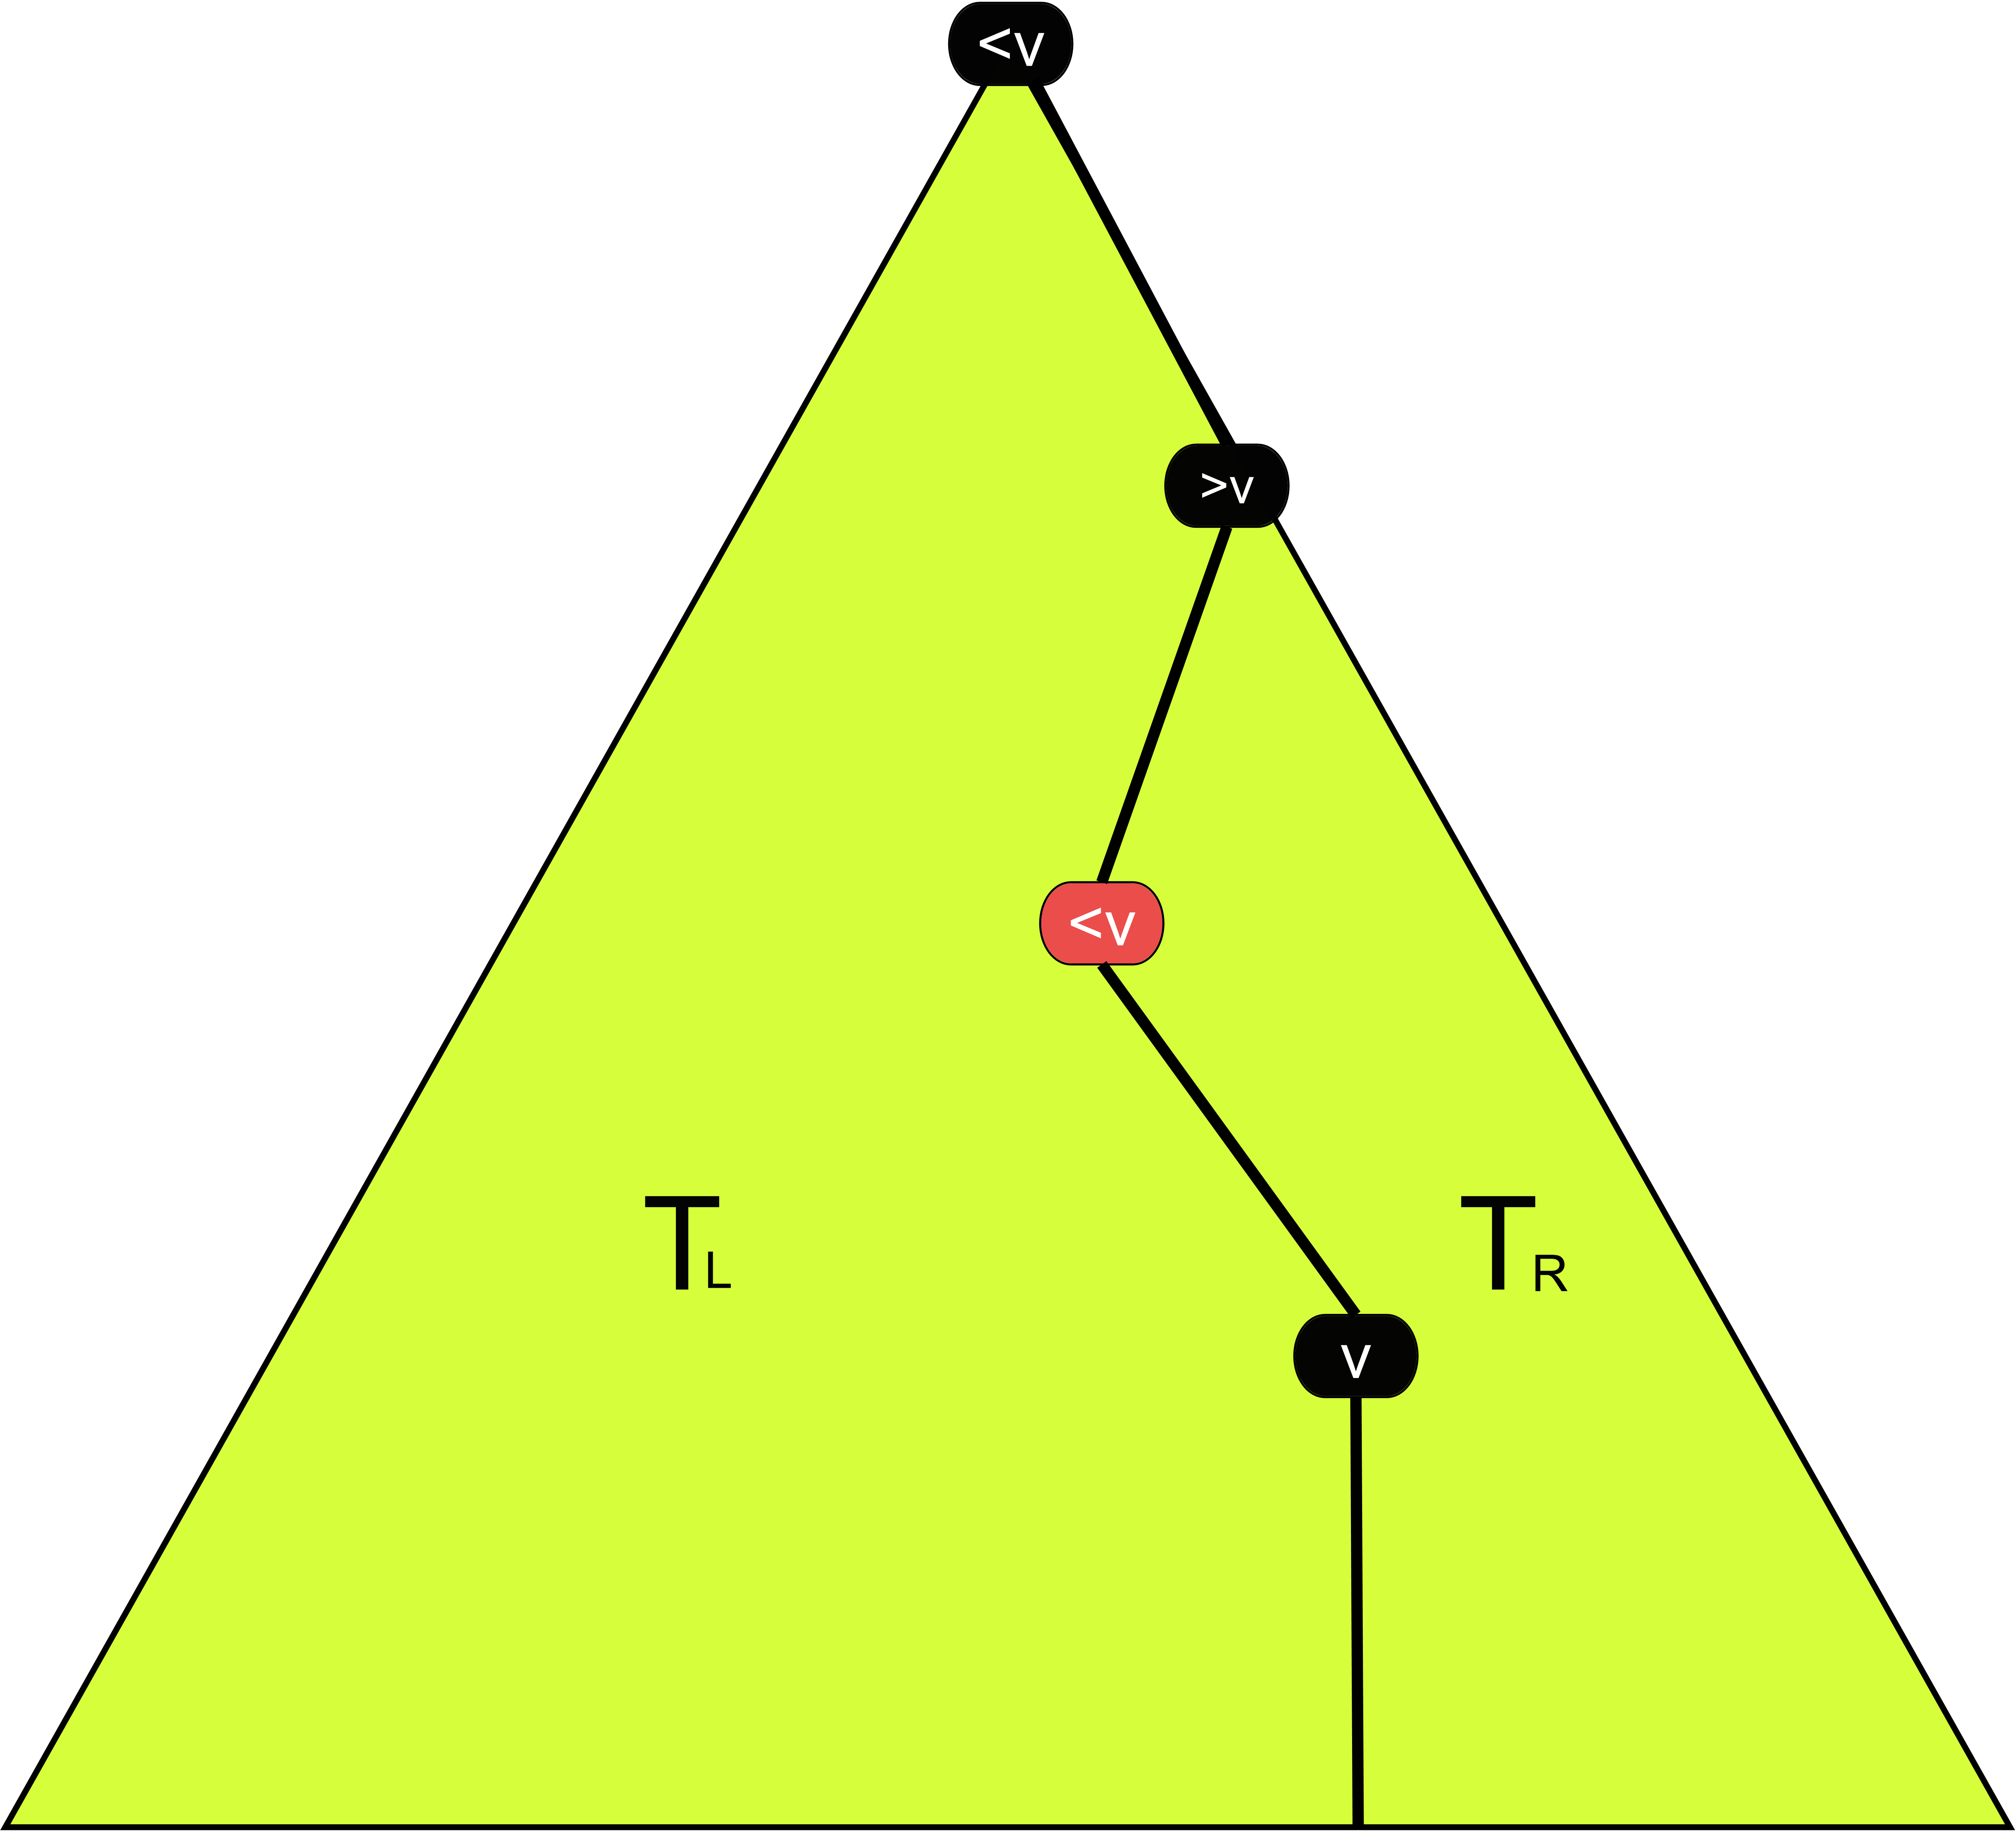
\includegraphics[width=0.8\textwidth]{Medien/RotSchwarzBaum/aufteilen}
	\caption{Beispielhaftes \textit{split} eines RBTs mit Parameter $v$. Die Symbole in den Knoten beziehen sich auf die Schlüssel der Knoten. }
	\label{fig:aufteilen}
\end{figure}


\section{Splay Baum}
Der  Splay Baum \cite{splay} ist ein dynamischer BST, der ohne zusätzliche Hilfsdaten in seinen Knoten auskommt. Nach einer \textit{access}$\left(k\right)$ Operation ist der Knoten mit dem Schlüssel $k$ die Wurzel des Splay Baumes. Es gibt keine Invariante, welche eine bestimmte maximale Höhe garantiert. Splay Bäume können sogar zu Listen entarten. Amortisiert betrachtet verfügen sie dennoch über sehr gute Laufzeiteigenschaften. 


\subsection{Die \textit{access} Operation beim Splay Baum. }
Die wesentliche Arbeit leistet eine Hilfsoperation namens \textit{splay}$($key $k)$. Nach deren Ausführung befindet sich der Knoten mit dem gesuchten Schlüssel $k$ an der Wurzel und es wird nur noch eine Referenz auf ihn zurückgegeben.

\paragraph{\textit{splay} Operation:}
Sei $p$ der Zeiger der Operation in den BST. Zunächst wird eine gewöhnliche Suche ausgeführt, bis $p$ auf den Knoten $v$ mit dem Schlüssel $k$ zeigt. Nun werden iterativ sechs Fälle unterschieden, bis $v$ die Wurzel des Baumes darstellt. Zu jedem Fall gibt es einen der links-rechts-symmetrisch ist. Sei $u$ der Elternknoten von $v$. 

\begin{enumerate}
	\item $v$ ist das linke Kind der Wurzel (zig-Fall):\\
	Es wird eine Rechtsrotation auf $v$ ausgeführt. Nach dieser ist $v$ die Wurzel des Splay Baumes und die Operation wird beendet. 
	\item $v$ ist das rechte Kind der Wurzel (zag-Fall):\\
	Symmetrischer Fall zu zig.
	\item $v$ ist ein linkes Kind und $u$ ist ein linkes Kind (zig-zig-Fall):\\
	Dieser Fall unterscheidet den Splay Baum von einem anderen BST (move-to-root) mit schlechteren Laufzeiteigenschaften. Es wird zuerst eine Rechtsrotation auf $u$ ausgeführt und erst danach eine Rechtsrotation auf $v$. Bei move-to-root  ist es genau umgekehrt. 
	\item $v$ ist ein rechtes Kind und $u$ ist ein rechtes Kind. (zag-zag-Fall):\\
	Symmetrischer Fall zu zig-zig.
	\item $v$ ist ein linkes Kind und $u$ ist ein rechtes Kind (zig-zag-Fall):\\
	Es wird eine Rechtsrotation auf $v$ ausgeführt. Im Anschluss wird eine Linksrotation auf $u$ ausgeführt.
	\item $v$ ist ein rechtes Kind und $u$ ist ein linkes Kind (zag-zig-Fall):\\
	Symmetrischer Fall zu zig-zag.
	
\end{enumerate}
Abbildung  \ref{fig:zigZag} zeigt drei der Fälle. Trotz der Einfachheit kann die Auswirkung einer einzelnen \textit{splay} Operation groß sein. Abbildung \ref{fig:splay} \cite{splay} zeigt eine solche Konstellation. \\
Die Laufzeit von \textit{access} auf einem Splay Baum mit $n$ Knoten ist $O\left(n\right)$.

\begin{figure}[H]
	\centering
	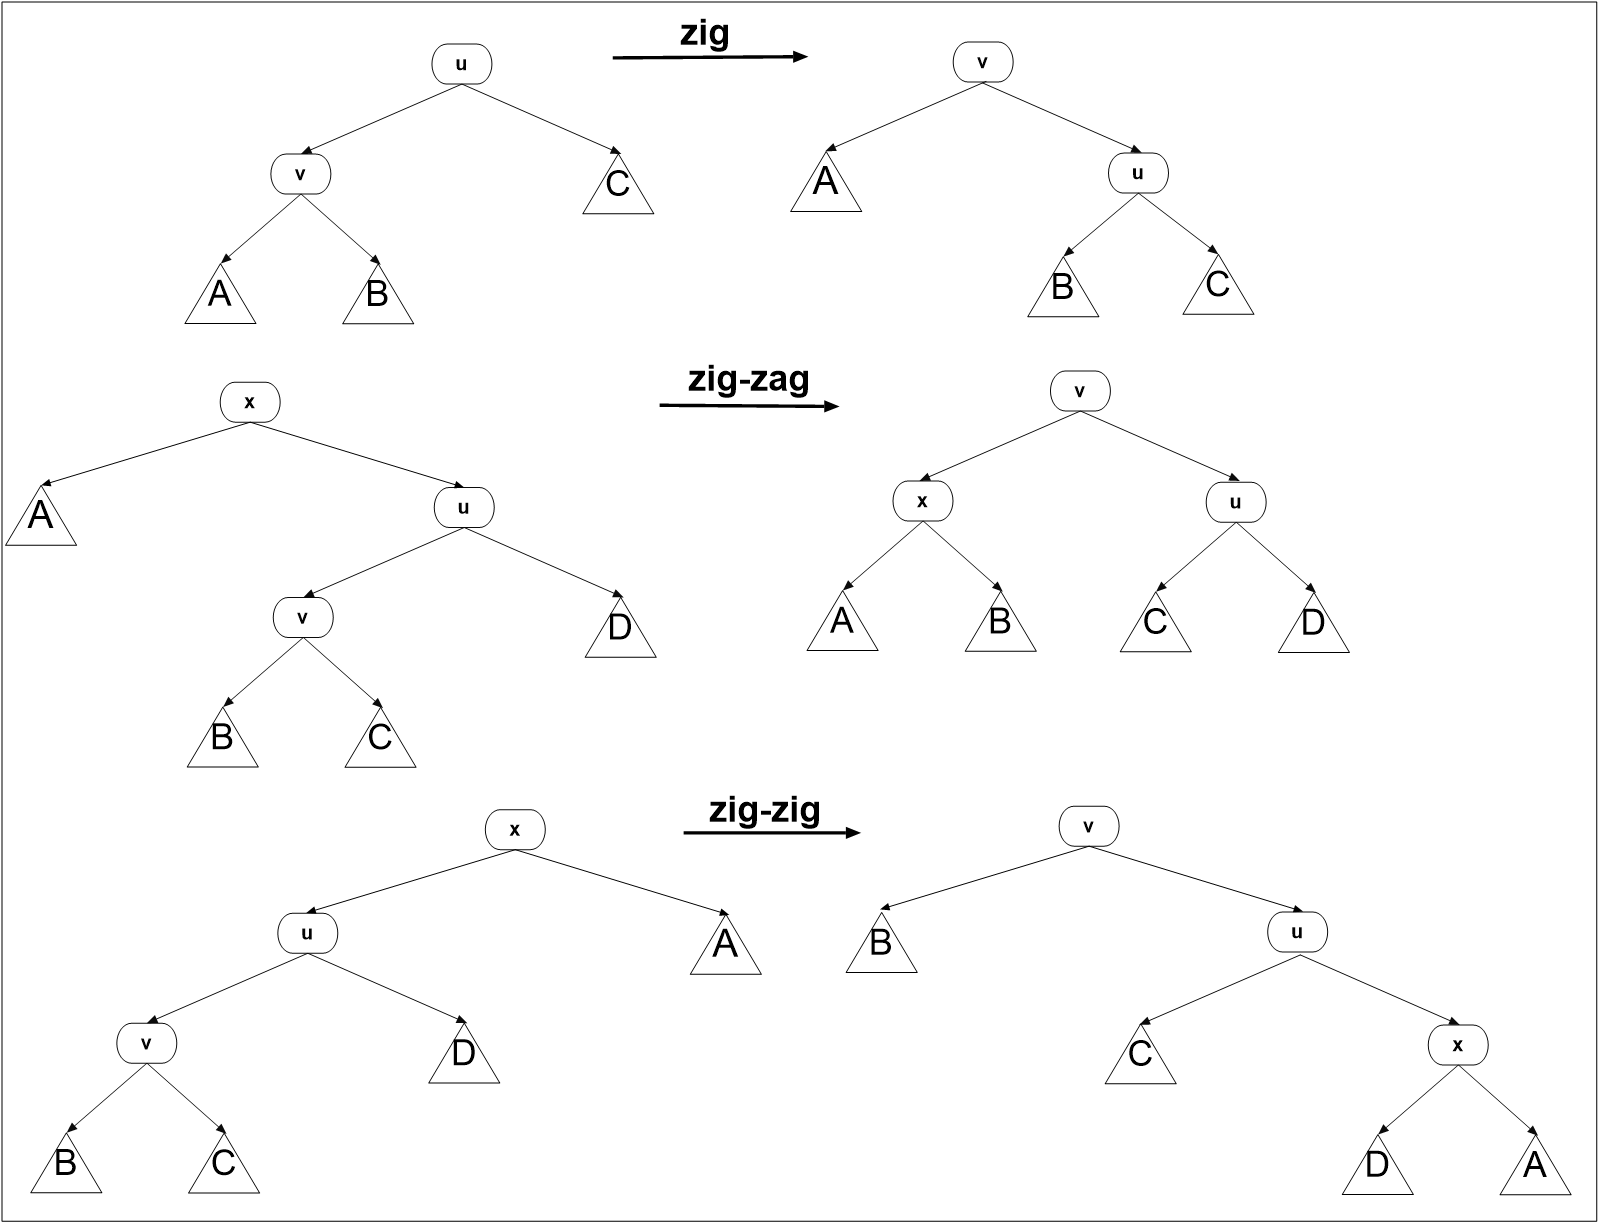
\includegraphics[width= 1.2\textwidth]{Medien/Splaybaum/zigZag}
	\caption{Darstellung von zig, zig-zig und zig-zag. }
	\label{fig:zigZag}
\end{figure}
\begin{figure}[H]
	\centering
	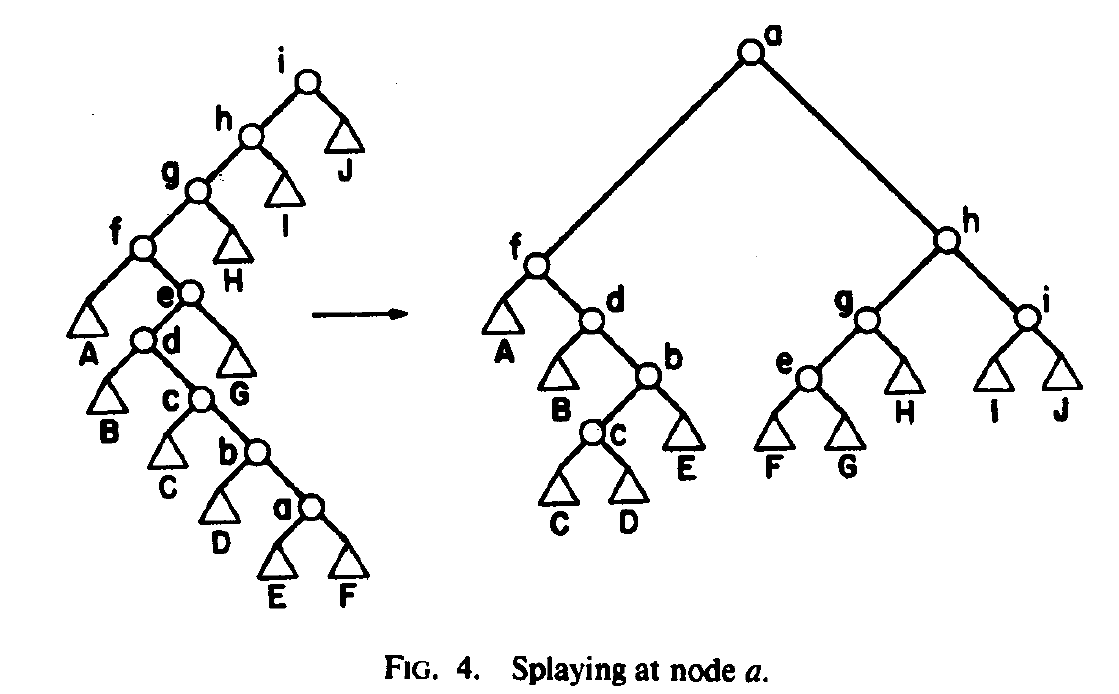
\includegraphics[width= 1\textwidth]{Medien/Splaybaum/splay}
	\caption{Eine einzige \textit{splay } Operation.\cite{splay}}
	\label{fig:splay}
\end{figure}

\subsection{Amortisierte Laufzeitanalyse von \textit{splay}.}
Es wird die Potentialfunktionsmethode aus Kapitel \ref{potentialfunktionsmethode} verwendet. Sei $v$ ein Knoten im Splay Baum $T$. Eine Funktion $w\left(v\right)$ liefert zu jedem Knoten eine reelle Zahl $>0$, die \textbf{Gewicht} genannt wird. Eine Funktion $\mathit{tw}\left(v\right)$ bestimmt die Summe der Gewichte aller im Teilbaum mit der Wurzel $v$ enthaltenen Knoten. Der \textbf{Rang}  $r\left(v\right)$ ist definiert durch $r\left(v\right) = \log_2 \left( \mathit{tw}\left(v\right)\right)$. Sei $V$ die Menge der Knoten von $T$. Als Potentialfunktion wird 
\begin{align*}
\Phi = \sum_{v \in V} r\left(v\right)
\end{align*}
verwendet.





\newtheorem{Lemma1}{Access Lemma}[section] \label{lemmaSplay}
\begin{Lemma1}Sei $T$ ein Splay Baum mit $n$ Knoten, Wurzel $w$ und einem Knoten $v$ mit dem Schlüssel $k$. Die amortisierte Laufzeit von \textit{splay}$\left(k\right)$ ist maximal $3 \left(r\left(w\right) - r\left(v\right)\right) + 1 = O\left(\log\left(\mathit{tw}\left(w\right) / \mathit{tw}\left(v\right)\right) \right) = O\left(\log\left(n\right)\right)$. \\
	
\end{Lemma1}
\begin{proof}
	Es werden den Knoten fest zugeordnete Gewichte angenommen. Zunächst wird für \textit{zig}, \textit{zig-zig} und \textit{zig-zag} gezeigt, dass die amortisierten Kosten nicht größer als $3 \left(r\left(v\right)' - r\left(v\right)\right) + 1$ sind. Für die anderen drei Fälle folgt es dann aus der Symmetrie. Im Anschluss wird die gesamte Operation  betrachtet. An Abbildung  \ref{fig:zigZag} ist zu erkennen, dass sich der Wert von $\mathit{tw}\left(\right)$ nur an den Knoten $v$, dessen Elternknoten $u$  und dem Elternknoten $x$ von $u$ verändern kann.  Damit gilt:
	\begin{align*}
	\Phi' - \Phi  = r\left(u\right)' +r\left(v\right)' +r\left(x\right)' - r\left(u\right)- r\left(v\right)- r\left(x\right)
	\end{align*}
	
	
	\paragraph{zig:} 
	In diesem Fall existiert $x$ nicht, damit gilt:\\  {$ \Phi' - \Phi  = r\left(u\right)' +r\left(v\right)' - r\left(u\right)- r\left(v\right)$}. Der Wert von $\mathit{tw}\left(\right)$ für die Wurzel ist unabhängig vom Zustand des Splay Baumes, da an ihr alle im Baum vorhandenen Gewichte summiert werden. Deshalb muss  $\mathit{tw}\left(v\right)' =  \mathit{tw}\left(u\right)$ gelten. Daraus folgt $ \Phi' - \Phi  = r\left(u\right)'- r\left(v\right)$. Aus $r\left(v\right)' \geq r\left(u\right)'$ folgt \\ $ \Phi' - \Phi \leq  r\left(v\right)'- r\left(v\right) \leq 3\left(r\left(v\right)'- r\left(v\right)\right) $. Addieren von $1$ aufgrund der Rotation ergibt Kosten $\leq 3\left(r\left(v\right)'- r\left(v\right)\right) + 1$.
	\paragraph{zig-zig:} 
	Es müssen zwei Rotationen ausgeführt werden. Deshalb entstehen amortisierte Kosten von
	\begin{align*}
	&2 + r\left(u\right)' +r\left(v\right)' +r\left(x\right)' - r\left(u\right)- r\left(v\right)- r\left(x\right) \textit{ ,mit $r\left(x\right) =  r\left(v\right)'$ }\\
	=& 2 + r\left(u\right)' +r\left(x\right)' - r\left(u\right)- r\left(v\right) \textit{,mit
		$r\left(v\right)' \geq  r\left(u\right)' \land r\left(u\right) \geq  r\left(v\right)$}\\
	\leq &  2 + r\left(v\right)' + r\left(x\right)' - 2 r\left(v\right) 
	\end{align*}
	Nun wird zunächst die Behauptung aufgestellt, dass dieser Ausdruck klein genug ist. Dies wird dann über Äquivalenzen gezeigt:
	\begin{align*}
	& 2 + r\left(v\right)' + r\left(x\right)' - 2 r\left(v\right) \leq  3\left(r\left(v\right)'- r\left(v\right)\right)\\
	\Leftrightarrow &2 \leq 2r\left(v\right)' -  r\left(x\right)' - r\left(v\right)\\
	\Leftrightarrow & -2 \geq -2r\left(v\right)' +  r\left(x\right)' + r\left(v\right)\\
	\Leftrightarrow & -2 \geq \log_2\left(\mathit{tw}\left(x'\right) / \mathit{tw}\left(v'\right)\right) + \log_2\left(\mathit{tw}\left(v\right) / \mathit{tw}\left(v'\right)\right)
	\end{align*}
	Dass die letzte Ungleichung gilt, kann an einer Eigenschaft des $\log_2$ abgeleitet werden. Für $a,b \in \mathit{R}$ mit $a,b > 0$ und $a + b \leq 1$ gilt $\log_2\left(a\right) + \log_2\left(b\right) \leq -2$. An Abbildung \ref{fig:zigZag} ist zu erkennen, dass sich $\mathit{tw}\left(v\right)$ vom Ausgangszustand zum gestrichelt dargestellten Zwischenschritt hin nicht verändert. $\mathit{tw}\left(x'\right)$ ist ebenfalls unverändert zum Zwischenschritt. Es kann also bei beiden Knoten mit den Werten aus dem Zwischenschritt gearbeitet werden. Bezeichne $u^*$ den Knoten $u$ im Zwischenschritt, dann gilt $ \mathit{tw}\left(u^*\right) = \mathit{tw}\left(v'\right)$. \\  Daraus folgt $\mathit{tw}\left(v'\right) = \mathit{tw}\left(x'\right) + \mathit{tw}\left(v\right) + w\left(u\right) $ und daraus \\ \mbox{$\left(\mathit{tw}\left(x'\right) + \mathit{tw}\left(v\right)\right) /  \mathit{tw}\left(v'\right) < 1$} und mit der Eigenschaft von $\log_2$ folgen die Ungleichungen.
	
	\paragraph{zig-zag:} 
	\begin{align*}
	&2 + r\left(u\right)' +r\left(v\right)' +r\left(x\right)' - r\left(u\right)- r\left(v\right)- r\left(x\right) \textit{ ,mit $r\left(x\right) =  r\left(v\right)' \land r\left(v\right) \leq  r\left(u\right)$} \\
	\leq& 2 + r\left(u\right)' +r\left(x\right)' - 2 r\left(v\right)
	\end{align*}
	Nun wird wie bei zig-zig vorgegangen:
	\begin{align*}
	&  2 + r\left(u\right)' +r\left(x\right)' - 2 r\left(v\right) \leq  2\left(r\left(v\right)'- r\left(v\right)\right)\\
	\Leftrightarrow &2 \leq 2r\left(v\right)' -  r\left(x\right)' - r\left(u\right)'\\
	\Leftrightarrow &-2 \geq -2\left(v\right)' +  r\left(x\right)' + r\left(u\right)'\\
	\Leftrightarrow & -2 \geq \log_2\left(\mathit{tw}\left(x'\right) / \mathit{tw}\left(v'\right)\right) + \log_2\left(\mathit{tw}\left(u'\right) / \mathit{tw}\left(v'\right)\right)
	\end{align*}
	Mit der $\log_2$ Regel aus zig-zig und Abbildung \ref{fig:zigZag} folgt die Behauptung, wobei diesmal lediglich der Endzustand betrachtet werden muss.
	Zum Berechnen der Kosten der Gesamtoperation werden die Kosten der einzelnen Fallbehandlungen summiert. Dabei bildet sich eine Teleskopsumme, die möglicherweise, wenn ein  zig, bzw. zag Fall enthalten ist, mit eins addiert werden muss. Daraus folgt das Lemma.
\end{proof}

\subsection{Dynamische Optimalitäts Vermutung}
Der Splay Baum erfüllt die Working Set Property und die Dynamic Finger Property aus Abschnitt \ref{upperBounds} und auch noch viele weitere in dieser Arbeit nicht aufgeführte Eigenschaften. Der Beweis zur Dynamic Finger Property ist sehr aufwändig \cite{dynFinger}. Dass der Splay Baum die Working Set Property besitzt, wurde bereits bei seiner Vorstellung gezeigt\cite{splay}. Dieser Beweis wird hier vorgestellt. Die anderen Eigenschaften (außer dynamisch optimal) aus Kapitel \ref{upperBounds} folgen dann aus diesen beiden. Aufgrund dieser oberen Schranken der Laufzeit des Splay Baumes wurde die Vermutung aufgestellt, dass der Splay Baum dynamisch optimal ist. Bewiesen ist bisher nur, dass er $\log \left(n\right)$-competitive ist. Dies folgt aus dem Access Lemma. Würde für eine solche obere Schranke gezeigt werden, dass der Splay Baum diese nicht einhalten kann, jedoch ein anderer BST schon, wäre die Vermutung zur dynamischen Optimalität widerlegt. Auch das ist bis heute nicht geschehen. \\

\noindent Wiederholung der Definition von $a_i$ zu einer Zugriffsfolge $X = x_1, x_2,.., x_m$ aus Kapitel \ref{upperBounds}:\\
Für $x_i$ sei $J_i = \{j \in \mathbb{N} \vert j < i \land x_j = x_i \}$.
Sei $t_{xi} = \max \left(J_i\right)$, falls $J_i$ nicht leer ist, ansonsten $t_{xi} = 0$. $t_{xi}$ liefert also den Index des vorherigen Zugriffes auf $x_i$, falls ein solcher existiert. Sei ${a_i = \vert\{x_j \vert t_{xi} < j \leq i   \} \vert }$.

\newtheorem{Satz2}{Working Set Property}[section] \label{workingSetSplay}
\begin{Satz2} Es sei $T$ ein Splay Baum mit $n$ Knoten. Sei $X = x_1,x_2,..,x_m$ eine für $T$ erstellte Zugriffsfolge. Dann gilt für die amortisierte Laufzeit zum Ausführen von $X$: \\
	$O\left( n \log\left(n\right) + m +\sum_{i = 1}^{m} \log\left( a_i\right) \right)$.
\end{Satz2}
\begin{proof}
	Den Knoten werden die Gewichte $1, 1/2^2,1/3^2 .., 1/n^2$ zugeordnet. Diesmal ist die Zuordnung nicht fest. Nach jeder \textit{access} Operation können sich Gewichte ändern. Sei $i$ der kleinste Index mit $x_i = \mathit{key}\left(v\right)$ für einen Knoten $v$. Sei $b = \vert\{x_l \vert l < i\}\vert$, dann wird $v$ zum Start das Gewicht $1 / 2^{b+1}$ zugeordnet. Auf Knoten, auf deren Schlüssel nicht zugegriffen wird, verteilen sich die kleinsten Gewichte beliebig. $\mathit{tw}\left(v\right)$ und $\Phi$ sind definiert wie beim Access Lemma.\\
	Nach einer \textit{access} $\left(x_j\right)$ Operation werden die Gewichte neu zugeordnet. Der Knoten $v_j$ mit dem Schlüssel $x_j$ erhält das Gewicht $1/1$. Sei $1/k^2$ das Gewicht von $v_j$ vor \textit{access} $\left(x_j\right)$. Sei $u$ ein Knoten mit $w\left(u\right) = 1 / k^*$ mit \\ $k^* \in \{1, 4,.., \left(k-1\right)^2\}$ direkt vor \textit{access} $\left(x_j\right)$. Dann ist $1 /\left(k^* + 1\right)^2$ das Gewicht von $u$ nach \textit{access} $\left(x_j\right)$. Die Gewichte der restlichen Knoten bleiben unverändert. Zu beachten ist, dass nach einer solchen Neuzuordnung die Menge der im Baum enthaltenen Gewichte unverändert bleibt. \\
	Diese Verteilung der Gewichte garantiert, dass direkt vor  \textit{access} $\left(x_j\right)$, $v_j$ ein Gewicht von ${1 /a_i}^2$ hat, somit gilt $\mathit{tw}\left(v_j\right) \geq {1 /a_i}^2$ . Der Wert von $\mathit{tw}\left(\right)$ für die Wurzel von $T$ ist $W = \sum_{i = 1}^{n} 1/ n^2 < 2 = O\left(1\right) $. Diese Werte in das Access Lemma eingesetzt, ergibt Kosten von \\ $O\left(\log\left(1 / \left({1 /a_i}^2\right)\right)\right) = O\left(\log\left({a_i}^2 \right)\right) = O\left(log\left(a_i\right)\right)$.\\
	 Durch die nachfolgende Neuzuordnung der Gewichte kann $\Phi$ nur kleinere Werte annehmen. Denn nur das Gewicht der neuen Wurzel erhöht sich. $\mathit{tw}\left(\right)$ ist für die Wurzel aber konstant.\\
	Der Rang eines Knotens kann über die gesamte Zugriffsfolge nicht um mehr als $\log_2\left(n^2 W\right) = O\left(log\left(n\right)\right)$ kleiner werden. Denn $W$ ist der maximale Wert von $\mathit{tw}\left(\right)$ und  der minimale ist $1 /n^2$. Daraus folgt eine maximale Verringerung des Potentials von $T$ von $O\left(n \log \left(n\right)\right)$. 
\end{proof}



\section {Weitere dynamische Suchbäume}
Hier werden kurz zwei Variationen zum Tango Baum vorgestellt. Zum einen der Zipper Baum \cite{zipper}. Er ist ebenfalls $\log\left(\log\left(n\right)\right)$-competitive,  garantiert aber auch  $O\left(\log \left(n\right)\right)$ im worst case, bei einer einzelnen \textit{access} Operation. $n$ steht wieder für die Anzahl der Knoten. Zum anderen der Multisplay Baum \cite{multisplay}. Bei diesem wird ein preferred path durch einen Splay Baum repräsentiert. Amortisiert betrachtet erreicht er $O\left(\log \left(n\right)\right)$ bei \textit{access} und ist  $\log\left(\log\left(n\right)\right)$-competitive. 

\subsection{Zipper Baum}
Der Zipper Baum basiert auf dem Tango Baum und nutzt auch preferred paths aus einem Referenzbaum $P$. Aufbau und Pflege der preferred paths in $P$ unterscheiden sich nicht zu denen beim Tango Baum.  Ihre Repräsentation im eigentlichen BST $T$ macht den wesentlichen Unterschied zu einem Tango Baum aus. Abbildung \ref{fig:zipperPathRep} stellt eine solche beispielhaft dar.  Sei $v$ ein Knoten in $T$, dann ist in diesem Kapitel $v^*$ der Knoten in $P$ mit $\mathit{key}\left(v\right) =\mathit{key}\left(v^*\right)$. Die Repräsentation eines preferred path  $P_p = \left({p_1}^*,{p_2}^*,..,{p_m}^*\right)$ in $T$ stellt einen Hilfsbaum $H$ dar, der in zwei Teile unterteilt ist, dem \textbf{zipper} und dem \textbf{bottom tree}.  Der bottom tree ist ein balancierter BST, der genau die Schlüssel enthält, die in $P_p$ enthalten sind, jedoch nicht im zipper. Der zipper besteht aus zwei Teilen, dem \textbf{top zipper} $z_t$ und dem \textbf{bottom zipper} $z_b$. $z_t$ und $z_b$ dürfen jeweils maximal $\log_2\left(\log_2\left(n\right)\right)$ Knoten enthalten. Gemeinsam  enthalten sie zumindest $\log_2\left(\log_2\left(n\right)\right) / 2$ Knoten, wenn ein bottom tree existiert. Bei weniger als $\log_2\left(\log_2\left(n\right)\right) / 2$ Knoten im Hilfsbaum existiert kein bottom tree. Es wird im Folgenden angenommen, dass ein bottom tree existiert. \\
$P_p$ wird in \textbf{zig Segmente} und \textbf{zag Segmente} unterteilt. Ein zig Segment in $P_p$ ist ein längst möglicher Pfad in $P$, indem nur Knoten aus $P_p$ enthalten sein dürfen, deren rechtes Kind ebenfalls in $P_p$ enthalten ist. zag Segmente werden analog gebildet, wobei das linke Kind ebenfalls in $P_p$ enthalten sein muss, anstatt dem rechten. Dazu gibt es noch die Ausnahme, dass der Knoten mit der größten Tiefe in $P_p$ dem Segment seines Elternknotens zugeordnet wird.\\
Sei $S_{zig}$ die Folge der in zig Segmenten enthaltenen Knoten, aufsteigend sortiert nach der Tiefe und $S_{zag}$ die Folge der in zag Segmenten enthalten Knoten, aufsteigend sortiert nach der Tiefe.  Sei $n_t$, bzw. $n_b$ die Anzahl der Knoten von $z_t$, bzw. $z_b$. $z_t$ repräsentiert Knoten  $P_t = \left({p_1}^*,{p_2}^*,..,p_{n_t}^*\right)$ und $z_b$ die Knoten  $P_b = \left({p_{n_t + 1}}^*,{p_{n_t + 2}}^*,..,{p_{n_t + n_b}}^*\right)$.
Sei ${t_l}^*$ der Knoten der größten Tiefe, der sowohl in $P_t$, als auch in $S_{zig}$ enthalten ist. Sei ${t_r}^*$ der Knoten mit der größten Tiefe, der sowohl in $P_b$, als auch in $S_{zag}$ enthalten ist. $t_l$ ist die Wurzel von $H$. $t_r$ ist das rechte Kind von $t_l$. Der linke Teilbaum von $t_l$  hat Listenform und  enthält die  Knoten, deren Schlüssel auch in  $S_{zig}$ enthalten ist, so dass kein Knoten in diesem Teilbaum ein linkes Kind hat. Der rechte Teilbaum von $t_r$  hat Listenform und  enthält die  Knoten, deren Schlüssel auch in $S_{zag}$ enthalten ist, so dass kein Knoten in diesem Teilbaum ein rechtes Kind hat. \\
$z_b$ wird analog aus $P_b$ erzeugt und seien $b_l$ und $b_r$ die Knoten in $z_b$ entsprechend zu $t_l$ und $t_r$ in $z_t$. $b_l$ ist das linke Kind von $t_r$. Die Wurzel des bottom Tree ist das linke Kind von $b_r$. Dass die Links-Rechts-Beziehung eingehalten wird ergibt sich aus dem Aufbau der zig und zag Segmente. Es ist leicht zu erkennen, dass die Wurzel des bottom tree in konstanter Zeit erreicht werden kann.
\begin{figure}[H]
	\centering
	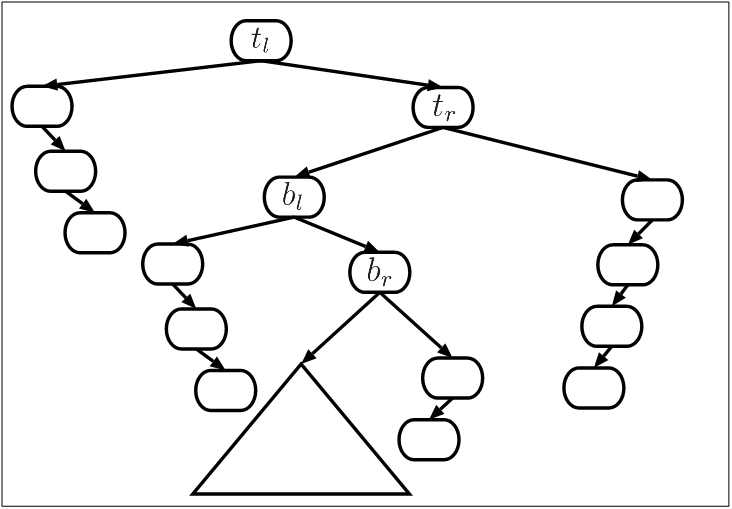
\includegraphics[width= 0.8\textwidth]{Medien/Zipper/zipperPathRep}
	\caption{Pfadrepräsentation beim Zipper Baum, basiert auf einer Abbildung aus \cite{zipper}. }
	\label{fig:zipperPathRep}
\end{figure}
\begin{figure}[H]
	\centering
	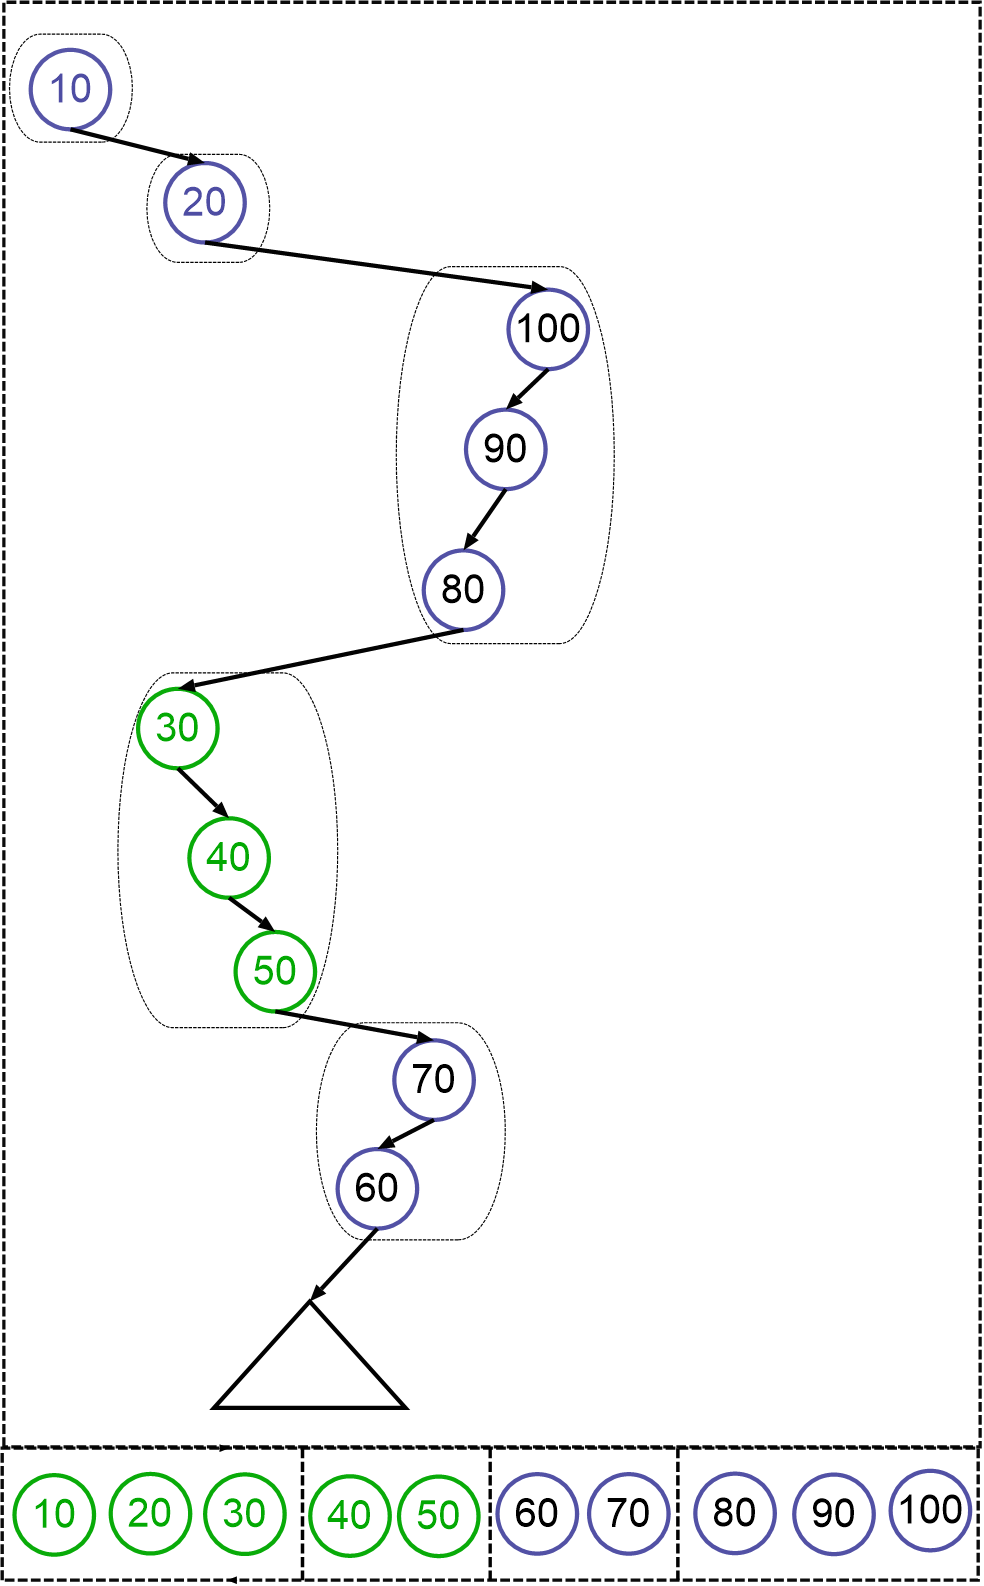
\includegraphics[height= 0.7\textwidth]{Medien/Zipper/preferredPathZigZag}
	\caption{zig Segmente sind grün dargestellt. zag Segmente blau. }
	\label{fig:preferredPathZigZag}
\end{figure}

\paragraph{Besonderheiten bei \textit{access}:}
Sei $l$ die Anzahl der Knoten des top zipper.
Beim Suchen nach einem Schlüssel in einem Hilfsbaum $H$ wird dessen top zipper soweit wie notwendig in einen Pfad gewandelt, der $\left(p_1, p_2, .., p_l\right)$ entspricht. Ist der top zipper vollständig in einen Pfad umgewandelt, wird der Vorgang beim bottom zipper fortgesetzt. Dieser hat dann die Stellung des top zipper. Außerdem wird dann ein \textbf{Extraktionsprozess} angestoßen, der $\log\left(\log\left(n\right)\right)$ Knoten aus dem bottom tree auslagert, um einen neuen bottom zipper zu erzeugen. Für dessen Laufzeit ist entscheidend, dass die Wurzel des bottom tree in konstanter Zeit erreicht werden kann. Ein Extraktionsprozess ist in Abbildung \ref{fig:extractHybrid} dargestellt. $l'$ ist der größte Schlüssel, der kleiner ist, als die Schlüssel der zu extrahierenden Knoten. $r'$ ist entsprechend der kleinste Schlüssel, der größer ist, als diese Schlüssel.  \\
Der nächste Knoten aus dem zipper kann dem Pfad in konstanter Zeit hinzugefügt werden. Ist der gesuchte Knoten $p_v$  im zipper enthalten, entstehen um ${p_v}^*$ in  $P$ zu erreichen, asymptotisch betrachtet die gleichen Kosten, wie in $H$. Ist in $H$ der zipper aufgebracht, sind bereits Kosten von $O\left(\log\left(\log\left(n\right)\right)\right)$ entstanden. Befindet sich der gesuchte Knoten im  bottom tree entstehen in $H$ ebenfalls Kosten von  $O\left(\log\left(\log\left(n\right)\right)\right)$. Diese müssen auch in $P$ entstehen, da dann $v > \log_2\left(\log_2\left(n\right)\right) /2$  gelten muss. Deshalb entstehen asymptotisch betrachtet in $H$ und innerhalb $P$ die gleichen Kosten. In $P$ ist jeder Knoten in $O\left(\log\left(n\right)\right)$ Zeit erreichbar, deshalb ist dies auch für  $T$ der Fall. 


\begin{figure}[H]
	\centering
	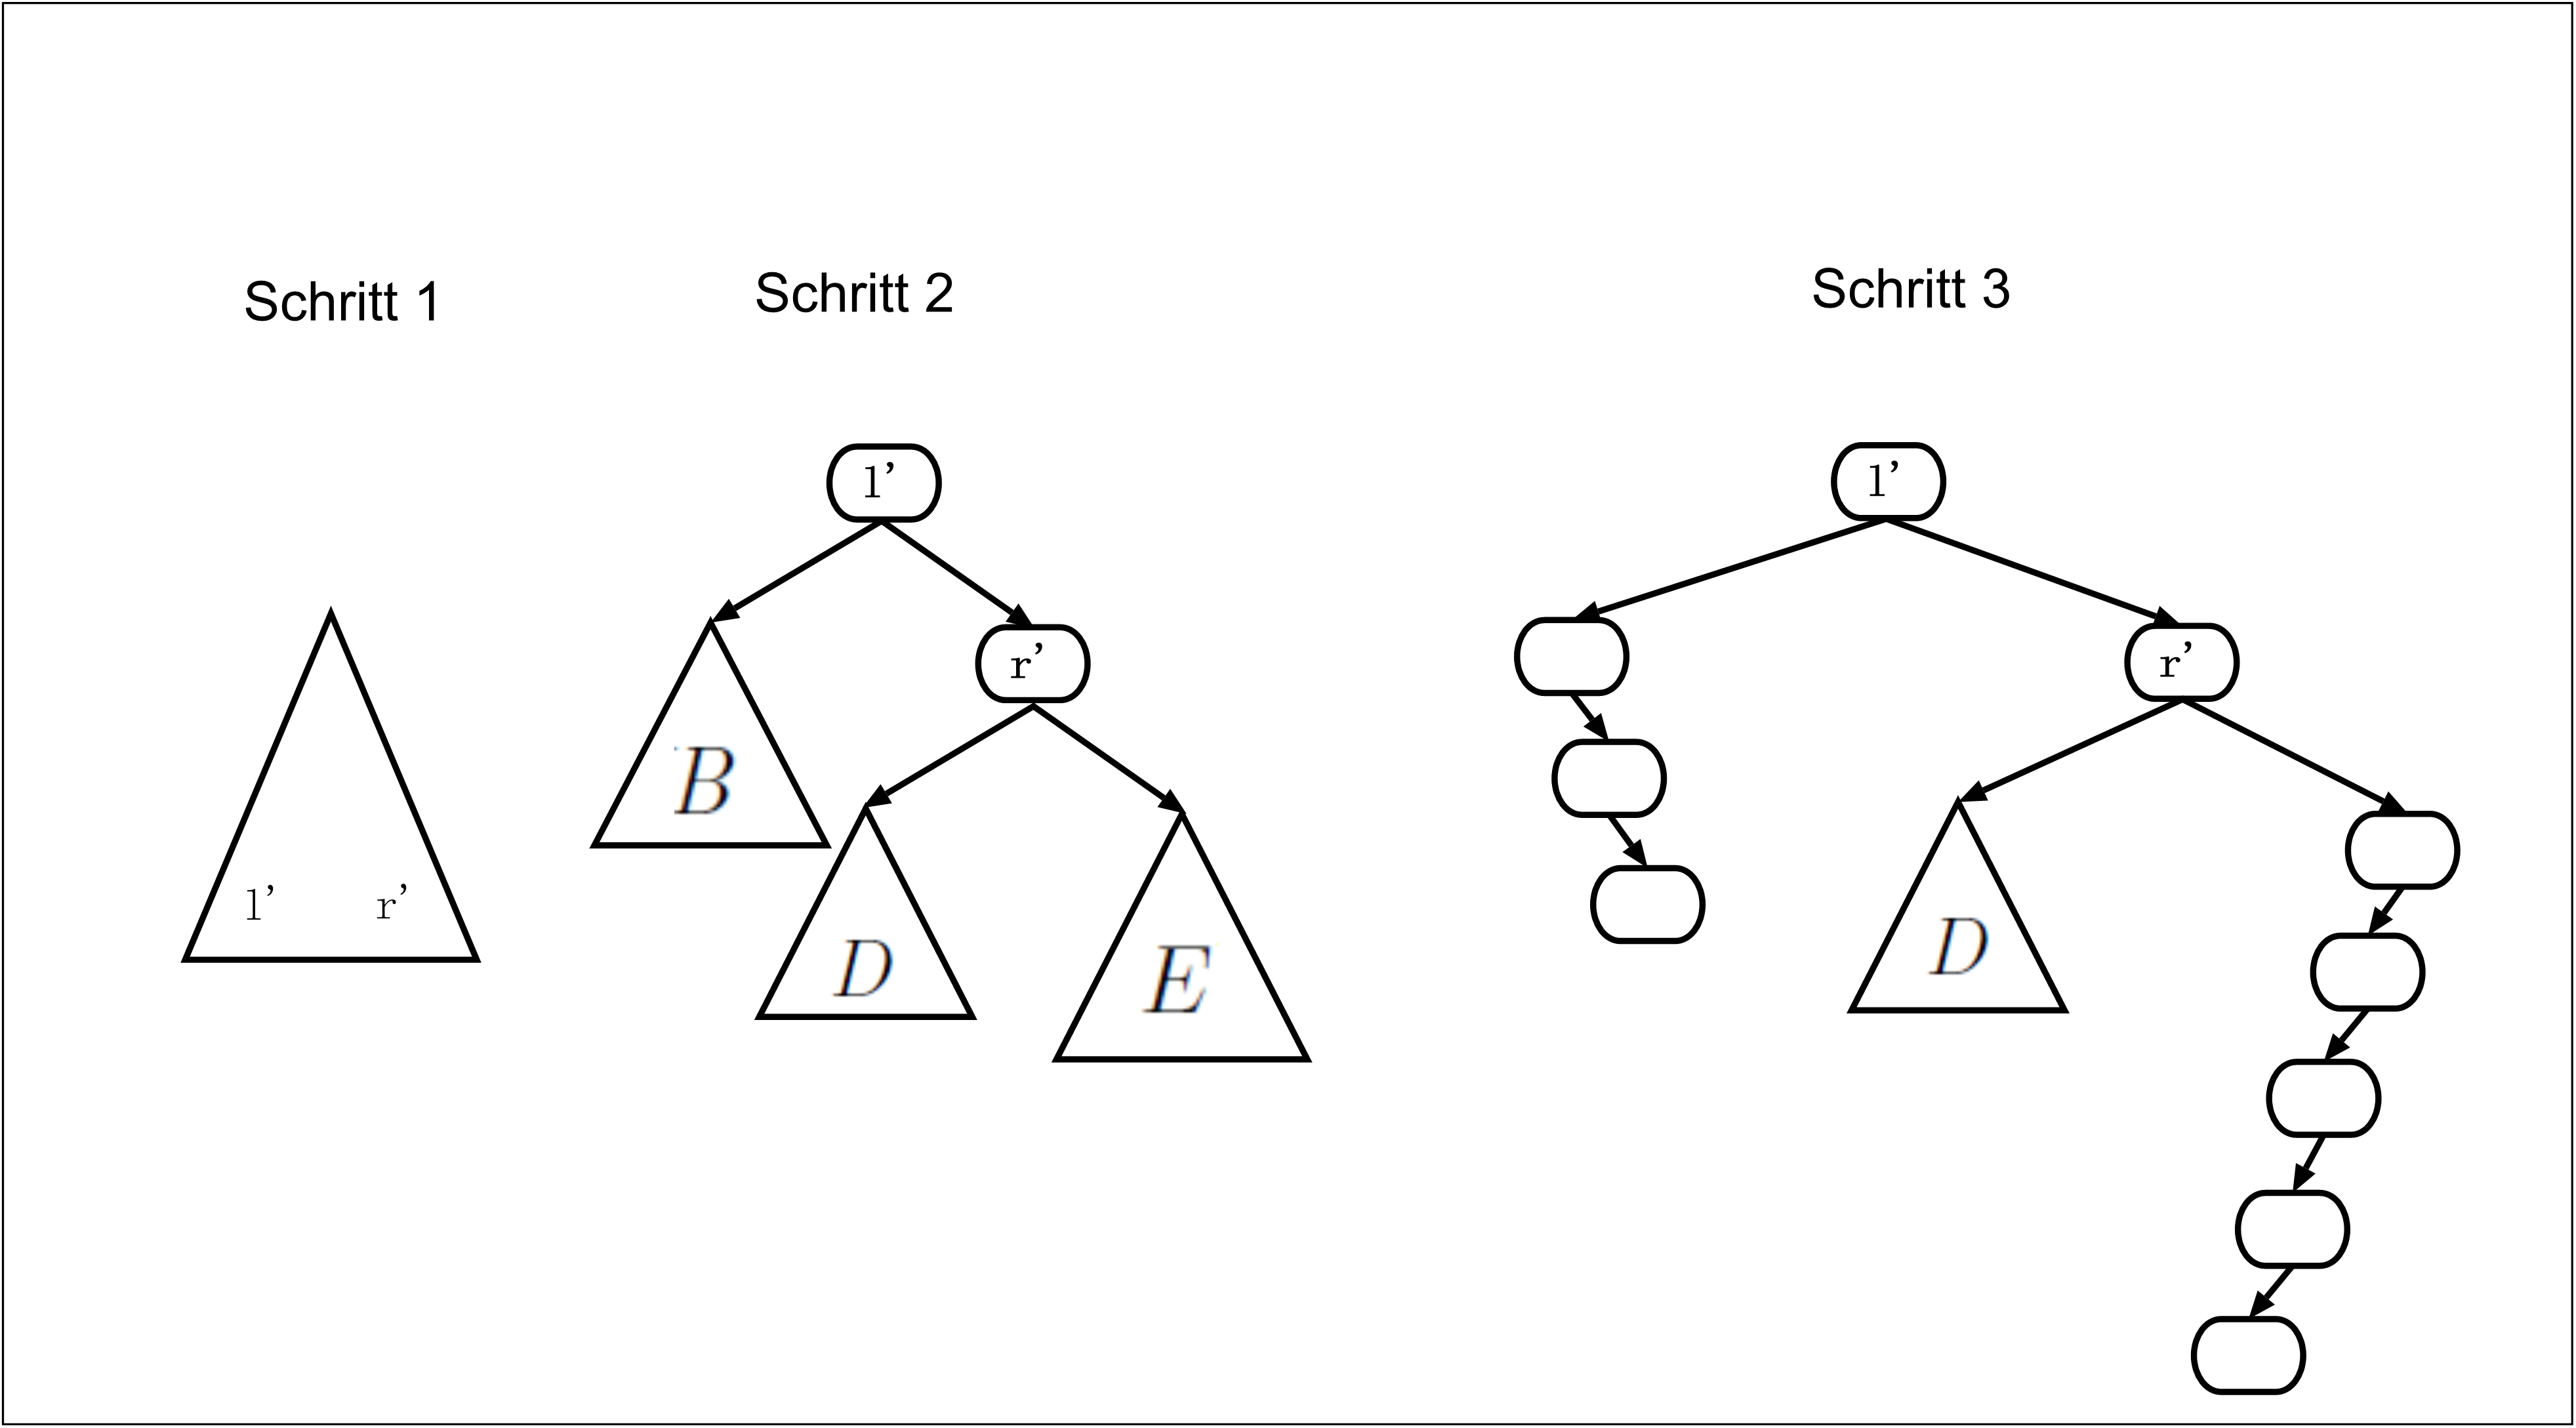
\includegraphics[height= 0.5\textwidth]{Medien/Zipper/hybrid/extractHybrid}
	\caption{Extraktionsprozess beim Zipper Baum. }
	\label{fig:extractHybrid}
\end{figure}
\subsection{Multisplay Baum}
Ein preferred path wird hier durch einen Splay Baum dargestellt, um dessen Laufzeiteigenschaften nutzen zu können. Da der Splay Baum kein balancierter BST ist, gibt es zusätzliche mögliche Zustände im Vergleich zu einem Tango Baum mit der gleichen Knotenzahl. Die Darstellung des Hilfsbaumes mit der Wurzel des Gesamtbaumes in Abbildung \ref{fig:pfadRepresentation}, wäre so beim Tango Baum nicht möglich. Zu den genannten Eigenschaften bezüglich der Laufzeit sind Beweise in \cite{multisplay} enthalten. Der Multisplay Baum erfüllt die Working Set Property \cite{porpMultiSplay}. 
\begin{figure}[H]
	\centering
	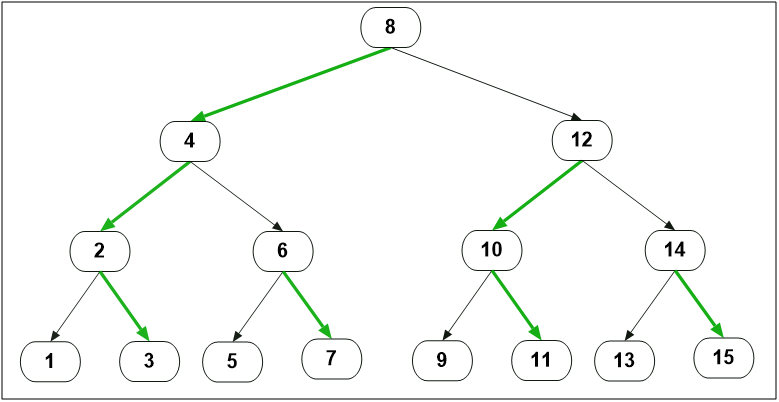
\includegraphics[width= 0.8\textwidth]{Medien/Multisplay/referenzTree}
	\caption {Referenzbaum mit grün gezeichneten preferred paths. }
	\label{fig:referenzTree}
\end{figure} 
\begin{figure}[H]
	\centering
	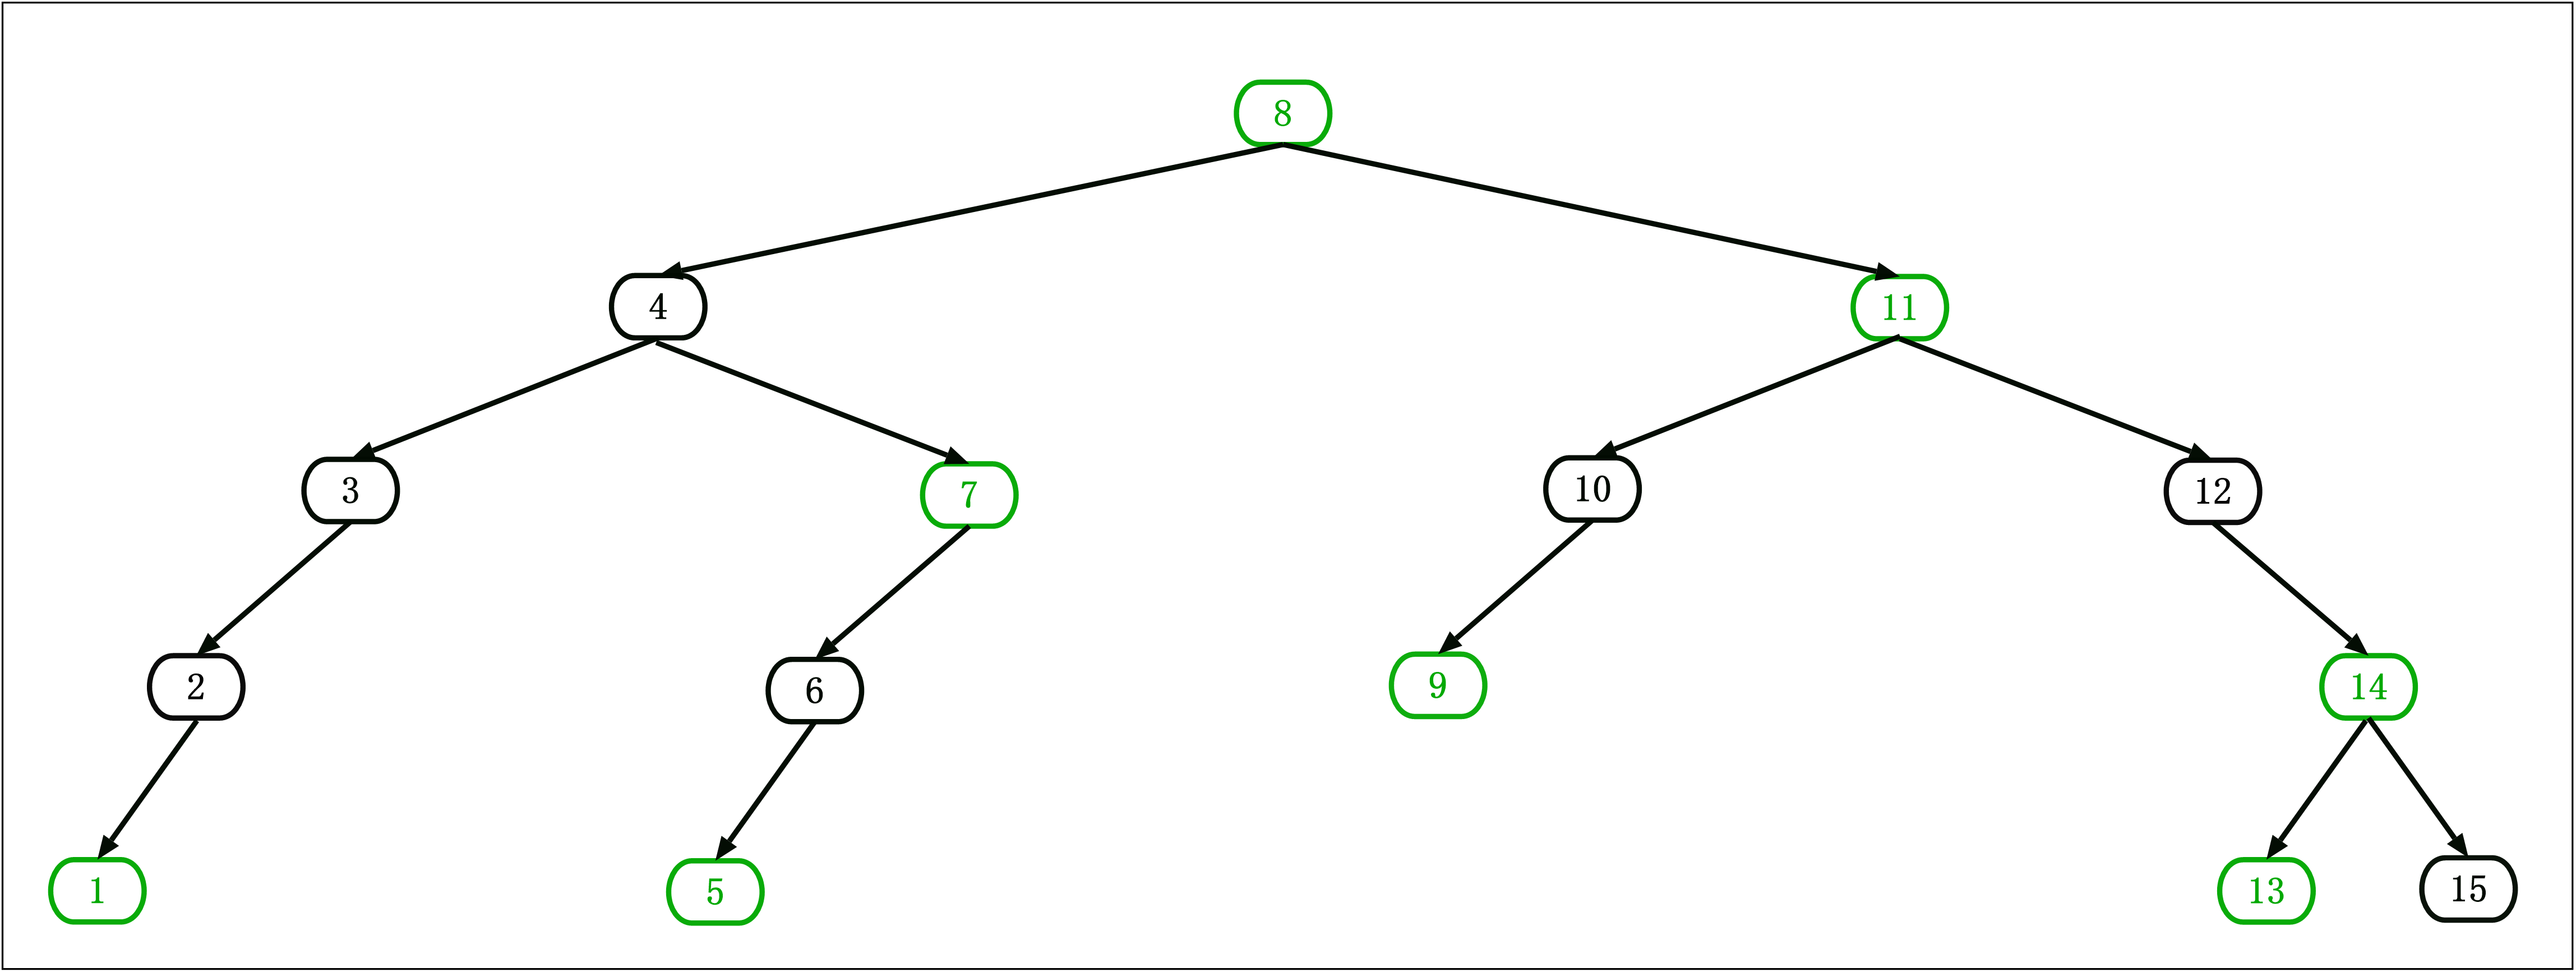
\includegraphics[width= 1\textwidth]{Medien/Multisplay/pfadRepresentation}
	\caption {Beispielhafter Multisplay Baum zum Referenzbaum aus Abbildung \ref{fig:referenzTree}.}
	\label{fig:pfadRepresentation}
\end{figure} 
\paragraph{Die \textit{access} Operation beim Multisplay Baum:}
Zu beachten ist, dass jede BST Darstellung auch eine Splay Baum Darstellung ist. Anders als beim Tango oder Zipper Baum muss ein neu erzeugter Hilfsbaum also nicht so angepasst werden, dass er weitere Invarianten einhält. Nach einer \textit{access}$\left(k\right)$ Operation ist der Knoten $v_k$ mit dem Schlüssel $k$ die Wurzel des Multisplay Baumes $T$. Zunächst wird eine gewöhnliche Suche in $T$ durchgeführt, bis der Zeiger $p$ der Operation auf $v_k$ zeigt. Ist $v_k$ gefunden, werden die Pfadrepräsentationen aktualisiert. Hierzu muss der Hilfsbaum, der die Wurzel von $T$ enthält neu erzeugt werden. \textit{cut} und \textit{join} werden beim Multisplay Baum zu \textit{switch} zusammengefasst. Zum Erzeugen des neuen Hilfsbaumes mit der Wurzel des Gesamtbaumes sind so viele \textit{switch} Operationen notwendig, wie es Wechsel bei preferred children gab.  \\

\section{Dokumentation zur Implementierung}
In diesem Kapitel wird die Implementierung zum Tango Baum beschrieben. 
Implementiert wurde der Tango Baum mit dem Rot-Schwarz-Baum als Hilfsdatenstruktur. Außerdem wurde der Splay Baum implementiert, um Laufzeittests zwischen diesem und dem Tango Baum durchführen zu können. Bedient werden kann das Programm über eine einfach gehaltene graphische Oberfläche. Das Programm wurde mit Java 8 übersetzt und als IDE wurde Apache NetBeans 12.0 verwendet. 
\begin{figure}[H]
	\centering
	\includegraphics[width= 1\textwidth]{Medien/laufzeittest/MainGUI}
	\caption{Sreenshot des Hauptfensters der GUI. Im oberen Teil befindet sich der Referenzbaum. Im unteren Teil der dazugehörige Tango Baum.}
	\label{fig:TangoBaumGui}
\end{figure}

\noindent Abbildung \ref{fig:TangoBaumGui} zeigt das Hauptfenster. Oben ist ein Referenzbaum zu einem Tango Baum mit  $15$ Knoten dargestellt, unten der Tango Baum. Preferred children und die Wurzeln von Hilfsbäumen sind grün dargestellt.
Diese Ansicht dient dazu, die Beziehung zwischen dem Referenzbaum und dem Tango Baum darzustellen.

\begin{figure}[H]
	\centering
	\includegraphics[width=0.3\textwidth]{Medien/laufzeittest/accessGUI}
	\caption{Mit diesem Fenster können  \textit{access} Operationen auf dem Tango Baum des Hauptfensters angestoßen werden.}
	\label{fig:accessGui}
\end{figure}
\noindent Mit dem Menüpunkt \enquote{access} wird das Fenster aus Abbildung \ref{fig:accessGui} geöffnet. Mit diesem werden \textit{access} Operationen angestoßen. Außerdem können die Bäume damit zurückgesetzt werden.

\begin{figure}[H]
	\centering
	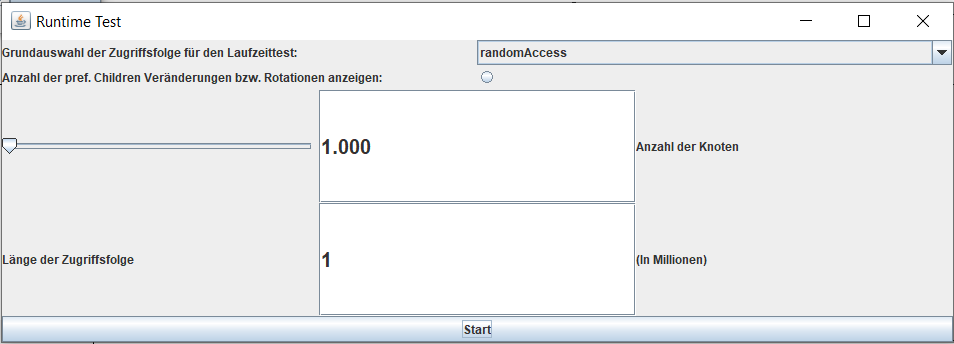
\includegraphics[width=1\textwidth]{Medien/laufzeittest/RuntimeGui}
	\caption{Mit diesem Fenster kann ein Laufzeittest ausgewählt, parametriert und angestoßen werden.}
	\label{fig:RuntimeGui}
\end{figure}

\noindent Mit dem Menüpunkt \enquote{RuntimeTest} wird das Fenster aus Abbildung \ref{fig:RuntimeGui} geöffnet. Mit diesem können Laufzeittests zwischen dem Tango Baum und dem Splay Baum  durchgeführt werden. Auf die Parameter und den Aufbau der Zugriffsfolgen wird im Abschnitt zu den Laufzeittests eingegangen. Ungültige Werte, also z. B. eine negative Anzahl an Knoten, werden von den Eingabeelementen nicht angenommen, sondern mit dem letzten gültigen Wert überschrieben.


\begin{figure}[H]
	\centering
	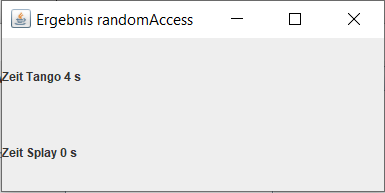
\includegraphics[width=0.8\textwidth]{Medien/laufzeittest/ResultGUI}
	\caption{Mit diesem Fenster wird das Resultat eines Laufzeittests dargestellt.}
	\label{fig:ResultGUI}
\end{figure}


\begin{figure}[H]
	\centering
	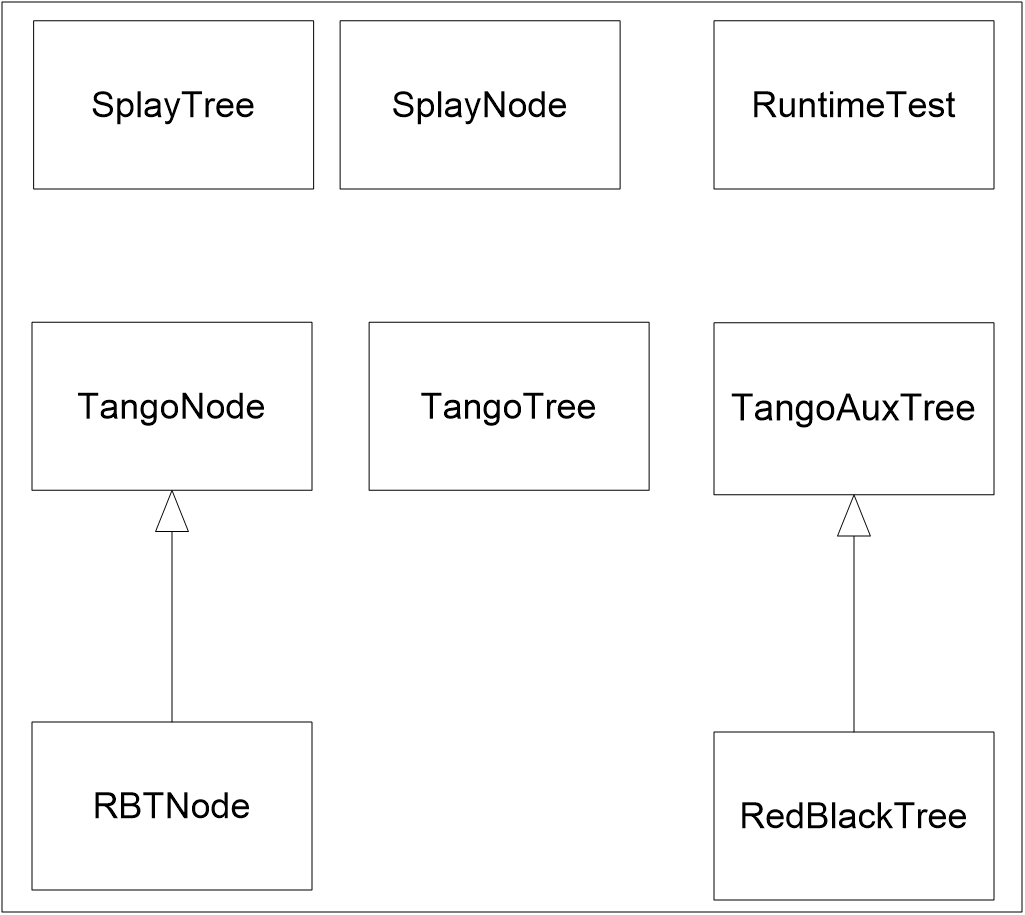
\includegraphics[width=1\textwidth]{Medien/laufzeittest/klassen}
	\caption{Wesentliche Klassen der Implementierung. Methoden zum direkten Lesen, bzw. Schreiben von Attributen sind nicht dargestellt. }
	\label{fig:klassen}
\end{figure}

\subsection{Beschreibung der Klassen }
Abbildung \ref{fig:klassen} stellt das Klassendiagramm zur Implementierung dar. Die einzelnen Klassen werden nun noch genauer beschrieben.
\paragraph{SplayTree und SplayNode:}
Der Splay Baum startet genau wie der Tango Baum vollständig balanciert, obwohl sich dies bei längeren Zugriffsfolgen praktisch nicht auswirken sollte. Ansonsten gibt es keine Besonderheiten. \textit{access} verhält sich genauso wie im Kapitel zum Splay Baum beschrieben. 

\paragraph{TangoNode:}
Der TangoNode enthält bereits alle zwingend notwendigen Attribute eines Knotens im Tango Baum. 

\paragraph{TangoAuxTree:}
Klassen, deren Objekte als Hilfsbaum im Tango Baum eingesetzt werden sollen, müssen diese Klasse erweitern. \textit{setTree} wird benötigt, da von der Klasse TangoTree abgeleitete Objekte ihre BST Struktur nur über das Attribut \enquote{auxTree} erreichen. Gibt es eine Veränderung an der Wurzel des Tango Baumes, wird die BST Struktur von \enquote{auxTree} neu gesetzt. Da ein Objekt das einen BST repräsentiert die eigentliche BST Struktur im Normalfall nur über ein Attribut \textit{root} erreicht, sollte diese zusätzliche Anforderung einfach zu erfüllen sein. \textit{updateDepthsPath} pflegt die Attribute \enquote{minDepth} und \enquote{maxDepth} der TangoNode.

\paragraph{TangoTree:}
\enquote{auxTree} macht die Wurzel des Tango Baumes erreichbar. Außerdem können über dieses Attribut die \textit{split} und \textit{concatenate} Operationen aufgerufen werden. \enquote{auxTreeClass} entspricht der Klasse, deren  Objekte Hilfsbäume eingesetzt werden. Diese wird dem Constructor übergeben. Somit kann der RBT einfach durch eine andere geeignete Struktur ersetzt werden.

\paragraph{RedBlackTree und RBTNode:}
Diese erweitern die abstrakten Klassen TangoAuxTree und TangoNode. RedBlackTree verhält sich wie im Kapitel zum Rot-Schwarz-Baum  beschrieben. 

\paragraph{RuntimeTest:}
 Klassen deren Objekte einen Laufzeittest mit dem Tango Baum und dem Splay Baum durchführen sollen, müssen diese Klasse erweitern. Das Attribut \enquote{exit} wird über die GUI gesetzt, worauf hin ein gestarteter Test abgebrochen wird. Die Methode \textit{runtimeTest} führt den eigentlichen Test durch und gibt ein Array mit der maximalen Länge vier zurück. Dieses enthält dann die Ausführungszeiten des Tango Baumes und des Splay Baumes, sowie die Anzahl der Veränderungen bei preferred Children im Referenzbaum zum Tango Baum und die Anzahl der vom Splay Baum ausgeführten Rotationen. Um Programmabbrüchen aufgrund zu wenig Speicher vorzubeugen, wurde bei den Projekteigenschaften die Option \enquote{ -Xmx4096m} gesetzt, Abbildung \ref{fig:optionSpeicher}.
 
 \paragraph{RandomTest:}
Diese Klasse erweitert die Klasse RuntimeTest. Insgesamt sind in dem Projekt sechs solcher Klassen vorhanden. Prinzipiell unterscheiden diese sich jedoch nicht, weshalb hier nur exemplarisch auf eine dieser Klasse eingegangen wird. Die Methode \textit{startTest} erzeugt eine Zugriffsfolge, bei der jeder enthaltene Schlüssel durch einen Pseudozufallsgenerator ausgewählt wurde. Der Test selbst wird dann von der bereits in der Klasse RuntimeTest implementierten Methode \textit{runtimeTest} ausgeführt. 
 
\begin{figure}[H]
	\centering
	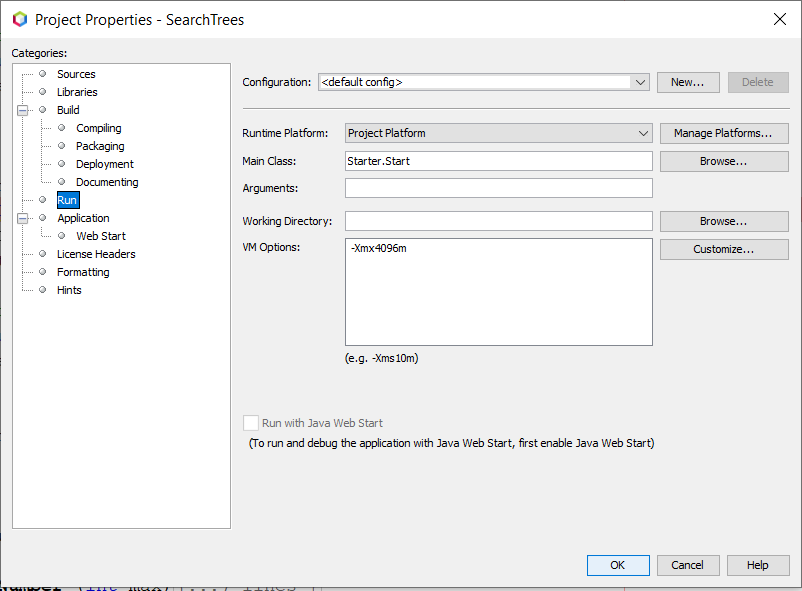
\includegraphics[width=1\textwidth]{Medien/laufzeittest/optionSpeicher}
	\caption{Den zur Ausführung verwendbaren Speicher auf 4096MB erweitern.}
	\label{fig:optionSpeicher}
\end{figure}


\section {Laufzeittests mit dem Tango Baum und dem Splay Baum.}

Es werden Laufzeittests zu unterschiedlichen Arten von Zugriffsfolgen durchgeführt. Unter anderem solche, die auf eine der Eigenschaften  Static Finger,  Working Set oder Dynamic Finger aus Abschnitt \ref{upperBounds} zugeschnitten sind. Hierzu werden dann Zugriffsfolgen verwendet, bei denen die jeweilige Eigenschaft für die Laufzeit besonders relevant ist. Der Tango Baum erfüllt die aufgeführten Eigenschaften zwar nicht, jedoch ist er  $\log\left(\log\left(n\right)\right)$-competitive. Ein dynamisch optimaler BST muss diese Eigenschaften erfüllen. Dadurch könnte auch der Tango Baum von den speziellen Eigenschaften der Zugriffsfolgen indirekt profitieren.  \\

\subsection{Verwendete Zugriffsfolgen zu den Laufzeittests.}
Hier werden die verwendeten Zugriffsfolgen zunächst kurz vorgestellt. Auf Details zum Aufbau wird dann im Abschnitt zu dem  jeweiligen Test eingegangen. $n$ entspricht der Anzahl der Knoten und $m$ der Länge der Zugriffsfolge. Als Schlüsselmenge wird $K = \{1,2,..,n\}$ verwendet. Existiert keine Abhängigkeit von $m$ zu $n$, so haben die Zugriffsfolgen die Länge $40$ Millionen. 

 \begin{enumerate}
 	\item Zufällig erzeugte Zugriffsfolgen.
 	\item Die Bit Reversal Permutation:\\
 	Es werden mehrere solcher in Abschnitt \ref{abschnittBitReversal} beschriebenen Zugriffsfolgen mit unterschiedlich langen Binärdarstellungen der Schlüssel verwendet.
 	\item Zugriffsfolgen zur Static Finger Property: \\
    Hier wird ein Schlüssel $k_F \in K$ gewählt. Die Häufigkeit des Vorkommens eines Schlüssels $k \in K$ in $X$ ist von $\vert k - k_F \vert$ abhängig. Schlüssel zu denen dieser Wert klein ist, sind häufiger enthalten als andere. Es werden solche Zugriffsfolgen für Schlüsselmengen mit unterschiedlicher Kardinalität erstellt und die Ergebnisse der beiden Datenstrukturen verglichen. Zusätzlich werden noch Zugriffsfolgen $X_1, X_2,.., X_7$ verwendet, so dass die Static Finger Property mit steigendem Index der Zugriffsfolge relevanter wird. Bei diesen sieben Folgen ist der Wert für $n$ konstant.
 	 \item Zugriffsfolgen zur Dynamic Finger Property:\\
 	Hier werden Zugriffsfolgen verwendet, so dass $\vert x_{i+1} - x_{i} \vert$ für alle \\
 	 \mbox{$i \in \{1, 2,..,m -1\} $} einen festen parametrierbaren Wert ergibt.  Zusätzlich werden noch Zugriffsfolgen $X_1, X_2,.., X_7$ verwendet, so dass die Dynamic Finger Property mit steigendem Index der Zugriffsfolge weniger relevant wird.
 	\item Zugriffsfolgen zur Working Set Property:\\
 	In den hier verwendeten Zugriffsfolgen wiederholen sich die Schlüssel mit einem festen parametrierbaren Abstand. Um Einflüsse der anderen aufgeführten Eigenschaften niedrig zu halten, werden die verwendeten Schlüssel betragsmäßig über die gesamte Schlüsselmenge verteilt. Außerdem gilt für zwei aufeinanderfolgende Schlüssel $k_1$ und $k_2$ in den meisten Fällen $\vert k_1 - k_2 \vert = n /2$. Zusätzlich werden noch Zugriffsfolgen $X_1, X_2,.., X_7$ verwendet, mit denen analog zur Dynamic Finger Property vorgegangen wird.
  \item Alternierend die Schlüssel $1$ und $n$.
  \item Aufsteigend sortiert:\\
  Jeder Schlüssel wird nur einmal verwendet.
  \item Absteigend sortiert:\\
  Jeder Schlüssel wird nur einmal verwendet.
  \item  Alternierend aufsteigend und absteigend sortiert:\\
   Jeder Schlüssel wird zweimal verwendet.
 \end{enumerate}



\subsection{Durchführung der Laufzeittests.} 
Hier werden die verwendetetn Zugriffsfolgen  im Detail beschrieben. Außerdem werden die Ergebnisse der Laufzeittests vorgestellt.
\subsubsection{Zufällig erzeugte Zugriffsfolgen}
	Ein Pseudozufallsgenerator erstellt die hier verwendeten Zugriffsfolgen. Für jedes $i \in \{1,2..,m\}$ und $k \in K$ ist die Wahrscheinlichkeit, dass $x_i = k$ gilt, gleich $1 /n$. Es werden jeweils zehn solche Zugriffsfolgen pro verwendeter Schlüsselmenge getestet. \label{zufZu} \\
	Als erstes werden die Zeiten zu den Zugriffsfolgen dargestellt, bei denen der Tango Baum die kürzesten Laufzeiten erreichte:

\begin{figure}[H]
	\centering
	\includegraphics[width=0.7\textwidth]{Medien/laufzeittest/diagramm/randomaccess1}
	\caption{Ergebnisse zu den zufällig erzeugten Zugriffsfolgen, mit den kürzesten Laufzeiten des Tango Baumes.}
 	
\end{figure}
\begin{table}[H]
	\begin{center}
		\begin{tabular}[c]{|c|c|c|}
			\hline
			$n$ & Zeit Tango in $\left(s\right)$ &Zeit Splay in $\left(s\right)$ \\
			\hline
			$10^3$ & $138,2$ &$6,5$ \\
			\hline
			$10^4$  & $235,6$ &$9,9$  \\
			\hline
			$10^5$  & $328,6$ &$15,1$  \\
			\hline
			$10^6$  & $465,7$ &$31,4$  \\
			\hline
			$10^7$  & $1557,3$ &$53$  \\
			\hline
		\end{tabular}
		\caption{Ergebnisse zu den zufällig erzeugten Zugriffsfolgen, mit den kürzesten Laufzeiten des Tango Baumes.} 
	\end{center}
\end{table}
\noindent	Hier werden die Zeiten zu den Zugriffsfolgen dargestellt, bei denen der Splay Baum die kürzesten  Laufzeiten erreichte:
\begin{figure}[H]
	\centering
	\includegraphics[width=0.7\textwidth]{Medien/laufzeittest/diagramm/randomaccess2}
	\caption{Ergebnisse zu den zufällig erzeugten Zugriffsfolgen, mit den kürzesten Laufzeiten des Splay Baumes.}
	
\end{figure}
\begin{table}[H]
	\begin{center}
		\begin{tabular}[c]{|c|c|c|}
			\hline
			$n$ & Zeit Tango in $\left(s\right)$ &Zeit Splay in $\left(s\right)$ \\
			\hline
			$10^3$ & $143,4$ &$6$ \\
			\hline
			$10^4$  & $235,6$ &$9,9$  \\
			\hline
			$10^5$  & $328,6$ &$15,1$  \\
			\hline
			$10^6$  & $465,7$ &$31,4$  \\
			\hline
			$10^7$  & $1569,3$ &$52,5$  \\
			\hline
		\end{tabular}
		\caption{Ergebnisse zu den zufällig erzeugten Zugriffsfolgen, mit den kürzesten Laufzeiten des Splay Baumes.} 
	\end{center}
\end{table}

\noindent Hier werden die durchschnittlichen Werte über jeweils zehn Zugriffsfolgen dargestellt:
\begin{figure}[H]
	\centering
	\includegraphics[width=0.7\textwidth]{Medien/laufzeittest/diagramm/randomaccess3}
	\caption{Durchschnittliche Laufzeiten zu jeweils zehn zufällig erzeugten Zugriffsfolgen.}
	
\end{figure}
\begin{table}[H]
	\begin{center}
		\begin{tabular}[c]{|c|c|c|}
			\hline
			$n$ & Zeit Tango in $\left(s\right)$ &Zeit Splay in $\left(s\right)$ \\
			\hline
			$10^3$ & $198,3$ &$8$ \\
			\hline
			$10^4$  & $483,1$ &$20.3$  \\
			\hline
			$10^5$  & $438$ &$17,7$  \\
			\hline
			$10^6$  & $470,8$ &$32,7$  \\
			\hline
			$10^7$  & $1613,5$ &$53,7$  \\
			\hline
		\end{tabular}
		\caption{Durchschnittliche Laufzeiten zu jeweils zehn zufällig erzeugten Zugriffsfolgen.} 
	\end{center}
\end{table}
\noindent Beide erreichen bei diesen Zugriffsfolgen im Vergleich zu den meisten noch Folgenden hohe Werte bei der Laufzeit. Da es sich um dynamische BST handelt, ist dies auch zu erwarten. Der Zustand der dynamischen BSTs wird im Wesentlichen durch  die  bereits ausgeführten \textit{access} Operationen bestimmt. Bei den hier verwendeten Zugriffsfolgen gibt es keine Abhängigkeiten zwischen dem Parameter einer \textit{access} Operation, zu denen von bereits ausgeführter \textit{access} Operationen. Somit kann durch die Anpassung des Zustandes kein genereller Vorteil generiert werden.\\
Jetzt wird noch auf die deutlichen Differenzen zwischen den Werten des Tango Baumes und des Splay Baumes eingegangen. Die Laufzeit des Tango Baumes ist im Wesentlichen von der Gesamtanzahl der Veränderungen  bei preferred children $n_T$ in seinem Referenzbaum  abhängig. Die Laufzeit des Splay Baumes ist im Wesentlichen von der Anzahl der ausgeführten Rotationen $n_S$ abhängig. Die Tabelle \ref{tab:Ran} stellt die durchschnittlichen Werte von $n_T$ und $n_S$ über jeweils zehn Zugriffsfolgen gegenüber.    
\begin{table}[H] 
	\begin{center}
		\begin{tabular}	[c]{|c|c|c|c|}  
			\hline
			$n$ & $n_T$ & $n_S$ & $n_T / n_S$\\
			\hline
			$10^3$ & $167.247.550$ &$456.650.373$ &$0,37$\\
			\hline
			$10^4$  & $233.092.762$ &$649.066.234$&$0,36$  \\
			\hline
			$10^5$  & $299.550.021$ &$842.015.806$ & $0,36$\\
			\hline
			$10^6$  & $367.122.698$ &$1.034.934.019$ & $0,35$\\
			\hline
			$10^7$  & $439.981.567$ &$1.226.490.084$ & $0,36$\\
			\hline
		\end{tabular}
		\caption{Die Spalte $n_T$ enthält die durchschnittliche Anzahl der Veränderungen bei preferred children im Referenzbaum zum Tango Baum über zehn Zugriffsfolgen. Die Spalte $n_S$ enthält die durchschnittliche Anzahl der Rotationen beim Splay Baum über zehn Zugriffsfolgen.   }  
		\label{tab:Ran}
	\end{center}
\end{table}
\noindent In der Spalte $a = n_T / n_S$ gibt es  keinen Wert $< 1/3$. Durchschnittlich muss der Splay Baum über die jeweils zehn Zugriffsfolgen, also maximal drei Rotationen pro Veränderung an einem preferred child durchführen. Der Tango Baum muss pro Veränderung an einem preferred child eine \textit{cut} und eine \textit{join} Operation ausführen. Dies führt im allgemeinen Fall zu vier \textit{split} und vier \textit{concatenate} Operationen,  die ausgeführt werden müssen. Für $n = 1000$ hat der Referenzbaum des Tango Baumes bereits zehn Ebenen, was in den meisten Fällen dazu führen wird, dass der Hilfsbaum mit der Wurzel des Tango Baumes neun oder zehn Knoten enthält. Es kann davon ausgegangen werden, dass das Ausführen der jeweils vier  \textit{split} und \textit{concatenate} Operationen deutlich aufwändiger ist, als das Ausführen der drei Rotationen, zumal aufgrund der \textit{insertFixup} Operation auch beim Tango Baum mehrere Rotationen pro Veränderung bei einem preferred child möglich sind. Abbildung \ref{fig:nT} stellt den Zusammenhang von $n_T$ und $n_S$ zu $n$ graphisch dar. 

\begin{figure}[H]
	\centering
	\includegraphics[width=0.7\textwidth]{Medien/laufzeittest/diagramm/nT}
	\caption{Hier sind $n_T$ und $n_S$ graphisch dargestellt.}
	\label{fig:nT}
\end{figure}
\noindent Der Aufwand, der nach einer Veränderung bei einem preferred child im Referenzbaum notwendig ist, um die Pfadrepräsentationen zu aktualisieren und die rote Kennlinie in Abbildung \ref{fig:nT} lassen annehmen, dass der Tango Baum für Schlüsselmengen konstruiert wurde, deren Kardinalitäten deutlich größer sind, als die hier darstellbaren. \\
 Allerdings ist $n_T/ n_S$ bei den hier durchgeführten Tests in etwa konstant. Für die Kosten zum  Aktualisieren einer Pfadrepräsentation im Tango Baum gilt $O\left(\log\left(\log\left(n\right)\right)\right)$ und die Kosten zum Ausführen einer Rotation sind unabhängig von $n$. Kombiniert mit der bewiesenen $\log\left(\log\left(n\right)\right)$-competitiveness des Tango Baumes ergibt sich hier ein (vorsichtiger) Hinweis auf die dynamische Optimalität des Splay Baumes.
\subsubsection{Bit Reversal Permutations}
Auf der X-Achse wird die Länge der Binärdarstellung der Schlüssel $l$ dargestellt. In der Spalte $2^l$ kann die Länge der Zugriffsfolge und die Anzahl der Knoten abgelesen werden. 
\begin{figure}[H]
	\centering
	\includegraphics[width=0.7\textwidth]{Medien/laufzeittest/diagramm/brp}
	\caption{Ergebnisse zu den Laufzeittests zur Bit Reversal Permutation.}
	\label{fig:ResultGUI}
\end{figure}
\begin{table}[H]
	\begin{center}
		\begin{tabular}[c]{|c|c|c|c|}
			\hline
			$l$ & $2^l$ &Zeit Tango in $\left(s\right)$ &Zeit Splay in $\left(s\right)$ \\
			\hline
			$17$ &	$131.072 $ &$2,2$ &$0,1$ \\
			\hline
			$18$  &$262.144 $ &$4,1$ &$0,3$  \\
			\hline
			$19$  &$524.288 $ &$12,1$ &$1,7$  \\
			\hline
			$20$  &$1.048.576 $ &$45,7$ &$3,5$  \\
			\hline
			$21$  &$2.097.152 $ &$98,9$ &$5,5$  \\
			\hline
			$22$  &$4.194.304 $ &$140,3$ &$12,8$  \\
			\hline
			$23$  &$8.388.608 $ &$258,2$ &$20,7$  \\
			\hline
			$24$  &$16.777.216$ &$457,3$ &$35$  \\
			\hline
		\end{tabular}
		\caption{Ergebnisse zu den Laufzeittests zur Bit Reversal Permutation.} 
	\end{center}
\end{table}
\noindent Wie in Abschnitt \ref{abschnittBitReversal} gezeigt, gilt bei diesen Folgen für die Laufzeit eines beliebigen BSTs, $\Omega \left(n \log\left(n\right)\right)$. Der Splay Baum erfüllt die Balanced Property, weshalb für seine Laufzeit auch $O\left(n + n \log\left(n\right)\right)$ gelten muss. Die Ergebnisse bestätigen, dass es sich um aufwändige Zugriffsfolgen für BSTs handelt. Vergleichbare Werte traten nur bei den zufällig erzeugten Zugriffsfolgen auf. \\




\subsubsection{Static Finger Property}
Sei $a = \lfloor n / 2\rfloor$.  $a$ ist der Parameter bei $2$ Prozent der \textit{access} Operationen. Auf $a+1$ und $a-1$ entfallen dann $1$ Prozent (gemeinsam $2$ Prozent) der restlichen \textit{access} Operationen. Dieses Vorgehen iteriert bis ein Prozent der Anzahl der verbleibenden \textit{access} Operationen weniger als $1$ ergibt. Es wird dann nochmals die Anzahl von Zugriffen auf $a$ hinzugefügt, die benötigt wird, um die gewünschte Länge der Zugriffsfolge zu erreichen. Die Anordnung der Schlüssel innerhalb der Zugriffsfolge erfolgt über einen Pseudozufallsgenerator. Da ein Pseudozufallsgenerator verwendet wird, werden zu jeder Schlüsselmenge wieder zehn Zugriffsfolgen erstellt. Anders als bei Anschnitt \ref{zufZu} erreichten beide BSTs ihre kürzeste Laufzeit jeweils bei der gleichen Zugriffsfolge, so dass diese in einem Diagramm dargestellt werden.\\ 
\begin{figure}[H]
	\centering
	\includegraphics[width=0.7\textwidth]{Medien/laufzeittest/diagramm/staticfinger1}
	\caption{Ergebnisse zu den Zugriffsfolgen zur Static Finger Property mit den kürzesten Laufzeiten beider BSTs.}
\end{figure}
\begin{table}[H]
	\begin{center}
		\begin{tabular}[c]{|c|c|c|}
			\hline
			$n$ & Zeit Tango in $\left(s\right)$ &Zeit Splay in $\left(s\right)$ \\
			\hline
			$10^3$ & $110.8$ &$4,6$ \\
			\hline
			$10^4$  & $121,3$ &$5$  \\
			\hline
			$10^5$  & $137$ &  $5,1$  \\
			\hline
			$10^6$  & $144,4$ &$4,9$  \\
			\hline
			$10^7$  & $125,8$ &$4,7$  \\
			\hline
		\end{tabular}
		\caption{Ergebnisse zu den Zugriffsfolgen zur Static Finger Property mit den kürzesten Laufzeiten beider BSTs.} 
	\end{center}
\end{table}

\begin{figure}[H]
	\centering
	\includegraphics[width=0.7\textwidth]{Medien/laufzeittest/diagramm/staticfinger3}
	\caption{Durchschnittliche Laufzeiten über jeweils zehn Zugriffsfolgen zur Static Finger Property.}
\end{figure}
\begin{table}[H]
	\begin{center}
		\begin{tabular}[c]{|c|c|c|}
			\hline
		$n$ & Zeit Tango in $\left(s\right)$ &Zeit Splay in $\left(s\right)$ \\
		\hline
		$10^3$ & $111.5$ &$5,1$ \\
		\hline
		$10^4$  & $125,3$ &$5,1$  \\
		\hline
		$10^5$  & $139,1$ &  $5,2$  \\
		\hline
		$10^6$  & $149,1$ &$5,1$  \\
		\hline
		$10^7$  & $128,2$ &$4,7$  \\
		\hline
		\end{tabular}
		\caption{Durchschnittliche Laufzeiten über jeweils zehn Zugriffsfolgen zur Static Finger Property.} 
	\end{center}
\end{table}
\noindent Sei $X$ eine der verwendeten Zugriffsfolgen und $L$ die Menge der in $X$ enthaltenen Schlüssel. $L$ hat eine Kardinalität von $968$. \\
Der Splay Baum erfüllt die Static Finger Property und zusätzlich führt die eingeschränkte Kardinalität von  $L$ gegenüber $K$ zu den niedrigen Laufzeiten.     
Auch der Tango Baum erreicht hier verglichen mit den weiter oben beschriebenen Laufzeittests kurze Laufzeiten. Die zu Beginn des Kapitels angeführte Vermutung, dass der Tango Baum aufgrund seiner $\log\left(\log\left(n\right)\right)$-competitiveness ebenfalls von den speziellen Eigenschaften solcher Zugriffsfolgen profitiert, bestätigt sich in diesem Fall. Auch hier kann zusätzlich die Kardinalität von $L$ zur Erklärung verwendet werden. Bei den größeren Instanzen wird sich das preferred child bei vielen Knoten im Referenzbaum zum Tango Baum entweder gar nicht oder nur bei wenigen \textit{access} Operationen ändern. \\

\noindent Nun werden Zugriffsfolgen für $n = 10.000.000$ verwendet. Es werden verschiedene Prozentsätze $p$ zum Berechnen der jeweiligen Anzahl des Vorkommens eines Schlüssels in der Zugriffsfolge verwendet. Pro Prozentsatz werden wieder die Durchschnittswerte zu zehn Zugriffsfolgen dargestellt. 
\begin{figure}[H]
	\centering
	\includegraphics[width=0.7\textwidth]{Medien/laufzeittest/diagramm/staticfinger4}
	\caption{Durchschnittliche Laufzeiten über jeweils zehn Zugriffsfolgen zur Static Finger Property mit variablem $p$.}
\end{figure}
\begin{table}[H]
	\begin{center}
		\begin{tabular}[c]{|c|c|c|}
			\hline
			$p$ in $\%$ & Zeit Tango in $\left(s\right)$ &Zeit Splay in $\left(s\right)$ \\
			\hline
			$2,5$  & $139,6$ &$5$  \\
			\hline
			$3$  &   $212,4$ &  $5,4$  \\
			\hline
			$3,5$  & $143$ &$5,4$  \\
			\hline
			$4$ &    $158$ &$4,8$ \\
			\hline
			$4,5$  & $110,7$ &$4,2$  \\
			\hline
			$5$  &   $105,8$ &  $3,9$  \\
			\hline
			$5,5$  & $111,5$ &$3,9$  \\
			\hline
		\end{tabular}
		\caption{Durchschnittliche Laufzeiten über jeweils zehn Zugriffsfolgen zur Static Finger Property mit variablem $p$.} 
	\end{center}
\end{table}

\noindent Die Laufzeiten des Splay Baumes werden erwartungsgemäß mit steigendem $p$ kürzer. Beim Tango Baum gibt es auch steigende Werte bei der Laufzeit, trotz steigenden Werten für $p$. Tendenziell werden aber auch seine Laufzeiten mit steigendem $p$ kürzer. Hier muss auch beachtet werden, dass wieder ein Pseudozufallsgenerator verwendet wurde.




\subsubsection{Dynamic Finger Property}
Im ersten Teil ist die Anzahl der Knoten wieder variabel und es werden Zugriffsfolgen der Form  $1, 3, 5,..,n-1, n-3, n-5, ..,1, 3, 5..., n-1,...$ verwendet. Die Differenz $a$ zwischen zwei aufeinanderfolgenden Schlüsseln ist \mbox{also $2$}.
\begin{figure}[H]
	\centering
	\includegraphics[width=0.7\textwidth]{Medien/laufzeittest/diagramm/dynamicfinger}
	\caption{Die Ergebnisse zum Laufzeittest zur Dynamic Finger Property mit \mbox{konstantem $a$.}}
\end{figure}
\begin{table}[H]
	\begin{center}
		\begin{tabular}[c]{|c|c|c|}
			\hline
			$n$ & Zeit Tango in $\left(s\right)$ &Zeit Splay in $\left(s\right)$ \\
			\hline
			$10^3$ & $58$ &$0,8$ \\
			\hline
			$10^4$  & $54,5$ &$1,7$  \\
			\hline
			$10^5$  & $68,4$ &$2,3$  \\
			\hline
			$10^6$  & $70,8$ &$4,4$  \\
			\hline
			$10^7$  & $81,1$ &$4,7$  \\
			\hline
			$1,6 *10^7$  & $83,3$ &$5,2$  \\
			\hline
		\end{tabular}
		\caption{Die Ergebnisse zum Laufzeittest zur Dynamic Finger Property mit \mbox{konstantem $a$.}} 
	\end{center}
\end{table}
\noindent Der Splay Baum erfüllt die Dynamic Finger Property und erreicht wie zu erwarten war, sehr kurze Laufzeiten. Auch der Tango Baum profitiert wieder von dem speziellem Aufbau der Zugriffsfolgen, wie an einem Vergleich der Laufzeiten zu den zufällig erzeugten Zugriffsfolgen erkennbar ist. 


\noindent Nun ist $n = 10.000.000$ fest und es werden unterschiedliche Werte für $a$ verwendet.

\begin{figure}[H]
	\centering
	\includegraphics[width=0.7\textwidth]{Medien/laufzeittest/diagramm/dynamicfingerNfest}
	\caption{Die Ergebnisse zum Laufzeittest zur Dynamic Finger Property mit variablem $a$.}
\end{figure}
\begin{table}[H]
	\begin{center}
		\begin{tabular}[c]{|c|c|c|}
			\hline
			$a$ & Zeit Tango in $\left(s\right)$ &Zeit Splay in $\left(s\right)$ \\
			\hline
			$2$ & $81,1$ &$4,7$ \\
			\hline
			$4$  & $108,6$ &$8,6$  \\
			\hline
			$8$  & $69$ &$14,8$  \\
			\hline
			$16$  & $63$ &$16,5$  \\
			\hline
			$32$  & $62,1$ &$16,8$  \\
			\hline
			$64$  & $63,8$ &$16,7$  \\
			\hline
			$128$  & $64,3$ &$16,7$  \\
			\hline
			$256$  & $88$ &$20,2$  \\
			\hline
		\end{tabular}
		\caption {Die Ergebnisse zum Laufzeittest zur Dynamic Finger Property mit variablem $a$.} 
	\end{center}
\end{table}\noindent Es ist zu erkennen, dass die Zeiten des Splay Baumes ansteigen, obwohl $n$ und $m$ konstant sind. Die Zeiten des Tango Baumes zeigen keine deutlich Tendenz, bleiben insgesamt jedoch vergleichsweise niedrig. Die Messwerte legen die Vermutung nahe, dass der Tango Baum von der konstanten Betragsdifferenz zweier aufeinanderfolgender Schlüssel profitiert. Es kann jedoch nicht abgeleitet werden, dass ein niedrigerer Wert bei $a$ auch zu kürzeren Laufzeiten führt.  



\subsubsection{Working Set Property} \label{testWork}
Die Schlüssel dieser Zugriffsfolgen wiederholen sich mit einem festem parametrierbaren Abstand $a$. 
Sei  $X = x_1, x_2,.., x_m$ eine verwendete Zugriffsfolge und $i \in \{1,2,..,m\}$. Sei $k$ ein Schlüssel mit $k = x_i$. Dann ist entweder $i-a$ der größte Index kleiner $i$, mit $x_{i-a} = k$ oder $i$ ist der kleinste Index mit $x_i = k$. Es werden die Teilmengen $t_0, t_1,.. t_b$ mit $b = n / a$, der  Schlüsselmenge gebildet. Sei $l \in \{0, 1,.., b\}$, $c = a/2$ und $d = n /2$, dann gilt: \\ $t_l = \{l * c + 1, l * c + 2,.., l * c + c\} \cup \{l * c + 1 + d, l * c + 2 + d,.., l * c + c + d\}$. Jede Teilmenge enthält also $a$ Elemente. Sei $e_1, e_2,.., e_c, e_{c+1}, e_{c+2},.., e_{c+c} $ die Folge aller in $t_l$ enthaltenen Elemente, aufsteigend sortiert nach dem Betrag. Aus $t_l$ wird eine Zugriffsfolge $s_l$ gebildet, indem  $e_1, e_{c+1}, e_2,e_{c+2}.., e_c, e_{c + c}$ so oft wiederholt wird, bis $s_l$ die Länge $m/b$ hat. Die Gesamtzugriffsfolge ist dann $s_0 \circ s_1 \circ...\circ s_l$. \\
Durch diesen Aufbau wird erreicht, dass zwar die Working Set Property für die Laufzeit relevant wird, die bereits betrachteten Eigenschaften jedoch nicht.\\
Im ersten Teil wird nun $a = 8$ gesetzt.

\begin{figure}[H]
	\centering
	\includegraphics[width=0.7\textwidth]{Medien/laufzeittest/diagramm/workingset}
	\caption{Die Ergebnisse zum Laufzeittest zur Working Set Property mit konstantem $a$.}
\end{figure}
\begin{table}[H]
	\begin{center}
		\begin{tabular}[c]{|c|c|c|}
			\hline
			$n$ & Zeit Tango in $\left(s\right)$ &Zeit Splay in $\left(s\right)$ \\
			\hline
			$10^3$ & $46,6$ &$0,9$ \\
			\hline
			$10^4$  & $45$ &$1$  \\
			\hline
			$10^5$  & $49,8$ &$1$  \\
			\hline
			$10^6$  & $48,1$ &$1$  \\
			\hline
			$10^7$  & $53,7$ &$1,2$  \\
			\hline
		\end{tabular}
		\caption{Die Ergebnisse zum Laufzeittest zur Working Set Property mit konstantem $a$.} 
	\end{center}
\end{table}
\noindent Beide BSTs erreichen hier ihre bisher kürzesten Laufzeiten. Zudem werden die Laufzeiten  bei steigendem $n$ nur etwas länger, trotz logarithmischer Skala zu $n$. Der Splay Baum erfüllt die Working Set Property, wodurch die kurzen Laufzeiten zu erklären sind. Nun wird eine mögliche Erklärung zum langsamen Ansteigen der Laufzeiten des Tango Baumes angegeben: \\
Seien $k_1, k_2$ und $k_3$ im Tango Baum enthaltene Schlüssel, so dass $k_1 + 1 = k_3$ und $k_2 \gg k_1$ gilt. Es wird aufeinanderfolgend \textit{access}$\left(k_1\right)$, \textit{access}$\left(k_2\right)$ und \\ \textit{access}$\left(k_3\right)$ ausgeführt. Betrachtet wird nun der Referenzbaum $P$ zum Tango Baum und \textit{access}$\left(k_3\right)$. Sei $P_k = p_1, p_2,.., p_l$ der Pfad von der Wurzel von $P$ zu dem Knoten $v_3$ mit dem Schlüssel $k_3$. Sei $v_v$ der gemeinsame Vorfahre von $v$ und dem Knoten $v_2$ mit dem Schlüssel $k_2$. $v_v$ muss der Knoten mit der kleinsten Tiefe sein, bei dem das preferred child wechselt (Eine Ausnahme ist $v_v = v_2$). Sei $u$ ein Knoten in $P_k$ mit größerer Tiefe als $v_v$, sowie \mbox{\textit{key}$\left(u\right) \neq k_1 \wedge $ \textit{key}$\left(u \right)\neq k_2 $}. Es muss entweder \textit{key}$\left(u\right) > k_3 > k_1$  oder  $ k_3 > k_1 >$\textit{key}$\left(u\right)$ gelten und somit müssen $k_1$ und $k_3$ im selben Teilbaum von $u$ enthalten sein. So kann erklärt werden, dass verlängerte Pfade im Referenzbaum hier nur zu wenigen zusätzlichen Veränderungen bei preferred children führen. \\  


\noindent Im zweiten Teil wird $n = 10.000.000$ gesetzt und $a$ ist variabel. 
\begin{figure}[H]
	\centering
	\includegraphics[width=0.7\textwidth]{Medien/laufzeittest/diagramm/workingset2}
	\caption{Die Ergebnisse zum Laufzeittest zur Working Set Property mit variablem $a$.}
\end{figure}
\begin{table}[H]
	\begin{center}
		\begin{tabular}[c]{|c|c|c|}
			\hline
			$a$ & Zeit Tango in $\left(s\right)$ &Zeit Splay in $\left(s\right)$ \\
			\hline
			$9$  & $67,8$ &$1,3$  \\
			\hline
			$11$  & $48,1$ &$1,4$  \\
			\hline
		    $13$  & $56$ &$1,6$  \\
			\hline
			$15$  & $60,6$ &$1,6$  \\
			\hline
			$17$  & $58$ &$1,7$  \\
			\hline
			$19$  & $60,8$ &$1,8$  \\
			\hline
			$21$  & $59,5$ &$2$  \\
			\hline
		\end{tabular}
		\caption{Die Ergebnisse zum Laufzeittest zur Working Set Property mit variablem $a$.} 
	\end{center}
\end{table}


\noindent Die Laufzeiten des Splay Baumes nehmen mit steigendem $a$ etwas größere Werte an, bleiben jedoch insgesamt kurz. Bei den Laufzeiten des Tango Baumes ist keine klare Tendenz auszumachen. Das bestätigt die Vermutung, dass der niedrige Betrag der Differenz der Parameter zweier \textit{access} Operationen, zwischen deren Ausführung nur eine weitere \textit{access} Operation liegt, wesentlich für die kurzen Laufzeiten ist.     
\newpage
\subsubsection{Weitere Laufzeittests}
\noindent \textbf{Alternierend die Schlüssel $1$ und $n$:\\}

\noindent Umgesetzt werden diese Zugriffsfolgen durch solche zur Dynamic Finger Property, bei denen $a = n -1$ für den Abstand $a$ gilt. Relevant für die Laufzeit wird hier jedoch die Working Set Property.

\begin{figure}[H]
	\centering
	\includegraphics[width=0.7\textwidth]{Medien/laufzeittest/diagramm/kleinGros}
	\caption{Laufzeittests, bei denen alternierend der kleinste und der größte Schlüssel verwendet wird.}
\end{figure}
\begin{table}[H]
	\begin{center}
		\begin{tabular}[c]{|c|c|c|}
			\hline
			$n$ & Zeit Tango in $\left(s\right)$ &Zeit Splay in $\left(s\right)$ \\
			\hline
			$10^3$ & $13$ &$0,4$ \\
			\hline
			$10^4$  & $14,7$ &$0,5$  \\
			\hline
			$10^5$  & $27,7$ &$1,1$  \\
			\hline
			$10^6$  & $35,3$ &$0,9$  \\
			\hline
			$10^7$  & $44,2$ &$1$  \\
			\hline
			$1,6 *10^7$  & $46,3$ &$1$  \\
			\hline
		\end{tabular}
		\caption{Laufzeittests, bei denen alternierend der kleinste und der größte Schlüssel verwendet wird.} 
	\end{center}
\end{table}
\noindent Beide BSTs erreichen hier ihre bisher kürzesten Laufzeiten. Dies war auch zu erwarten. Im Referenzbaum zum Tango Baum wird es ab der dritten \textit{access} Operation, pro Operation nur noch zu einem Wechsel des preferred child an der Wurzel kommen. Beim Splay Baum ist der Knoten mit dem größten Schlüssel nach der zweiten Operation an der Wurzel. Der Knoten mit dem kleinsten Schlüssel war nach der ersten Operation an der Wurzel. Somit sind ab der dritten Operation jeweils nur noch maximal zwei Rotationen notwendig. Zwei Rotationen sind der Fall, wenn bei der vorherigen Operation zum Abschluss zig-zig oder zag-zag angewendet wurde, siehe Abbildung \ref{fig:zigZag}.
 
 \bigskip

\noindent \textbf{Aufsteigend sortiert mit insgesamt $n$ Zugriffen:}\\
\bigskip
Zu beachten ist hier, dass die Dynamic Finger Property relevant wird. 

\begin{figure}[H]
	\centering
	\includegraphics[width=0.7\textwidth]{Medien/laufzeittest/diagramm/sorted1}
	\caption{Laufzeittests, bei denen aufsteigend sortierte Zugriffsfolgen verwendet werden.}
\end{figure}
\begin{table}[H]
	\begin{center}
		\begin{tabular}[c]{|c|c|c|}
			\hline
			$n$ & Zeit Tango in $\left(s\right)$ &Zeit Splay in $\left(s\right)$ \\
			\hline
			$10^3$ & $\approx 0$ &$\approx 0$ \\
			\hline
			$10^4$  & $0,1$ &$\approx 0$  \\
			\hline
			$10^5$  & $0,2$ &$\approx 0$  \\
			\hline
			$10^6$  & $1$ &$0,1$  \\
			\hline
			$10^7$  & $12.3$ &$0,3$  \\
			\hline
			$1,6 *10^7$  & $16.8$ &$0,4$  \\
			\hline
		\end{tabular}
		\caption{Laufzeittests, bei denen aufsteigend sortierte Zugriffsfolgen verwendet werden.} 
	\end{center}
\end{table}
\noindent Beide BSTs erreichten bei den Zugriffsfolgen zur Dynamic Finger Property  vergleichsweise kurze Laufzeiten. Hier kommt hinzu, dass die Länge der Zugriffsfolgen abhängig von der Anzahl der Knoten kürzer ist. Das Ergebnis sind erwartbar kurze Laufzeiten.
\newpage

\bigskip
\noindent \textbf{Absteigend sortiert mit insgesamt $n$ Zugriffen:\\}


\bigskip


\noindent Auch hier wird die Dynamic Finger Property relevant. 
\begin{figure}[H]
	\centering
	\includegraphics[width=0.7\textwidth]{Medien/laufzeittest/diagramm/sorted2}
	\caption{Laufzeittests, bei denen absteigend sortierte Zugriffsfolgen verwendet werden.}
\end{figure}
\begin{table}[H]
	\begin{center}
		\begin{tabular}[c]{|c|c|c|}
			\hline
		$n$ & Zeit Tango in $\left(s\right)$ &Zeit Splay in $\left(s\right)$ \\
		\hline
		$10^3$ & $\approx 0$ &$\approx 0$ \\
		\hline
		$10^4$  & $\approx 0$ &$\approx 0$  \\
		\hline
		$10^5$  & $0,1$ &$\approx 0$  \\
		\hline
		$10^6$  & $0,8$ &$0.1$  \\
		\hline
		$10^7$  & $13,8$ &$0.3$  \\
		\hline
		$1,6 *10^7$  & $15,3$ &$0.5$  \\
		\hline
		\end{tabular}
		\caption{Laufzeittests, bei denen absteigend sortierte Zugriffsfolgen verwendet werden.} 
	\end{center}
\end{table}
\noindent Die Laufzeiten sind ähnlich zu denen der aufsteigend sortierten Zugriffsfolgen und diese können auf die gleiche Art und Weise begründet werden.

 \bigskip
\noindent \textbf{Alternierend aufsteigend und absteigend sortiert:}

\bigskip
\noindent Hier werden Zugriffsfolgen mit dem Aufbau $1, n, 2, n- 1,...., n - 1, 2, n, 1$ verwendet. Die Länge der Zugriffsfolgen ist also $2n$.


\begin{figure}[H]
	\centering
	\includegraphics[width=0.7\textwidth]{Medien/laufzeittest/diagramm/sorted3}
	\caption{Laufzeittests, bei denen alternierend aufsteigend und absteigend sortierte Zugriffsfolgen verwendet werden.}
\end{figure}
\begin{table}[H]
	\begin{center}
		\begin{tabular}[c]{|c|c|c|}
			\hline
		$n$ & Zeit Tango in $\left(s\right)$ &Zeit Splay in $\left(s\right)$ \\
		\hline 
		$10^3$ & $\approx 0$ &$\approx 0$ \\
		\hline
		$10^4$  & $0.1$ &$\approx 0$  \\
		\hline
		$10^5$  & $0,6$ &$\approx 0$  \\
		\hline
		$10^6$  & $9,2$ &$0,1$  \\
		\hline
		$10^7$  & $58,6$ &$1,2$  \\
		\hline
		\end{tabular}
		\caption{Laufzeittests, bei denen alternierend aufsteigend und absteigend sortierte Zugriffsfolgen verwendet werden.} 
	\end{center} 
\end{table}
  
\noindent Die  Werte für die Laufzeit steigt zum Teil auf mehr als das Doppelte an, vor allem bei den großen Instanzen. Eine Erklärung dafür ist, dass hier die Dynamic Finger Property lediglich beim mittleren Teil der Zugriffsfolge relevant wird. Und auch beim mittleren Teil bleibt die Betragsdifferenz zweier aufeinanderfolgender Schlüssel nicht konstant. Bei den Tests zur Dynamic Finger Property, profitierte der Tango Baum eher von einer solchen konstanten Betragsdifferenz, als von niedrigen Betragsdifferenzen.

\subsection{Fazit zu den Laufzeittests}
Hier werden die Ergebnisse der Laufzeittests eingeordnet und mit den bekannten theoretischen oberen Laufzeitschranken verglichen. \\
Zum einen wurden hier Laufzeiten mit einem realem System ermittelt. Deshalb gibt es Einflüsse auf die Laufzeiten die unabhängig von den BSTs sind, wie z.B. die Speicherverwaltung. Auffällig ist z. B., dass die Laufzeit des Tango Baumes  bei den Tests mit zufällig erzeugten Zugriffsfolgen, bei der größten Knotenanzahl unverhältnismäßig stark ansteigt. Dies ist auch die Konstellation mit der höchsten Speicherauslastung, da der Tango Baum einen höheren Speicherbedarf als der Splay Baum hat und hier die gesamte Zugriffsfolge im Speicher gehalten wird. Zusätzlich verstärkt die logarithmische x-Skala diesen Eindruck. Denn auch bei diesen Konstellationen führte eine Verzehnfachung der Knotenmenge lediglich zu einer in etwa $3,5$-fachen Laufzeit. Ein Merkmal der Laufzeittests war auch, dass die Laufzeiten auch bei identischen Konstellationen über mehrere Versuche etwas schwanken. Dies macht zum Beispiel das exakte Einordnen der zum Teil sehr kurzen Laufzeiten des Splay Baumes schwierig.\\
Die theoretischen Laufzeitschranken sind mit der O-Notation angegeben. Konkrete Kennlinien dazu könnten mit konstanten Faktoren in der Form angepasst werden und mit konstanten Summanden auf der y-Skala verschoben werden.\\
 Bei den zufällig erzeugten Zugriffsfolgen und den Bit Reversal Permutations ist beim Splay Baum aufgrund der logarithmischen x-Skala in etwa eine Gerade als Kennlinie zu erwarten. Beim Tango Baum ist aufgrund der $\log\left(\log\left(n\right)\right)$-competitiveness zu erwarten, dass die Zeiten bei den großen Instanzen etwas stärker ansteigen als bei den kleinen. Die ermittelten Daten spiegeln dies, mit Ausnahme der größten Tango Baum Instanz bei den zufällig erzeugten Zugriffsfolgen, auch wieder. \\
Bei den Tests mit variablem $n$ zu den drei speziellen Eigenschaften des Splay Baumes wurden jeweils Zugriffsfolgen gewählt, bei denen der wesentliche Summand zum Bilden der jeweiligen theoretischen Schranke konstant oder annähernd konstant bei einem niedrigen Wert bleibt. Hier ist jedoch zu beachten, dass jeweils auch entweder $n$ oder $n \log\left(n\right)$ als Summand innerhalb der O-Notation enthalten ist. Die gemessenen Laufzeiten zu diesen Zugriffsfolgen sind insgesamt sehr niedrig und der Bereich der eingesetzten Werte für $n$ ist groß, deshalb ist auch beim Splay Baum nicht unbedingt von konstanten Laufzeiten auszugehen. Beim Tango Baum ist aufgrund der  $\log\left(\log\left(n\right)\right)$-competitiveness  von Reaktionen der Laufzeit auf niedrigem Niveau auszugehen.\\
 Die ermittelten Werte entsprechen bei der Working Set Property und der Static Finger Property den Erwartungen. Bei der Dynamic Finger Property steigen die ermittelten Werte des Splay Baumes an, was in diesem speziellen Fall, wie bereits angemerkt, kein Widerspruch sein muss. Passend dazu ist, dass auch die Laufzeiten des Tango Baumes merklich länger werden. \\
Bei den Laufzeittests zu den speziellen Eigenschaften des Splay Baumes mit konstantem $n$ und variablem $p$, bzw. $a$, gibt es bei der oberen Schranke innerhalb der O-Notation jeweils nur einen Summanden der nicht konstant bleibt. Bei der Working Set Property ist dies $\sum_{i= 1}^m \log\left(a_i\right)$. Dieser Ausdruck kann bei unserem Aufbau der Zugriffsfolgen zu $n \log\left(1\right) + (m - n)\log\left(a\right)  $ umgeformt werden. Somit ist von logarithmisch steigenden Zeiten beim Splay Baum auszugehen. Bei der Dynamic Finger Property ist $\sum_{i= 2}^m \log\left(\vert x_{i-1} - x_i\vert + 1\right)$ der variable Summand. Dieser kann bei unserem Aufbau der Zugriffsfolgen zu $(m - 1)\log\left(k + 1\right)  $ umgeformt werden. Somit ist von logarithmisch steigenden Zeiten beim Splay Baum auszugehen. Beim Tango Baum ist ein ähnliches Verhalten etwas verstärkt zu erwarten. Zu beiden Propertys zeigen die BSTs in etwa das erwartete Verhalten.  
Bei der Static Finger Property ist $s = \sum_{i= 1}^m \log\left(k_f - x_i + 1\right)$ der variable Summand. Hier ist es schwieriger das Verhalten abzuleiten, deshalb wird der Summand mit Abbildung \ref{fig:st5}  graphisch dargestellt.  \\
 
\begin{figure}[H]
	\centering
	\includegraphics[width=0.7\textwidth]{Medien/laufzeittest/diagramm/staticFinger5}
	\caption{Werte des variablen Summanden innerhalb der O-Notation zur Static Finger Property, zu den Laufzeittests mit variablem $p$. Es wurde der Logarithmus zur Basis $2$ verwendet. }
	\label{fig:st5}
\end{figure}
\noindent Das Abfallen der Kennlinie aus Abbildung \ref{fig:st5} flacht langsam ab. Die Laufzeiten der BSTs spiegeln dieses Verhalten nicht direkt wieder. Passend ist lediglich, dass ihre Laufzeiten tendenziell sinken. Es wird hier jedoch mit Schlüsseln aus einer immer kleiner werdenden Teilmenge der eigentlichen Schlüsselmenge gearbeitet. Die Elemente dieser Teilmenge bilden auch noch ein Intervall bezogen auf den Betrag der Schlüssel. Da auch noch ein Pseudozufallsgenerator verwendet wird, könnte es sein, dass sich die anderen beiden Propertys ebenfalls auswirken und dass bei verschiedenen Folgen in unterschiedlichem Ausmaß.


\includepdf[pages = -]{anhang}
\section{Allgemeines Fazit und Ausblick}
Der Tango Baum hat in den Praxistests im Vergleich zum Splay Baum wenig überzeugend abgeschnitten. Auch der Aufwand zur Implementierung ist für einen BST recht hoch. Mit ihm wurde die Idee, auf Grundlage der Interleave Lower Bound einen $\log\left(\log\left(n\right)\right)$-competitive BST zu konstruieren jedoch als Erstes umgesetzt und somit ein wichtiger Beitrag zur Forschung zur dynamischen Optimalität geleistet. Außerdem könnten hier noch weitere interessante Variationen, mit zusätzlichen guten Laufzeiteigenschaften folgen. \\
Mittlerweile hat sich zum Thema \enquote{dynamische Optimalität} viel Literatur angesammelt. Hier wurde nur auf einen sehr kleinen Ausschnitt eingegangen. Zum Beispiel gibt es  weitere untere Schranken für die Ausführungszeit von BSTs. Außerdem gibt es eine interessante geometrische Sicht auf BSTs. Von dieser konnten wichtige Aussagen über BSTs und andere Verfahren abgeleitet werden. Es gibt auch deutlich mehr obere Laufzeitschranken für Zugriffsfolgen mit speziellen Eigenschaften, als  hier vorgestellt wurden. \\
Ob es irgendwann gelingen wird die dynamische Optimalität des Splay Baumes oder irgendeiner anderen Variante eines BSTs zu beweisen, ist offen. Für den Einsatz in der Praxis, müssen dann aber auch die Summanden und Faktoren berücksichtigt werden, die innerhalb der $O$-Notation vernachlässigt werden.



\newpage
\listoffigures
\newpage
\Large
\noindent Selbstständigkeitserklärung\bigskip\\
\normalsize
\noindent Name : Andreas Windorfer\\
Matrikel-Nummer: q8633657\\
Fach: Informatik\\
Modul: Bachelorarbeit\\
Thema: Tango Bäume \bigskip\\


\noindent Ich erkläre, dass ich die Abschlussarbeit selbstständig und ohne unzulässige Inanspruchnahme Dritter verfasst habe. Ich habe dabei nur die angegebenen Quellen und Hilfsmittel verwendet und die aus diesen wörtlich oder sinngemäß entnommenen Stellen als solche kenntlich gemacht. Die Versicherung selbstständiger Arbeit gilt auch für enthaltene Zeichnungen, Skizzen oder graphische Darstellungen. Die Arbeit wurde bisher in gleicher oder ähnlicher Form weder derselben noch einer anderen Prüfungsbehörde vorgelegt und auch noch nicht veröffentlicht. Mit der Abgabe der elektronischen Fassung der endgültigen Version der Arbeit nehme ich zur Kenntnis, dass diese mit Hilfe eines Plagiatserkennungsdienstes auf enthaltene Plagiate geprüft werden kann und ausschließlich für Prüfungszwecke gespeichert wird.\\

\vspace{50pt}
\noindent\rule{5cm}{.4pt}\hfill\rule{5cm}{.4pt}\par
\noindent Datum, Ort \hfill Unterschrift
                       



\newpage
\bibliography{literaturverzeichnis}
\bibliographystyle{unsrt}







\end {document}